% Options for packages loaded elsewhere
\PassOptionsToPackage{unicode}{hyperref}
\PassOptionsToPackage{hyphens}{url}
%
\documentclass[
]{book}
\usepackage{amsmath,amssymb}
\usepackage{lmodern}
\usepackage{iftex}
\ifPDFTeX
  \usepackage[T1]{fontenc}
  \usepackage[utf8]{inputenc}
  \usepackage{textcomp} % provide euro and other symbols
\else % if luatex or xetex
  \usepackage{unicode-math}
  \defaultfontfeatures{Scale=MatchLowercase}
  \defaultfontfeatures[\rmfamily]{Ligatures=TeX,Scale=1}
\fi
% Use upquote if available, for straight quotes in verbatim environments
\IfFileExists{upquote.sty}{\usepackage{upquote}}{}
\IfFileExists{microtype.sty}{% use microtype if available
  \usepackage[]{microtype}
  \UseMicrotypeSet[protrusion]{basicmath} % disable protrusion for tt fonts
}{}
\makeatletter
\@ifundefined{KOMAClassName}{% if non-KOMA class
  \IfFileExists{parskip.sty}{%
    \usepackage{parskip}
  }{% else
    \setlength{\parindent}{0pt}
    \setlength{\parskip}{6pt plus 2pt minus 1pt}}
}{% if KOMA class
  \KOMAoptions{parskip=half}}
\makeatother
\usepackage{xcolor}
\IfFileExists{xurl.sty}{\usepackage{xurl}}{} % add URL line breaks if available
\IfFileExists{bookmark.sty}{\usepackage{bookmark}}{\usepackage{hyperref}}
\hypersetup{
  pdftitle={欧几里得《几何原本》第一卷以及可讨论的问题},
  pdfauthor={作者:Dana Densmore 译者:宣棋},
  hidelinks,
  pdfcreator={LaTeX via pandoc}}
\urlstyle{same} % disable monospaced font for URLs
\usepackage{longtable,booktabs,array}
\usepackage{calc} % for calculating minipage widths
% Correct order of tables after \paragraph or \subparagraph
\usepackage{etoolbox}
\makeatletter
\patchcmd\longtable{\par}{\if@noskipsec\mbox{}\fi\par}{}{}
\makeatother
% Allow footnotes in longtable head/foot
\IfFileExists{footnotehyper.sty}{\usepackage{footnotehyper}}{\usepackage{footnote}}
\makesavenoteenv{longtable}
\usepackage{graphicx}
\makeatletter
\def\maxwidth{\ifdim\Gin@nat@width>\linewidth\linewidth\else\Gin@nat@width\fi}
\def\maxheight{\ifdim\Gin@nat@height>\textheight\textheight\else\Gin@nat@height\fi}
\makeatother
% Scale images if necessary, so that they will not overflow the page
% margins by default, and it is still possible to overwrite the defaults
% using explicit options in \includegraphics[width, height, ...]{}
\setkeys{Gin}{width=\maxwidth,height=\maxheight,keepaspectratio}
% Set default figure placement to htbp
\makeatletter
\def\fps@figure{htbp}
\makeatother
\setlength{\emergencystretch}{3em} % prevent overfull lines
\providecommand{\tightlist}{%
  \setlength{\itemsep}{0pt}\setlength{\parskip}{0pt}}
\setcounter{secnumdepth}{5}
\usepackage{booktabs}
\ifLuaTeX
  \usepackage{selnolig}  % disable illegal ligatures
\fi
\usepackage[]{natbib}
\bibliographystyle{plainnat}

\title{欧几里得《几何原本》第一卷以及可讨论的问题}
\author{作者:Dana Densmore 译者:宣棋}
\date{2022-03-15}

\begin{document}
\maketitle

{
\setcounter{tocdepth}{1}
\tableofcontents
}
\hypertarget{ux524dux8a00}{%
\chapter*{前言}\label{ux524dux8a00}}
\addcontentsline{toc}{chapter}{前言}

此书是从英文版\textless Euclid's Elements Book One With Questions for Discussion\textgreater 翻译而来,在翻译的过程中,译者有补充添加内容。原书由美国绿狮出版社出版发行,英文版可在\href{https://www.amazon.com/Euclids-Elements-Book-Questions-Discussion/dp/1888009462/ref=sr_1_1?crid=23A0PAMQVA7S7\&keywords=Euclid’s+Elements+Book+One+With+Questions+for+Discussion\&qid=1647349755\&sprefix=euclid+s+elements+book+one+with+questions+for+discussion\%2Caps\%2C258\&sr=8-1}{美版亚马逊}购买。

在翻译完这本书之后,译者有机会教授欧几里得讨论课,如果对相关的课堂手记感兴趣,可以阅读\href{https://xunkeichiu.github.io/euclid_teaching/}{《几何原本》教学手记}

\hypertarget{ux8bd1ux8005ux7684ux8bdd}{%
\section*{译者的话}\label{ux8bd1ux8005ux7684ux8bdd}}
\addcontentsline{toc}{section}{译者的话}

\textbf{2022年3月11日}

翻译活动是在2016年底开始,中间因为我曾想慢慢对着古希腊语看证明题的原文,进度非常慢,也遇到了困境,就因此搁置了一段时间。2019年圣诞前夕重启项目,目标是先对照英文译本翻译全书。本书是在2020年元旦左右翻译整理完毕,但是一直都没有找到合适的方式发布,最开始只是放在github储存,但其实不适合阅读,但除此之外我也没想到可以做什么,也不知道是否有出版社感兴趣愿意出版。

过了尽两年的时间,我想如果再不做点什么,这本书可能就永无见天日的时候啦,最近用blogdown建了自己的个人网站xuanqi.life,也认识到了bookdown这个出版系统,因此想乘此东风,将这本小众书籍公开。

\textbf{2016年11月20日}

最近学校的Mr.Donahue给我了许可,允许我把他夫人Dana Densmore去年出版的一本小书翻成中文:Euclid's Elements Books One with Questions for Discussion,即 ``欧几里得《几何原本》第一卷 以及可讨论的问题''。Mr.~Donahue同我讲,这本书是Mrs.Densmore在其它美国大学人文学科的教授要求下写出的,目的是帮助没有数学或科学学科背景的教授在人文讨论课上带领学生对《几何原本》展开讨论。同时给感兴趣的大学生用于自主阅读,提供一种可操作的思路问问题或思考。

我个人觉得欧几里得的《几何原本》是数学史上一本划时代的作品,直到今天在关于莱布尼茨、牛顿的讨论课上,经常还需要援引欧几里得的数学概念,说这本书是数学的基石一点都不过分。国内的数学教育确实普遍比美国教的多且深,但却直接跳过了对数学最基本的概念讨论。学生学习点线面等概念时,是被动接受了欧几里得作为一个人设定的理论,却同时在老师和课本的暗示下,默认这是已知已证、绝对正确且世界通用的真理。然而这些设定并不是绝对的,正如《几何原本》第五公理的异议促使了``非欧几何''的诞生,在最基础的概念中还孕育着无限的可能性。数学并不是刻板的、冷冰冰的条条框框的约束,而是非常有意思的人类从古到今思辨的结晶。希望这本书的翻译能够帮助更多人重新回到数学的基础进行思考,换一种方式看待数学,更多人会理解数学,喜欢数学。

\hypertarget{ux7f16ux8005ux7684ux8bdd}{%
\chapter*{编者的话}\label{ux7f16ux8005ux7684ux8bdd}}
\addcontentsline{toc}{chapter}{编者的话}

当我们展示一本原始资料的读本,并附有注释和评论的时候,读者经常会发现有用的文本诠释。这些诠释是由相关领域专业的学者提供的,是为了帮助读者能够更加轻松的阅读原始读本,并且得到正确的理解。这些正确的理解一般是现在学者的理解。

我们在这本书中采取了一种不同的方式。为了让学习欧几里得更轻松,与其告知读者什么可以去思考,我们选择一种方式,培养读者能最积极的参与到欧几里得的文本中。这意味着,我们的目标是读书读得更深,而不仅仅是回答问题。当读者阅读文本时,积极的参与可以使读者的思维更加活跃。

作为一个好奇的人,当新奇的偶遇到古典式思考者漂亮且有逻辑的几何框架时,读者在这个相遇中有两个选择。第一个,是通过一步一步机械式的阅读,关注逻辑,并且跟随逻辑,接受欧几里得的断言和步骤,就如同接受已经长期建立的权威一样。第二种选择,是在接触几何中保留好奇心,以及保留对欧几里得展露出证明过程的疑问。后一种选择意味着我们的疑问并不仅仅关心他的断言和步骤,同时我们也在思考欧几里得自己是怎么理解他的几何原本的。他是如何看待这个制作结构和论证的过程呢?他是如果看待文字和图画之间的关系呢,比如说相等的概念和区域的大小,公理与命题?对于那些看起来似是而非却声称完成的证明,他是用了怎样的论证策略使读者满意的?

这本书中提供的可讨论的问题,是每个具有好奇心的人,都可能在与几何的首次相遇中询问的。这些问题同时也是我们学校很多代学生确确实实问过的。在后面正文中分割线下呈现的问题,也将是你很可能在没有任何援助的情况下询问的。

所以为什么我要提供这么多作为例子的问题,让你更加好奇,并刺激你的辩证性思考呢?我之所以这么做是因为人们认为几何证明的追求,与接触文学和哲学时,期待的那种积极的路径是不同的:往往人们认为一个数学论证的几何证明,必须且仅仅是机械工作的一个重要部分,人们只在消极的接受几何证明的逻辑,另一方面却同时在文学和哲学中试图去发现深层次且丰富的问题,以及其具有的多种层次含义。

在阅读其它原始资料文本(指文学、哲学)时可以期待、却在(数学、几何)中无法得到的一个积极的参与机会,这与假定的科学数学与其它人文学科的巨大分割紧密相连。就似乎科学和数学的思考并不是人类的思考一样。但其实数学也是人类的思考,首先阐释数学的欧几里得想法,也具有同文学、哲学人类思维的生动参与,且是一样恰当的。并不确定这个吗?并不确定你怎样在人文学科的课上有一个关于几何学的讨论?我约略的提出的这些作为例子的问题就是写给你的。

Dana Densmore

2015年6月

\textbf{宣棋随记}

在翻译的这篇序言里面,最后一段其实是很重要的一段。这里有一个哲学问题:人文学科是如何与自然科学割裂开来的?这两类学科是具有本质区别的么?最近在读海德格尔关于自然科学反思的论文,在''世界图像''一篇中,海德格尔提到在数学和自然科学追求精确性的时候,由于人文学科必须保持它的严格性,因此成为了非精确的科学。我们不能把生命单纯理解为空间与时间的运动量,也因此与精神相关的学科看起来与数学与科学并不是同一种学科。但是他们本质上都是科学,都是研究,都是思考。方法不同且展现形式不同。

《几何原本》的数学,如果真的用现代数学观点来看,初中水平都可以跟得下来。对于读这本书,理解能力和知识储备量倒是次要的,我反而觉得,作为在国内接受过传统数学教育的学生,首要的是改变自己对待数学的态度,忘记自己之前对数学形成的定见,打开自己,去倾听欧几里得的声音。无论之前的数学(计算)水平如何,相信每个人都会有或多或少的收获的。

\hypertarget{ux5173ux4e8eux6b27ux51e0ux91ccux5f97}{%
\chapter*{关于欧几里得}\label{ux5173ux4e8eux6b27ux51e0ux91ccux5f97}}
\addcontentsline{toc}{chapter}{关于欧几里得}

欧几里得的《几何原本》成为典范已经超过两千多年了,不仅仅是对古典几何学而言,也涉及所有纯数学中的公理的和演绎的/推论的结构显现。这十三卷书的范围超过了我们能想象的几何,延伸到了比例、数论的一般理论,还有一种创新并独树一帜的对不能通约性的处理。

欧几里得以一种清晰并普遍的声音笑着一样与我们对话。他证明的简洁,透彻,和优雅还有这些证明展开的优美顺序既让人愉悦又具有启发性。他们提供了一个关于构建证明意义的范例和如何完成证明的教育。

我们对欧几里得的生平所知甚少。Thomas L.Heath,希腊数学的史学家,及欧几里得著作的英文译者,他说最可能(的情况)是欧几里得在雅典从柏拉图的学生中接受了数学训练,因为绝大多数可以教授他的人都在柏拉图学院里,而且欧几里得《几何原本》所依赖的数学家们生活、教学也是在雅典。这会将欧几里得置于公元前347年以后。另一方面,Apollonius of Perga (阿波罗尼奥斯)有在他的《圆锥曲线论》第一本的导论信中提到欧几里得。因为阿波罗尼奥斯是在公元前262年出生的,这将欧几里得置于公元前二世纪之前。

我们关于欧几里得的生平又所知甚多。我们可以通过他赠予我们的辉煌作品了解欧几里得本身。现在,你手中的这本书给你一个机会,去直接体验他的作品,并且亲自去探索为什么这位``有史以来最著名的数学家''在两千多年来获得了如此高的赞誉。

\hypertarget{ux6b27ux5f0fux51e0ux4f55ux76f8ux5173ux672fux8bed}{%
\chapter*{欧式几何相关术语}\label{ux6b27ux5f0fux51e0ux4f55ux76f8ux5173ux672fux8bed}}
\addcontentsline{toc}{chapter}{欧式几何相关术语}

在欧几里得的语言中,技术性的术语相对较少。但是也确实有,并且欧几里得并不经常提供如同现代读者所期待的解释。古代的注释者,在他们关于欧几里得的专题论文中也介绍了更多的正式术语。这些及更多术语,曾经是Heath写给他自己3册欧几里得书的一篇介绍性论文的主题。以下材料中的部分内容也取自Heath, 反之他也广泛地从Proclus(公元410-485)及其他注释者进行了引用。

\hypertarget{ux539fux672celements}{%
\section*{原本(Elements)}\label{ux539fux672celements}}
\addcontentsline{toc}{section}{原本(Elements)}

Proclus说,在整个几何学中,一部分具有领导地位的定理,奠定了其它遵循原理,十分普遍且有衍生出许多特性的证明。这样的定理被称为原本(Elements),并且他们的功用或可以同字母表中的字母与语言的关系相比,在希腊语中,字母也确实被以相同名称定名.

\textbf{宣棋随记}
Element在这里是表示某完整的核心部分,感觉中文中的``原本''并没有表达出``部分''这个含义,但是因为《几何原本》这个翻译已沿用多年,为了避免混淆,还是取用原本。

\hypertarget{ux5bf9ux547dux9898ux7684ux5f62ux5f0fux6027ux5212ux5206}{%
\section*{对命题的形式性划分}\label{ux5bf9ux547dux9898ux7684ux5f62ux5f0fux6027ux5212ux5206}}
\addcontentsline{toc}{section}{对命题的形式性划分}

在古希腊数学中的每一个完整的问题以及定理都包含有以下元素。

\begin{itemize}
\item
  声明:陈述已知和所求(或者是做什么或者是证明什么)
\item
  设置:以字母和实际的点线的方式重复陈述声明中的已知
\item
  定义或详述:具体通过点和线的方式分别陈述所求
\item
  构建:用额外的线的方式添加其它
\item
  证明:从给定事实推理到所需论断
\item
  结论:重提声明以确认早先提出的内容已经被证明。
\end{itemize}

\textbf{宣棋随记}

已知就是给定条件,所求中的''做什么''对应的是下文提及的术语QEF,而证明什么则是对应''QED''。

这个形式性划分的解释十分重要。敲黑板。它十分清楚的显现了从普遍到具体再回到普遍的过程。声明是对命题纯文字的一个概述,设置和定义/详述则是从几何的角度,用具体的点线面图形来具象文字。其中设置对应的是已知(给定条件);而定义或详述对应的是所求。构建则是在具体中从条件出发到求解中点过程中搭建的桥,特别是需要在图形里具象的部分。证明也是桥,但是是逻辑部分。证明是具体事件的终点。最终,结论是重复声明,但是此时声明已经不是声明,同样的内容已经可以称为既定事实了。也是在这一步,从具体的几何又回到了普遍的声明。

\hypertarget{ux7efcux4e0aux6240ux8ff0therefore-etc.}{%
\section*{\texorpdfstring{``综上所述\ldots{}''(Therefore, etc.)}{``综上所述\ldots''(Therefore, etc.)}}\label{ux7efcux4e0aux6240ux8ff0therefore-etc.}}
\addcontentsline{toc}{section}{``综上所述\ldots{}''(Therefore, etc.)}

读者们会发现大部分的命题都会以``综上所述,以上已论证''的方式结尾。下一条会解释``以上已论证''(Q.E.D.)的含义。词语``综上所述''代表对声明的确切的复述。这个复述对于一个完整的论证,在形式上被认为是必需的,因为证明本身经常是以特殊的线和圆为基础,所以必须要做普遍地复述。

尽管最终的结论被陈述在手写的希腊语文本的手稿中,但是在拉丁语的翻译和返工的实践中,很常见的是全部删除结论部分(比如说1482年的第一版),或者指明通过缩写它的存在(比如说Clavius的1574年返工)。在更仔细的版本中,比如说Commandino的1572年的翻译,会保留完整的结论。

Heath在他的翻译中遵循了缩写结论的做法。我们没有改变Heath的缩写,但是我们必须强调这里曾有欧几里得十分明显的用意,在命题中完整地陈述结论。也因此,Heath所写的做法(综上所述\ldots)必须被视为等同于完整的陈述。

\hypertarget{ux5df2ux7ecfux8bbaux8bc1ux548cux5df2ux6210ux4e8bux5b9eq.e.d.-and-q.e.f.}{%
\section*{``已经论证和已成事实''(Q.E.D. and Q.E.F.)}\label{ux5df2ux7ecfux8bbaux8bc1ux548cux5df2ux6210ux4e8bux5b9eq.e.d.-and-q.e.f.}}
\addcontentsline{toc}{section}{``已经论证和已成事实''(Q.E.D. and Q.E.F.)}

Q.E.D.在拉丁语中说的是``quod erat demonstradum''(已经论证),就是说已经论证了,是取自古希腊语短语的``o\{per e{[}dei dei`xai ''。但是,这与古希腊语表达的含义略有区别,一个更好的翻译是,``确实被要求的已被证明''。 Q.E.D传统上被置于证明的结尾,这时声明中的指定部分,还有设置,会在论证的结论中被一字不差地重述。(读上文以获得在命题形式性划分中关于传统名称的解释)

Q.E.F.是指''quod erat faciendum''(已成事实),就是说已经被完成了,是取自古希腊语短语``o\{per e{[}dei poih`sai''. 还是一样,这个翻译并不精确。``确实被要求的已被完成''更接近于古希腊语原义。Q.E.F.被置于构建作为结尾的命题。

\hypertarget{porism}{%
\section*{推论}\label{porism}}
\addcontentsline{toc}{section}{推论}

术语推论指的是在首要命题的证明过程中被揭示的另外一个定理。它是一个推及的,附带的结果。

\hypertarget{plato}{%
\section*{柏拉图的分割线}\label{plato}}
\addcontentsline{toc}{section}{柏拉图的分割线}

在《理想国》的第六卷,柏拉图解释了可见的事物与用几何比喻来理解的事物之间的区别。他写到:

\begin{quote}
``现在画一条线段并将之切成不等的两部分,并且依据相同的比例再次进行分割,且我们假定两个对应第一次分割后的主要部分,一个是对应可看见的部分,另一个是对应可理解的部分,就他们的清楚程度和对清楚程度的渴望而言,对比第二次细分出来的四个部分。''
\end{quote}

在分割出来的四个部分中,线段最低层次的部分就如同可被看见的图像,第二部分则如同可被看到的事物自身。两个高层次的部分,最上端对应纯粹概念的领域,其下面则是这些概念的图像。关于这些部分之间的关系,柏拉图写道:

\begin{quote}
``你可能会意识到,几何、代数、同类相关科学的学生在许多科学的分支研究中,假定奇数和偶数,假定图像还有三种类型的角,假定其它相似的知识。但这些假定是他们猜测每个人都应该知道的知识,所以他们并没有屈尊去描述这些知识,无论是对他们自己还是对其他人。但是在这样一个知识易变得情境下,他们却从这些知识开始研究,并直到最后形成他们的结论。\ldots\ldots 而且你知道么:当他们使用这些与这些知识相关、可被看到的范式和推理,他们并没有在想这些知识,而是在想与这些知识相像的完美概念;他们并没有在想他们画的图像,而是在想图像中绝对的正方形和绝对的直径;诸如此类。''
\end{quote}

在你学习第一卷的证明时,记住欧几里得的几何学是在柏拉图学院中出现的。柏拉图对于数学范式的这个理想境界,你觉得令人信服么?如果你觉得令人信服,为什么呢?是怎样让人信服的呢?如果你觉得并不令人信服,你更倾向于哪一种可替代的观点?

在个别命题建议讨论的话题时,我们将会偶尔的提及这一段分割线的的内容。

\textbf{宣棋随记}

私以为这些问题以及柏拉图的讨论都最终会指向一个问题,数学的存在究竟是什么?数学是不夹杂任何人为干预,对自然纯粹的映射么?还是人类面对自然在思考中创造出来的符号和架构?还是存在于自然与人之中作为联系的纽带?

至今都记得大一时,老师提供的论文话题清单中有一问:数学是自然还是艺术?我并不能够告诉你这些问题的答案是什么,但是我知道,如果你问自己这些问题,并且思考它,你的答案将反映出你对世界的理解,这些理解可能是你之前从未注意到的。不妨花些时间想一下。另外关于定义是什么、定义如何在整个逻辑架构中起作用的问题,都会帮助我们理解数学``被创造''或者``被发现''的过程。(当你认为数学``被创造''的时候,数学对你来说是人为的智慧结晶,当你选择``被发现''的时候,数学在你的潜意识里是作为自然一部分的存在,你选择了哪一个?)定义作为一个逻辑架构的基石,值得我们仔细考察。

\hypertarget{ux6b27ux51e0ux91ccux5f97ux7b2cux4e00ux5377-ux5b9aux4e49}{%
\chapter{《欧几里得》第一卷 定义}\label{ux6b27ux51e0ux91ccux5f97ux7b2cux4e00ux5377-ux5b9aux4e49}}

\hypertarget{ux53efux8ba8ux8bbaux7684ux6837ux9898}{%
\section*{可讨论的样题}\label{ux53efux8ba8ux8bbaux7684ux6837ux9898}}
\addcontentsline{toc}{section}{可讨论的样题}

在好奇的探究并且与他人讨论欧几里得的书的时候,大量的问题会涌现出来。问题会引起问题,思考(问题的)答案会引起更多问题并夹杂着顿悟。定义、公设、公理,作为(欧几里得)系统的基础,也会引起大量的问题。这里仅提供一些例子。你将会有更多且不同的、属于你自己的问题。你将会跟随不同的线索思考。

\textbf{提供这些样题只是为了向你展示大家(你或者你同学)可能会问的问题,为了你们自己的参与,它们是完全可以被忽略的。}

\hypertarget{ux6837ux9898ux5b9aux4e49}{%
\section*{样题:定义}\label{ux6837ux9898ux5b9aux4e49}}
\addcontentsline{toc}{section}{样题:定义}

\begin{itemize}
\item
  什么是一个定义?
\item
  定义对于我们的作用是什么?定义会建起(他们的)存在么?当我们看到事物的时候,定义能告诉我们怎么认出他们来么?思考一下独角兽的定义吧。【宣棋注:wiki-独角兽,是一種傳說生物,形象通常為頭上長有独角的白馬。】
\item
  像点、线等等这样的存在是什么?这些是你能够看到的么?如果点、线这些并不是你能用眼睛看到的存在,是有另外一种``看到''么?
\item
  这些存在将与一个合乎逻辑的结构非常紧密的结合在一起,而且在近千年来,这个结合已经成为了一个人们发现并且揭示真理的模式。人们将欧几里得的几何学视为一个经典范例,关于一个准确的系统如何向你提供可信任的准确结论的经典范例。但是,如果欧几里得的几何学是建立在不能被看到的、甚至根据定义并不存在的事物之上,我们应该如何得到可确定的事实?
\item
  几何存在和现实的关系是怎么样的?几何存在是可以想象的吗?一个被视为作为标准用以衡量真理的系统,是可以建立在虚幻的事物之上么?柏拉图声称数学物体是真实的,并且在一定意义上,是比我们所能感知到的事物更真实的存在。(\protect\hyperlink{plato}{参考前文关于柏拉图分割线的讨论}) 我们有比较有用的分辨准则去区分真实的事物和实际的事物么?(真实的事物和实际的事物)是现实的不同类型么?几何存在应该被归到哪一类呢?【宣棋注:这里的两类,英文分别是true以及real,作者在问他们是否是reality的不同类型。】
\end{itemize}

\hypertarget{ux5b9aux4e49ux4e00}{%
\section{定义一}\label{ux5b9aux4e49ux4e00}}

\textbf{点是没有部分的。}

问题:

\begin{itemize}
\item
  这个定义讲了什么,没有讲什么?
\item
  如果你来写一本关于几何基本原理的书,也从某个你想要研究的对象的定义开始,你会提出什么样子的定义?(这里的想法是,在你的头脑里仔细考虑或和其它正在尝试独立思考清楚这个问题的人进行讨论)
\item
  什么是一个``部分''?这里的没有部分是指的不可分割性么?还是点指的不是一个数学意义上的量?
\item
  没有部分的事物能够存在么?
\item
  整个系统从一个被描述为否定的存在开始,这对你来说奇怪么?我们并没有被告知点是什么,但是却被告知点不是什么。或者这样问,否定的存在真的很显然地告诉了我们某肯定的存在么?
\item
  接下来的定义,特别是第三条和第十六条,有帮助么?他们有使点的定义更清晰么?他们有改变你关于点最初的图像么?看点是如何进一步被使用的,对呈现一个关于关于点如何被定义的动态图像有帮助么?这有容许你用其它方式去思考一个定义的要义么?是什么样的方式呢?
\item
  ``没有部分''有容许你去区分不同的点么?难道点应该有个位置看起来不重要么?为什么欧几里得没有选择用位置来定义点?或者这样问,这有没有告诉我们关于定义的某些性质?定义本身,也许是,最毫无遮掩的识别标志;事物可能是之后被发现或被定义的性质,如同事物的功用一样,往往指明被使用的情境。
\end{itemize}

\textbf{宣棋随记}

定义应该是什么样子的?用我们看到的表象去形容一个存在是一种定义么?描述一个存在应该具有的性质是定义么?描述一个存在会产生的效果和作用是定义么?我知道这个水果是苹果,可是苹果的定义是什么?为什么我看到苹果的一瞬间就知道这个是苹果?我真的有套用定义去判断这个水果是不是苹果么?对于苹果和梨嫁接长成的水果,我叫它苹果梨,我认为这是一种看起来像苹果但吃起来像梨的水果,在我自己的认知当中,我是怎样定义的?对于苹果梨,我可以看的一瞬间进行判断么?还是必须尝过之后才能判断?你应该能举出更多相似的例子来思考这个关于定义的问题,或者说关于对事物的认知的问题。

为什么我们需要一个定义?定义可以代表,或者说总结归纳出我们对事物的认知么?

个人觉的,定义,作为语言一个应用,是由简化人沟通成本的需要产生的,定义本身意味着一种区分的需要,是什么与不是什么都是进行区分的一种表达,当是与不是作为唯二的选择时,我们是可以用否定是承认一个肯定的存在的。但当``是某存在''下属又可以细分无数种的时候,我们是不可以用否定来定义的,因为会造成``某存在''下属无数种之中的混淆。

为什么欧几里得可以用``没有部分的''这个性质去定义点的存在呢?用性质定义存在,宣棋认为只有在一种情况下可以成立,那就是被用于描述的(一个或一些)性质是这个存在的唯一(些)性质。这个性质表述唯一的特点与上段提到的``唯二选择''是逻辑自洽的。

编者问到这个定义是否能够帮助我们区分不同的点,对于苹果来说,是有不同品种的,有红苹果,青苹果,脆苹果,``面''苹果,但是对于点来说,会有这样的点和那样的点的区分么?如果没有的话,我们是不是就可以说,点是不可再进行区分的最基本的一个存在?作为定义的第一条,我们是不是就是想要这样一个不能再具体的定义呢?在现代数学的早期,微积分出现时,有了无限近、无限小的概念,无限的概念是如何与点的概念融合的呢?

\hypertarget{ux5b9aux4e49ux4e8c}{%
\section{定义二}\label{ux5b9aux4e49ux4e8c}}

\textbf{线是没有宽度的长度。}

问题:

\begin{itemize}
\tightlist
\item
  长度是一个事物么?某物的长度,还是听起来更像是事物的一个性质呢?
\item
  对于``没有宽度''的部分,你有什么想法?如果你画任何事物都是有宽度的,所以就像点一样,线也只能被想象出来么?但是如果线是想象出来的,它是真实的么? 或者说,线是一个抽象概念,和我们画的线是一样的,只不过我们将其描绘的更细,越来越细,直到其没有宽度为止。亦或是,线是柏拉图学派的理想概念,它的存在像是更完美的事物,所以它也比我们粗糙的铅笔画更真实?
\item
  当我们从作为框架的基本原理出发,推导事物性质的时候,我们应该如何理解我们在做的推导?尤其是这过程与之后我们进入命题时要做的相像。
\end{itemize}

\hypertarget{ux5b9aux4e49ux4e09}{%
\section{定义三}\label{ux5b9aux4e49ux4e09}}

\textbf{线的极端是点。}

问题:

\begin{itemize}
\tightlist
\item
  如果说线的端点是点,这能说明点是线的一部分么?这会不会是指线是由点构成的呢?但是,不是的,如果点本身是没有部分的,这点构成线似乎是不可能的。那么,我们可以说线包含着点么?
\item
  我们现在有没有得到一个关于点,像是真实的事物一样,更清晰的图像?比点仅仅是不可分割的事物或不存在的量的概念更加清晰?现在点正在做一些事情,而且点作为某存在,对线的分段的终结标记进行命名。为了得到这样一个肯定的定义,在欧几里得可以通过否定来构造没有宽度的线之前,他必须从否定的没有部分的点出发么?
\end{itemize}

\hypertarget{ux5b9aux4e49ux56db}{%
\section{定义四}\label{ux5b9aux4e49ux56db}}

\textbf{直线是线,这条线均匀地铺于其(线)上的点。}

问题:

\begin{itemize}
\tightlist
\item
  点在线上,线平坦地伸展开来,这是什么意思?我们如何明白它的含义?在画关于线的图像时,我们需要先画出内有颠簸的线,然后再取它的相反情况么?还是说这个定义取决于前面关于直的概念?
\item
  还是说,这个定义取决于叠加的概念?想象线的一部分叠加在另一部分上,在线的均匀性上,是找不到叠加部分的开始的。但是不,这是不行的,因为我们也可以叠加圆的一段弧线到另一段弧线。
\end{itemize}

\hypertarget{ux5b9aux4e49ux4e94}{%
\section{定义五}\label{ux5b9aux4e49ux4e94}}

\textbf{面是只有长度和宽度的。}

\hypertarget{ux5b9aux4e49ux516d}{%
\section{定义六}\label{ux5b9aux4e49ux516d}}

\textbf{面的边缘是线。}

\hypertarget{ux5b9aux4e49ux4e03}{%
\section{定义七}\label{ux5b9aux4e49ux4e03}}

\textbf{平面是面,这个面均匀的铺于其(面)上的直线。}

\textbf{宣棋随记}
以上所有问题中,私以为最有意思的是关于线与点关系的,如果说点是没有部分的,点又可以都被置放在线上,被点连成的线是有长度的,那么长度是什么?点作为没有部分的存在,有秩序的聚少成多之后为什么会有一个新的性质,这是质变么?那么这个质变是单纯地由点引起的么?``均匀的平放''作为组织点的秩序与长度是什么关系?还有,我们可以说新的界定词---长度,是有部分的么?另外结合最近在读的戴德金关于数字连续性的论文,如果说线上的每一个点都是一个数字,那么这些数字聚在一起后,这个与线相对的数学概念是什么?戴德金证明了无理数的存在,并且证明了数字的连续性,却没有提到:在数字与几何的对应中,直线作为更高一级的存在,怎样通过代数表现。

\hypertarget{ux5b9aux4e49ux516b}{%
\section{定义八}\label{ux5b9aux4e49ux516b}}

\textbf{平面角是,在同一个平面内,其中一条线与另一条线相交但不重合的倾斜度。}

\hypertarget{ux5b9aux4e49ux4e5d}{%
\section{定义九}\label{ux5b9aux4e49ux4e5d}}

\textbf{当包含角的线是直的时候,这个角被称为直线角。}

\hypertarget{ux5b9aux4e49ux5341}{%
\section{定义十}\label{ux5b9aux4e49ux5341}}

\textbf{当一条直线置于另一条直线上,并使得两个相邻角互等,每个角都是直角,置于另一条直线上的这条直线被称为垂直于另一条直线。}

问题:

\begin{itemize}
\item
  这是我们第一次谈到相等,这里是角的相等。在开始之前,我们需要知道相等是什么意思么?我们怎么知道两个角是相等的呢?在调用这个定义之前需要先证明两个角相等么?
\item
  这个定义是不是有点像一个命题?我们被给予一个构建:设置一条直线于另一条之上;如果相邻两个角互相相等,那么两个角都是直角。但是这是一个定义,并不是一个命题。难道不是更应该说那些相等的邻角被``定义''为直角么?
\item
  还有,这难道不是一种很奇怪的方式去定义什么吗?在我们我们完成构建并且证明两个角相等之前,我们并不知道什么是直角还有垂直。这个构建引出的结果是什么呢?或者你可以对这个定义的建立方式说些什么?现在我们有没有对什么是定义有一种更复杂的感觉?
\end{itemize}

\hypertarget{ux5b9aux4e49ux5341ux4e00}{%
\section{定义十一}\label{ux5b9aux4e49ux5341ux4e00}}

\textbf{钝角是大于直角的角。}

\hypertarget{ux5b9aux4e49ux5341ux4e8c}{%
\section{定义十二}\label{ux5b9aux4e49ux5341ux4e8c}}

\textbf{锐角是小于直角的角。}

\hypertarget{ux5b9aux4e49ux5341ux4e09}{%
\section{定义十三}\label{ux5b9aux4e49ux5341ux4e09}}

\textbf{界限是事物的极端/边缘。} (参考:边界是事物的边缘)

问题:

\begin{itemize}
\item
  现在我们回到了关于边界(boundaries)和界限(limits)。第一次是在定义三当我们被告知线的极端是点时。
\item
  但是这个定义的含义是什么?这是不是一个同义反复?这里有目的?告诉我们用相同的方式使用同一个词?还是说这里对进行了一个区分,极端(extremity)用来解释界限(boundary)?
\end{itemize}

\hypertarget{ux5b9aux4e49ux5341ux56db}{%
\section{定义十四}\label{ux5b9aux4e49ux5341ux56db}}

\textbf{图形是被任意界限(们)包围住的。}(参考:图形是被一个边界或几个边界所围成的。)
问题:

\begin{itemize}
\tightlist
\item
  我们注意到这里的图形并不是外在的界限或者边缘,但是是被界限围住的。这和人们平时作画时所说的``圆''和``正方形''有什么不同么?
\end{itemize}

\textbf{宣棋随记}

关于extremity,回顾定义三,定义六,将其和定义十三放在一起看:

\begin{verbatim}
- 定义三:线的极端(extremity)是点。

- 定义六:面的边缘(extremity)是线。

- 定义十三:界限是事物的极端/边缘(extremity)。
\end{verbatim}

原本考虑过翻译成极限,但是觉得很奇怪,于是对于线点的关系用了极端,端本身就有点的含义,而面线的关系用了边缘,边本身带了线的意味。而定义十三归纳出一个通用的定义时,就不好抉择如何翻译了,于是用``/''将两者都注上。

注释一下定义十四附加的问题,一个正方形,当我们说起正方形的时候,我们谈到的是四个边,还是被边围起来但不包括边的内在,还是两者的结合?

定义十三及十四的参考内容取自2003年陕西科学技术出版社的《几何原本》

\hypertarget{ux5b9aux4e49ux5341ux4e94}{%
\section{定义十五}\label{ux5b9aux4e49ux5341ux4e94}}

\textbf{圆是一个被一条线围成的平面图形,所有从这条线到图形内一点的线段彼此相等。}

问题:

\begin{itemize}
\item
  为什么我们有这条定义?这是你描述圆是什么的方式么?好像需要花费一点精力来明白他在说什么(尤其是如果你还不知道圆是什么的情况下)
\item
  能帮助理解这个奇怪的公式化表达的一个提示,这是一个图形,也就是说,这是被界限围成的存在,而不是界限本身。如果你需要定义的是内在的空间,你是否需要类似欧几里得的措辞?
\item
  这里是我们第一次涉及到线段的相等。我们已经知道线段相等的含义了么?就像是定义十中我们被期待的那样,理解了角相等的含义?根据这个定义,在命题一中,我们将要绘制断言相等的线段。
\end{itemize}

\hypertarget{ux5b9aux4e49ux5341ux516d}{%
\section{定义十六}\label{ux5b9aux4e49ux5341ux516d}}

\textbf{这个点被称为圆的圆心。}

\hypertarget{ux5b9aux4e49ux5341ux4e03}{%
\section{定义十七}\label{ux5b9aux4e49ux5341ux4e03}}

\textbf{任意一条穿过圆心,并两边都在圆周上终结的直线被称为圆的直径,并且直径将圆一分为二。}

问题:

\begin{itemize}
\item
  直径将圆一分为二这个说法,似乎引入了面积的相等。这是一个非常有趣的概念,并且会在第一卷书中得以发展。这里的古希腊语原意是:圆被切成两部分,化为碎片,分开的。【此处因字体不支持的原因省略古希腊语原文】你认为翻译成``bisect'' (一分为二)是在断言两部分面积相等么?这个断言是否应该是一个需要证明的命题呢?或者说,如果这是不能被证明的,至少应该是一个假设?(然而事实上,在《几何原本》十三册书中,欧几里得从来没有依赖这个等分的性质:他没有默认证明它也没有用在证明其它的步骤里。)
\item
  这就让我们回到了早先的问题,什么是一条定义。定义的目的是什么?它只是以一般的方式告诉我们他如何运用术语么?我们被期望早已与这些几何客体熟悉么?还是他只是在提醒我们?或者,他说如果它们存在,这是它们应具有的性质?还是其它什么呢?
\end{itemize}

\hypertarget{ux5b9aux4e49ux5341ux516b}{%
\section{定义十八}\label{ux5b9aux4e49ux5341ux516b}}

\textbf{被直径以及被直径切断圆周的所围成的图形是半圆。半圆和圆的圆心是同一个。}

\hypertarget{ux5b9aux4e49ux5341ux4e5d}{%
\section{定义十九}\label{ux5b9aux4e49ux5341ux4e5d}}

\textbf{直线图形是被直线围成的图形,三边形是被三条直线围成的,四边形是四条,多边形则多于四条直线。}

\hypertarget{ux5b9aux4e49ux4e8cux5341}{%
\section{定义二十}\label{ux5b9aux4e49ux4e8cux5341}}

\textbf{在三边形中,三条边都相等的是等边三角形,其中两条边互等的是等腰三角形,三条边不等的是不等边三角形。}

\hypertarget{ux5b9aux4e49ux4e8cux5341ux4e00}{%
\section{定义二十一}\label{ux5b9aux4e49ux4e8cux5341ux4e00}}

\textbf{此外,在三边形中,有一个直角的是直角三角形,有一个钝角的是钝角三角形,三个角都是锐角的是锐角三角形。}

\hypertarget{ux5b9aux4e49ux4e8cux5341ux4e8c}{%
\section{定义二十二}\label{ux5b9aux4e49ux4e8cux5341ux4e8c}}

\textbf{在四边形中,四边互等且四角均为直角的是正方形;四边不等但四角均为直角的是长方形;四边互等但四角不为直角的是菱形;对边对角相等但四边不全相等且不为直角的是平行四边形;其余的四边形是不规则四边形。}

\hypertarget{ux5b9aux4e49ux4e8cux5341ux4e09}{%
\section{定义二十三}\label{ux5b9aux4e49ux4e8cux5341ux4e09}}

\textbf{平行直线是在同一个平面,向两个方向无限延伸并互不相交的直线。}

问题:

\begin{itemize}
\item
  有趣的是,这里有一个否定。如果说这里有两条线永不相交,那么他们就被称为平行了么?(我们将在之后的公设部分回到并且拓展这个著名的问题)
\item
  如果我们想积极地表达呢?我们可以说两条线保持相等的距离么?然后也许我们可以通过显示两点之间的相等距离来证明两线平行。当然我们现在还没有实现它的基础工具。你能想出其它积极的定义么?
\item
  有趣的是,欧几里得这条定义的方式要求我们去思考无限。他们在这里或者那里不相遇是不够的的:他们必须永不相遇,无论在任一方向延伸多远。我们怎么知道他们永不相遇呢?甚至我们怎么可以思考那些让我们走向无限的事情?
\end{itemize}

\hypertarget{ux6b27ux51e0ux91ccux5f97ux7b2cux4e00ux5377-ux516cux8bbeux4e0eux516cux7406}{%
\chapter{《欧几里得》第一卷 公设与公理}\label{ux6b27ux51e0ux91ccux5f97ux7b2cux4e00ux5377-ux516cux8bbeux4e0eux516cux7406}}

\hypertarget{ux516cux8bbe}{%
\section{公设}\label{ux516cux8bbe}}

\textbf{让下列内容被设定:}

\begin{itemize}
\item
  \textbf{公设一:可以从任意一点到另一点画出直线。}
\item
  \textbf{公设二:可以在一条直线上连续不断地延伸一条有限的直线。}
\item
  \textbf{公设三:可以以任意圆心和距离画圆。}
\item
  \textbf{公设四:所有的直角彼此相等。}
\item
  \textbf{公设五:如果一条直线与两条直线相交,并且使得在同一侧的两个内部角的和小于两直角,那么这两条直线,如果无限延伸的话,一定会在该侧相交。}(宣棋注:内部角不是以左右区分内外,而是两条直线之间对冲的内角。)
\end{itemize}

可被讨论的问题示例:

\begin{itemize}
\item
  什么是假设?它们与定义如何不同?与接下来的公理呢?与接下来的命题呢?古希腊语术语公理是从动词的要求或乞求而来。这是些请求,被求来的事物,如果我们信赖出自古希腊语的词根含义的话。【此处古希腊语原文因字体显示原因省略】
\item
  我们看到这里有两种假设。前三条是构建,而后两条是特定几何物体如何表现的声明。
\item
  前三条假设是在做什么呢?他们是在说这些事物的构建是可能的么?还是什么其它?
\item
  前三条假设似乎关于做什么事情的能力。接下来的前三个命题也是关于做。做和知的关系是什么?在知某事之前你需要先做此事么?
\item
  这前三条假设要求我们画直线,延长直线,还有``绘制''圆。这些是在物质世界中还是在思想中被绘制呢?在用想法``绘制''和仅仅沉思之间有什么区别么?
\item
  如果是在思想中绘制,那么几何基本工具,直尺和圆规的重要性是什么?如果我们用铅笔、圆规还有直尺做的图很重要,这是什么方式呢?\protect\hyperlink{instruments}{查阅后文以了解,用来绘制假设1-3中所要求内容的工具。}
\item
  我们是在讨论(我画)这个活动么?还是(我可以画)这个可能性?还是(我思考绘制被完成)这个沉思?还是什么其它的呢?
\item
  第四个假设,即所有直角都相等,看起来是否奇怪?也许它更像是接下来的公理,全都是关于相等的。不仅如此,难道所有直角都相等不是显然的么?
\item
  事实上,这难道不是词义反复么?因为定义十在定义直角的时候,你已得到两相邻角互等。并且那儿我们已经被告知,此相等的角被称为直角。既然这里始终有一个因果性,相邻角相等则均为直角,直角怎么能不全都相等呢?还是这里的假设可以说一些比定义更多或者与定义不同的内容呢?在这个案例里,会是什么呢?
\item
  第五假设像是一个彻底的偏离。很多文字,很复杂的设定,一个如果-那么的构建。这样的复杂性暗示着什么?这个不能用一种更简单的方式表达么?这种公式化的表述做了哪些简单方式所不能的呢?
\item
  最后两个假设像是在声明需要证明,如果它们可以被证明的话。但是,也可能,除了在他的系统里是真的以外,他们是不能被证明的,所以只能被写成假设。随着本书的展开,会有更多的机会考虑这一点。
\item
  第五假设是定义二十三的某种逆向存在么?``平行线'',他指的是像定义二十三中构建的那样的不相交的线,而不平行线则是具有这里所陈述的性质的一对线,也就是如果同侧内部角小于两直角就在此侧相交的线。或者,如果这不是一个逆向存在,你如何来形容第五假设和定义二十三的关系呢?为什么我们需要第五假设?
\end{itemize}

\textbf{宣棋随记} 一边翻译这些问题一边忍不住想要用自己的理解来做出回应,忍的很辛苦,不如再添加几个相关的问题:如何理解数学是一门语言这个说法?数学被发现(或者被创造)的本质是否也是沟通呢?你能不能用第五假设为例来阐述你的观点?

\hypertarget{ux516cux7406}{%
\section{公理}\label{ux516cux7406}}

\textbf{公理一:与同一事物相等的事物们彼此互等。}

\textbf{公理二:如果向相等的量添加相等的量,整体始终相等。}

\textbf{公理三:如果从相等的量减少相等的量,剩余的量始终相等。}

\textbf{公理四:彼此重合的事物相等。}

\textbf{公理五:整体大于部分。}

可被讨论的问题示例:

\begin{itemize}
\item
  这些``公理''是怎样的一些主张?他们如何不同于定义还有假设?
\item
  为什么欧几里得将之称为``公有的''?(``common'')
\item
  为什么除了最后一个之外的都直接涉及相等?为什么相等看起来如此重要?
\item
  这一组公设有给我们一个清晰的图像------什么是相等么?
\item
  第四个公设给予我们一种建立相等的直接方式:重合。如果事物重合,他们就是相等的。但是这个重叠是在物质世界,还是在思想中?
\item
  你会如何使得事物重合,或者如何证明事物重合?我们是否可以通过使直角互相重合来省略第四假设关于直角的相等?可不可能欧几里得看不到该如何做,所以提出了第四假设呢?
\item
  在四条公理之后,我们获得一个关于``大于''的陈述,以涵盖多与少的情况。你认为欧几里得可以通过此一原则的胚芽构造出他想要的关于大小的一切么?
\end{itemize}

\hypertarget{ux6b27ux51e0ux91ccux5f97ux7b2cux4e00ux5377-ux547dux9898}{%
\chapter{《欧几里得》第一卷 命题}\label{ux6b27ux51e0ux91ccux5f97ux7b2cux4e00ux5377-ux547dux9898}}

\hypertarget{instruments}{%
\section*{工具:圆规和直尺}\label{instruments}}
\addcontentsline{toc}{section}{工具:圆规和直尺}

古希腊的几何学者设计了圆规和直尺以用来进行几何构建。这些工具都是关键,不仅是对于执行绘画(的动作),还是理解欧几里得在构建过程中的描绘。今天,他们能被轻易的找到,在出售办公用品和学校文具的地方。

直尺是没有任何标记的尺子,用于指引铅笔来画两点之间的直线或者其它所需要的。

几何学者的圆规和画在此书封面的工具相似,他有两只腿,其中一个的末端止于非常尖锐的一个点,可以固定在纸上,也就是在绘图过程中被视为点(圆心)的地方,另一条腿止于铅笔,被用来画弧线或者圆。(书的封面似乎用的是粉笔而不是铅笔)

两只腿被分开的距离就是所需的圆的半径。然后圆规被旋转来画弧或者圆,或者在某线上截断指定距离。这会使你画一个有指定半径的圆或者起于一点在某线上截断指定距离。

圆规和直尺会允许我们在物质的现实中实现前三个公设原本要求我们在脑海中进行的构建。(接下来),你会立刻在第一个命题中使用这些工具:用圆规画指定半径的圆,并且用直尺连接点。

\hypertarget{ux5b66ux4e60ux547dux9898ux6307ux5357}{%
\section*{学习命题指南}\label{ux5b66ux4e60ux547dux9898ux6307ux5357}}
\addcontentsline{toc}{section}{学习命题指南}

这里有一些参与和完成命题的提示和指导。千年以来,学习欧几里得被视为教人们如何思考的一个有价值甚至是范式的工具。无论是在教室,和一个或两个朋友结为学习伙伴,或者只是为了乐趣,以下实践会帮助实现它的价值:

\begin{itemize}
\item
  在你的准备过程中,当你第一次设法完成书中所示的步骤时,在你自己的纸上写出命题的每一步。这时你会用到圆规,铅笔和直尺。(看前文关于这些核心工具的更多说明)如果你是在课堂中,这会帮你准备在全班面前不带书地在黑板上论证命题。如果你是独自学习,展示证明如同亲自论证这个非常有价值的练习还是值得完成。你在纸上或黑板上向想象中的听众``展示''证明。
\item
  如果你在教室的黑板前并且给予自己的论证*,你是在向你的同学证明命题。鼓励他们质疑你并且对证明的步骤提出问题。如果你的准备允许你解释步骤到让同学满意的程度,那么你进行了表达逻辑思考的好的练习。如果你发现有效的异议,认识到它并且通过和其它共同学习者的讨论,察看你是否能至少深入理解问题所在。在这种情况下,你在思考没有直接或简单答案的问题上得到了好的练习。
\item
  一般情况下,当你在黑板前论证任意一步时,将``欧几里得说''这个表达视为非法的。你希望的是你的证明。但是如果你已经尽最大努力尝试去理解证明,并且研习中详细地写下步骤和绘制图像,但始终有一步你无法跟随(逻辑),在这个时候你可以在黑板前说``这里欧几里得说''并且像你的同学们寻求帮助。如果是他人在展示并且到了这个你在准备中觉得很难的一步,仔细听他是在黑板前如何解释的,如果并不令你满意,提问并且质疑。也许小组中的另外一人会提供有益的见解,或者广泛的讨论可以揭示其中的逻辑以满足所有人,或给所有人继续研习此书程中留下一个问题。
\item
  当你准备论证命题时问自己以下问题:

  \begin{itemize}
  \item
    什么时候我认可了这个命题已被证明?是什么形成了一个逻辑上令人信服的论据?这里有确定性么?
  \item
    寻找以下两者的区别:一步一步地跟随并确认每一步都遵循着上一步;仔细考虑图像并且对这个命题整体为真有所感觉。也许这个感觉是清晰并正确的直觉,但也许只是看似合理的,有谬误的。这种知识彼此有什么不同呢?
  \item
    为什么欧几里得用他证明的方式来证明命题?用之前的已证为基础,还有其它的方式可以证明么?还有更简单的方式么?还是说更简单的方式需要一些还没有被证明或者假定的假设?你能够想到一些之前通过常识或感觉或早期几何课学到的什么,并应用在这儿么?怎么样你才能够避免你自己,或者你黑板前的同学,错误的应用这些内容(常识、早期知识)呢?
  \end{itemize}
\item
  不断记录新出现的问题。这可以包括你或同学在黑板前论证时出现的问题并始终让人困惑的问题。后续会为之前的问题提供线索。如果你是在课堂中学习,可能被布置论文、随笔测试,这时最好就写一个你已经思考很久的问题。你会阐明自己学习中一个思考的过程,而不是写一个已经存在的形式或者只是汇报欧几里得说的话。周期性地回到问题中并且观察你自己的思考如何发生了变化。你脑海中可能有很多小随笔,观察你理解的变化已经很让人满足了。
\item
  你是课堂教师么?你会有自己的情况,关于时间的限制。但是理想的总目标还是平衡论证和讨论的时间:使学生尽可能频繁地站起来在黑板前论证*,同时同学提出必要的质疑和提问,并且让小组讨论提出的那些更大的问题。取决于你想在这本书上花多久时间,你可能想在最后布置论文,可能是让学生自己选一个他们觉得有趣的主题。小的当堂测试或者在家的随便测验也是不错的选择。当然你也有自己的想法。比如说,你可以给学生们一道缺少步骤的证明题,让他们自己发现少的那步。(宣棋注:这里的``论证''并不是指自己用其它的方式论证同样的声明,而是说不回顾书本的情况下,独立还原欧几里得的所有论证步骤。)
\end{itemize}

\hypertarget{ux547dux9898ux4e00}{%
\section{命题一}\label{ux547dux9898ux4e00}}

\textbf{在一条有限的直线上构建一个等边三角形。}

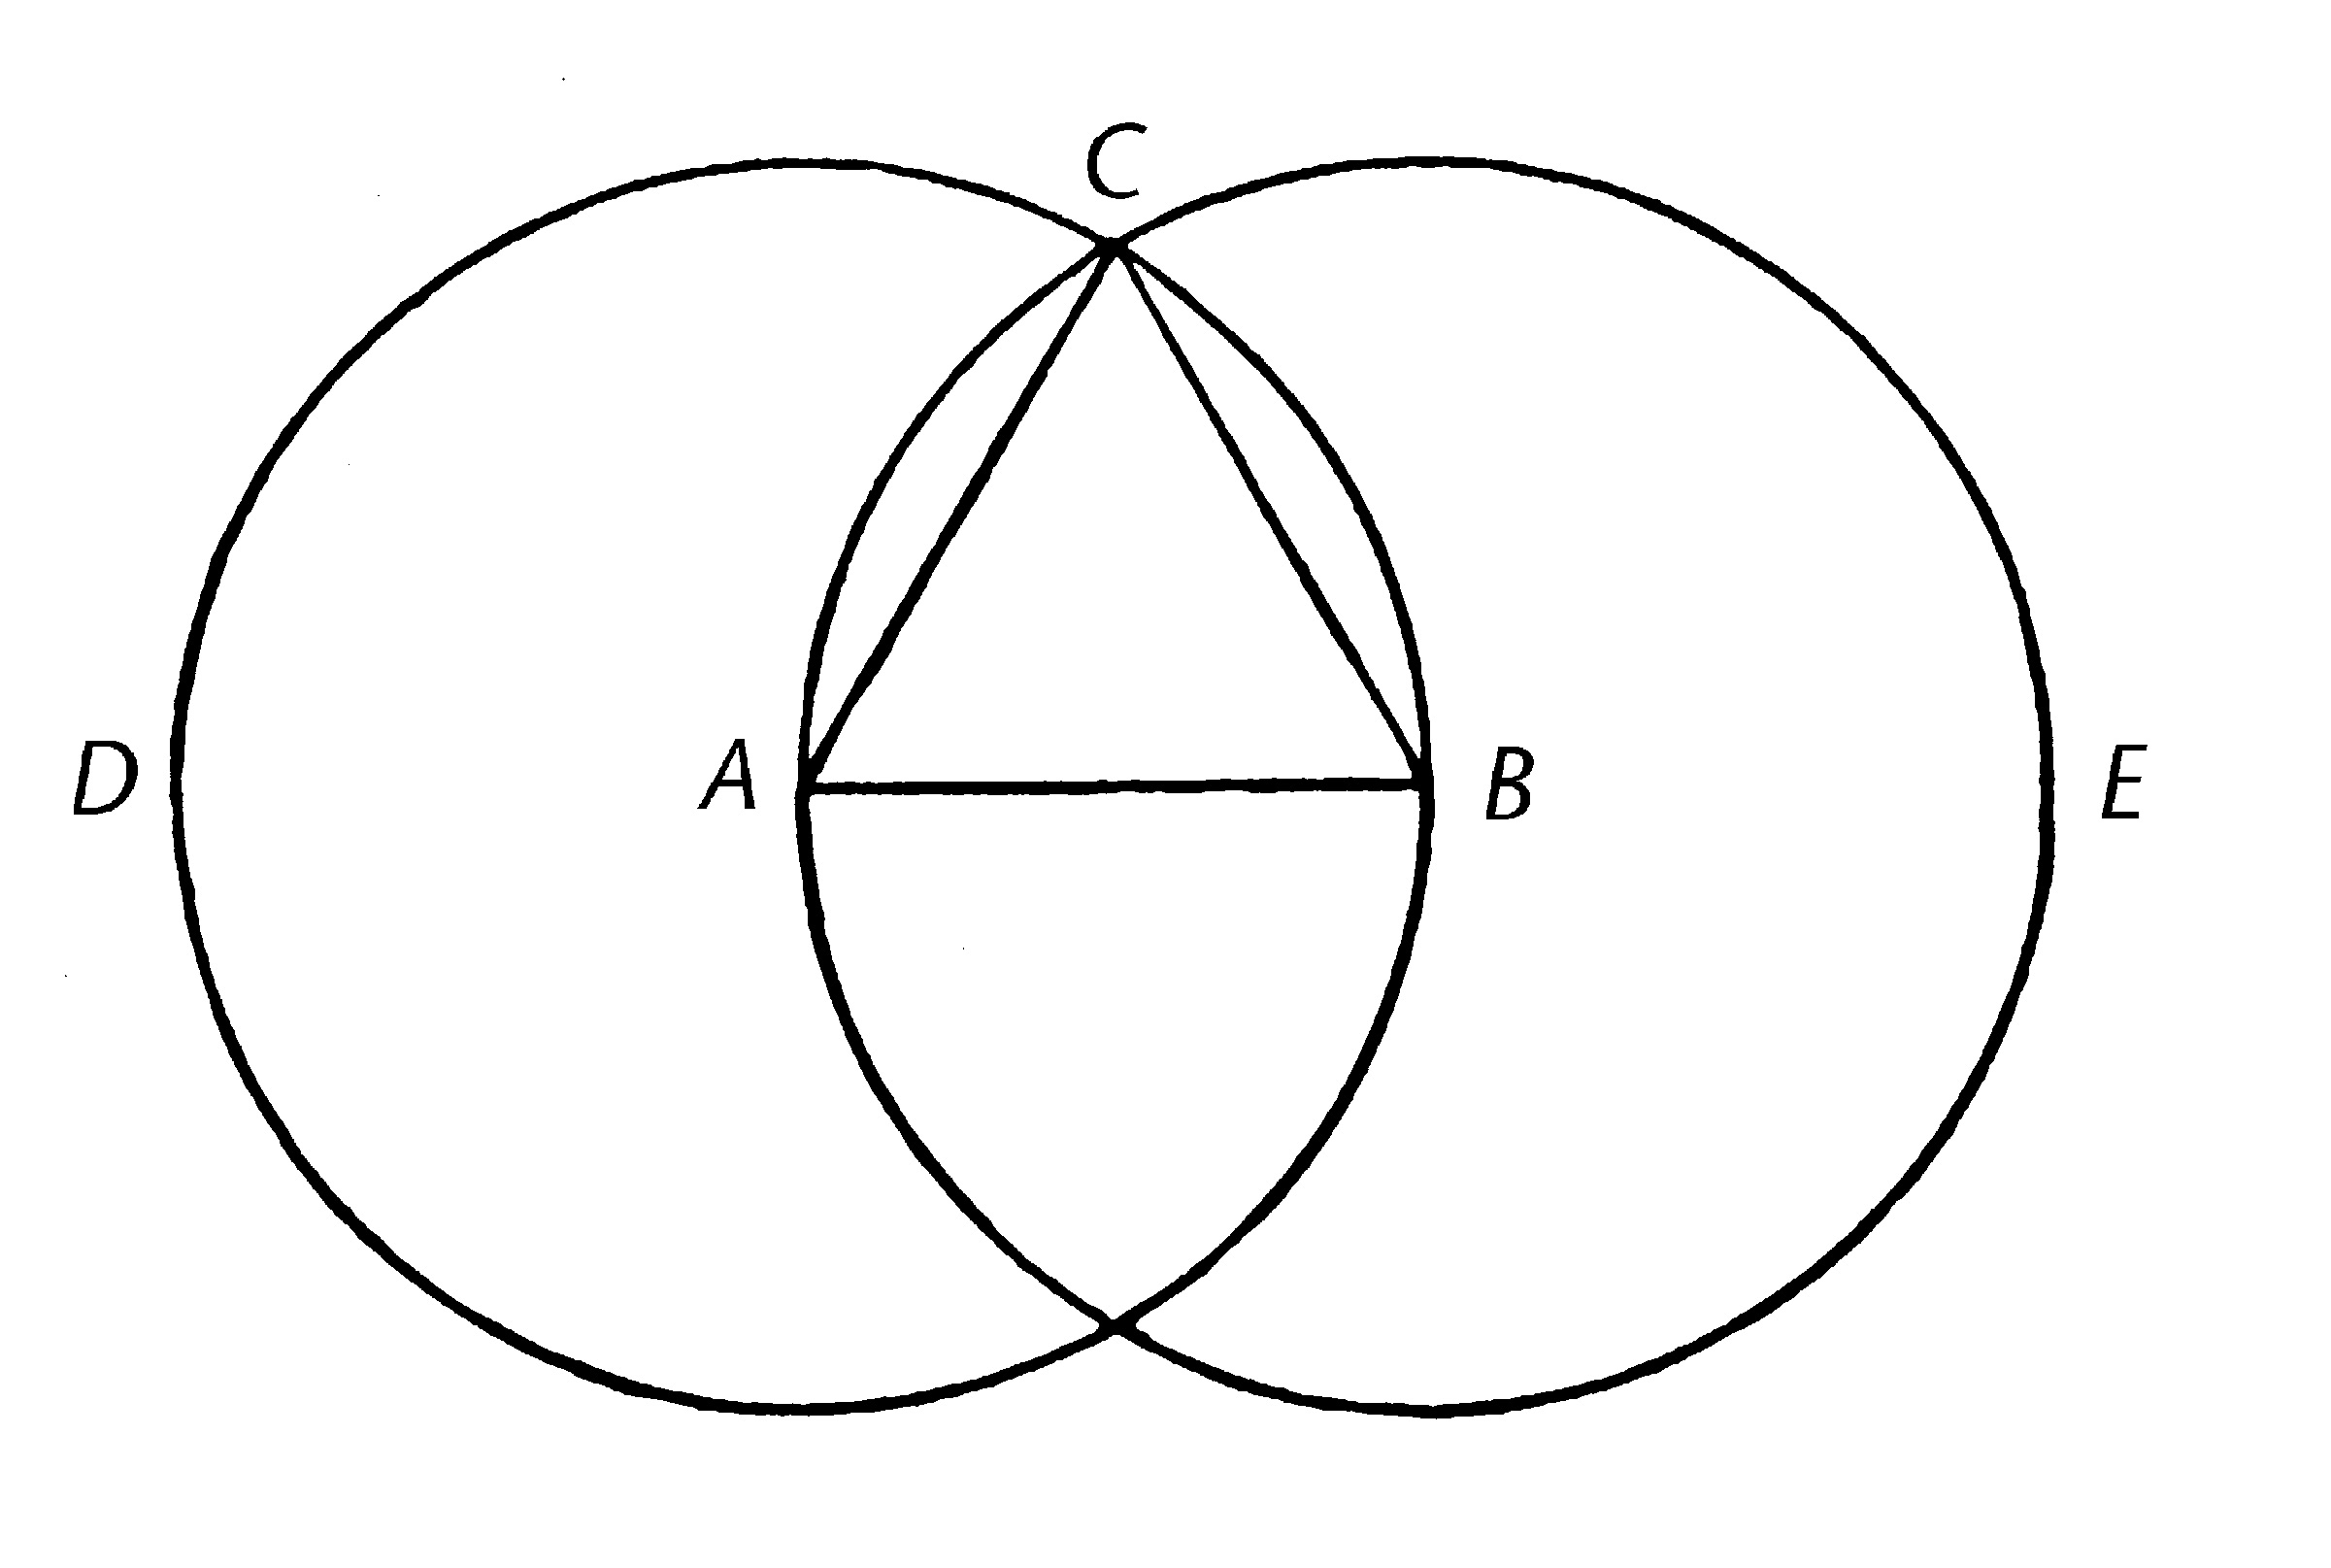
\includegraphics[width=0.4\linewidth]{./image/0}

设AB是给定的有限直线。

那么需要在直线AB上构建一个等边三角形。以A为圆心,AB为距离,画圆BCD。【公设3】

再一次,以B为圆心,BA为距离,画圆ACE;【公设3】并且从点C,两圆相交的地方,到点AB,连接线段CA, CB. 【公设1】

现在,因为点A是圆CDB的圆心,所以AC等于AB。【定义15】

再一次,因为点B是圆CAE的圆心,所以BC等于BA。【定义15】

但是CA已被证明相等于AB,所以线段CA,CB都等于AB。

而且与同一事物相等的事物彼此互等【公理1】;所以CA等于CB。

所以三条线段CA, AB, BC彼此之间互等。

所以三角形ABC是等边三角形,并且它是被构建在指定的线段AB上。

这就是被要求作的。

问题示例:

``并且从点C,两圆相交的地方'': 我们如何知道两圆会相交?

我们如何知道两圆相交在一点?

\hypertarget{ux547dux9898ux4e8c}{%
\section{命题二}\label{ux547dux9898ux4e8c}}

\textbf{由给定一点{[}作为端点{]}作一线段,使与一给定线段相等。}

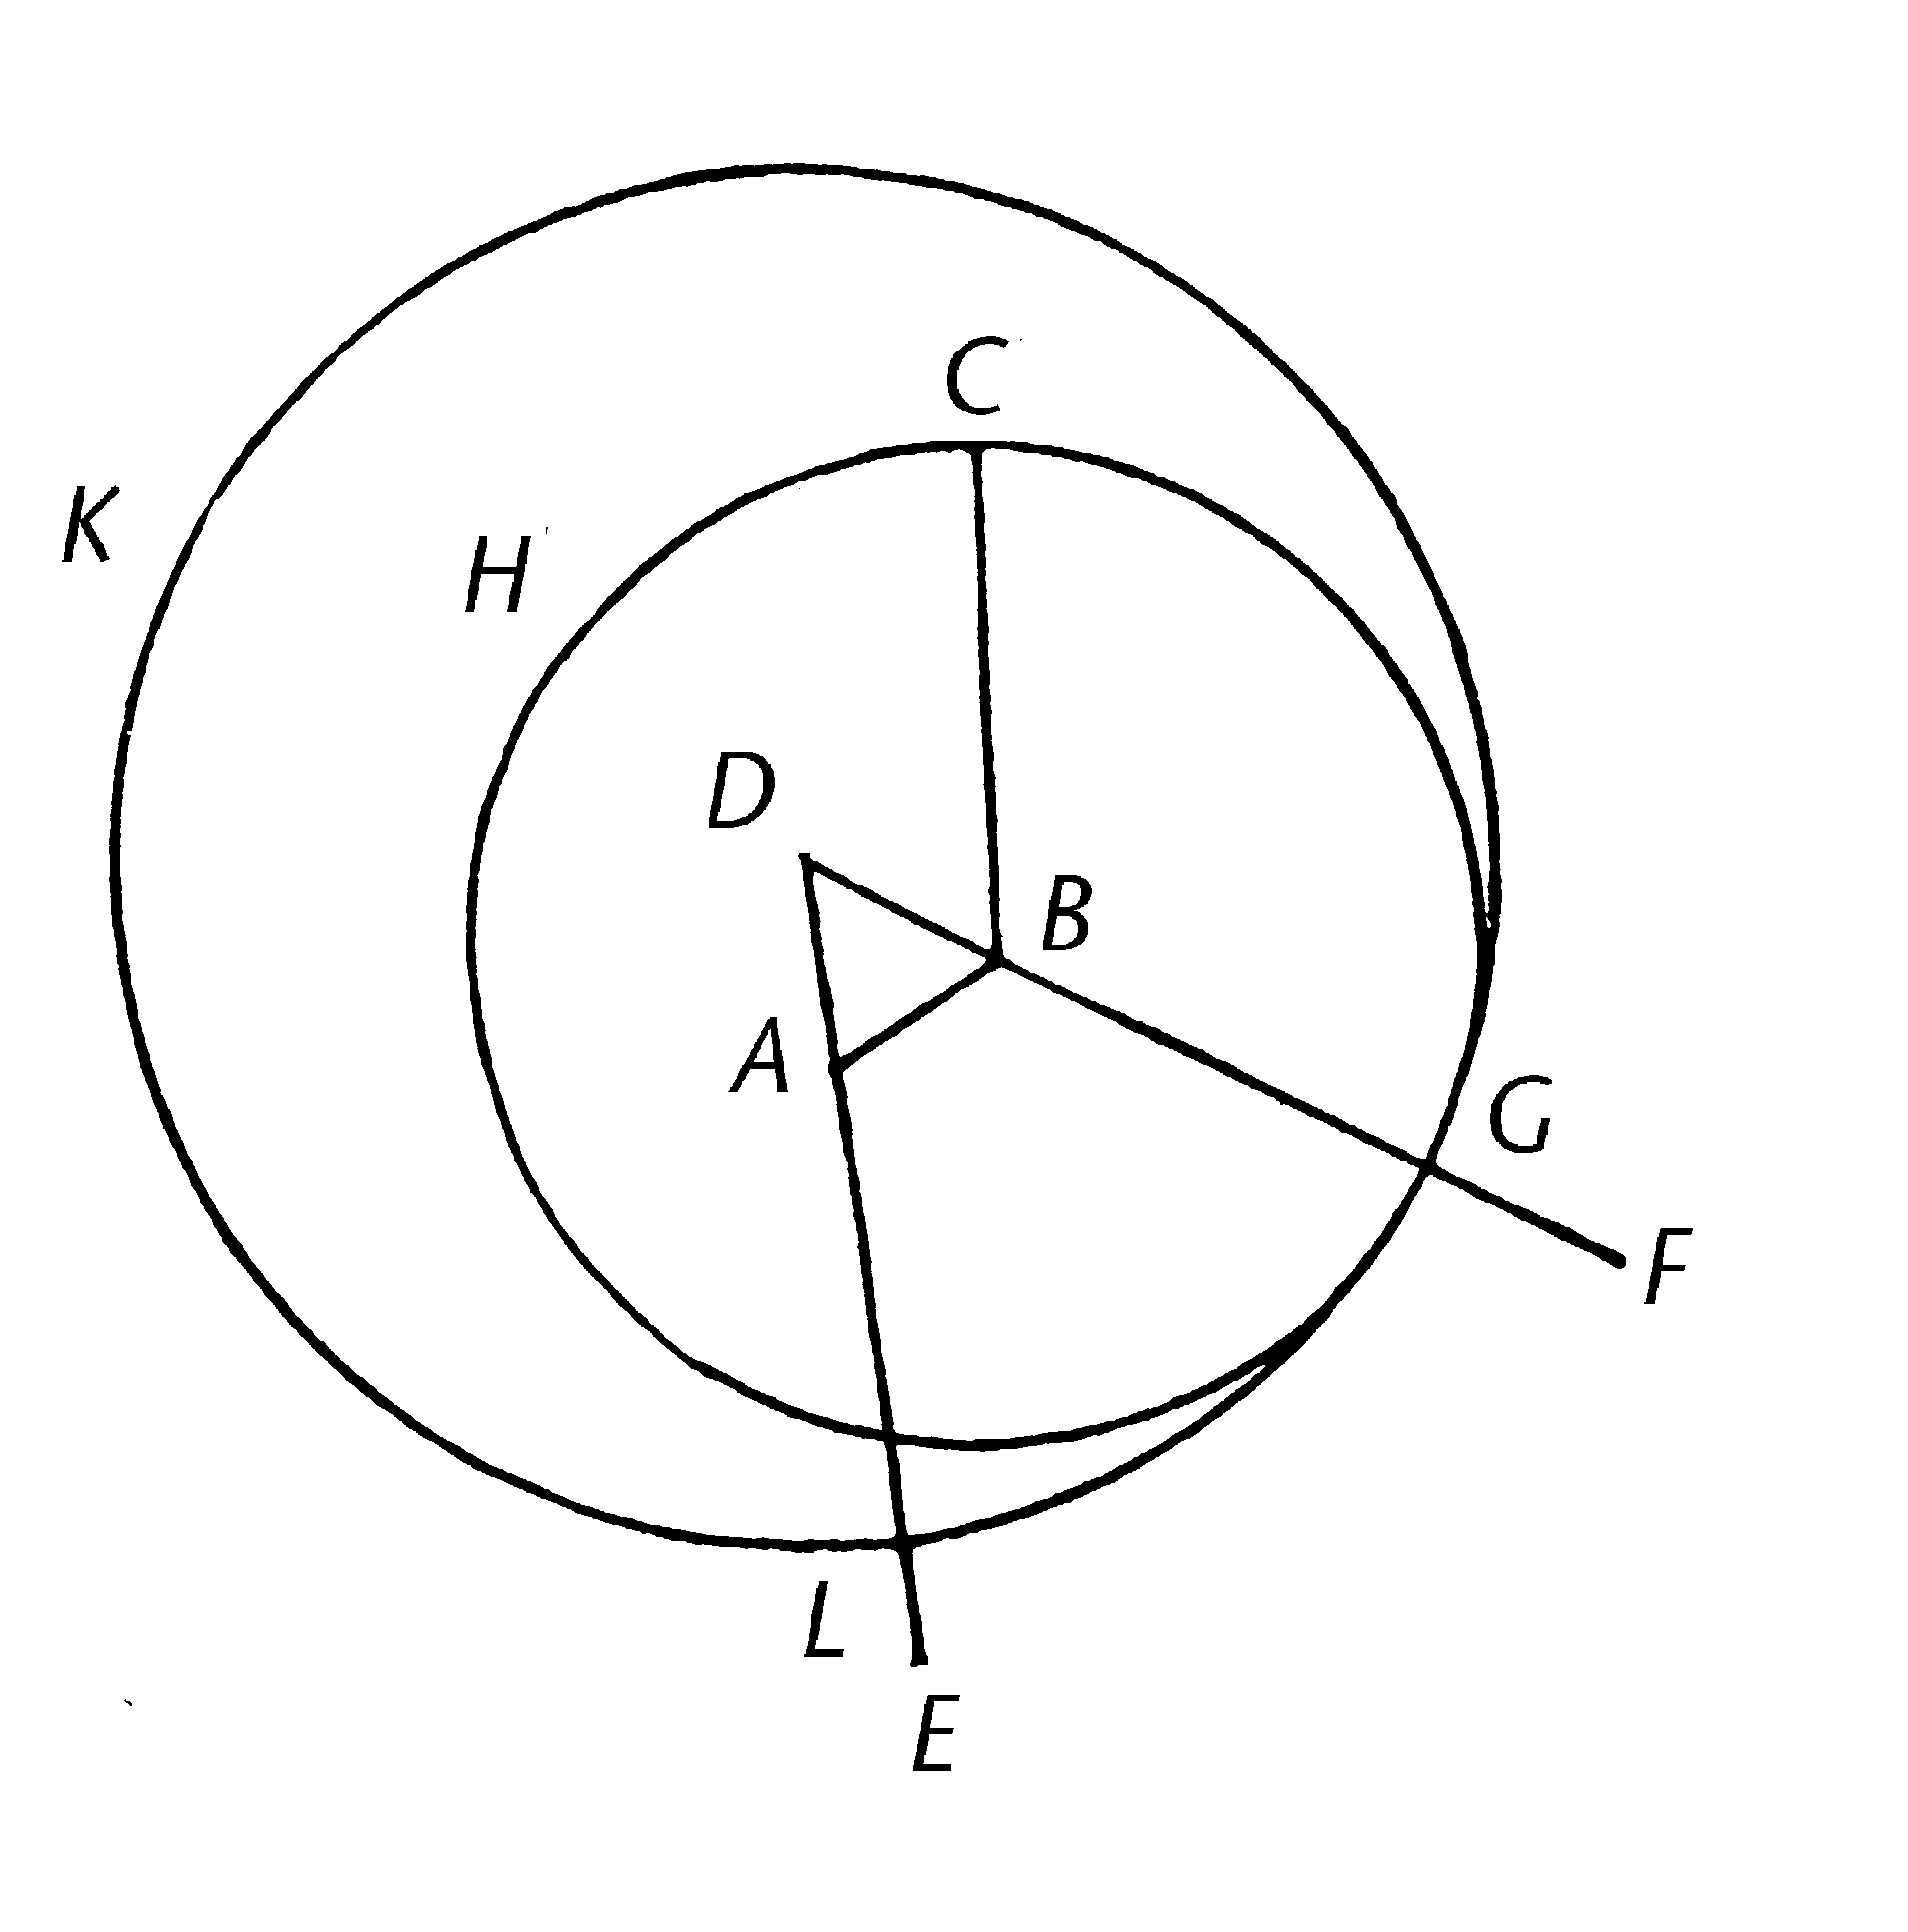
\includegraphics[width=0.3\linewidth]{./image/img447}

使A作为给定一点,BC为给定线段。

那么要求由给定一点A(作为端点)作一线段,使与线段BC相等。

从点A到点B,连接线段AB。【公设1】并且在其上构建等边三角形DAB。【I.1】

延长DA,DB至直线AE,BF. 【公设2】

以B为圆心,BC为距离,画圆CGH;【公设3】

且再一次,以D为圆心,DG为距离,画圆GKL。【公设3】

那么,因为B是圆CGH的圆心,所以BC等于BG。

再一次,因为D是圆GKL的圆心,所以DL等于DG.

且其中DA等于DB;所以余量AL等于BG。【公理3】

但是已证明BC等于BG;所以AL,BC分别等于BG。

而且与同一事物相等的事物们彼此互等【公理1】;所以AL等于BC。

所以由给定点A,作线段AL,等于给定线段BC。

这就是被要求作的。

{[}编者注:这里是Heath提供的,增添以作说明,其实并没有呈现在古希腊语原文中。{]}

\hypertarget{ux547dux9898ux4e09}{%
\section{命题三}\label{ux547dux9898ux4e09}}

\textbf{给定两条不等线段,从长的线段中截取一条线段,使等于短的线段。}

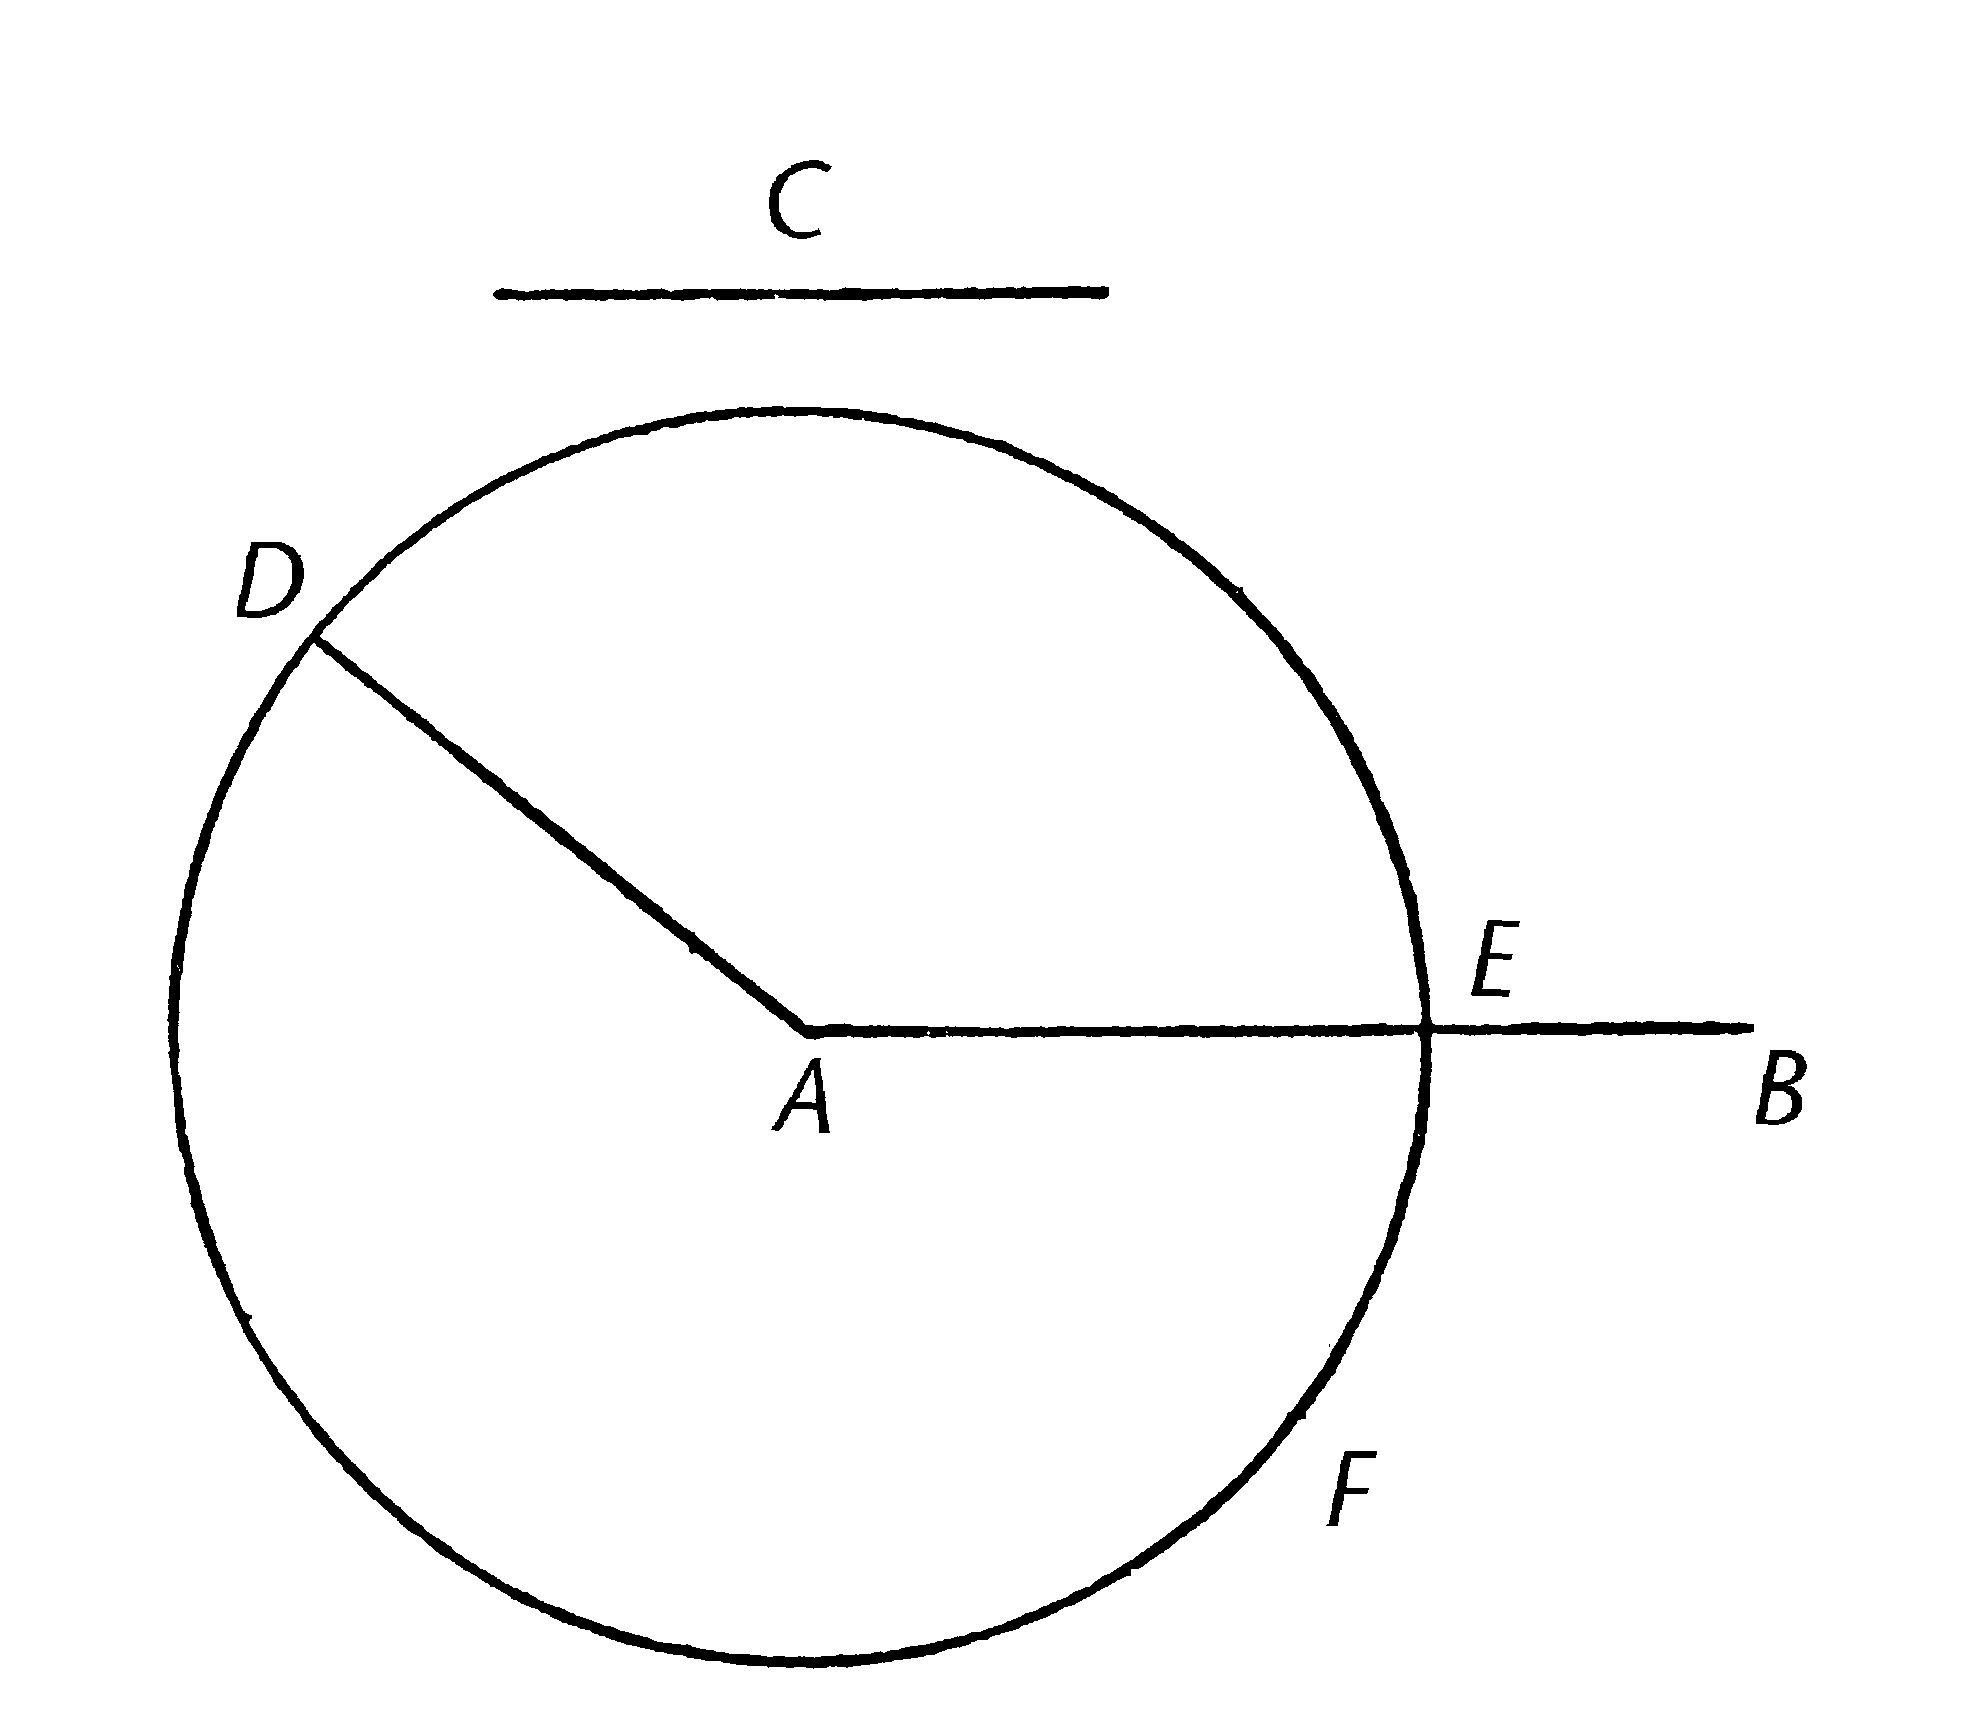
\includegraphics[width=0.3\linewidth]{./image/img449}

设AB,C为两条给定不等线段,AB为长的那条。

那么需要从长线段AB中截取线段与短线段C相等。

从点A取AD等于线段C;【I.2】并且以A为圆心,AD为距离,画圆DEF【公设3】

现在,因为A是DEF的圆心,所以AE等于AD 【定义15】

但是C也等于AD,

所以线段AE,C与AD互等;所以AE也等于C。【公理1】

所以,给定的两条线段AB,C,从长线段AB中,已截取AE与短线段C相等。

这就是被要求作的。

问题示例:

\begin{itemize}
\item
  你有好奇为什么欧几里得的第一步是展示如何构建一个等边三角形么?你有发现命题2关于点A和随机线段BC有些奇怪?现在你在的位置可以感受到愉悦,因为你看到了他是如何小心翼翼地构建他的系统。他用公设和公理证明了命题一,用公设、公理以及命题一,他证明了命题二。现在,用命题二(还有公设3以及公理1),他是不是,通过不相等的线,证明了一个会对处理大小问题有用的事物呢?
\item
  公理3说我们可以以任何圆心和距离画圆。那么,为什么我们不能仅仅用距离C作为给定距离和线段AB的其中一个端点呢?为什么我们需要命题2,是因为在公理3中,我们有给定的举例,而在命题3中,我们只有一个线段么?
\end{itemize}

【宣棋注:greater/less 在中文中,视情况翻译成多少,大小,长短。】

\hypertarget{ux547dux9898ux56db}{%
\section{命题四}\label{ux547dux9898ux56db}}

\textbf{如果两个三角形中两条边互等【】,并且这些互等的边所夹的角也相等,那么他们的底边也互等,三角形全等,剩余的等边所对的角也互等。}

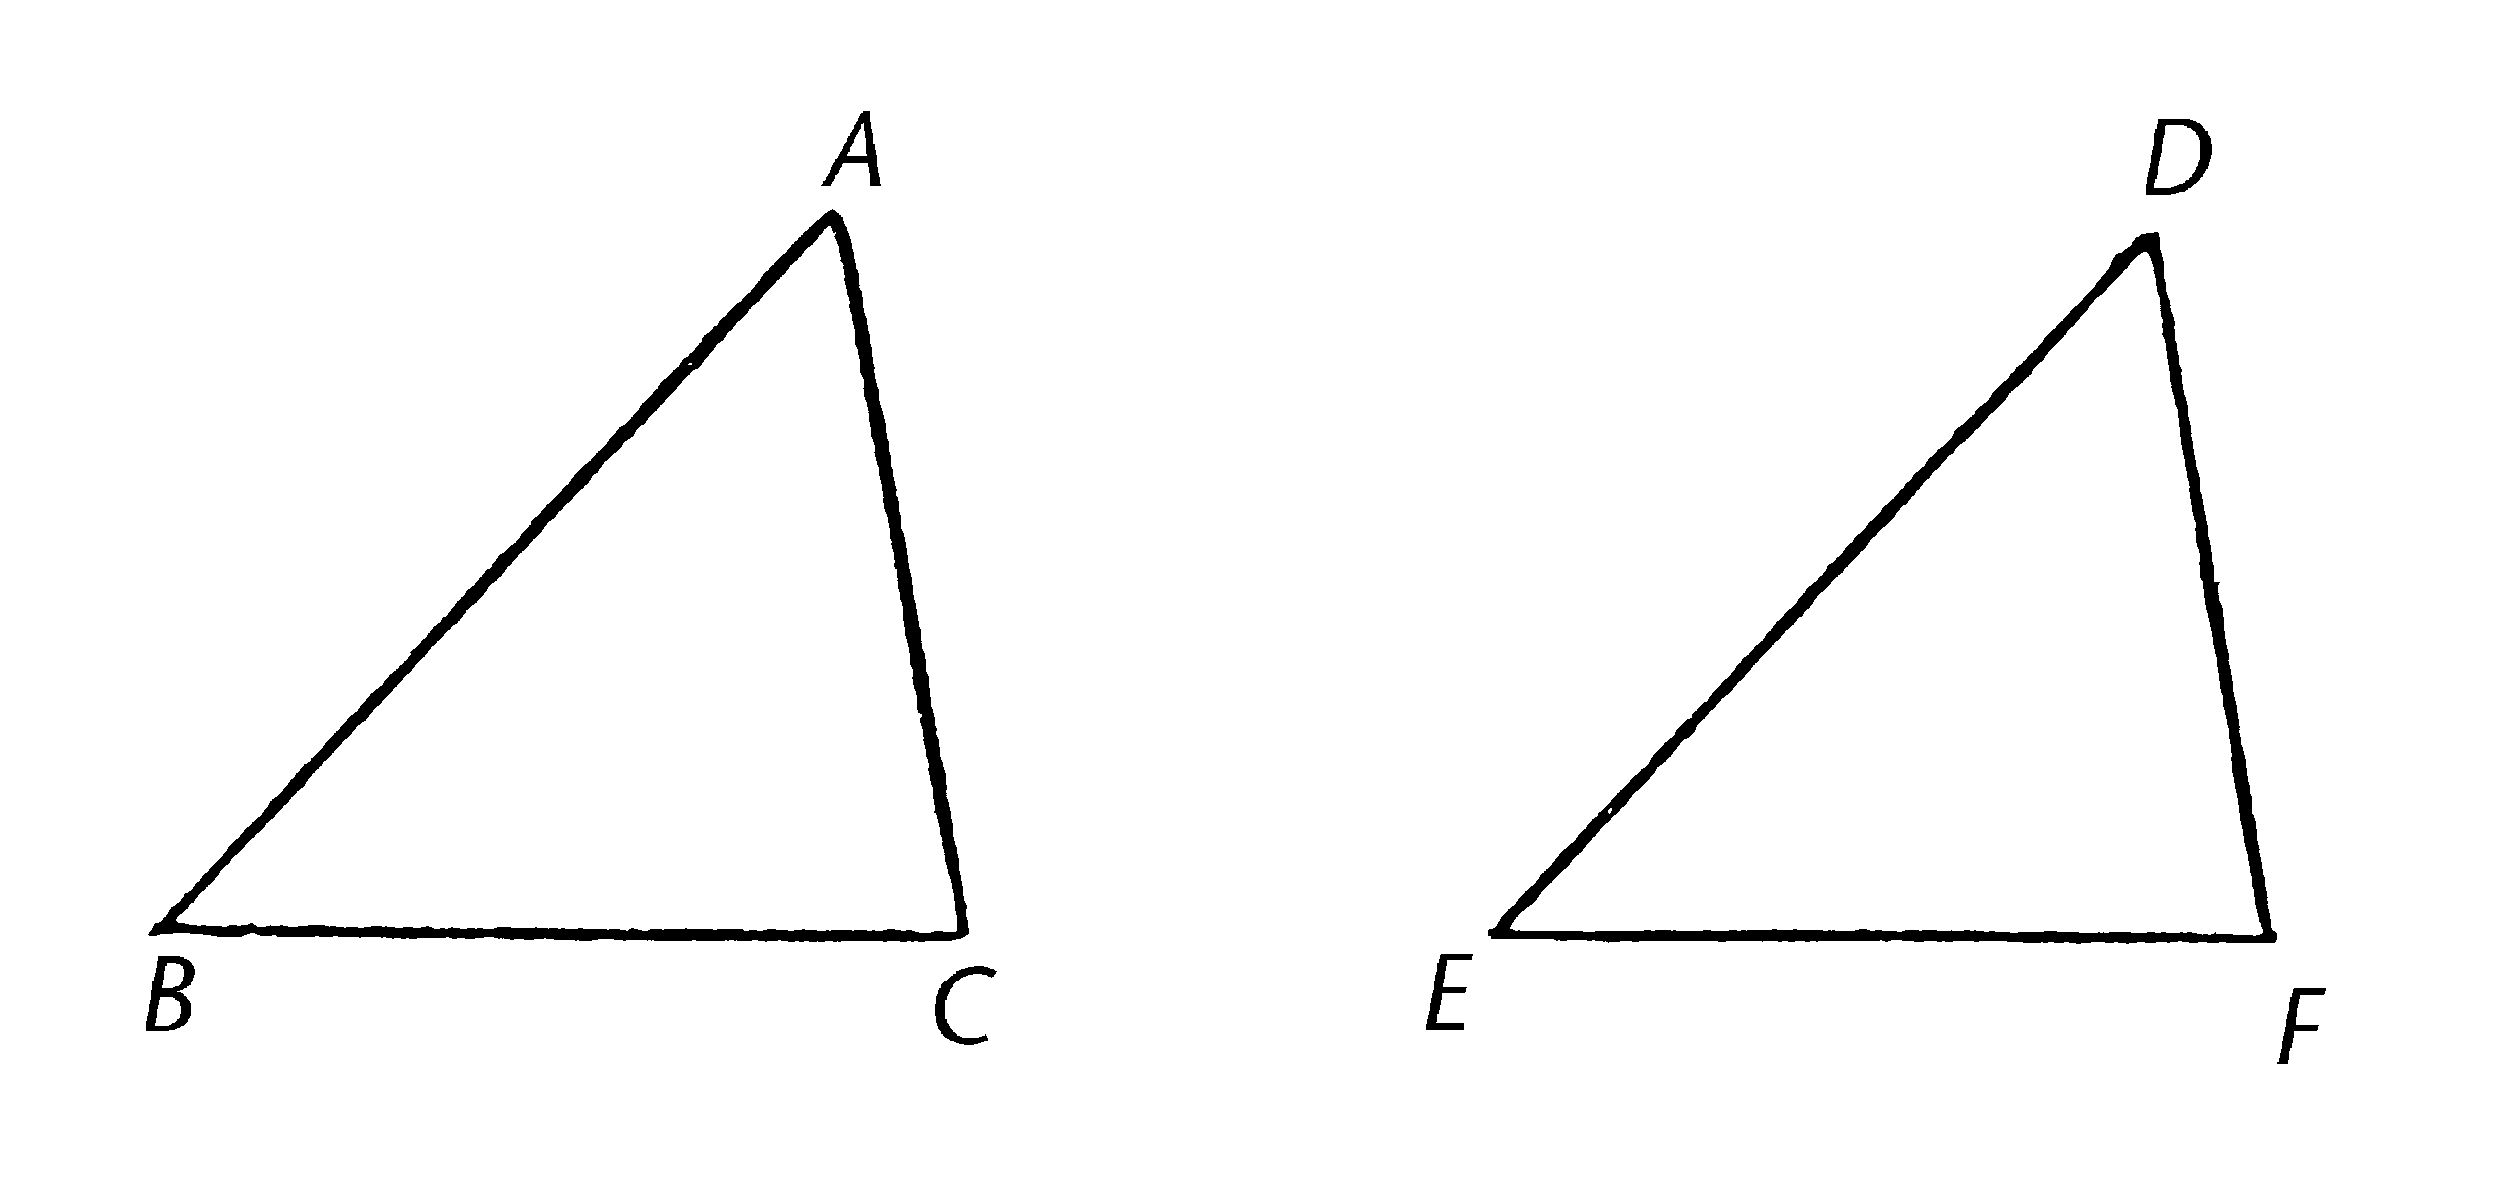
\includegraphics[width=0.5\linewidth]{./image/img451}

设三角形ABC和DEF中,AB,AC分别与DE,DF相等,即AB与DE,AC与DF,并且角BAC等于角EDF。

我说底边BC也等于底边EF,三角形ABC全等于三角形DEF,并且剩余的等边对的角也各自互等,也就是角ABC等于角DEF,角ACB等于角DFE。

因为,如果将三角形ABC放置在三角形DEF上,如果点A放在点D上,线段AB放在DE上,那么点B会与E重合,因为AB等于DE。

再一次,因为如果AB重合DE,那么线段AC重合DF,因为角BAC等于角EDF;

所以点C也重合于点F,因为AC等于DF。

但是B也重合于E,所以底边BC也重合底边EF,并且与之相等。 【公理4】

所以整个三角形ABC重合于整个三角形DEF,并且与之相等。【公理4】

而且剩余的角也各自重合和相等。角ABC和角DEF,角ACB和角DFE。 【公理4】

综上所述\ldots*

Q.E.D.

*编者注:``综上所述\ldots{}''以及关于Q.E.D. 和Q.E.F.的缩写已在前文中解释。

【宣棋注1:这里指的是,其中一个三角形的两边与另一个三角形的两边分别相等】

【宣棋注2:在原文中,并没有三角形``全''等的``全''这个词,是为了和中文中的术语保持一致,决定这么翻译。这个命题就是几何中由SAS证全等的由来。】

问题示例:

\begin{itemize}
\tightlist
\item
  前三个命题是关于做的事情。现在我们转移到了许多论证事情的命题中的第一个。你如何看待这里的不同:探究方法、策略、语言?
\item
  这是他第一次在陈述声明之后说``我说\ldots''。 为什么他在论证之间说这个?是因为在之前的命题中,他断言了独立于他的真理么?而且这样做,你就会拥有真理。而在这个还有之后的命题里,他对声明的陈述以及提出论据负有责任?通过这样的做法,在你看到论证的最后,被说服之前,是都不需要相信他的么?
\item
  这里是断言面积相等的首次出现。(``三角形全等'',并且我们知道图形是被边界围成的)通过这本书,欧几里得将要建立更多关于面积相等复杂的论断。
  这里的基石是重合,根据公理4彼此重合的事物相等。在建立体系的此处,我们已经用到了简单的前三条算术公理,现在则是公理4,有些不同的重合准则。之后,我们也会调用已定义(定义十)和假设(假设四)的直角相等性。
\item
  这也是第一个关于一致性的证明。你能想到其它无需重合,证明面积、剩余的角、还有底边相等的方法么?
\item
  我们怎样才能知道这些三角形、点、线段、角可以彼此重合呢?我们不能把三角形拾起然后放到另一个上面。你怎么看待他的论据,关于他在脑海中将点放置重合,然后放线段和角重合?逐步做这个可以避免想象中的怪异------我们可以在不改变三角形的情况下拾起并且移动它?
\item
  如果这个结论是承接着公理4,为什么我们需要这个命题?仅仅是因为我们要展示它们彼此重合?如果是这样的话,我们需要更仔细的察看措辞:每一步的已知和所求。
\item
  这些步骤本身需要授权么?特别是当他说B与E重合因为它们长度相等时?这些步骤确实看起来可以被立刻推论,但事实上线段不重合是很难想象的。如果他们不重合的话,两条线段就会围成一个空间。你能通过组合先前的元素,比如定义4,公设1和2,还有公理4,从逻辑推导出线段的重合么?或者说这里还是缺少了什么?
\item
  也有人建议说欧几里得应该将卷一命题命题四作为一个假设。你认为欧几里得为什么始终将此作为一个命题?
\item
  如果允许拿起某物并且移动它,在前三个命题中,为什么我们不能拿起那些线段并且移动他们呢?他们的情况有何不同?或者说只是欧几里得对他的方法感到不适,并且只会在别无选择时这样做?(后面仅有两个地方会呈现:卷一命题4和命题8)
\item
  那么我们能否确认三角形在被移动的过程中不会发生改变?而且当我们已经确定两个叠加的三角形全等,如何将其拓展到那些不叠加的三角形?
\end{itemize}

\hypertarget{ux547dux9898ux4e94}{%
\section{命题五}\label{ux547dux9898ux4e94}}

\textbf{在等腰三角形中,两底角互等,并且如果两腰继续延伸,底边下的两角也互等。}

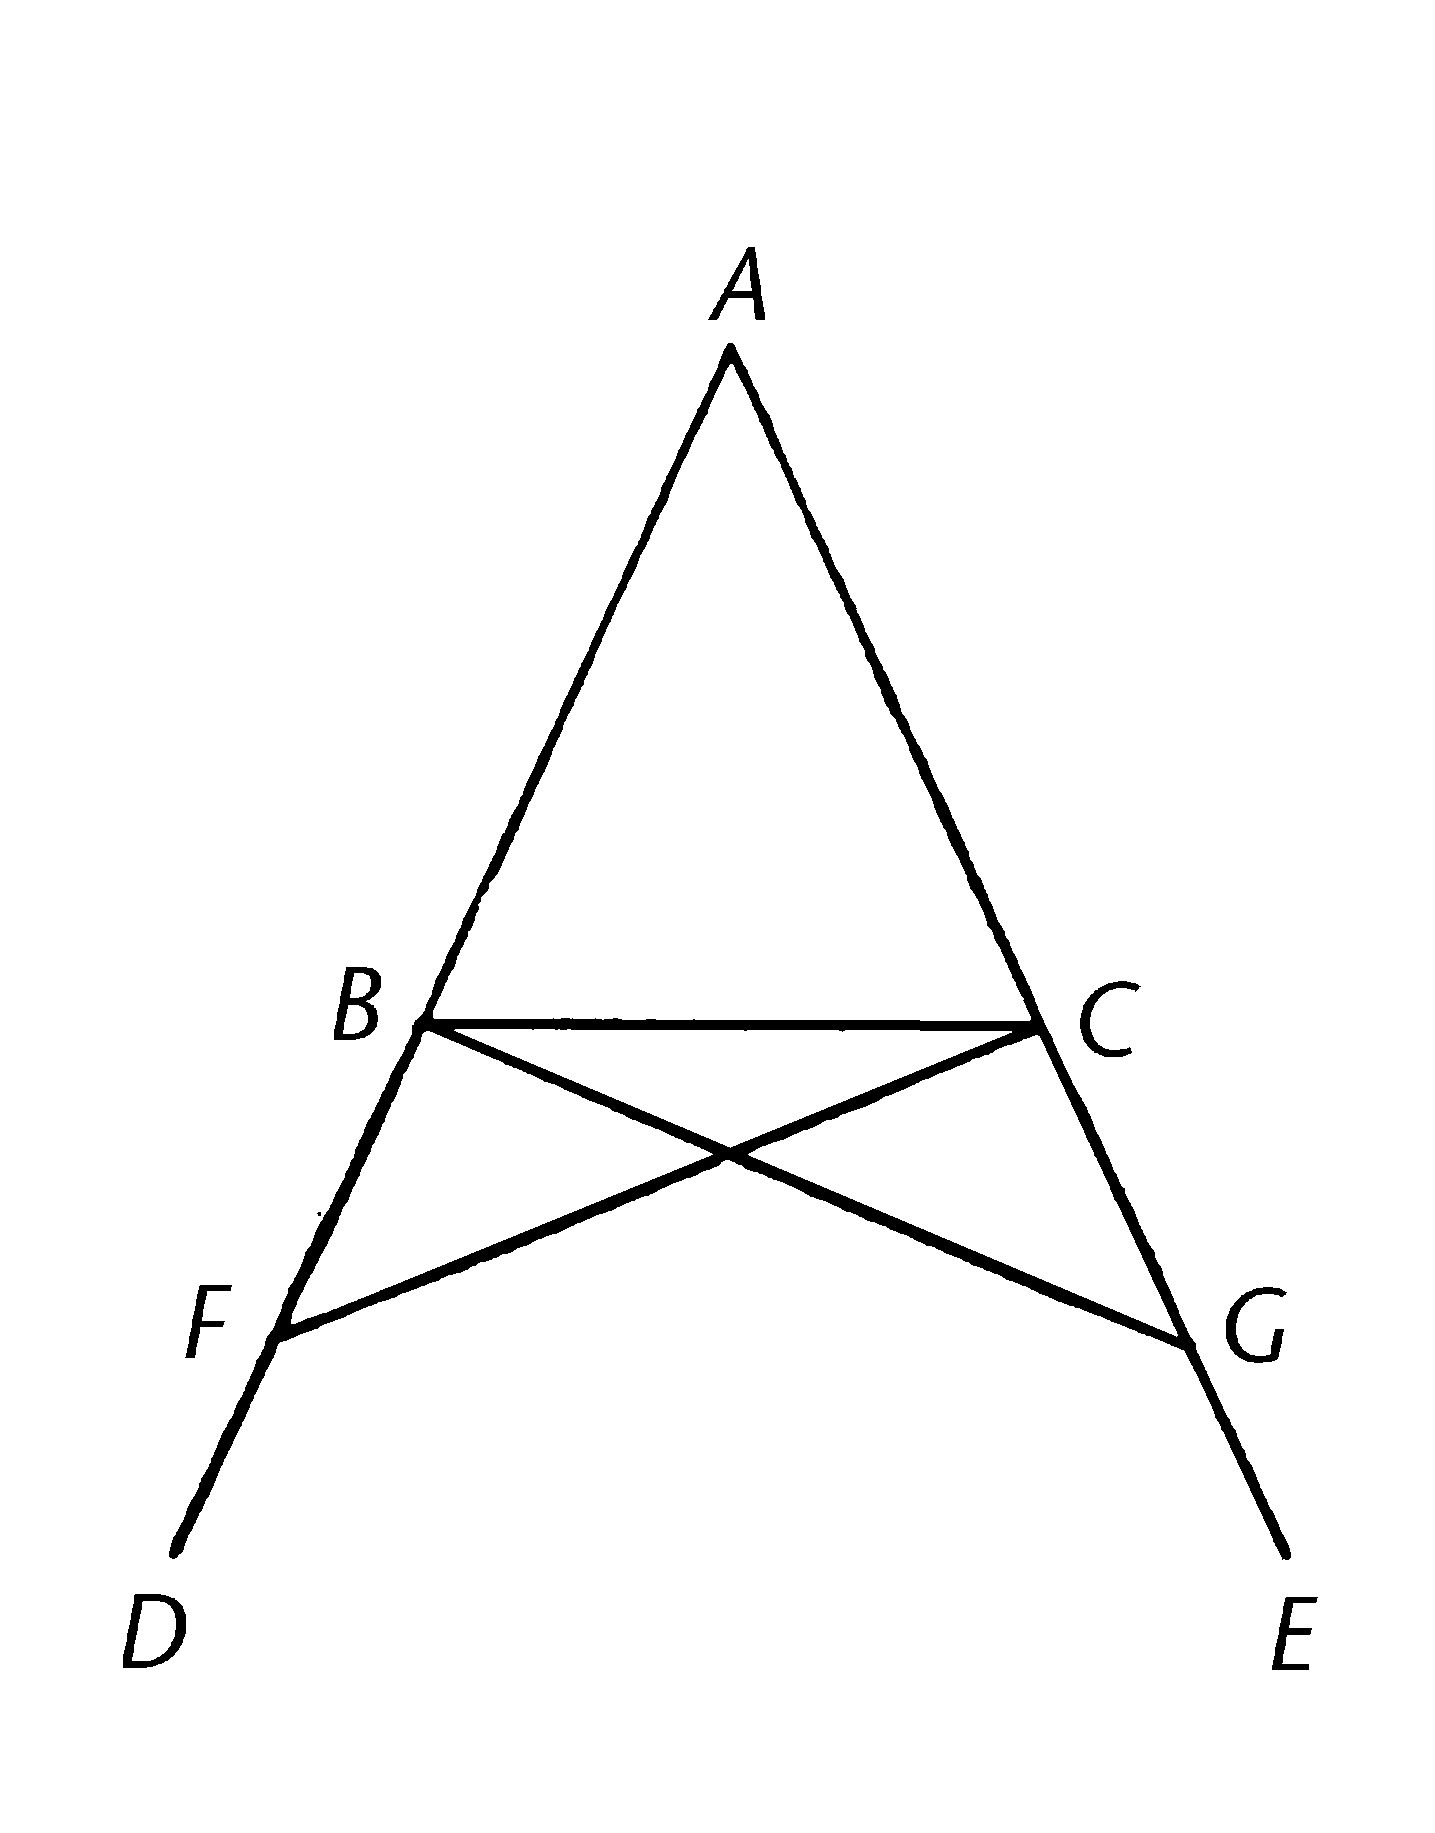
\includegraphics[width=0.25\linewidth]{./image/img455}

设等腰三角形ABC中边AB等于AC;设直线BD,CE是AB,AC同直线的延伸。【公设2】

我说角ABC等于角ACB,并且角CBD等于角BCE。

在BD上任取一点F,从长线段AE上截取AG,使之等于短线段AF;【I.3】并且连接线段FC,GB。

那么,因为AF等于AG,AB等于AC,两条边FA,AC各自与两条边GA,AB相等;并且他们包含一个共同的角FAG。

所以底边FC等于底边GB,三角形AFC全等于三角形AGB,并且和剩余的各等边相对的角也各自相等,也就是说角ACF等于角ABG,角AFC等于角AGB。【I.4】

且因为作为整体,AF等于AG,其中AB等于AC,那么剩余的部分BF等于CG。

但是FC也被证明与GB相等,所以两条边BF,BC与另两条边CG,GB互等;角BFC等于角CGB,同时BC是公共的底边;所以三角形BFC也全等于三角形CGB,并且剩余等边所对的角也各自相等,所以角FBC等于角GCB,角BCF等于角CBG。

相应的,因为作为整体的角ABG已被证明等于角ACF,其中角CBG等于角BCF,剩余的部分角ABC等于剩余的部分角ACB;并且他们在三角形ABC的底边上。

但是角FBC已被证明等于角GCB,且他们在底边下。

综上所述\ldots{}

Q.E.D.

问题示例:

\begin{itemize}
\tightlist
\item
  这是否让人惊讶:他先证明了第二部分?你是否曾期待用更明显的事实------底边内两角相等,作为基石证明底边两外角相等,而不是相反的方式?这个简单的例子也许已经暗示了独辟蹊径的创造力可能会被用于证明更复杂的命题。
  【宣棋注:这个问题是问我们是否对先证明底边下两角相等再证明两腰所对相交互等感到惊讶。】
\end{itemize}

\hypertarget{ux547dux9898ux516d}{%
\section{命题六}\label{ux547dux9898ux516d}}

\textbf{如果三角形中两角互等,那么两角各自对应的边也互等。}

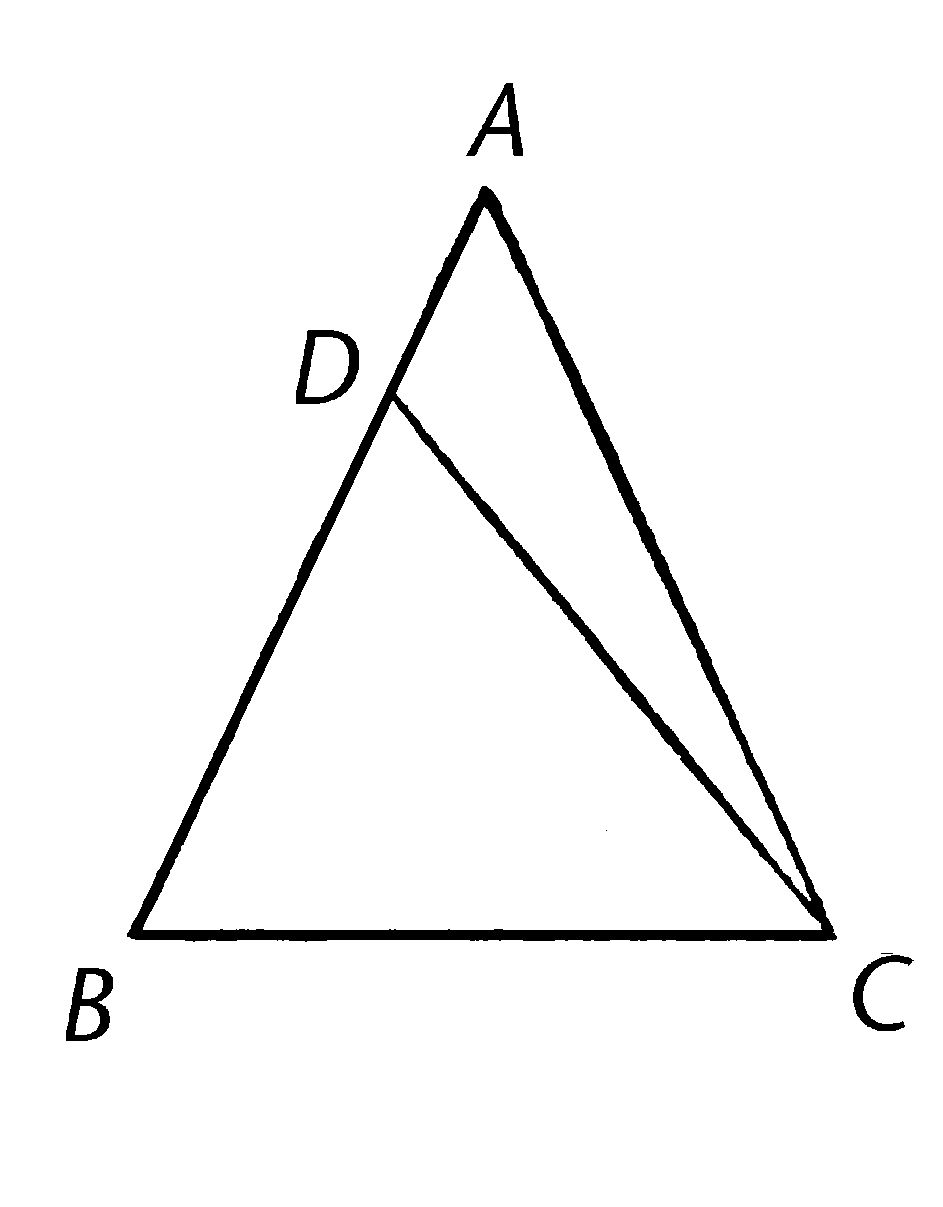
\includegraphics[width=0.25\linewidth]{./image/img458}

设三角形ABC中角ABC等于角ACB; 我说边AB等于边AC。

因为如果AB不等于AC,他们其中之一会更长。

设AB更长;在长线段AB中截取DB,使之与短线段AC相等;连接DC。

那么,因为DB等于AC,并且BC是公有的,两边DB,BC各自与两边AC,CB互等,并且角DBC等于角ACB;所以底边DC等于底边AB,且三角形DBC与三角形ACB全等,小的等于大的:这是不合逻辑的。

所以AB不能不等于AC;所以两者相等。

综上所述\ldots{}

Q.E.D.

问题示例:

\begin{itemize}
\tightlist
\item
  我们如何知道三角形BDC比三角形BAC小?因为那儿并没有详细的步骤证明它,我们可以依据可以看到的绘画么?
\item
  这个命题介绍了一种新的论证技巧,``reductio ad absurdum'' (reduction to absurdity,归谬法)。如果我们不能找到一个方式直接证明某事,我们可以做相反的假设,然后看是否会引起一个矛盾。
\item
  在这个题中,你能直接证明这个声明么?
\item
  对你来说,归谬的方法是否和直接证明一样有说服力?
\item
  在假设相反情况的时候,会不会有可能的失误或者谬论?会是什么呢?在哪些方面我们应该特别留意?
\item
  如果这里有不止你想证明的那一种情况,你如何才能知道你已经排除了其它可能性?在这个题中,其它的可能性是什么?
\item
  这个证明依赖于公理5``整体大于部分''吗?
\item
  此命题与命题I.5的第一部分相反。你认为为什么他没有收录关于第二部分相反的证明?因为他不需要么?(之后他不会用到那个性质?)还是因为如果需要的话,读者们可以轻松地自行证明它?
\end{itemize}

\hypertarget{ux547dux9898ux4e03}{%
\section{命题七}\label{ux547dux9898ux4e03}}

\textbf{在同一条直线(由它的两端点),构建会在同一点相交的给定两线段,那在同一条直线上(由两端点),在同一侧,不能构建出交于另一点的另两条线段,使之与之前的两线段相等,即分别到每个端点的线段。}

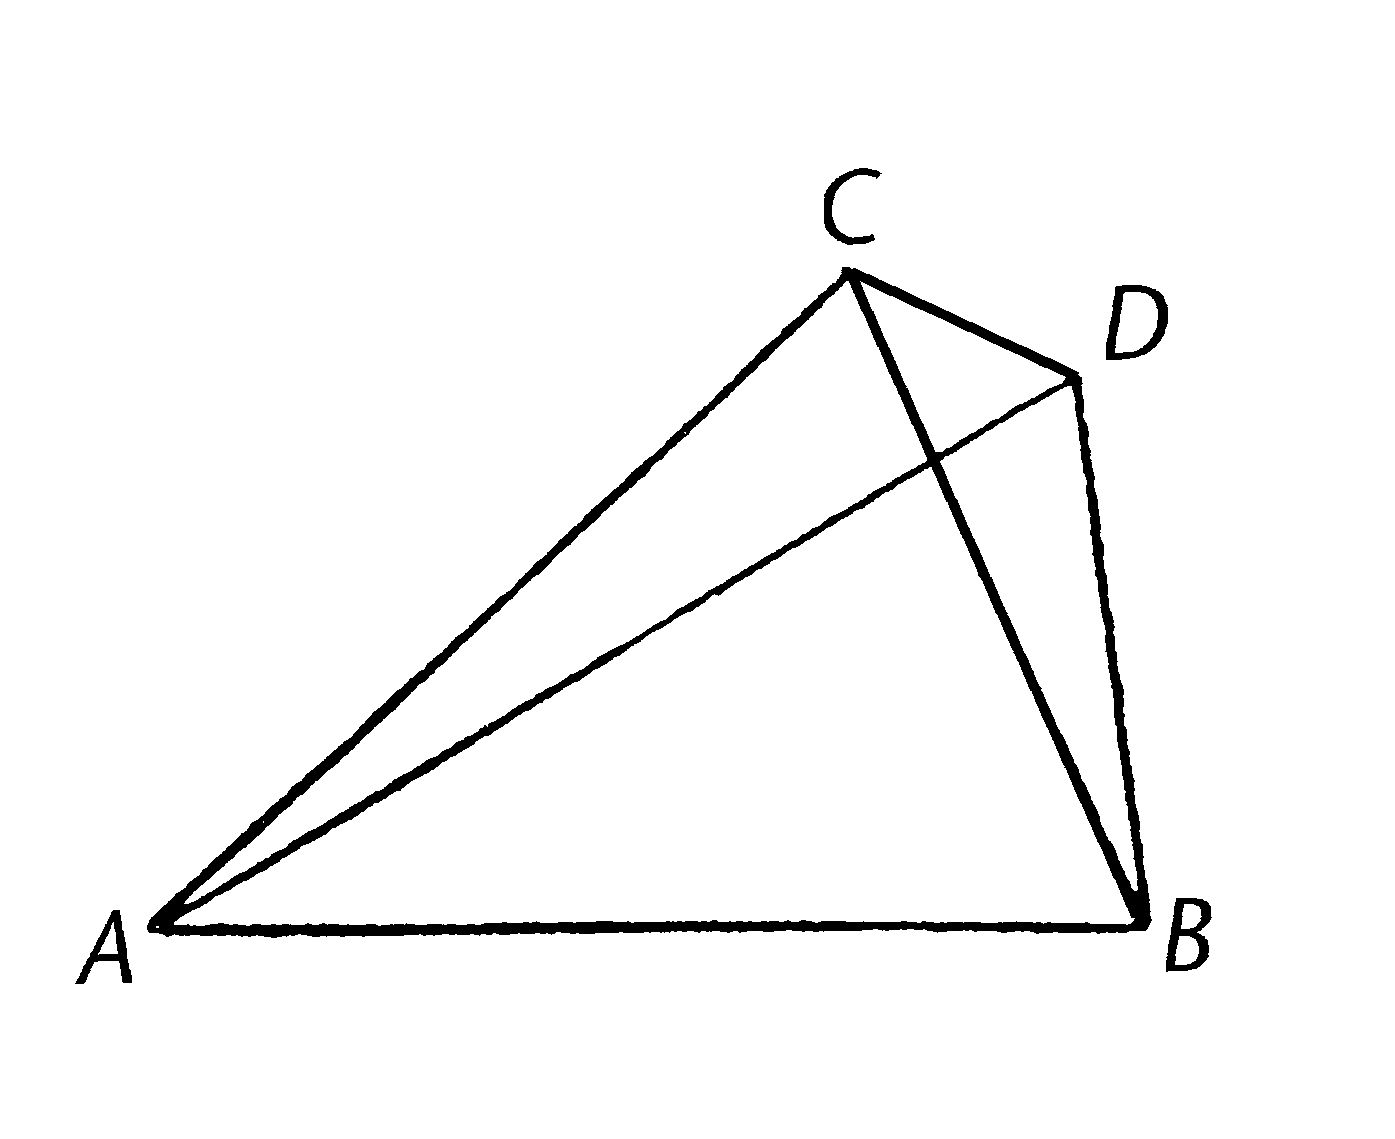
\includegraphics[width=0.3\linewidth]{./image/img461}

因为,如果可能的话,给定在直线AB上构建的两线段AC,CB交于点C,设其它两线段AD,DB构建在相同的直线AB的同一侧上,交于另一点D,并且与之前的两线段相等,也就是彼此到相同的端点,所以CA等于DA,有共同的端点A,而且CB等于DB,有共同的端点B,连接CD。

那么,因为AC等于AD,角ACD也等于角ADC;【I.5】那么角ADC大于角DCB;那么角CDB大于角DCB。

重复地,因为CB等于DB,角CDB也等于角DCB 。

但是已经证明了它更大:这是不可能的。

综上所述\ldots{}

Q.E.D.

问题示例:

\begin{itemize}
\tightlist
\item
  另一个reductio(归谬),我们被``如果可能的话\ldots''所警醒!我们一共有多少种其它选择?可能的和不可能的?各种``不可能的''配置重要么?
\item
  这里是否还有其它情况会改变证明中的步骤?绘画中显示AC是边AC和CB中较长的,所以D落于CB之外。如果AC是较短的边呢?那么绘画会是什么样子?如果他们相等呢?
\item
  从公设的问题示例开始,我们思考通过绘图学习和通过逻辑学习的关系。公设是关于能画的,我们已有的和将有的命题,关于图像的构建,暗示着绘画至少在某种程度上对这个项目时很关键的。
\item
  但是,等一下!绘画会不会产生误导?如果图像只能显示一种情况,但可能有多种呢?比如说,假定图像显示线相交于一边,且命题对这种情况是有效的,但是完成的构建是在另一边或者根本没有相交。
\item
  如果这里还有其它情况,为什么欧几里得没有将他们囊括以作为证明的一部分呢?是否欧几里得只给予一种情况,且将剩余(有类似逻辑或者更简单的情况)留给读者,因为这是不需要讲出的?你能够草绘出其它情况的证明并且确认他们也会出现``不可能的''结果么?
\end{itemize}

\hypertarget{ux547dux9898ux516b}{%
\section{命题八}\label{ux547dux9898ux516b}}

\textbf{如果两个三角形分别有两边各自对应相等,并且底边也互等,那么被等边夹的角也互等。}

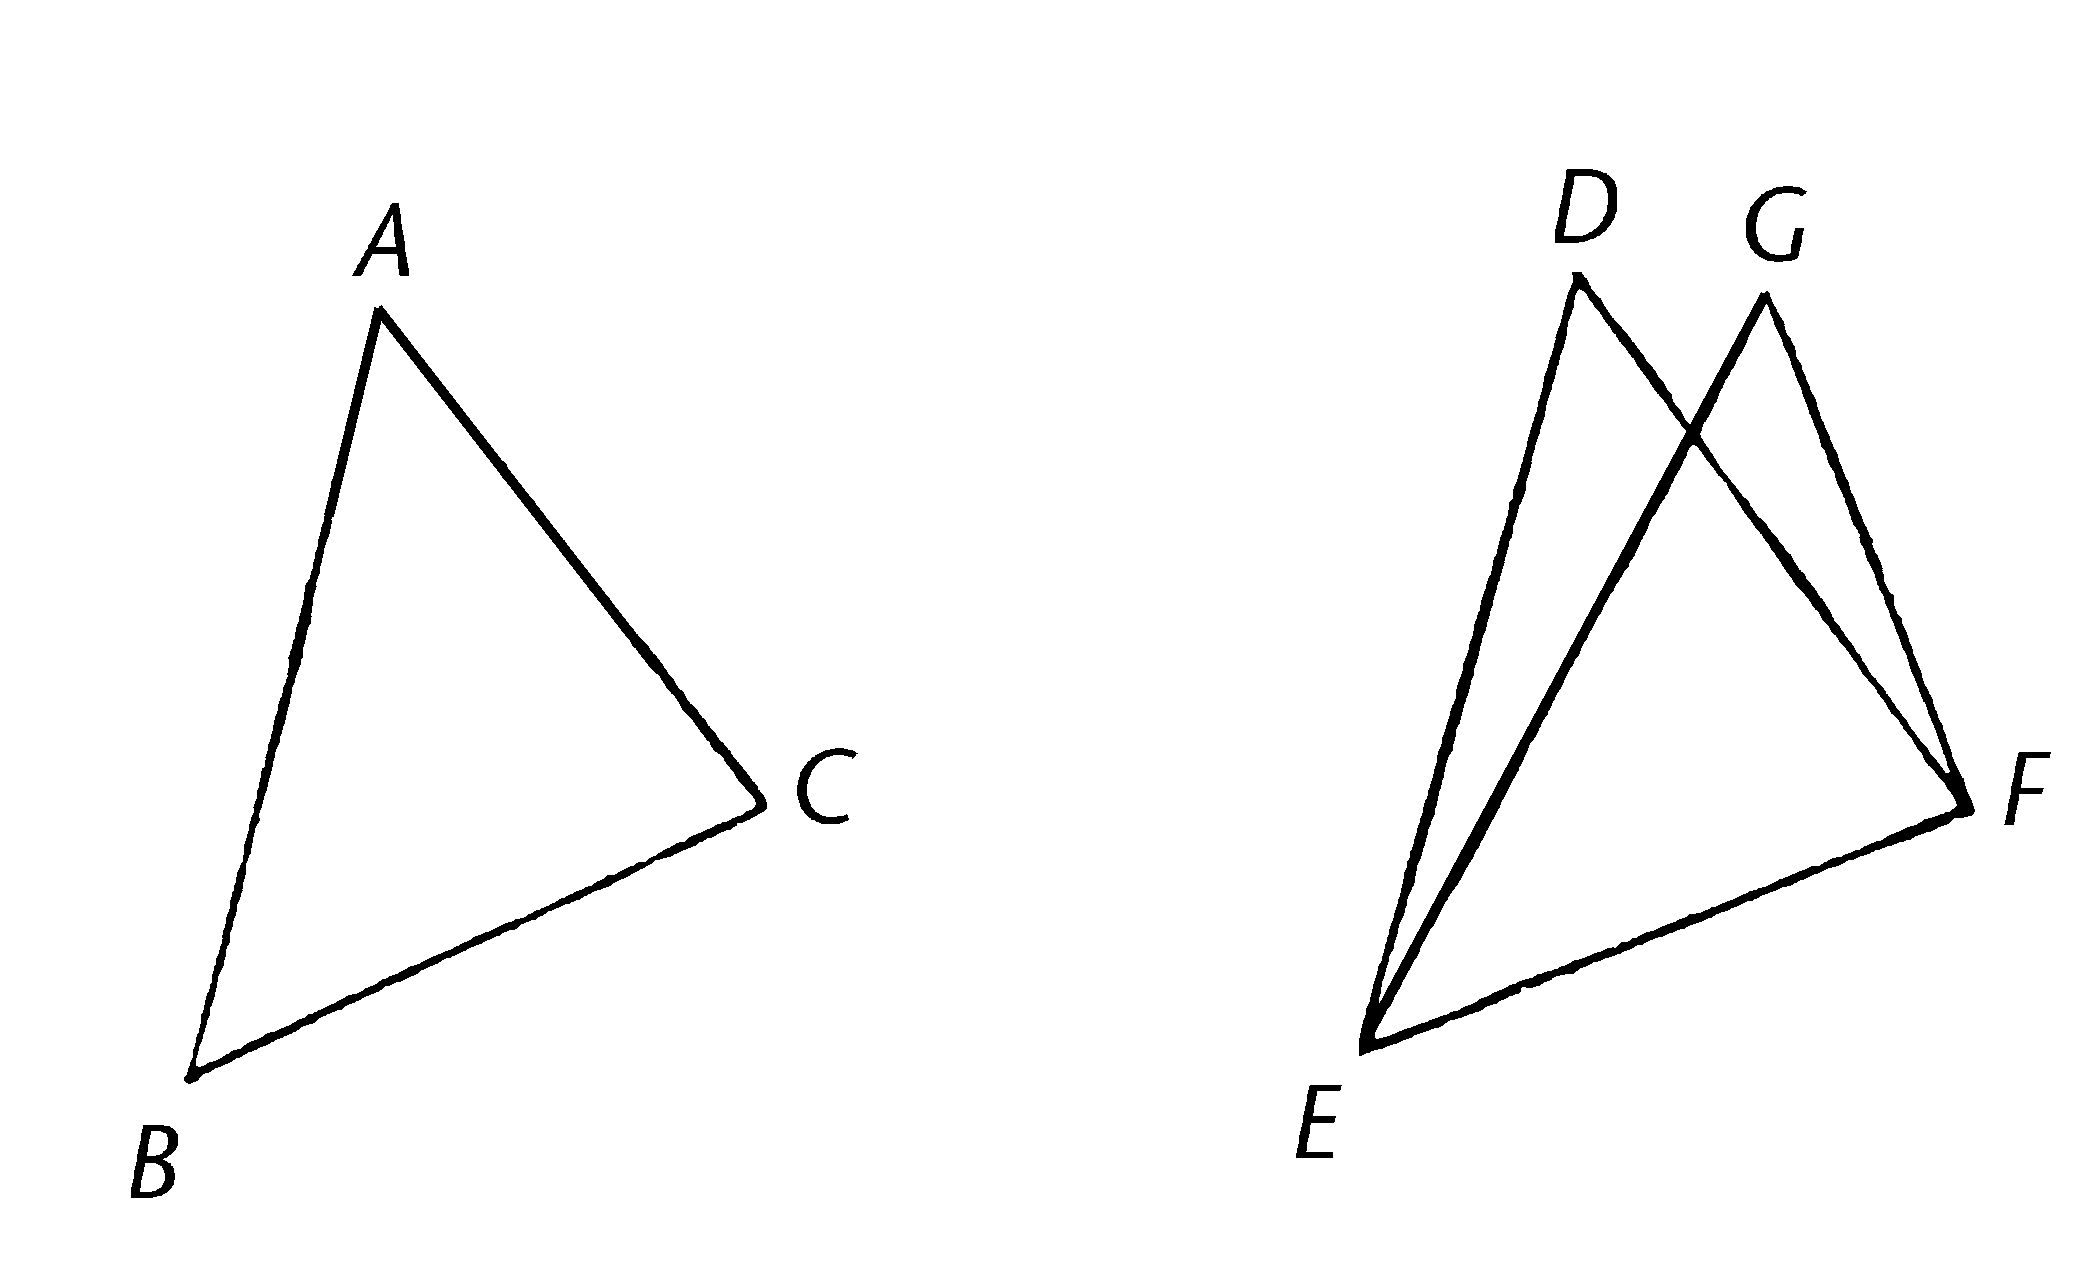
\includegraphics[width=0.5\linewidth]{./image/img464}

设三角形ABC,DEF分别有两边AB,AC等于DE,DF,其中AB等于DE,AC等于DF;并且设底边BC等于底边EF;我说角BAC等于角EDF。

因为,如果三角形ABC放置到三角形DEF,如果点B被放到点E,且直线BC到EF,点C也会与F重合,因为BC等于EF。

那么,BC重合于EF,BA,AC也重合于ED,DF;因为,如果底边BC重合于底边EF,并且边BA,AC不重合于ED,DF却像EG,GF一样落于一旁,那么,在同一条直线(由它的两端点),构建会在同一点相交的给定两线段,那在同一条直线上(由两端点),在同一侧,构建出了交于另一点的另两条线段,使之与之前的两线段相等,即分别到每个端点的线段。

但是两线段不能被如此构建。【I.7】

所以,如果底边BC放置到底边EF上,边BA,AC不重合于ED,DF,这是不可能的;所以他们重合,角BAC也重合于角EDF,并且互等。

如果,综上所述\ldots{}

Q.E.D.

问题示例:

\begin{itemize}
\tightlist
\item
  与命题I.4不同的是,I.8并没有以一个明确的陈述两三角形全等来结尾。我们应该想要它么?你是否能看到I.4在I.8中的建立角和边的应用是如何显示三角形全等的?
\item
  我们是否感觉到了欧几里得相较于无懈可击的像机器一样的公理系统的不同方法?是因为欧几里得认为他的读者是人类所以不需要点每个i和划每个t么?**
\item
  你是否掌握了证明中关于叠合的线索?叠合的三角形是那些所有对应的边和角都相等的(由此可推它们面积也相等)。叠合的三角形也是未来证明中构建块的关键,但随着我们继续开发这个架构,似乎任意等边和等角都会使得三角形叠合。到目前,关于叠合的证明我们有哪些?使用速记键,譬如SAS(边角边)或SSS(边边边)会有所帮助。
\item
  此证明与I.4所运用的策略有什么共同之处么?
\end{itemize}

\hypertarget{ux547dux9898ux4e5d}{%
\section{命题九}\label{ux547dux9898ux4e5d}}

\textbf{将给定的直线角平分。}

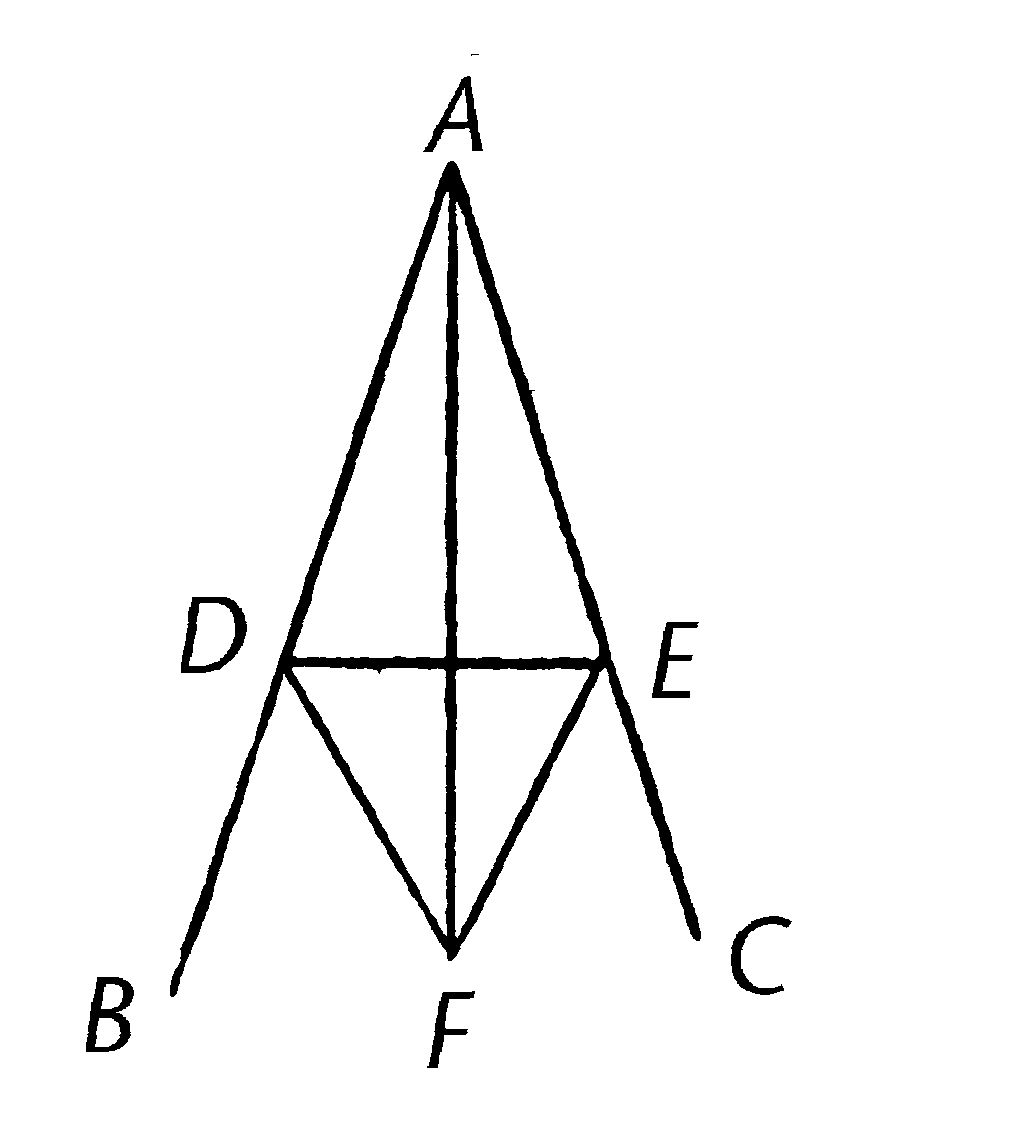
\includegraphics[width=0.3\linewidth]{./image/img467}

设角BAC是给定的直线角。

那么要求将它一分为二。

设在AB上随意取一点D;从AC上截取AE,使等于AD,连接DE,并且在DE上构建等边三角形DEF,连接AF。

我说角BAC被直线AF一分为二。

因为AD等于AE, 且AF是共有的,那么两条边DA,AF分别等于两边EA,AF。

并且底边DF等于底边EF;所以角DAF等于角EAF。

所以给定的直线角BAC被直线AF一分为二。

Q.E.F.

问题示例:

\begin{itemize}
\tightlist
\item
  在这里我们将一个角平分,在下一个命题里,我们会将一条直线平分。你会期望线的分割线更容易么?在欧几里得建造的体系中,哪一部分要求平分角被首先展示出来?
\item
  比较古希腊语\ldots\ldots.在定义17中的运用,也就是直径将圆平分(或一分为二)。那儿我们质疑断言的权威性,即翻译``平分''隐含着将圆切割成相等部分。这儿平分的意图则是毫无异议的,并且结果也确实被合理地论证了。
\item
  为什么欧几里得没有定义``平分''?一部分等于另一部分就足够了么,还是一定要说这些部分能够构成一个整体?许多事物看起来并不清晰,这是个问题么?还是说我们完全知道将一个整体切成两相等部分的含义就已经足够好了?
\end{itemize}

\hypertarget{ux547dux9898ux5341}{%
\section{命题十}\label{ux547dux9898ux5341}}

\textbf{将给定的线段平分。}

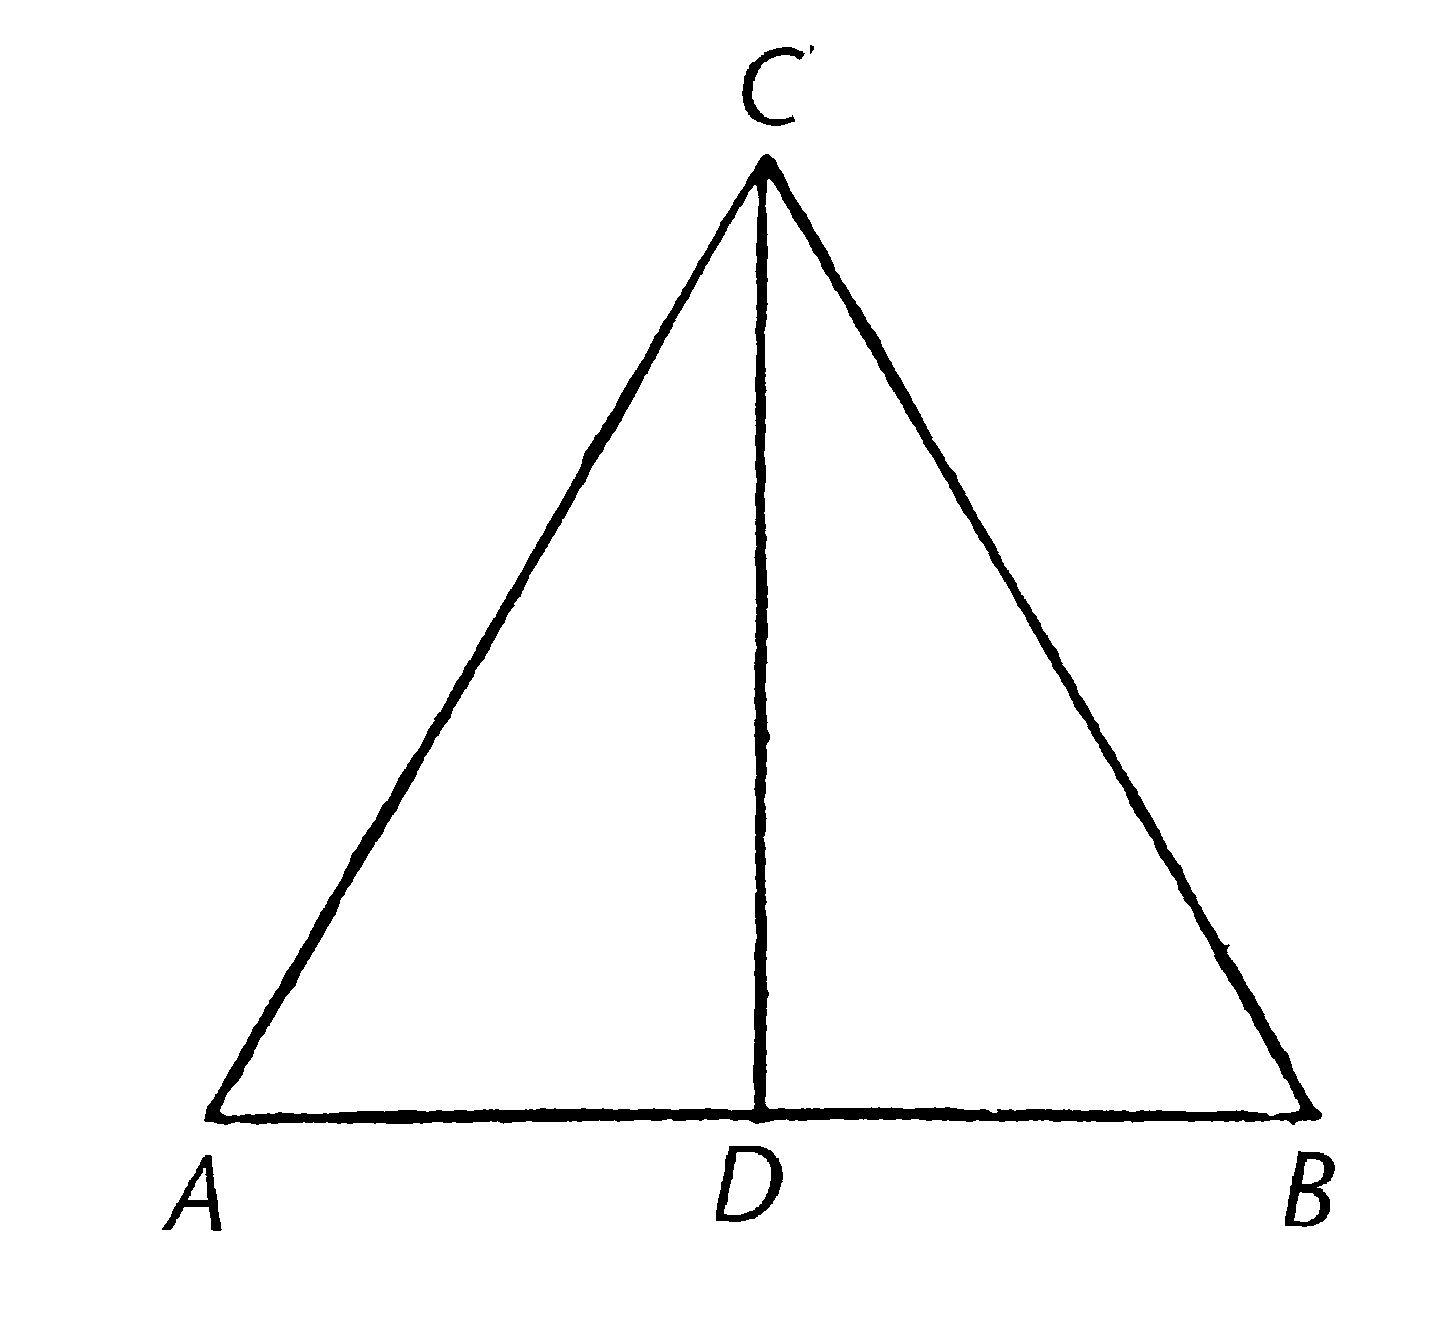
\includegraphics[width=0.3\linewidth]{./image/img469}

设AB是给定的线段。

所以要求是将线段AB平分。

在其上做等边三角形ABC【I.1】并让角ACB被直线CD平分【I.9】我说直线AB在点D被平分。

因为AC等于CB,且CD是公有的,两边AC,CD分别各自等于两边BC,CD;且角ACD等于角BCD;所以底边AD等于底边BD。【I.4】

所以给定的线段AB被平分在D。

Q.E.F.

问题示例:

\begin{itemize}
\tightlist
\item
  我们是否知道平分一条线是可能的?这是否将我们带回之前关于第一和第二条定义的问题?线是没有宽度的长度,但这是由何构成?如果这是由那些特别小的不可分割的微量构成,那么一条由奇数个微量构成的直线是不能被一分为二的。能被一分为二这个特性告诉了我们关于线的什么本质呢?
\item
  欧几里得有将部分论证与图像交流么?或许关于平分的想法?所有事物都可以口头表达么?绘画是表达你想法重要一面的正当方法么?有的人会说``口头表达和绘画都仅仅是帮助我们思考的工具。但是我们没有在思考言语或者图像。''你认为这样的说法正确么?
\item
  这些事物和自然世界的关系是怎样的?假设你正在用几何的命题划分田野。在言语和绘画的基础上,这些应用能作为第三个工具么?这个范例能帮助我们思考数学的理想化么?它能帮我们提升前文中讨论到的柏拉图分割线么?
\end{itemize}

\hypertarget{ux547dux9898ux5341ux4e00}{%
\section{命题十一}\label{ux547dux9898ux5341ux4e00}}

\textbf{在给定直线的给定点上,画一直线与给定直线呈直角。}

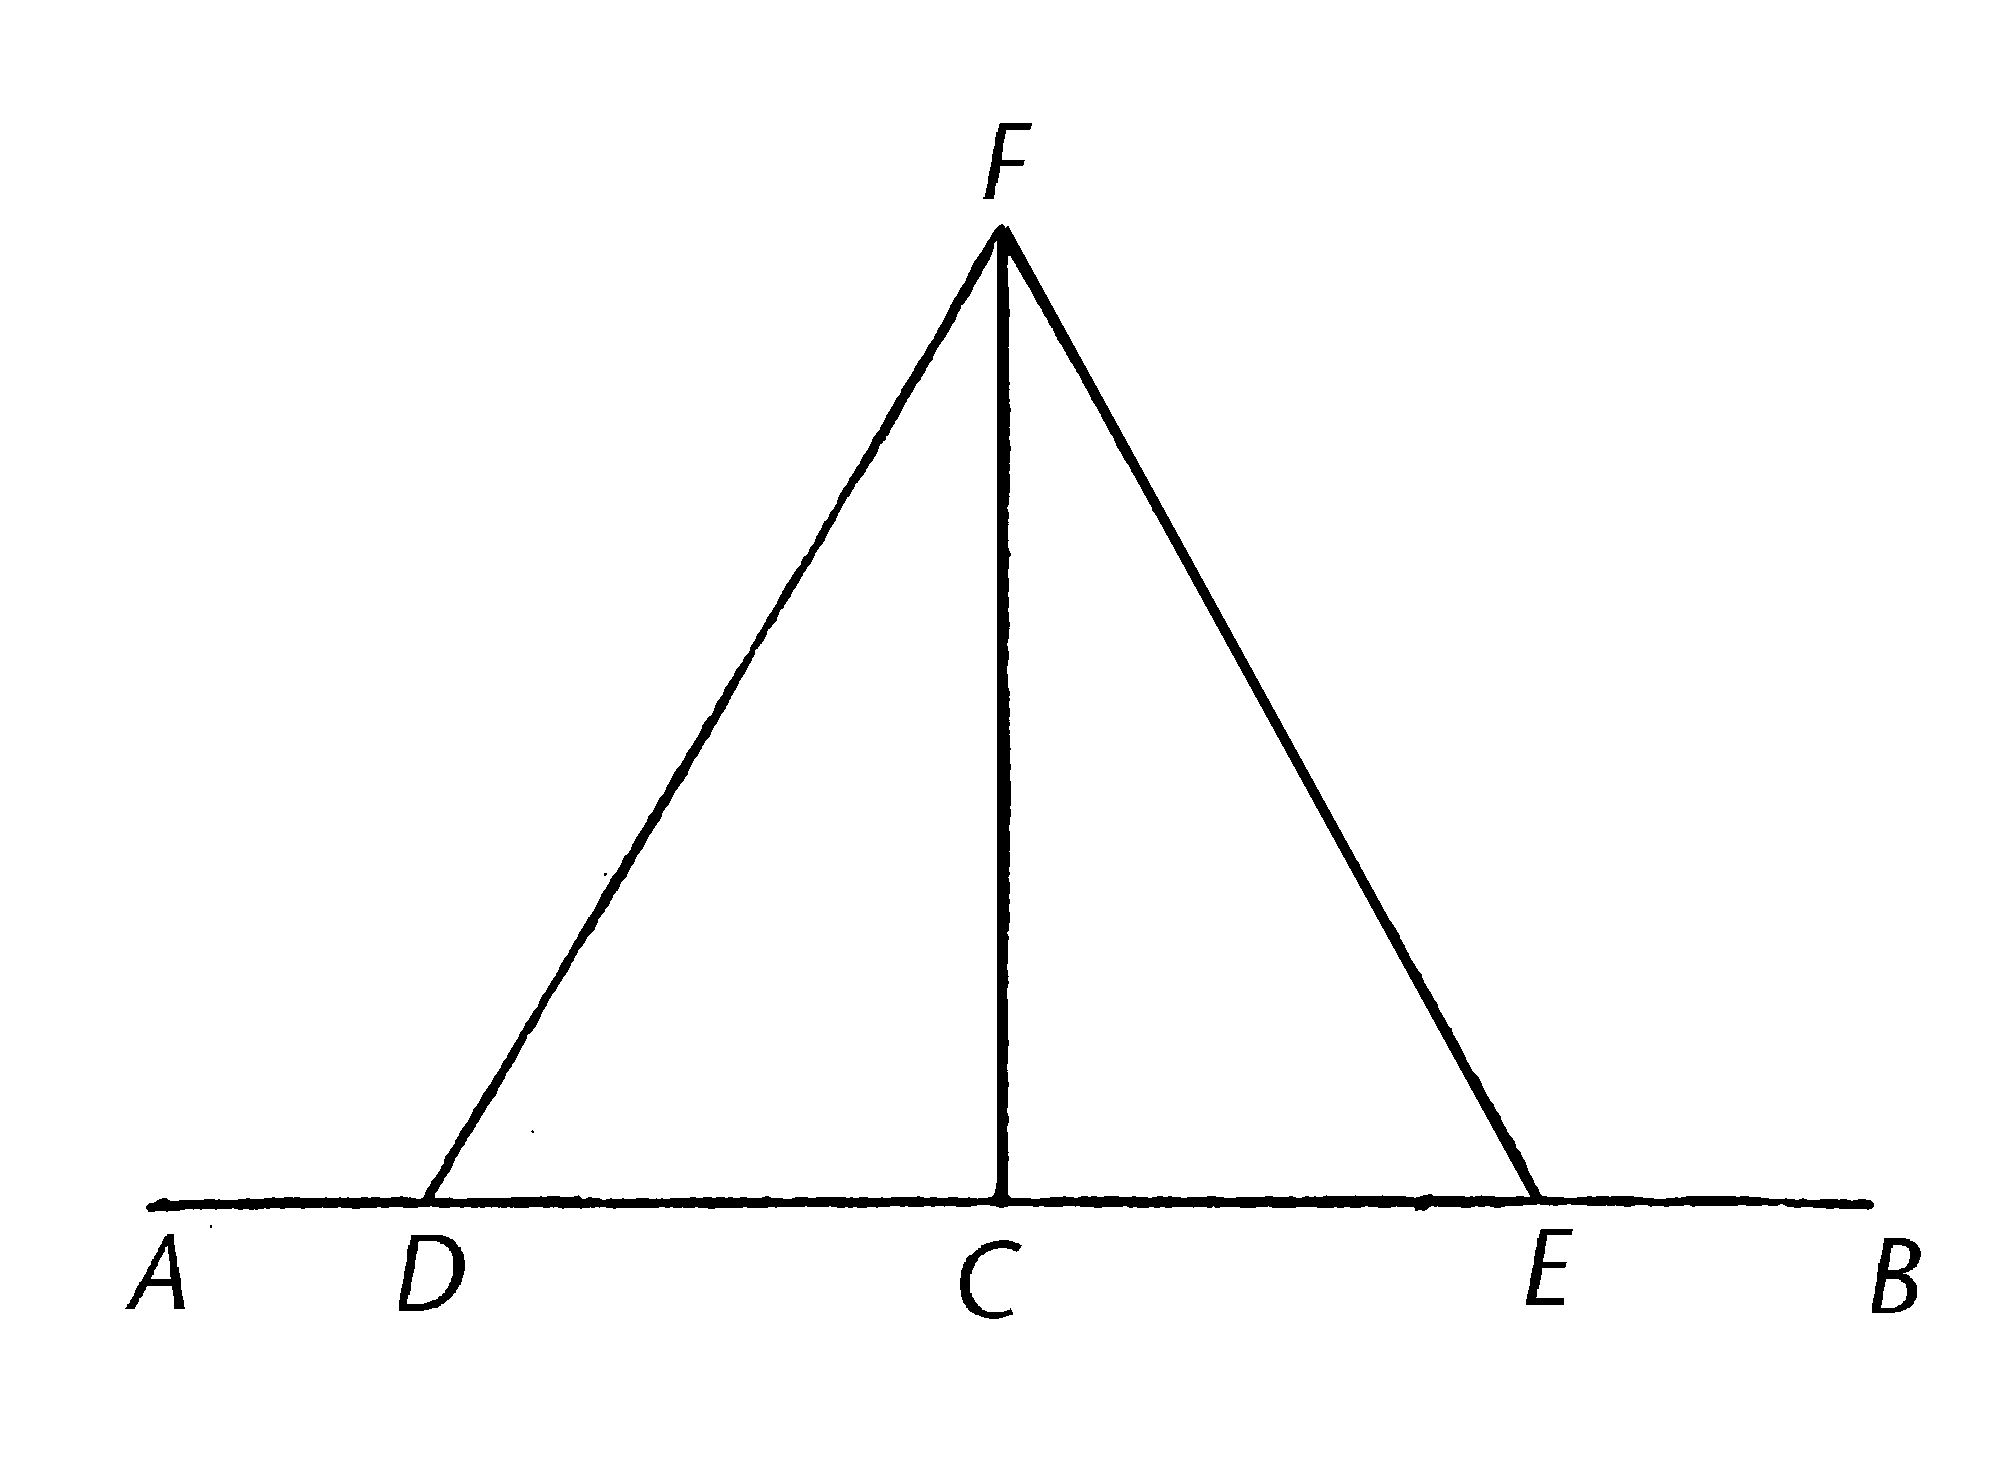
\includegraphics[width=0.4\linewidth]{./image/img471}

设AB为给定直线,且C是其上一给定点。

所以要求从点C画一直线与直线AB呈直角。

在AC上设任意一点D;作CE使等于CD;【I.3】在DE上构建等边三角形FDE,【I.1】并且连接FC;我说直线FC与给定的直线AB呈直角且起于给定点C。

因为DC等于CE,并且CF是公有的,两边DC,CF各自与两边EC,CF互等;且底边DF等于底边FE;所以角DCF等于角ECF; 【I.8】且他们是相邻角。

但当一条直线置于另一条直线上,并使得两个相邻角互等,每个角都是直角;【定义十】所以DCF,FCE都是直角。

所以在给定直线AB的给定点C上作的直线CF与AB呈直角。

Q.E.F.

\hypertarget{ux547dux9898ux5341ux4e8c}{%
\section{命题十二}\label{ux547dux9898ux5341ux4e8c}}

\textbf{给定一无限直线,在线外一给定点上,画垂线。}

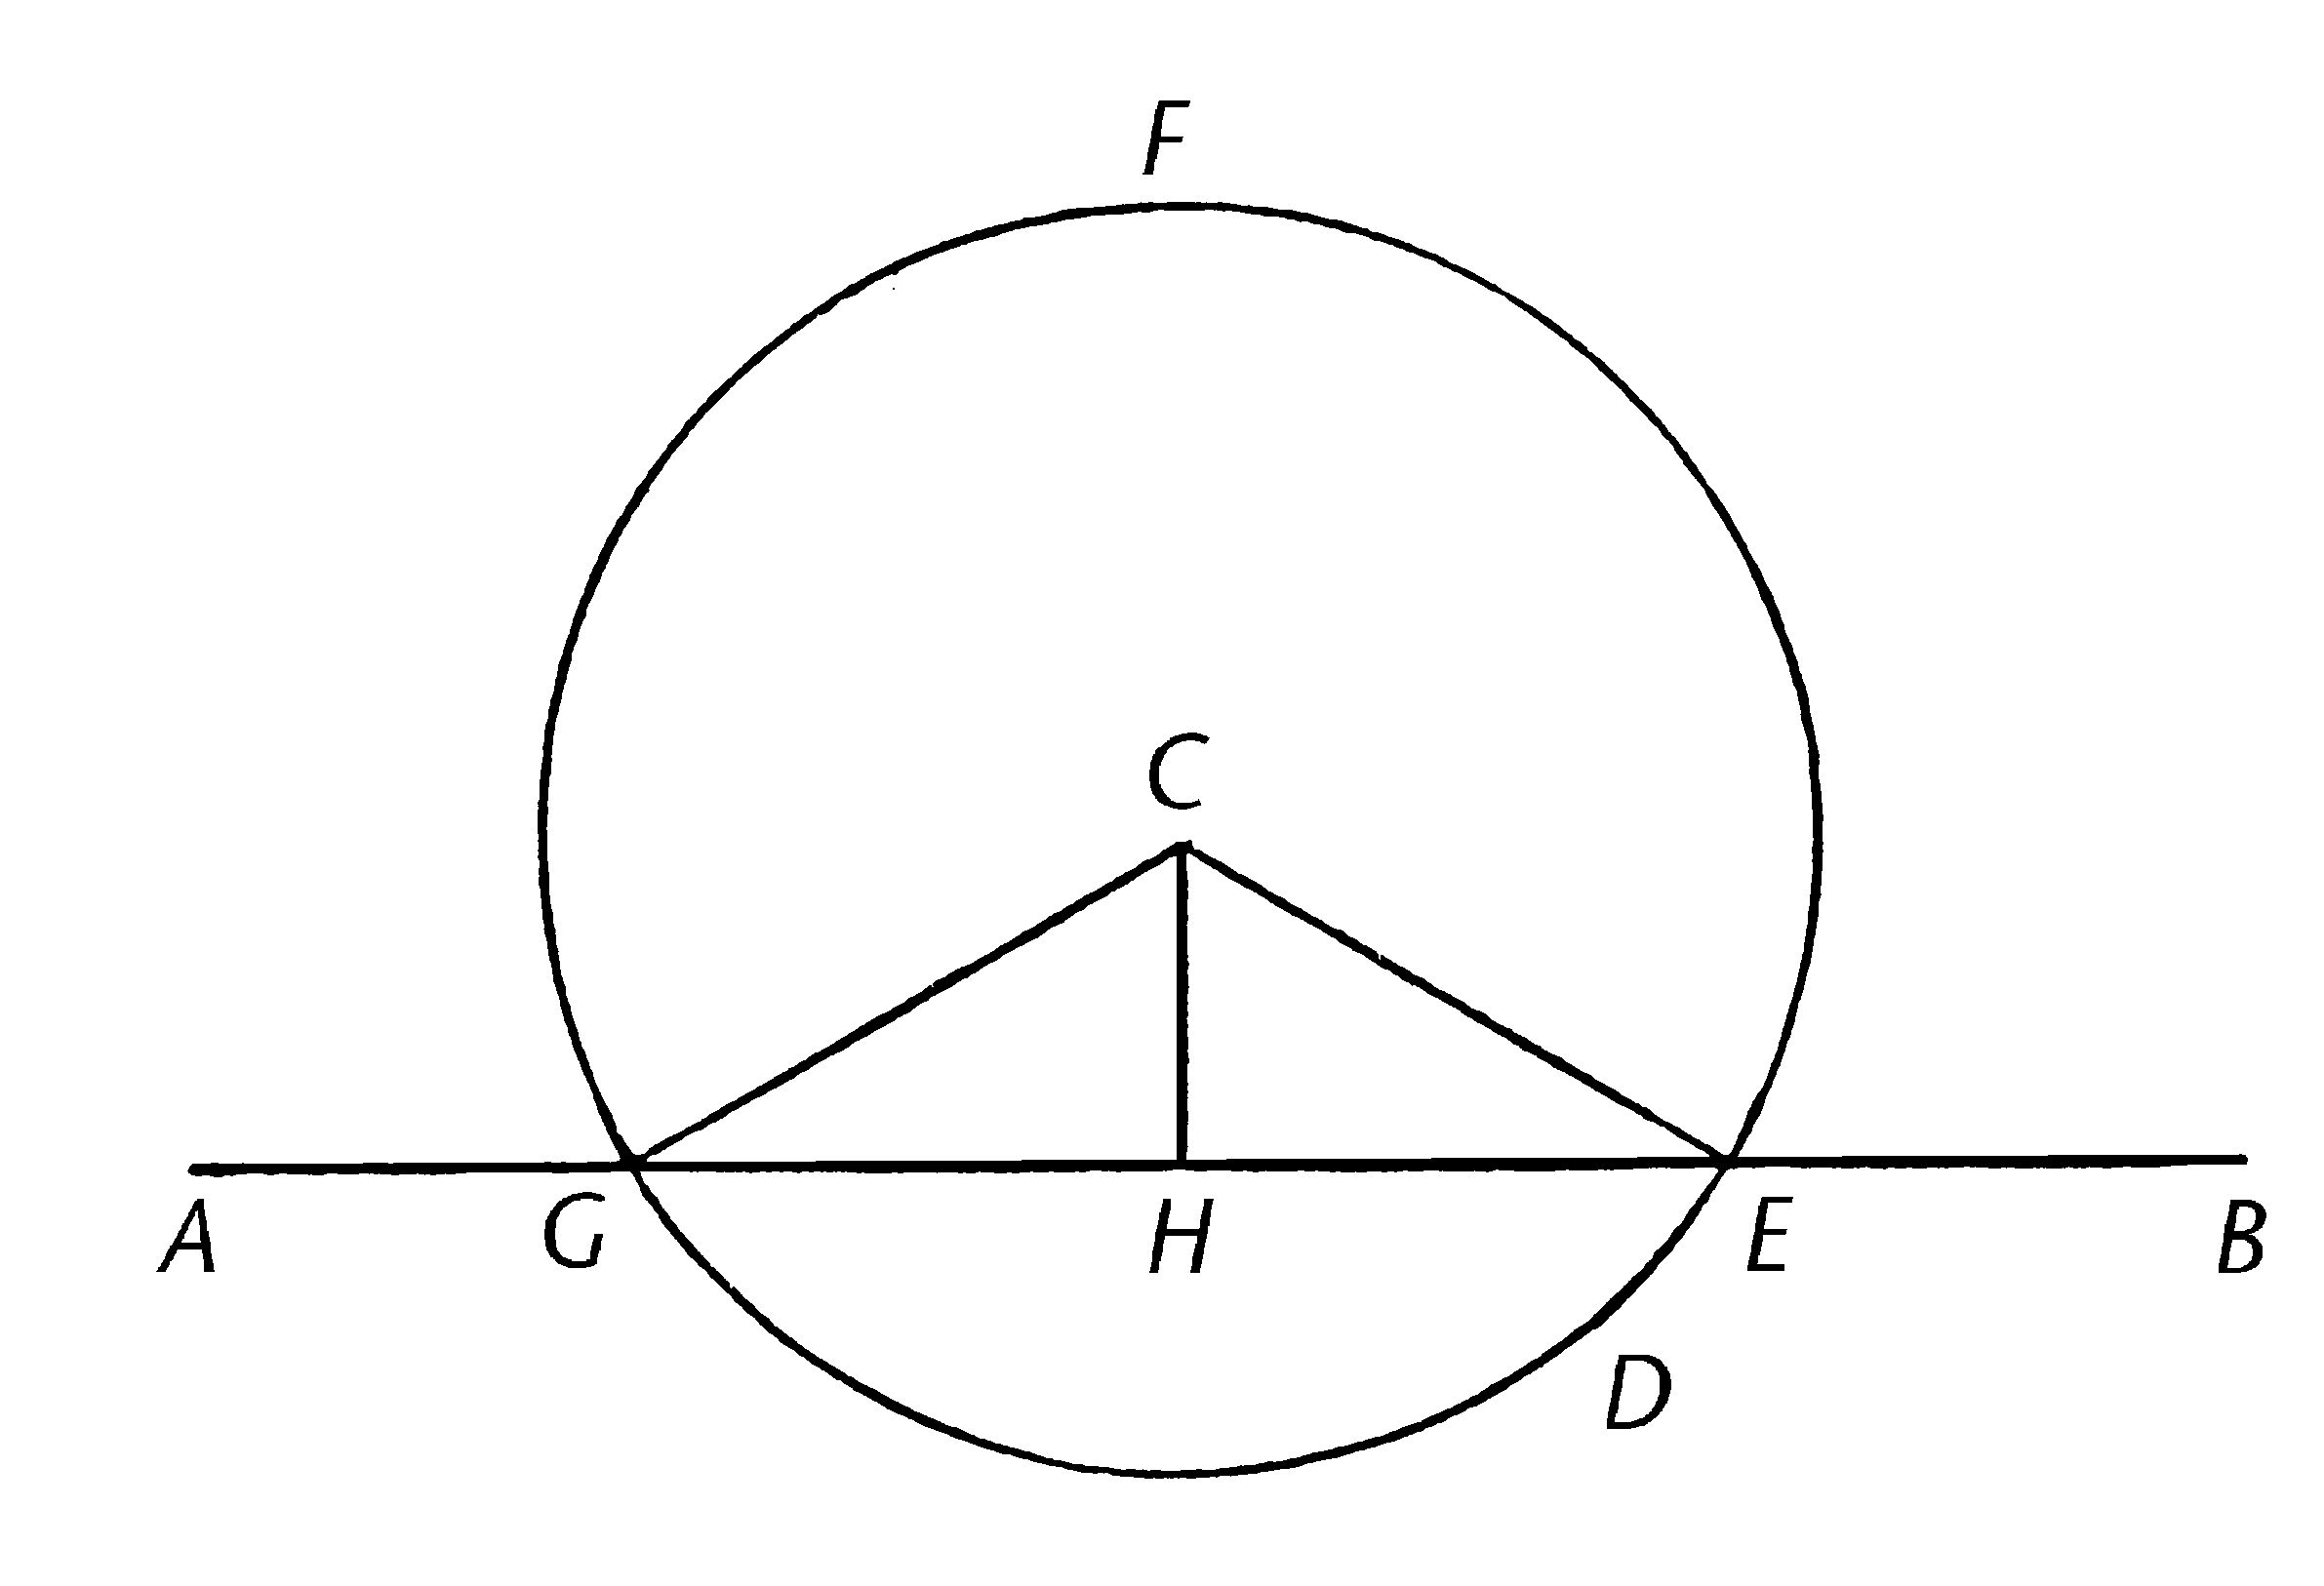
\includegraphics[width=0.4\linewidth]{./image/img473}

设AB是给定的无限直线,C是线外的一点;所以要求是在给定的无限直线AB外的C上画垂线。

在AB的另一侧取任意一点D,并以C为圆心,CD为距离,画圆EFD;【公设3】在H平分直线EG,【I.10】并连接直线CG,CH,CE。【公设1】

我说CH是由给定无限直线AB外的C上所画垂线。

因为GH等于HE, 且HC是公有的,两条边GH,HC各自与两边EH,HC互等;且底边CG等于底边CE;所以角CHG等于角EHC。【I.8】

并且他们是相邻角。

但是,当一条直线置于另一条直线上,并使得两个相邻角互等,每个角都是直角,置于另一条直线上的这条直线被称为垂直于另一条直线。【定义10】

所以CH是由给定无限直线AB外的C上所画垂线。

Q.E.F.

问题示例:

\begin{itemize}
\tightlist
\item
  为什么线必须是无限的?在这里无限的含义是什么?
\end{itemize}

\hypertarget{ux547dux9898ux5341ux4e09}{%
\section{命题十三}\label{ux547dux9898ux5341ux4e09}}

\textbf{如果将一条直线置于另一条直线上成夹角,要么成两直角,要么与两直角相等。}

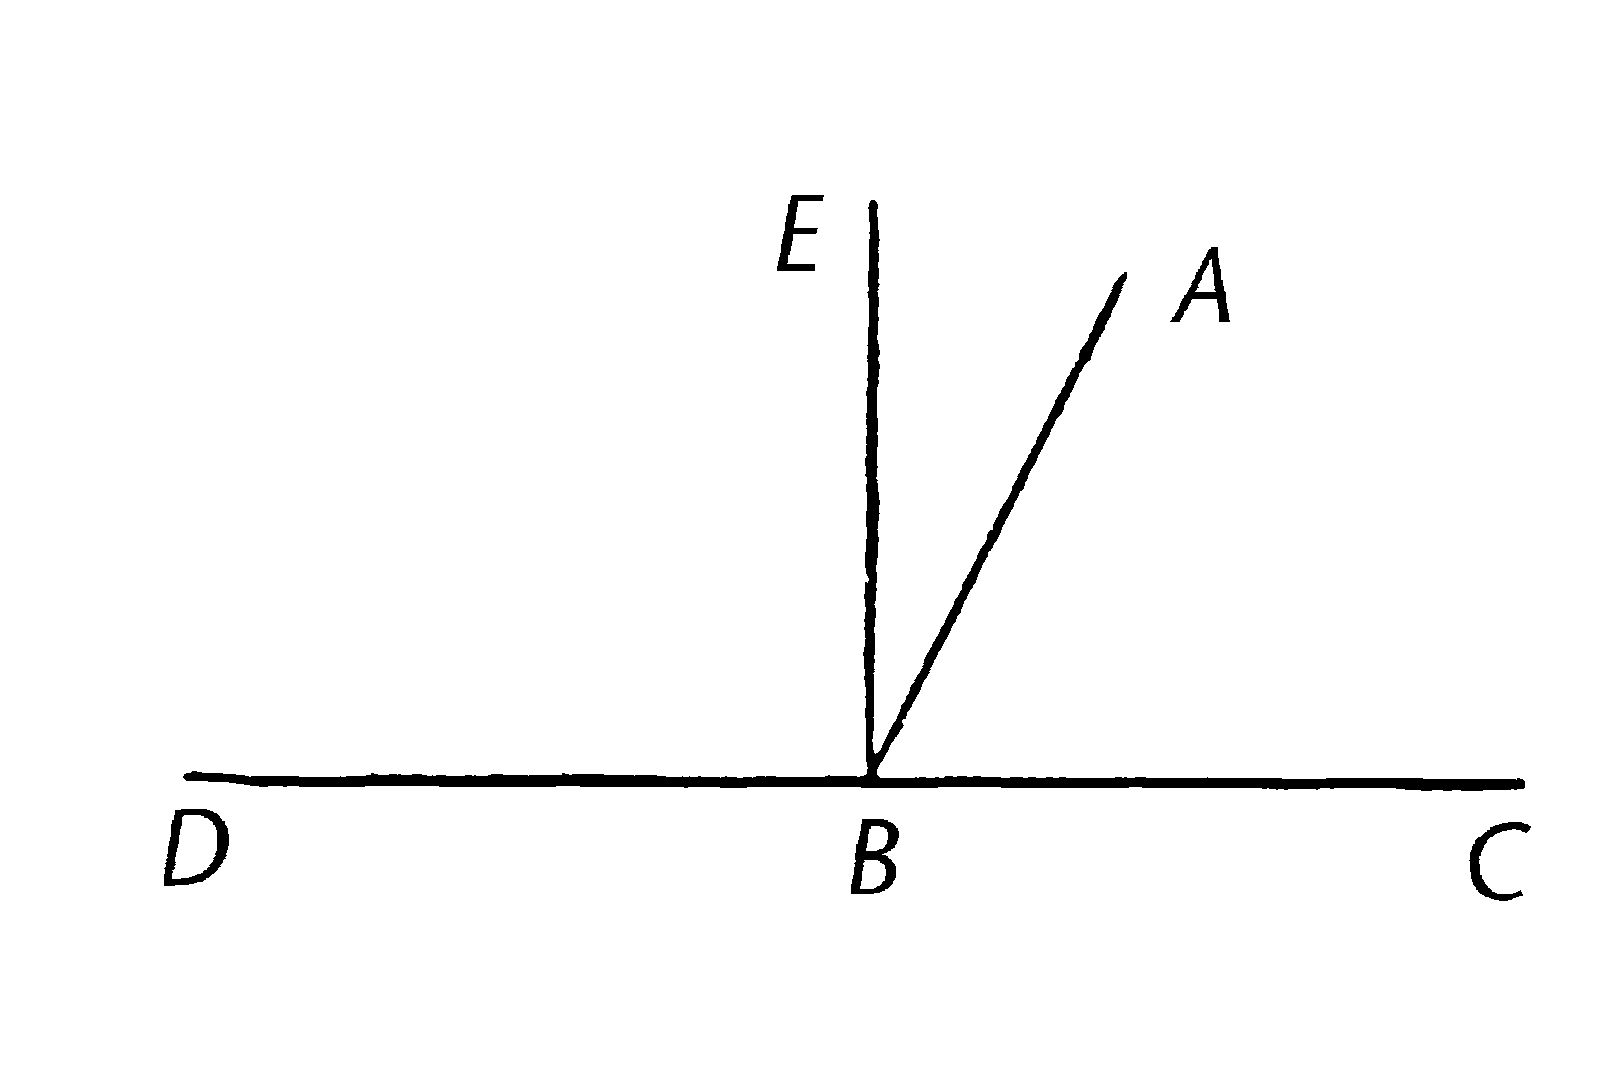
\includegraphics[width=0.4\linewidth]{./image/img475}

对于设直线AB在CD上成夹角CBA,ABD; 我说角CBA,ABD或者是两直角,或者等于两个直角。

现在,如果角CBA等于角ABD,他们是两个直角;【定义10】

但是,如果不是的话,从点B画BE与CD成直角。【I.11】所以角CBE,EBD是两直角。

那么,因为角CBE与角CBA,ABE相等,再各自加上角EBD;所以角CBE,EBD与三个角CBA,ABE,ECD相等。【公理2】

再一次,因为角DBA与角DBE,EBA相等,再各自加上角ABC;所以角DBA,ABC与三个角DBE,EBA,ABC相等。【公理2】

但是,角CBE,EBD已被证明相等于同样的三个角;且与同一事物相等的事物们彼此互等;【公理1】所以角CBE,EBD也等于角DBA,ABC。

但是角CBE,EBD是两个直角;所以角DBA,ABC也等于两个直角。

综上所述\ldots{}

Q.E.D.

问题示例:

\begin{itemize}
\tightlist
\item
  这儿是对定义十的应用:因为我们证明了角是相等的,通过定义十我们知道有两个直角。那儿我们说了这是我们将称为直角的角。(当我们仔细考虑公设4的时候,需要重新思考这一点。)现在当我们应用在这个命题时,看起来合理么?
\end{itemize}

\hypertarget{ux547dux9898ux5341ux56db}{%
\section{命题十四}\label{ux547dux9898ux5341ux56db}}

\textbf{如果在任意直线的一点上,有两条直线不在同一侧,且使得所成相邻角等于两直角,则这两条直线在同一直线上。}

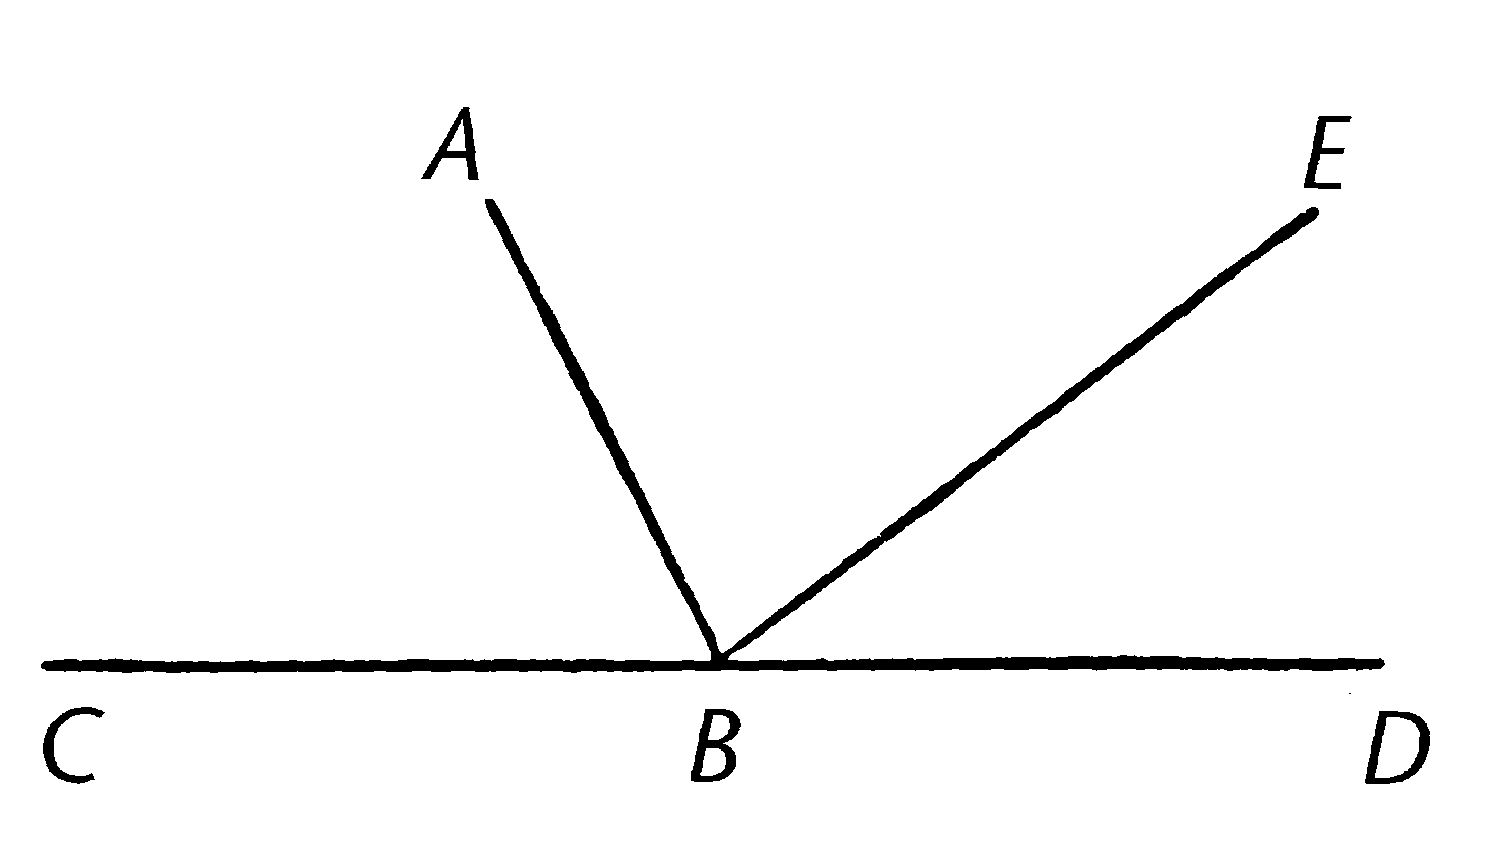
\includegraphics[width=0.4\linewidth]{./image/img477}

对于在任意直线AB上的点B,使BC,BD落在不同侧使得相邻角ABC,ABD等于两直角;我说BD和CB在同一直线上。

因为,如果BD和BC不在同一条直线上,使BE在CB在同一条线上。

那么,因为直线AB在直线CBE上,角ABC,ABE等于两直角【I.13】

但是角ABC,ABD也等于两直角;所以角CBA,ABE也等于角CBA,ABD。【公设4和公理1】

将角CBA从各自中减去;所以剩余的角ABE等于剩余的角ABD,【公理3】小的等于大的:这是不可能的。
所以BE和CB不在同一直线上。

同样地,我们可以证明除BD外,没有其它直线和CB在同一直线上。

所以CB和BD在同一直线上。

综上所述\ldots{}

Q.E.D.

问题示例:

\begin{itemize}
\tightlist
\item
  你能在不引用公设4所有直角都相等的情况下完成这个论证么?(这个问题同样适用于命题15)
\end{itemize}

\hypertarget{ux547dux9898ux5341ux4e94}{%
\section{命题十五}\label{ux547dux9898ux5341ux4e94}}

\textbf{如果两直线相交,他们所成的对顶角互等。}

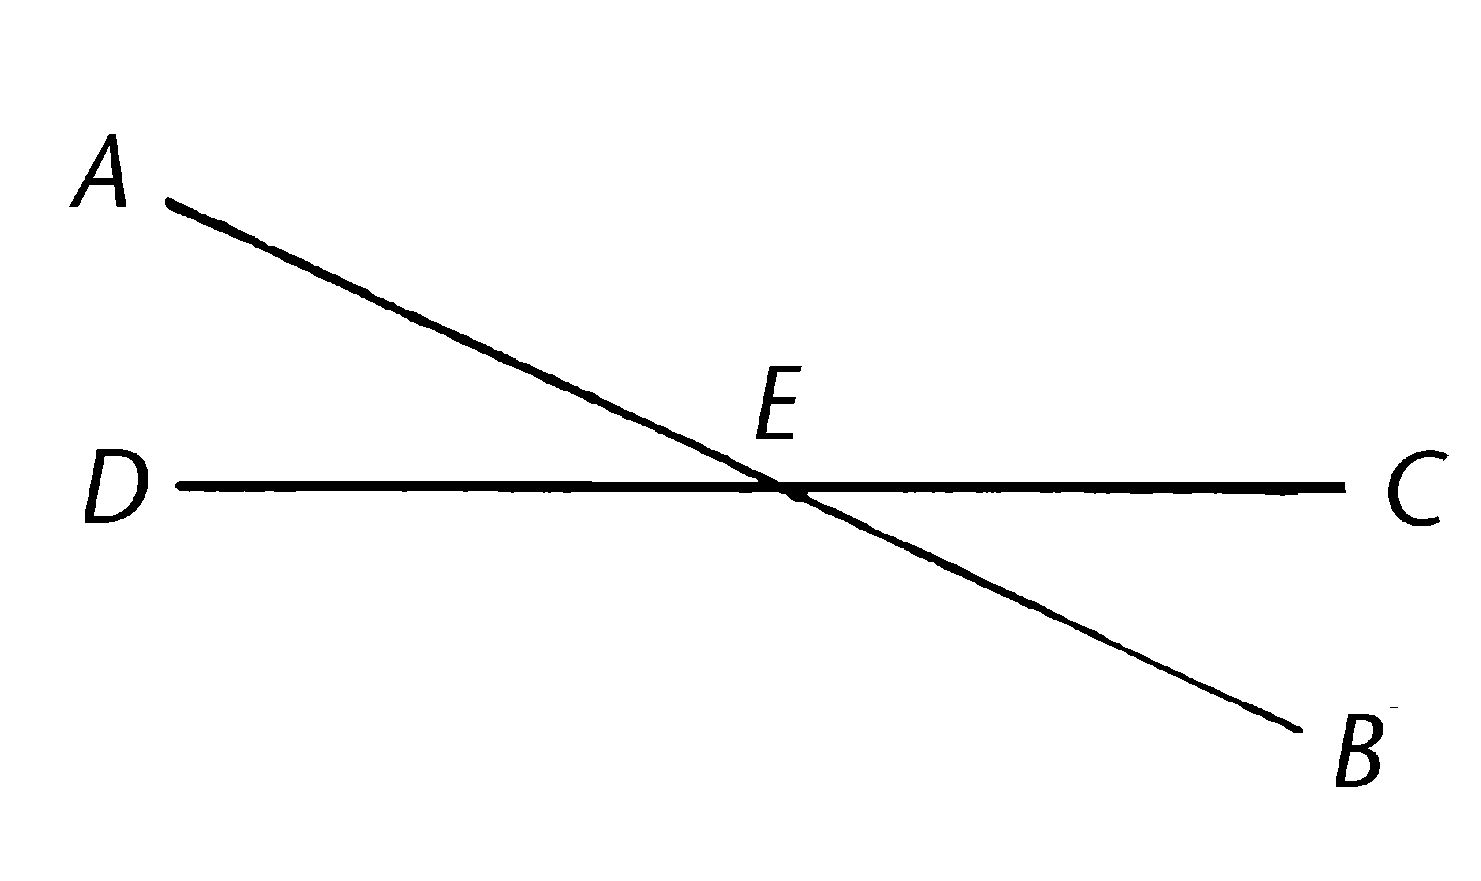
\includegraphics[width=0.4\linewidth]{./image/img479}

设直线AB,CD相交在点E;我说角AEC等于角DEB,且角CEB等于角AED。

因为直线AE在直线CD上,并成夹角CEA,AED,角CEA,AED等于两直角。【I.13】

因为直线DE在直线AB上,并成夹角AED,DEB,角AED,DEB等于两直角。【I.13】

但是角CEA,AED也已被证明与两直角相等;所以角CEA,AED等于角AED,DEB.【公设4和公理1】

将角AED从各自中减去;所以剩余的部分角CEA与BED互等。【公理3】

类似地,可以证明角CEB,DEA也互等。

综上所述\ldots{}

Q.E.D.

\textbf{推论} 「由此,显然的,如果两直线相交,它们之间在交点所成的角等于四个直角。」

编者注:在此及本书其它地方的「」用于指明被学者们认为是早期编辑文本添加的内容,也就是说非最初欧几里得给出的。其中一部分假定为添加的内容被Heath还有我们(以「」的形式)保留下来,是因为他们已经被包含在了在重要的古希腊语文本中很久,他们具有准-欧几里得的地位。现在的推论已展现在Proclus(公元410-485年)时期的手稿中。关于推论的含义,查阅\protect\hyperlink{plato}{前文}。

\hypertarget{ux547dux9898ux5341ux516d}{%
\section{命题十六}\label{ux547dux9898ux5341ux516d}}

\textbf{在任意三角形中,如果延长其中一边,那么外角大于内对角。}

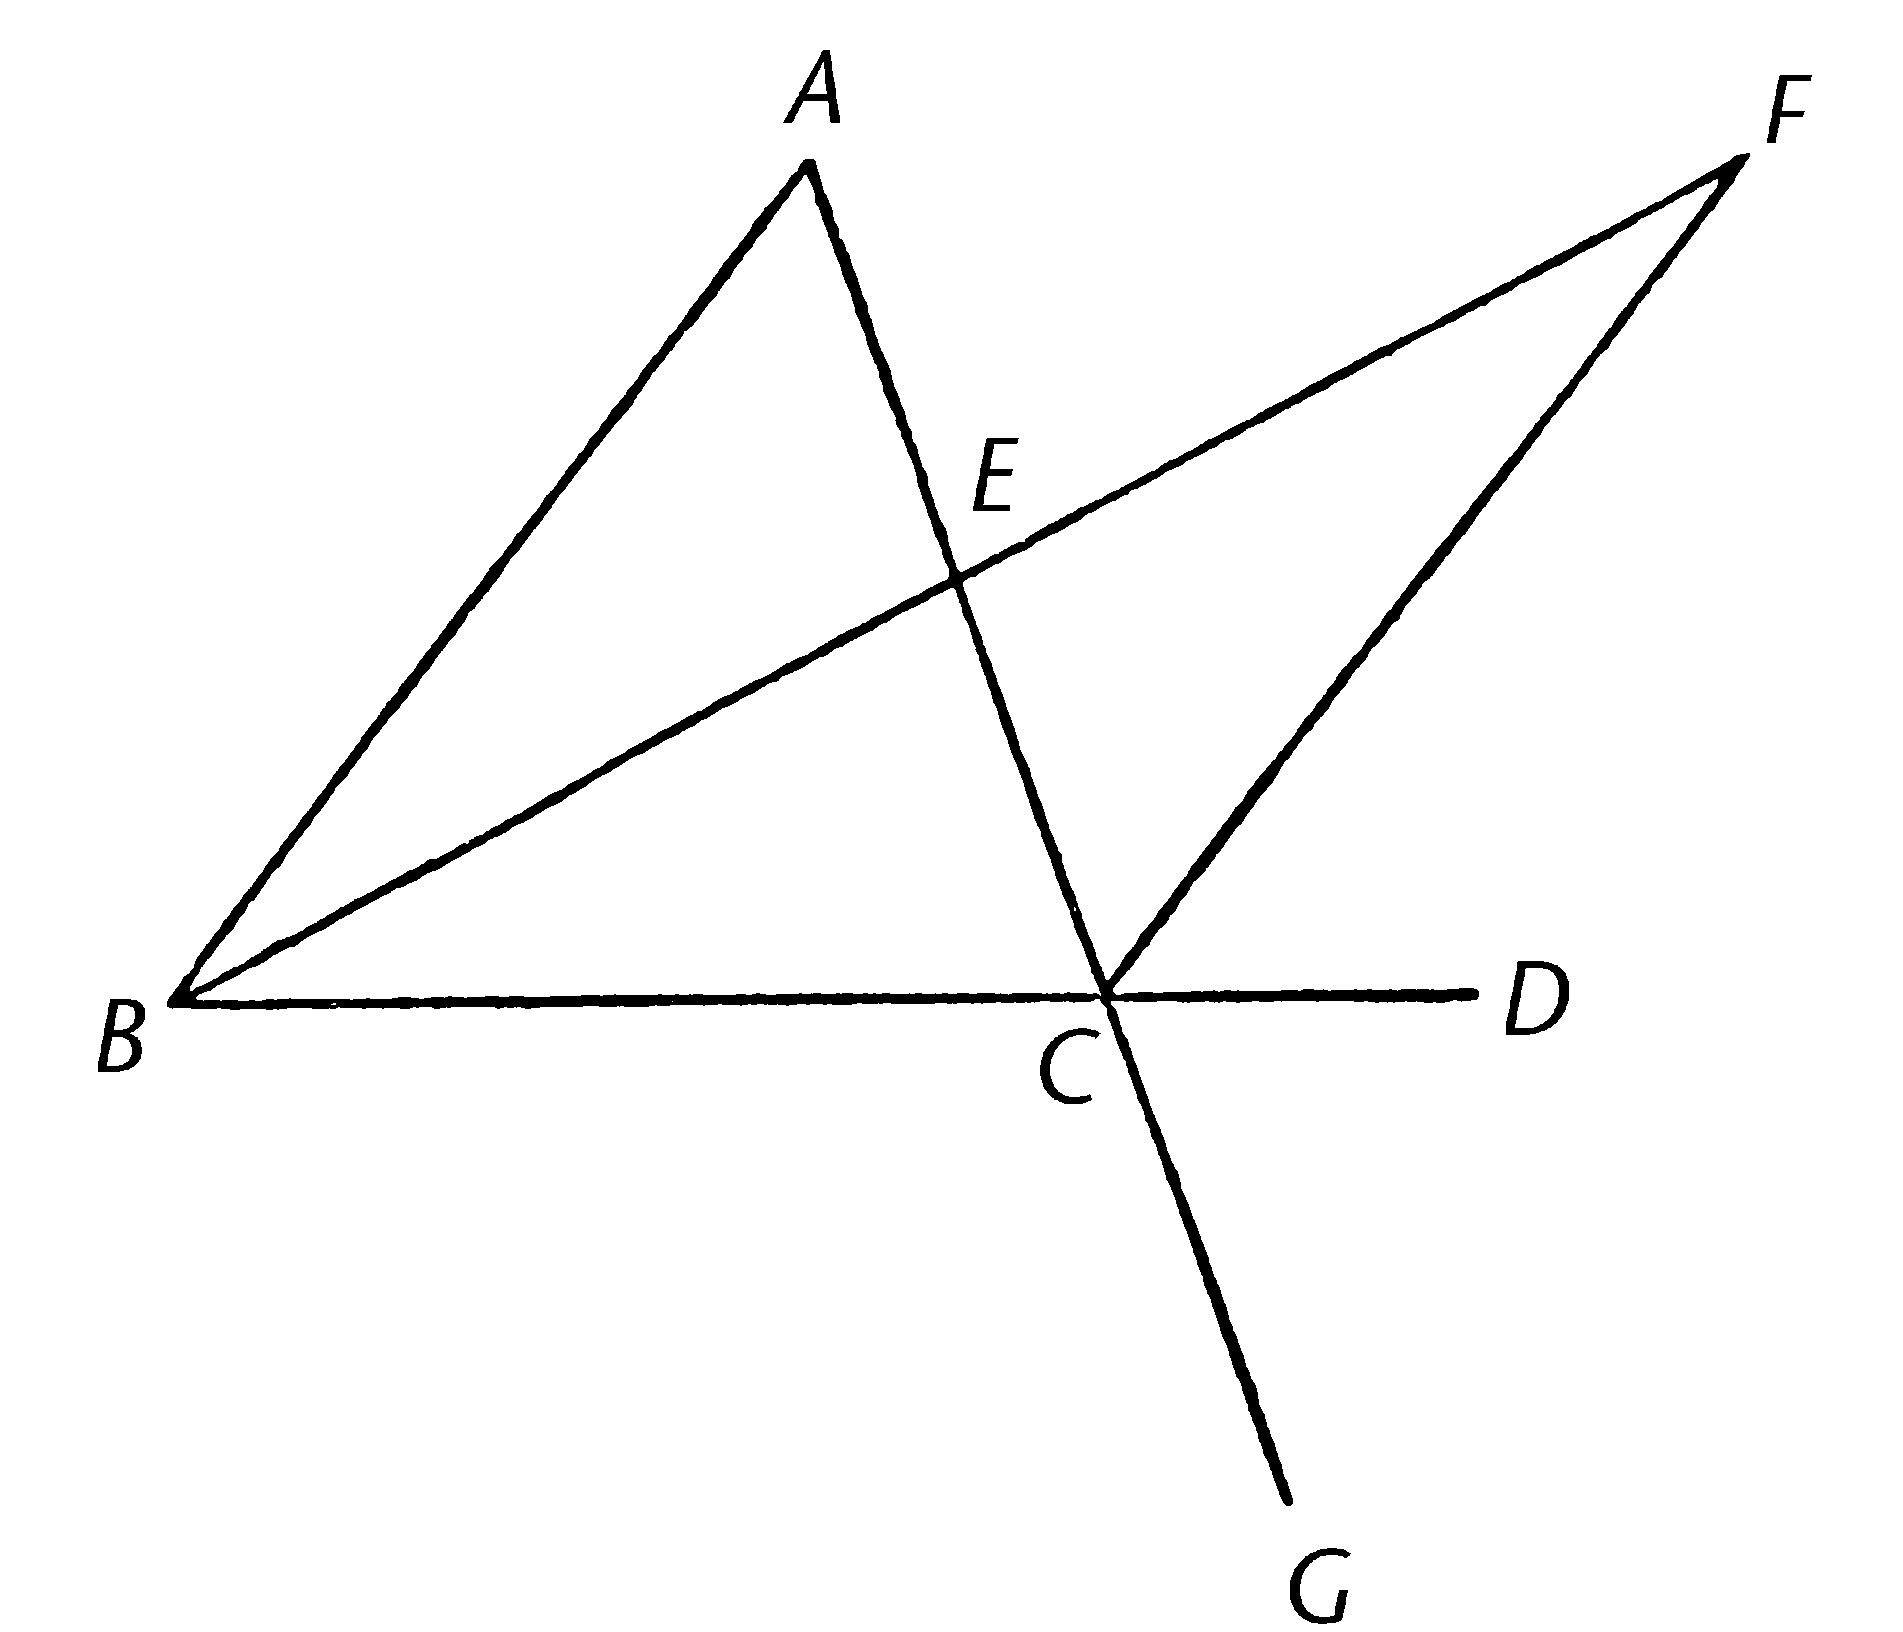
\includegraphics[width=0.3\linewidth]{./image/img481}

设ABC为三角形,并将其中一边BC延长至D;我说外角ACD大于内对角CBA和角BAC。

将AC在E平分,【I.10】并连接BE且在同一条直线上延长至F;使得EF等于BE,【I.3】连接FC,【公设1】并画AC到G。【公设2】

那么,因为AE等于EC,BE等于EF,两边AE,EB各自与两边CE,EF互等;且角AEB等于角FEC,因为它们是对顶角。【I.15】

所以底边AB等于底边FC,三角形ABE全等于三角形CFE,且剩余的各等边对应的角也各自相等;【I.4】所以角BAE等于角ECF。

但是角ECD比角ECF大;【公理5】所以角ACD大于角BAE。

类似地,如果平分BC,角BCG,也就是角ACD【I.15】可以被证明比角ABC大。

综上所述\ldots{}

Q.E.D.

问题示例:

\begin{itemize}
\tightlist
\item
  我们如何知道CF会落在角ACD以内?
\item
  你是否有注意到在搭建线和角的性质时,欧几里得有多么的仔细?现在,他从搭建的线和角中移到三角形,探讨边和角的关系。注意看他是如何发展三角形的这些特性的。你能够看到这些关系的多样性的是如何丰富的?他正在指引我们变得能够绘出关于平行线和相等面积的结论。
\end{itemize}

\hypertarget{ux547dux9898ux5341ux4e03}{%
\section{命题十七}\label{ux547dux9898ux5341ux4e03}}

\textbf{在任意三角形中,以任意方式取任意两角,其两角(之和)小于两直角。}

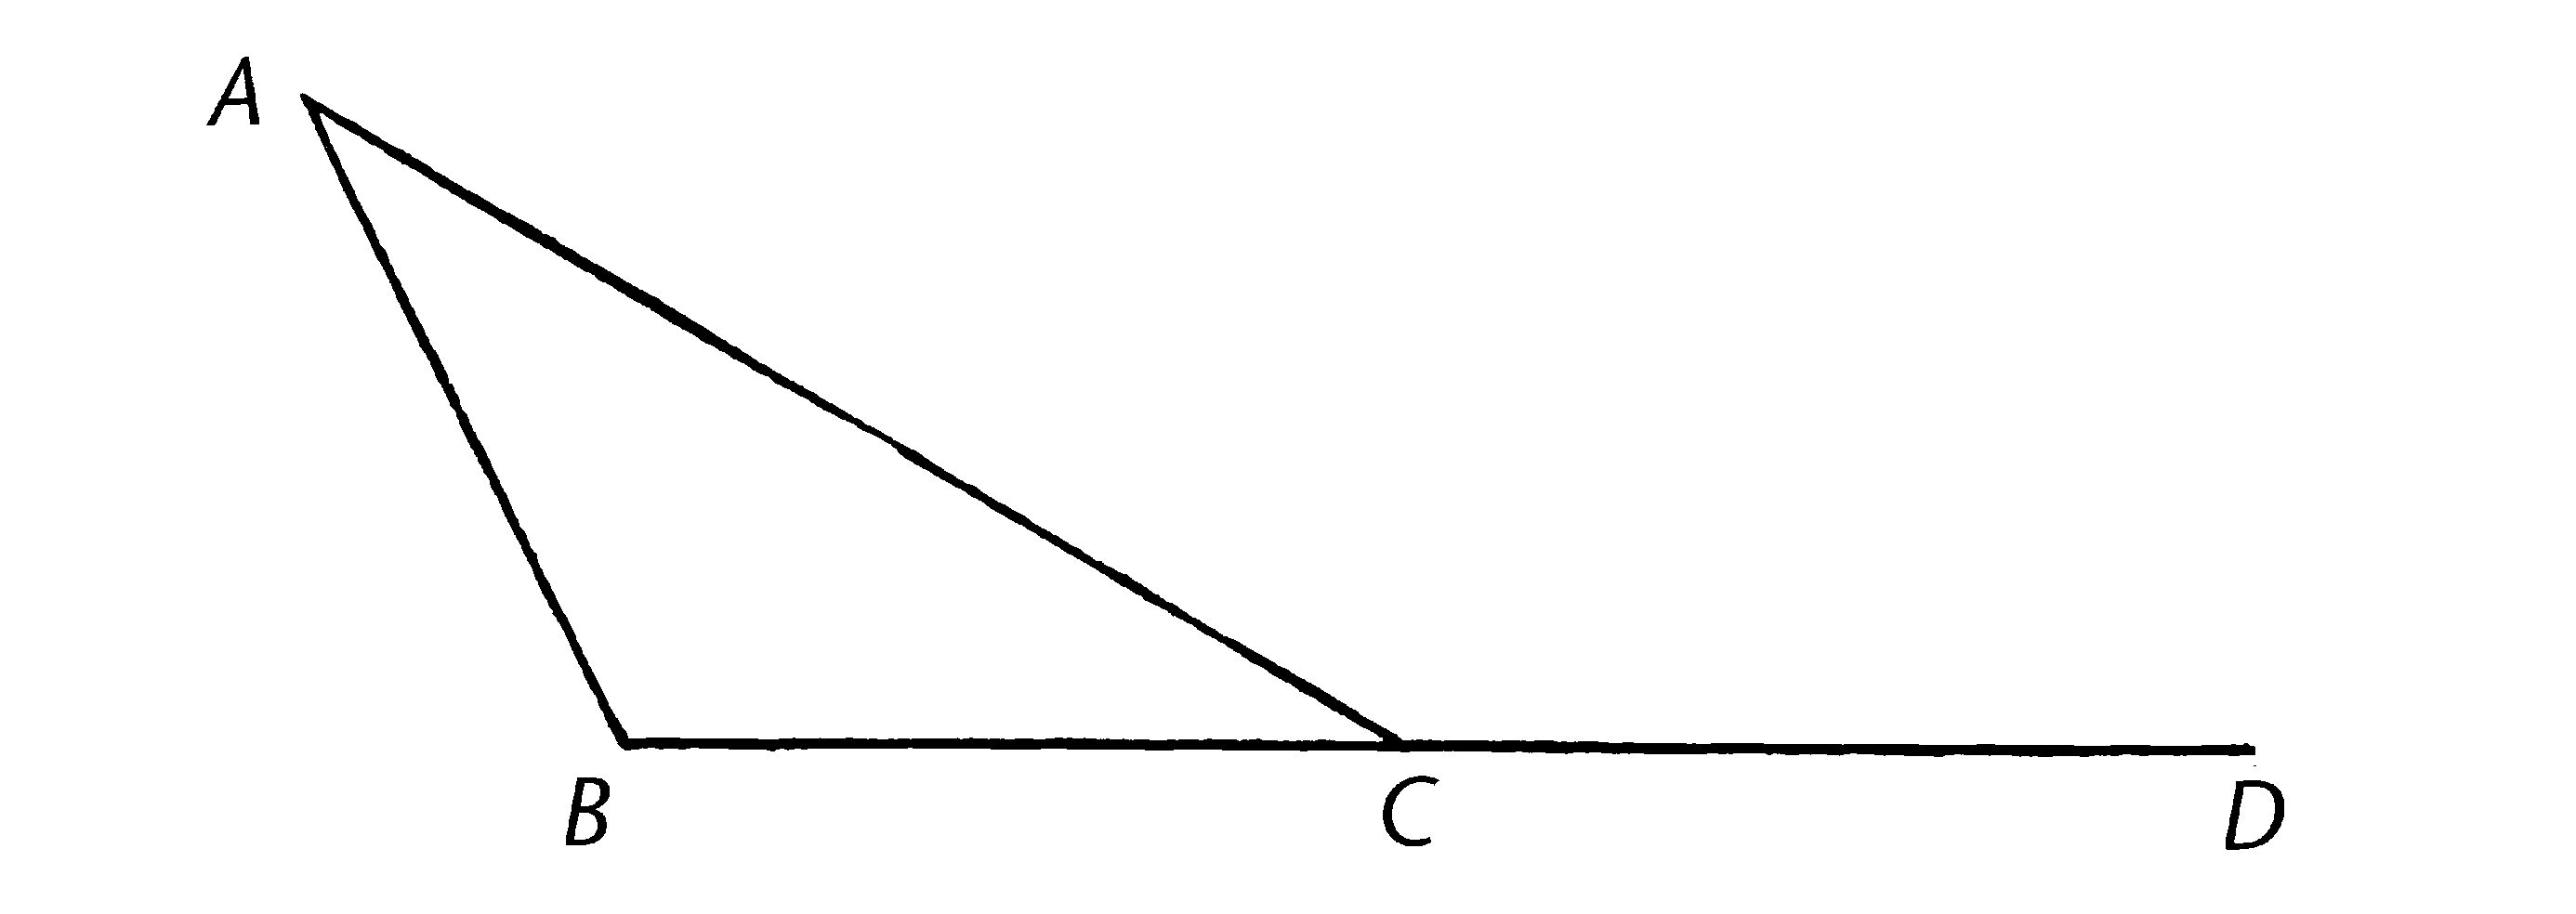
\includegraphics[width=0.5\linewidth]{./image/img483}

设ABC为三角形,我说在三角形ABC内以任意方式取任意两角,其两角(之和)小于两直角。

延长BC到D。【公理2】

那么,因为角ACD是三角形ABC的外角,它比内对角ABC大。【I.16】

各自添加角ACB;所以角ACD,ACB比角ABC,BCA要大。

但是角ACD,ACB等于两直角。【I.13】

所以角ABC,BCA小于两直角。

类似地,我们可以证明角BAC,ACB也比两个直角小,角CAB,ABC也是同样的情况。

综上所述\ldots{}

Q.E.D.

\hypertarget{ux547dux9898ux5341ux516b}{%
\section{命题十八}\label{ux547dux9898ux5341ux516b}}

\textbf{在任意三角形内,长边对大角。}

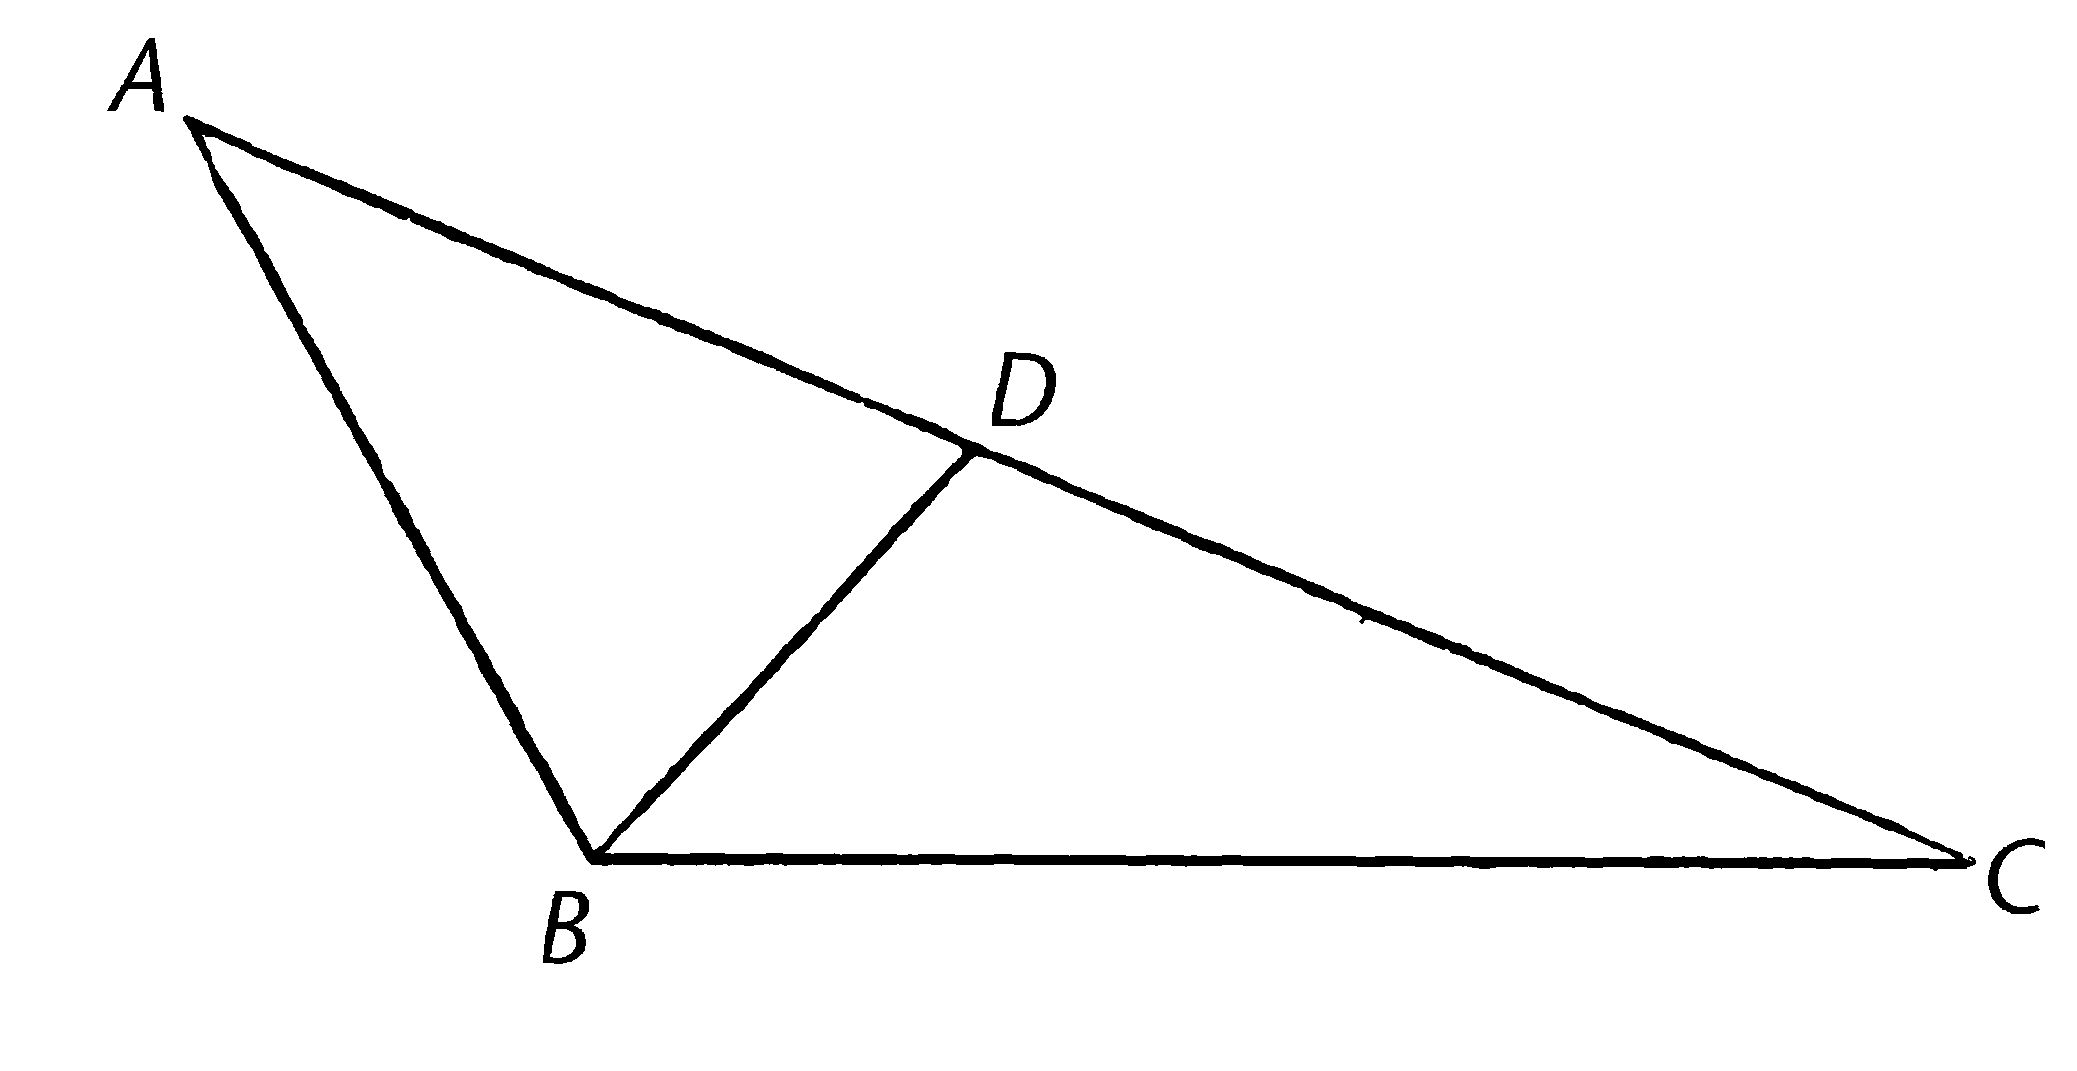
\includegraphics[width=0.4\linewidth]{./image/img485}

设ABC是边AC比边AB长的三角形;我说角ABC比角BCA大。

因为AC比AB长,作AD使等于AB【I.3】,且连接BD。

那么,因为角ADB是三角形BCD的外角,它比内对角DCB大。【I.16】

但是角ADB等于角ABD,因为边AB等于边AD;所以角ABD大于角ACB;角ABC更大于角ACB。

综上所述\ldots{}

Q.E.D.

\hypertarget{ux547dux9898ux5341ux4e5d}{%
\section{命题十九}\label{ux547dux9898ux5341ux4e5d}}

\textbf{在任意三角形中,大角对长边。}

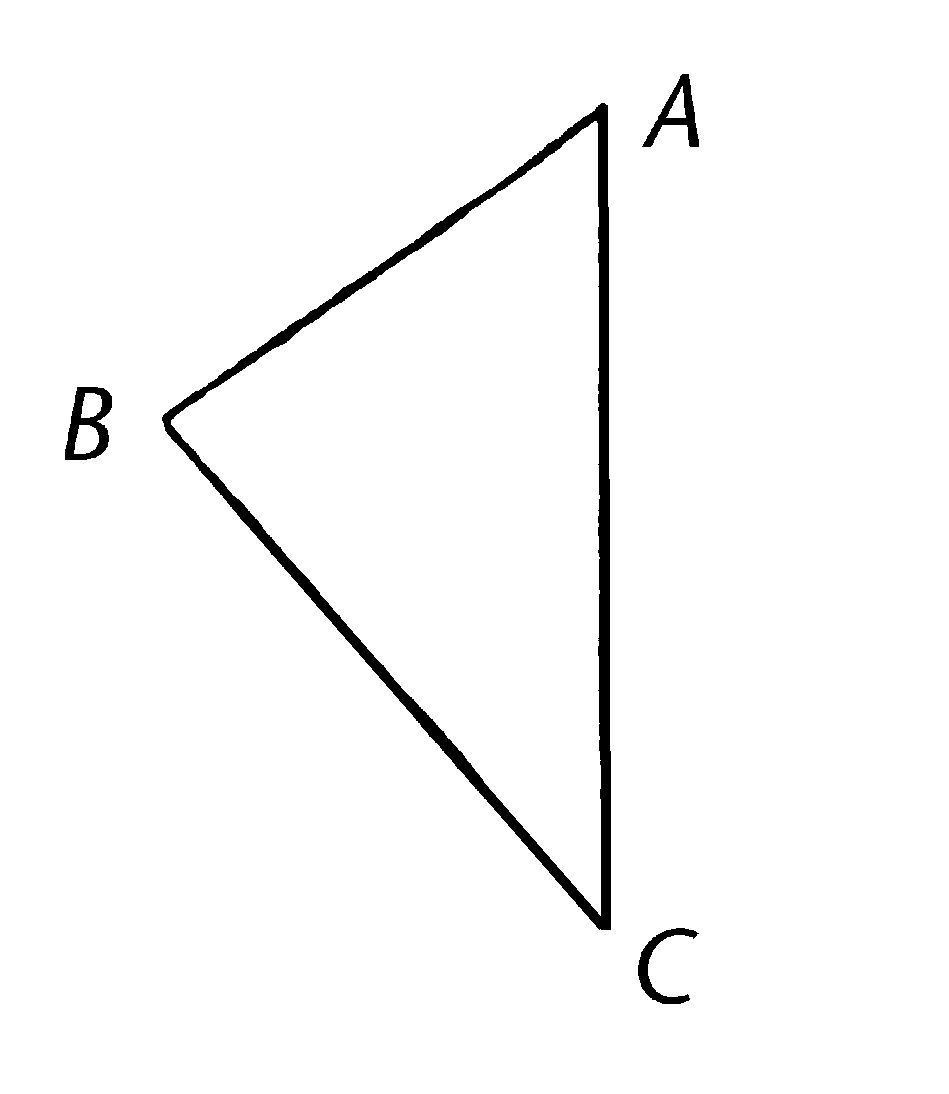
\includegraphics[width=0.3\linewidth]{./image/img487}

设ABC是角ABC比角BCA大的三角形;我说边AC比边AB长。

如果不是的话,AC或等于或小于AB。

现在AC并不等于AB;因为那样的话角ABC应该等于角ACB;【I.5】但是并不是,所以AC并不等于AB。

AC也并不小于AB,因为因为那样的话角ABC应该小于角ACB;【I.5】但是并不是,所以AC并不小于AB。

因为已证明它们也并不相等。

所以AC大于AB。

综上所述\ldots{}

Q.E.D.

问题示例:

\begin{itemize}
\tightlist
\item
  这是前一个命题的逆命题。逆命题需要被证明么?逆命题有时是错的么?
\item
  这个证明用到了归谬,他有辨别出所有的其它可能性么?
\item
  你是否能用I.18和I.5做一个直接的证明?归谬是更简洁么?在逻辑的作用力上,直接证明和归谬有什么不同么?在说服力上呢?
\end{itemize}

\hypertarget{ux547dux9898ux4e8cux5341}{%
\section{命题二十}\label{ux547dux9898ux4e8cux5341}}

\textbf{在任意三角形中,以任意方式取任意两边,其两边之和大于第三边。}

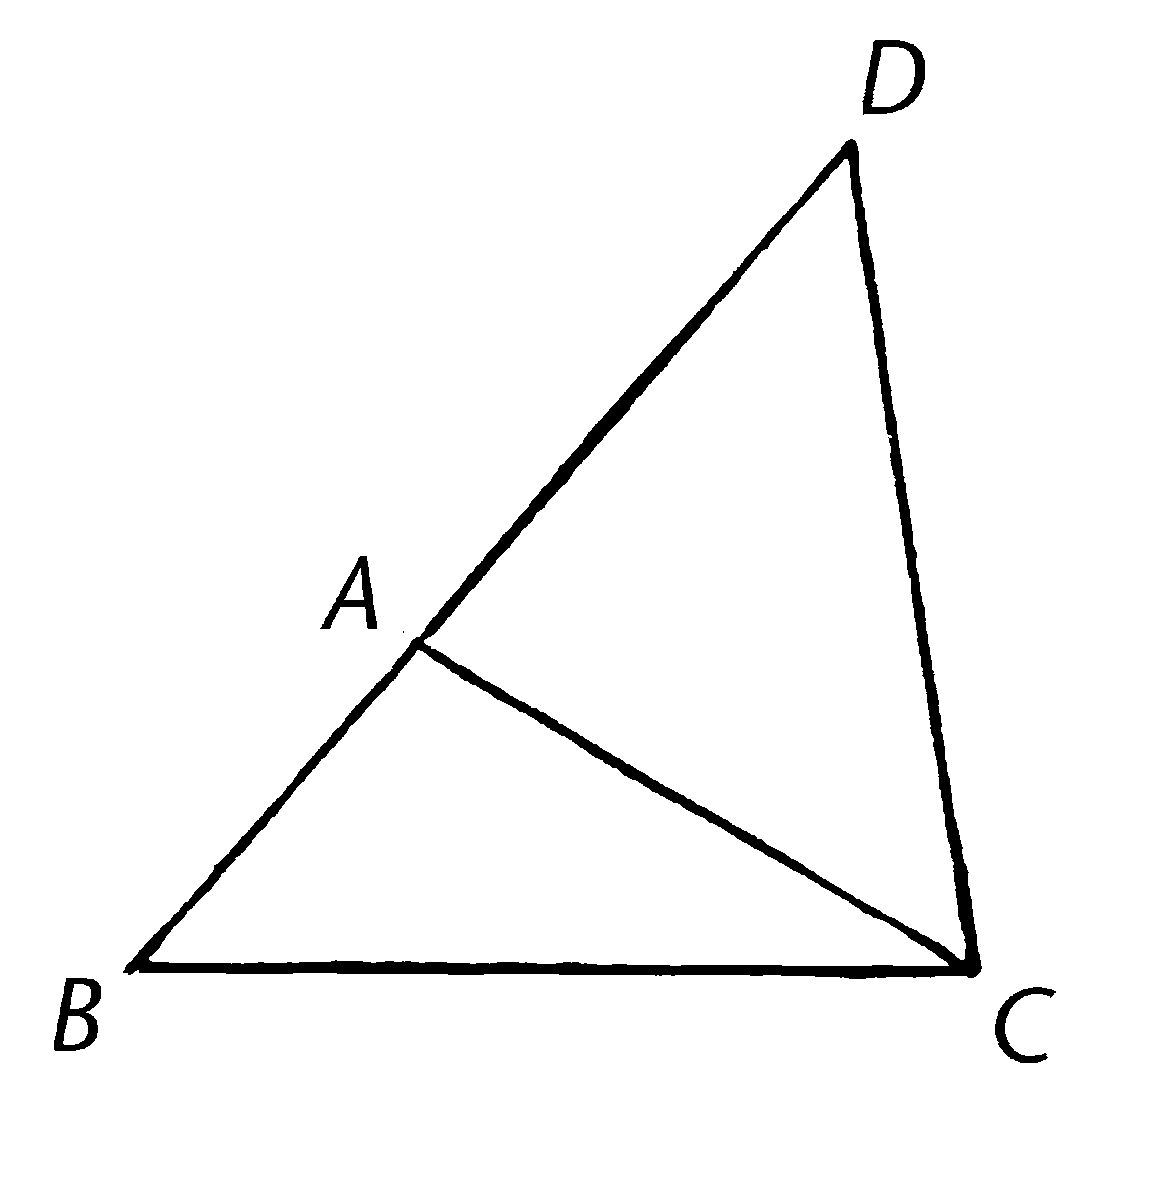
\includegraphics[width=0.3\linewidth]{./image/img489}

设ABC为三角形;我说在三角形ABC中,以任意方式取任意两边,其两边之和大于第三边,即BA,AC大于BC,AB,BC大于AC,BC,CA大于AB。

延长BA至点D,并使DA等于CA,且连接DC。

那么,因为DA等于AC,角ADC也等于角ACD;【I.5】所以角BCD大于角ADC。【公理5】

又因为DCB是角BCD比角BDC大的三角形,且大角对长边,【I.19】,所以DB比BC长。

但是DA等于AC; 所以BA,AC长于BC。

类似地,我们可以证明AB,BC长于CA,且BC,CA长于AB。

综上所述\ldots{}

Q.E.D.

【宣棋注:原文是在任意三角形中,以任意方式取任意两边,其两边之和大于``余边'' ------ remaining side。翻译成第三边是为了更接近平时使用的习惯。】

问题示例:

\begin{itemize}
\tightlist
\item
  Proclus(普罗克鲁斯), 一个五世纪在亚历山大港的评论员,说伊壁鸠鲁学派的人喜欢通过驴都知道这个真理的说法嘲笑这个命题,因为没有驴会通过三角形的两边而不是直线去接近食物。确实如此,这似乎仅仅是通过看或者想象三角形,就是直观明显的。但是那是证明么?Proclus说仅仅察觉某事物的真相是不够的:要形成知识,我们必须知道它为什么是真的。你同意么?
\item
  我们是不是回到了关于图像和通过言语论证的问题?在这个命题中,图像里显而易见的内容被证明为真。(至少如果你想要最短的时间去午餐的话)但是,会不会有些看起来明显的图像结果变地迷惑人或完全的错误?你曾见过埃舍尔的绘画么?
\end{itemize}

【宣棋注:举例天才画家M.C.Escher的作品《升与降》】

\hypertarget{ux547dux9898ux4e8cux5341ux4e00}{%
\section{命题二十一}\label{ux547dux9898ux4e8cux5341ux4e00}}

\textbf{如果在三角形的一边,从其端点,构建两条直线使相交于三角形内,这两条直线比三角形剩余的两边短,但夹角更大。}

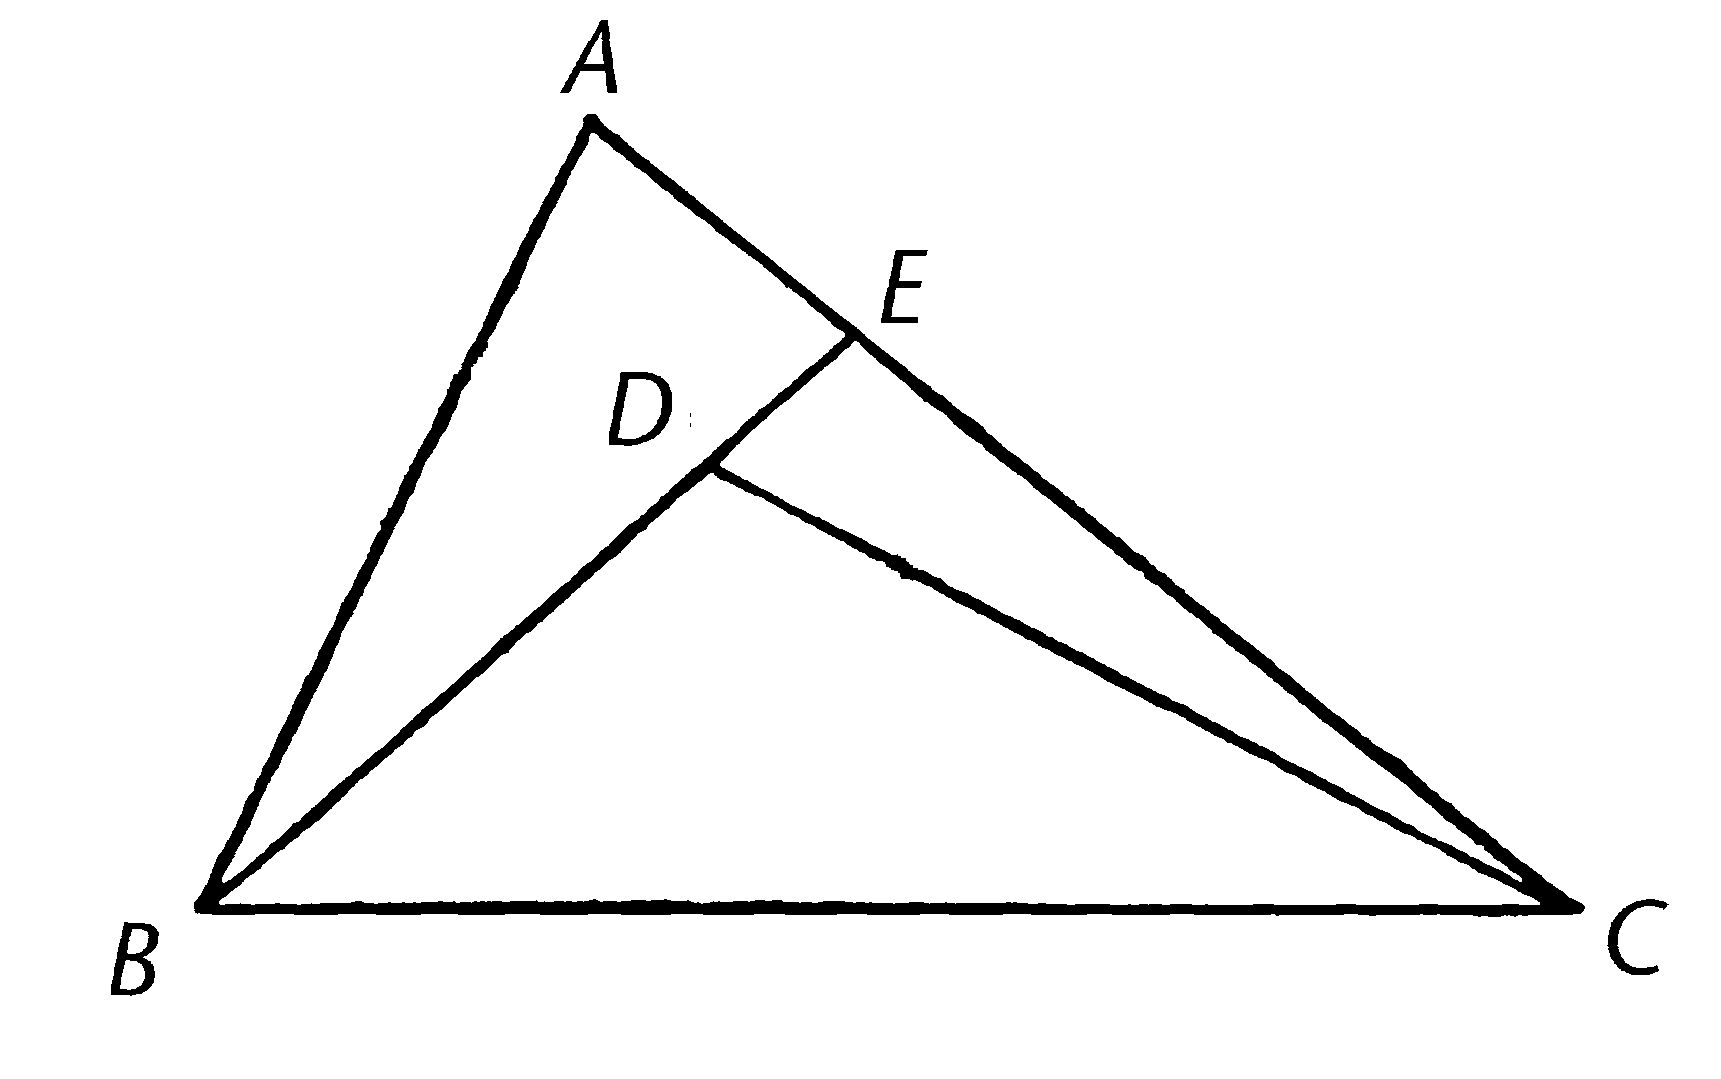
\includegraphics[width=0.3\linewidth]{./image/img491}

在三角形ABC的其中一边BC上, 由其端点B,C构建两条直线BD,DC,并使其在三角形内相交。

我说BD,DC比剩余两边BA,AC短,但是其夹角BDC比角BAC大。

延长BD到E。

那么,因为在任意三角形中,任意两边之和大于第三边,【I.20】所以,在三角形ABE中,两边AB,AE大于BE。

各自添加EC,那么BA,AC大于BE,EC。

再一次,因为在三角形CED中,两边CE,ED大于CD, 各自添加DB,那么CE,EB大于CD,DB。

但是已证明BA,AC要远大于BD,DC。

再一次,在任意三角形中,如果延长其中一边,那么外角大于内对角,【I.16】那么,在三角形CDE中,外角BDC大于角CED。

此外,同理可得,在三角形ABE中,外角CEB大于角BAC。

但是已证明角BDC大于角CEB;所以角BDC远大于角BAC。

综上所述\ldots\ldots{}

Q.E.D.

\hypertarget{ux547dux9898ux4e8cux5341ux4e8c}{%
\section{命题二十二}\label{ux547dux9898ux4e8cux5341ux4e8c}}

\textbf{由分别等于三条已知线段的线段构建一个三角形:那么必须满足任取其中两条线段,其和大于第三边。}

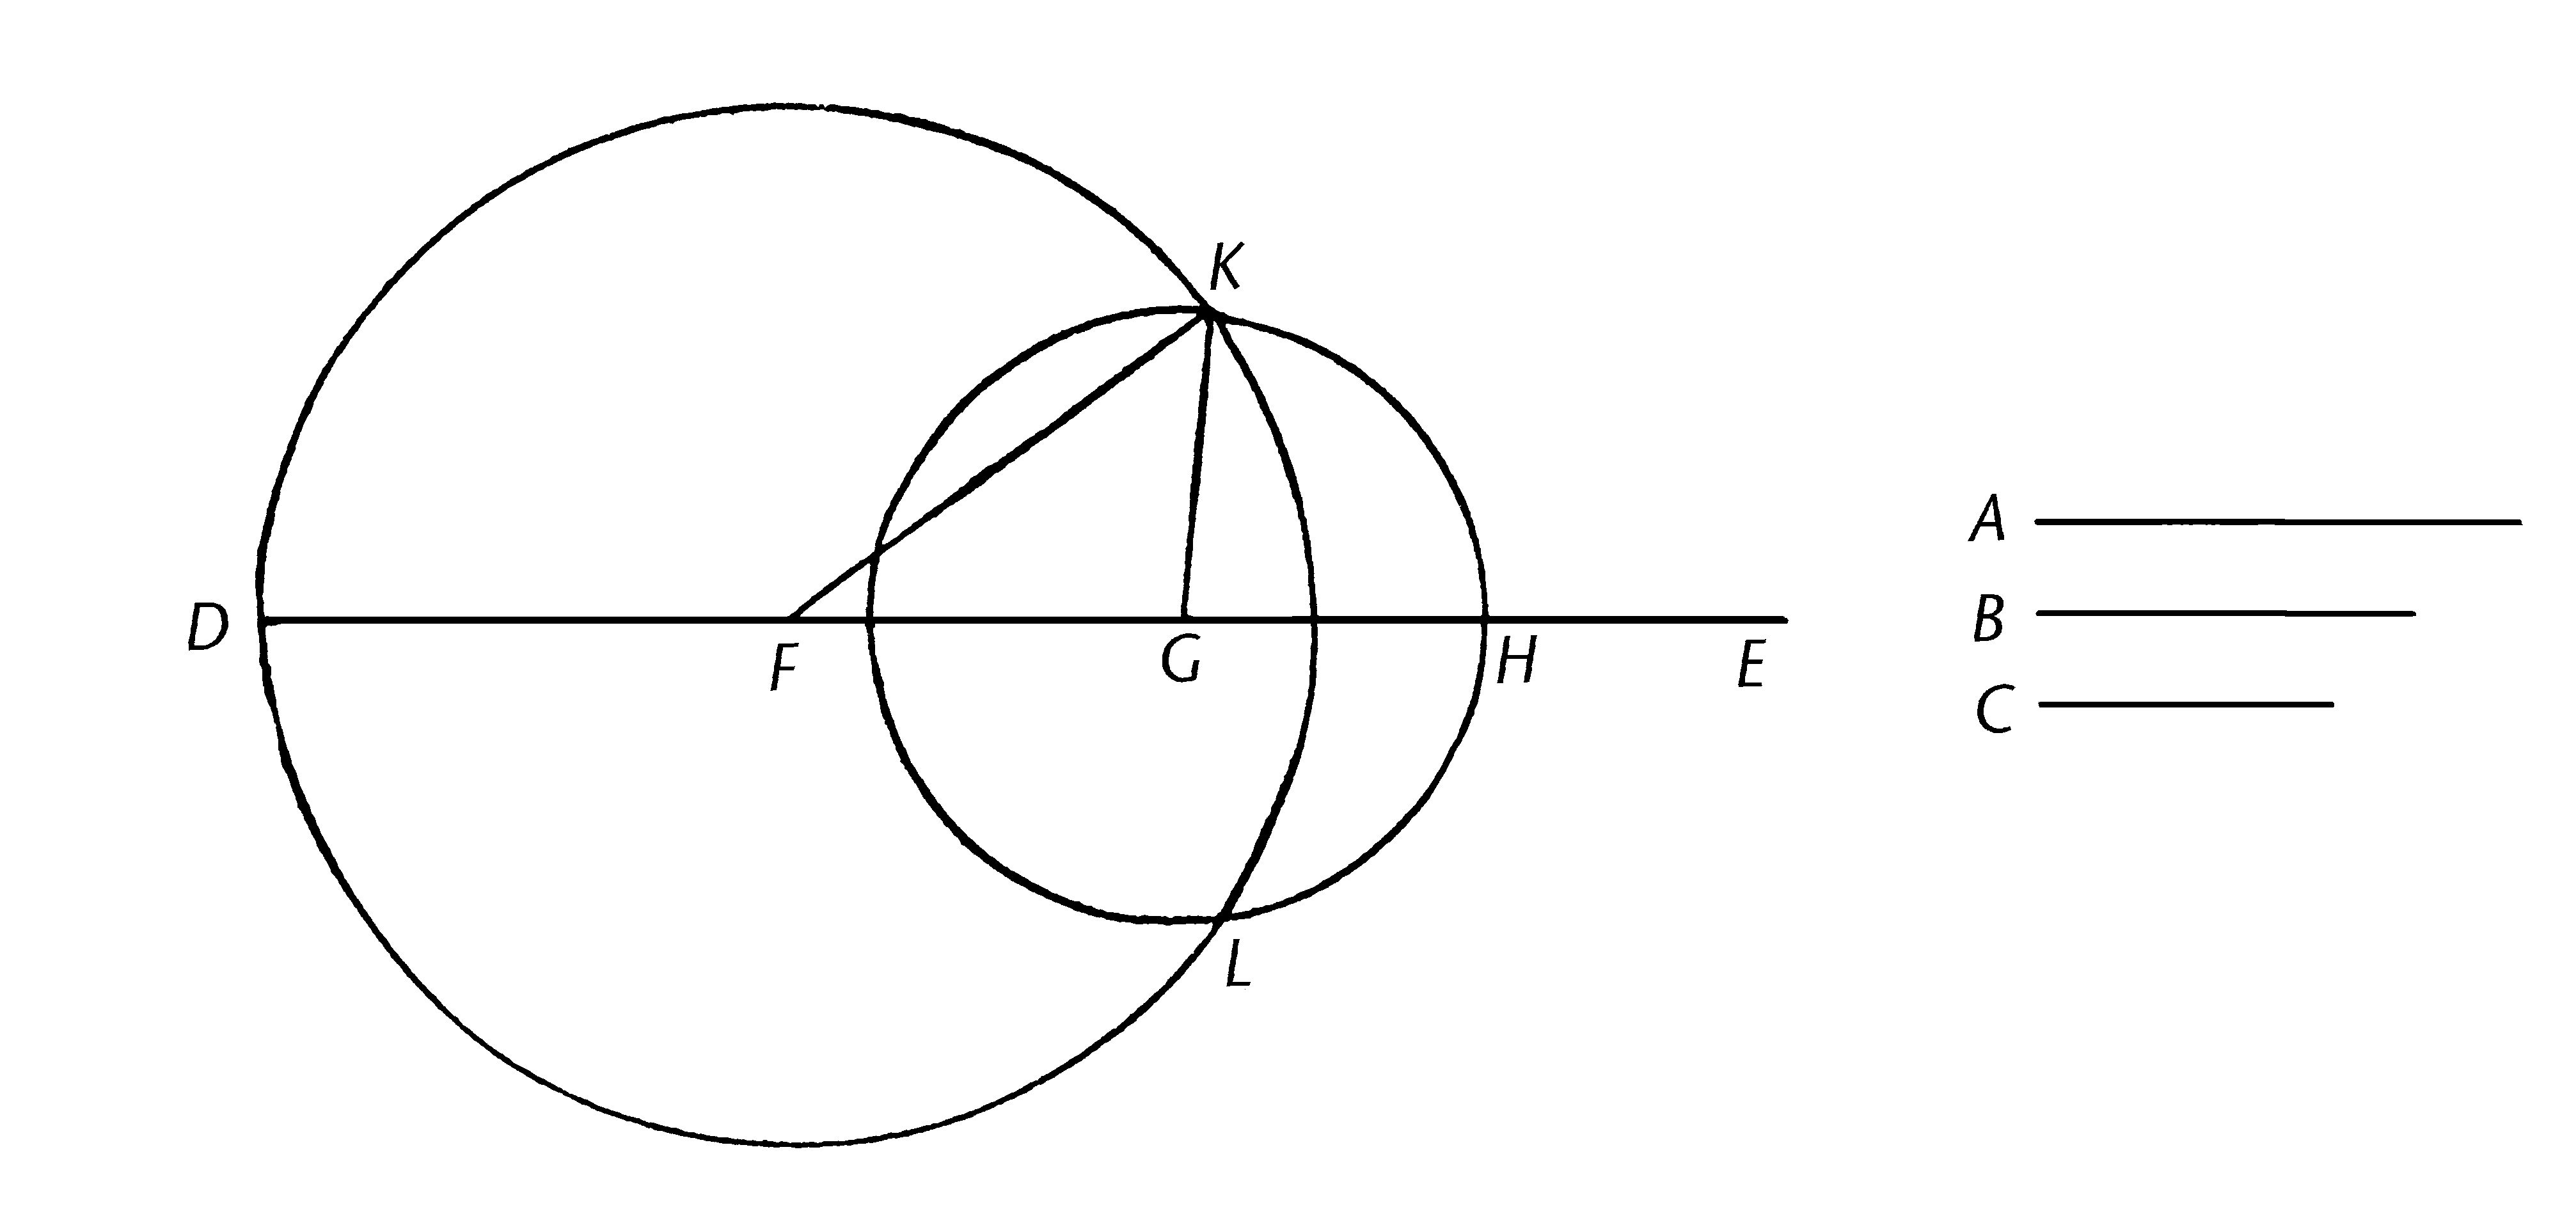
\includegraphics[width=0.5\linewidth]{./image/img493}

给定三条直线A,B,C,且任取其中两条之和大于第三条,即A,B大于C,A,C大于B,且BC大于A;那么需要以与A,B,C相等的直线构建一个三角形。

设直线DE,一端为D但是在E方向无限长,且使DE与A相等,FG与B相等,GH与C相等。【I.3】

以F为圆心,FD为距离,画圆DKL;再一次,以G为圆心,GH为距离,画圆KLH,且连接KF,KG;我说三角形KFG使以与A,B,C相等的三条直线构建的。

因为,点F是圆DKL的圆心,FD等于FK。

但是FD等于A;所以KF也等于A。

再一次,因为点G是圆LKH的圆心,GH等于GK。

但是GH等于C;所以KG也等于C。

且FG等于B;所以三条直线KF,FG,GL等于三条直线A,B,C。

所以,三角形KFG由三条等于给定直线A,B,C的EF,FG,GK构建而成。

Q.E.F.

问题示例:

\begin{itemize}
\tightlist
\item
  为什么任意两条直线之和必须大于第三边?当然的,如果这不是真的,在命题20中,我们已经可以展示这样不能构建三角形。这里有更多深意么?我们如何知道两个圆相交会形成我们所需要的三角形?
\item
  通过这个命题,你有享受通过线、角以及三角形构建的这种方式么?你是否有留意不同命题的组合?你能草绘一个流程图或者一个模型么,关于卷一中的体系是如何构建的?
\end{itemize}

\hypertarget{ux547dux9898ux4e8cux5341ux4e09}{%
\section{命题二十三}\label{ux547dux9898ux4e8cux5341ux4e09}}

\textbf{从给定的直线上一点,构建一个直线角,使等于给定的直线角。}

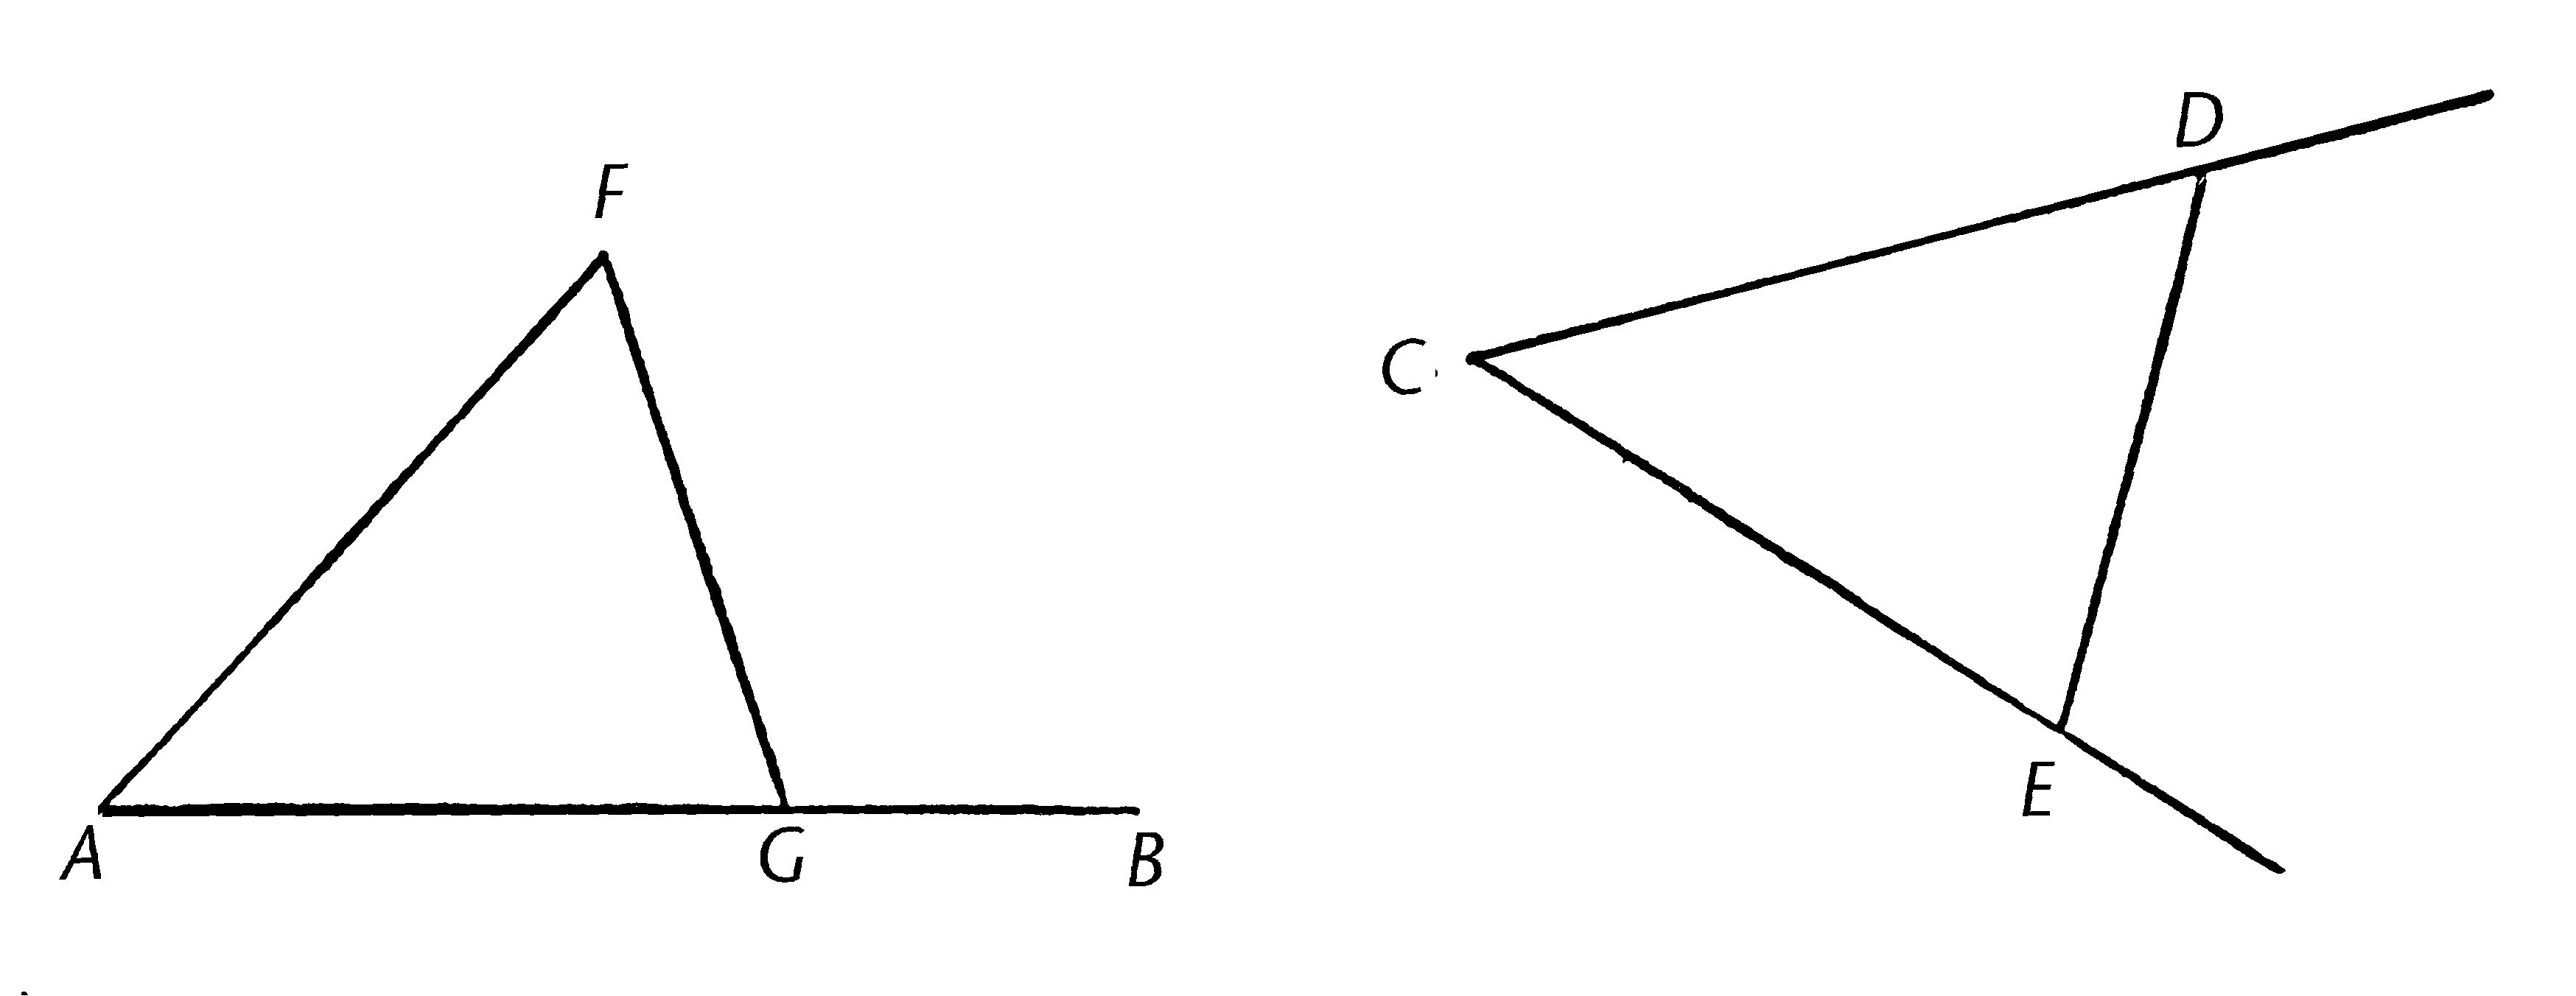
\includegraphics[width=0.5\linewidth]{./image/img496}

给定直线AB, A为其上一点,且角DCE是给定的直线角;那么需要在给定直线AB及点A上构建一个直线角,与给定的直线角DCE相等。

在直线CD,CE上分别随意取点D,E;连接DE,并且由三条等于CD,DE,CE的直线构建三角形AFG,使得CD等于AF, CE等于AG,且DE等于FG。【I.22】

接下来,因为两边DC,CE分别等于两边FA,AG;且底DE等于底FG,角DCE等于角FAG。【I.8】

所以在给定直线AB的点A上,构建了与给定直线角DCE相等的角FAG。

Q.E.F.

问题示例:

\begin{itemize}
\tightlist
\item
  有趣的是,为了重新画一个角,他构建了一个含有该角的三角形。角本身不是一个事物,只是三角形的一部分么?那么什么是角呢?(当然角已经在定义8-12定义过了)它是一个脱离**(三角形)的事物,两条线之间的倾斜度?还是说问题不在角上,更重要的是他用来构建角的工具?当他探索三角形的性质时,他的工具才显现出来。
\item
  在I.4中,我们拾起三角形并且放置它,这是可以的,为什么在这儿我们不可以这样做呢?(我们注意到这个可能的捷径也能够用在之前的命题里。)我们有察觉到调用这个技巧的勉强么?我们能感受到欧几里得对此的不适么?
\item
  I.23依赖于I.22:用三条给定(有合适长度关系的)直线构建三角形。但是这里有一个I..22没有展现的条件:我们必须将这个角(以及包含这个角的三角形)放在给定直线的给定点上。所以我们能否用I.22中同样的方法构建呢?圆会在``线等于线''的论证中落于我们所寻的角附近合适的位置么?你如何测量线并且以不同的方式画圆呢?
\end{itemize}

\hypertarget{ux547dux9898ux4e8cux5341ux56db}{%
\section{命题二十四}\label{ux547dux9898ux4e8cux5341ux56db}}

\textbf{如果两个三角形的两边分别对应相等,但是它们的夹角,其中一个比另一个大,那么相应的底边也长于另一个底边。}

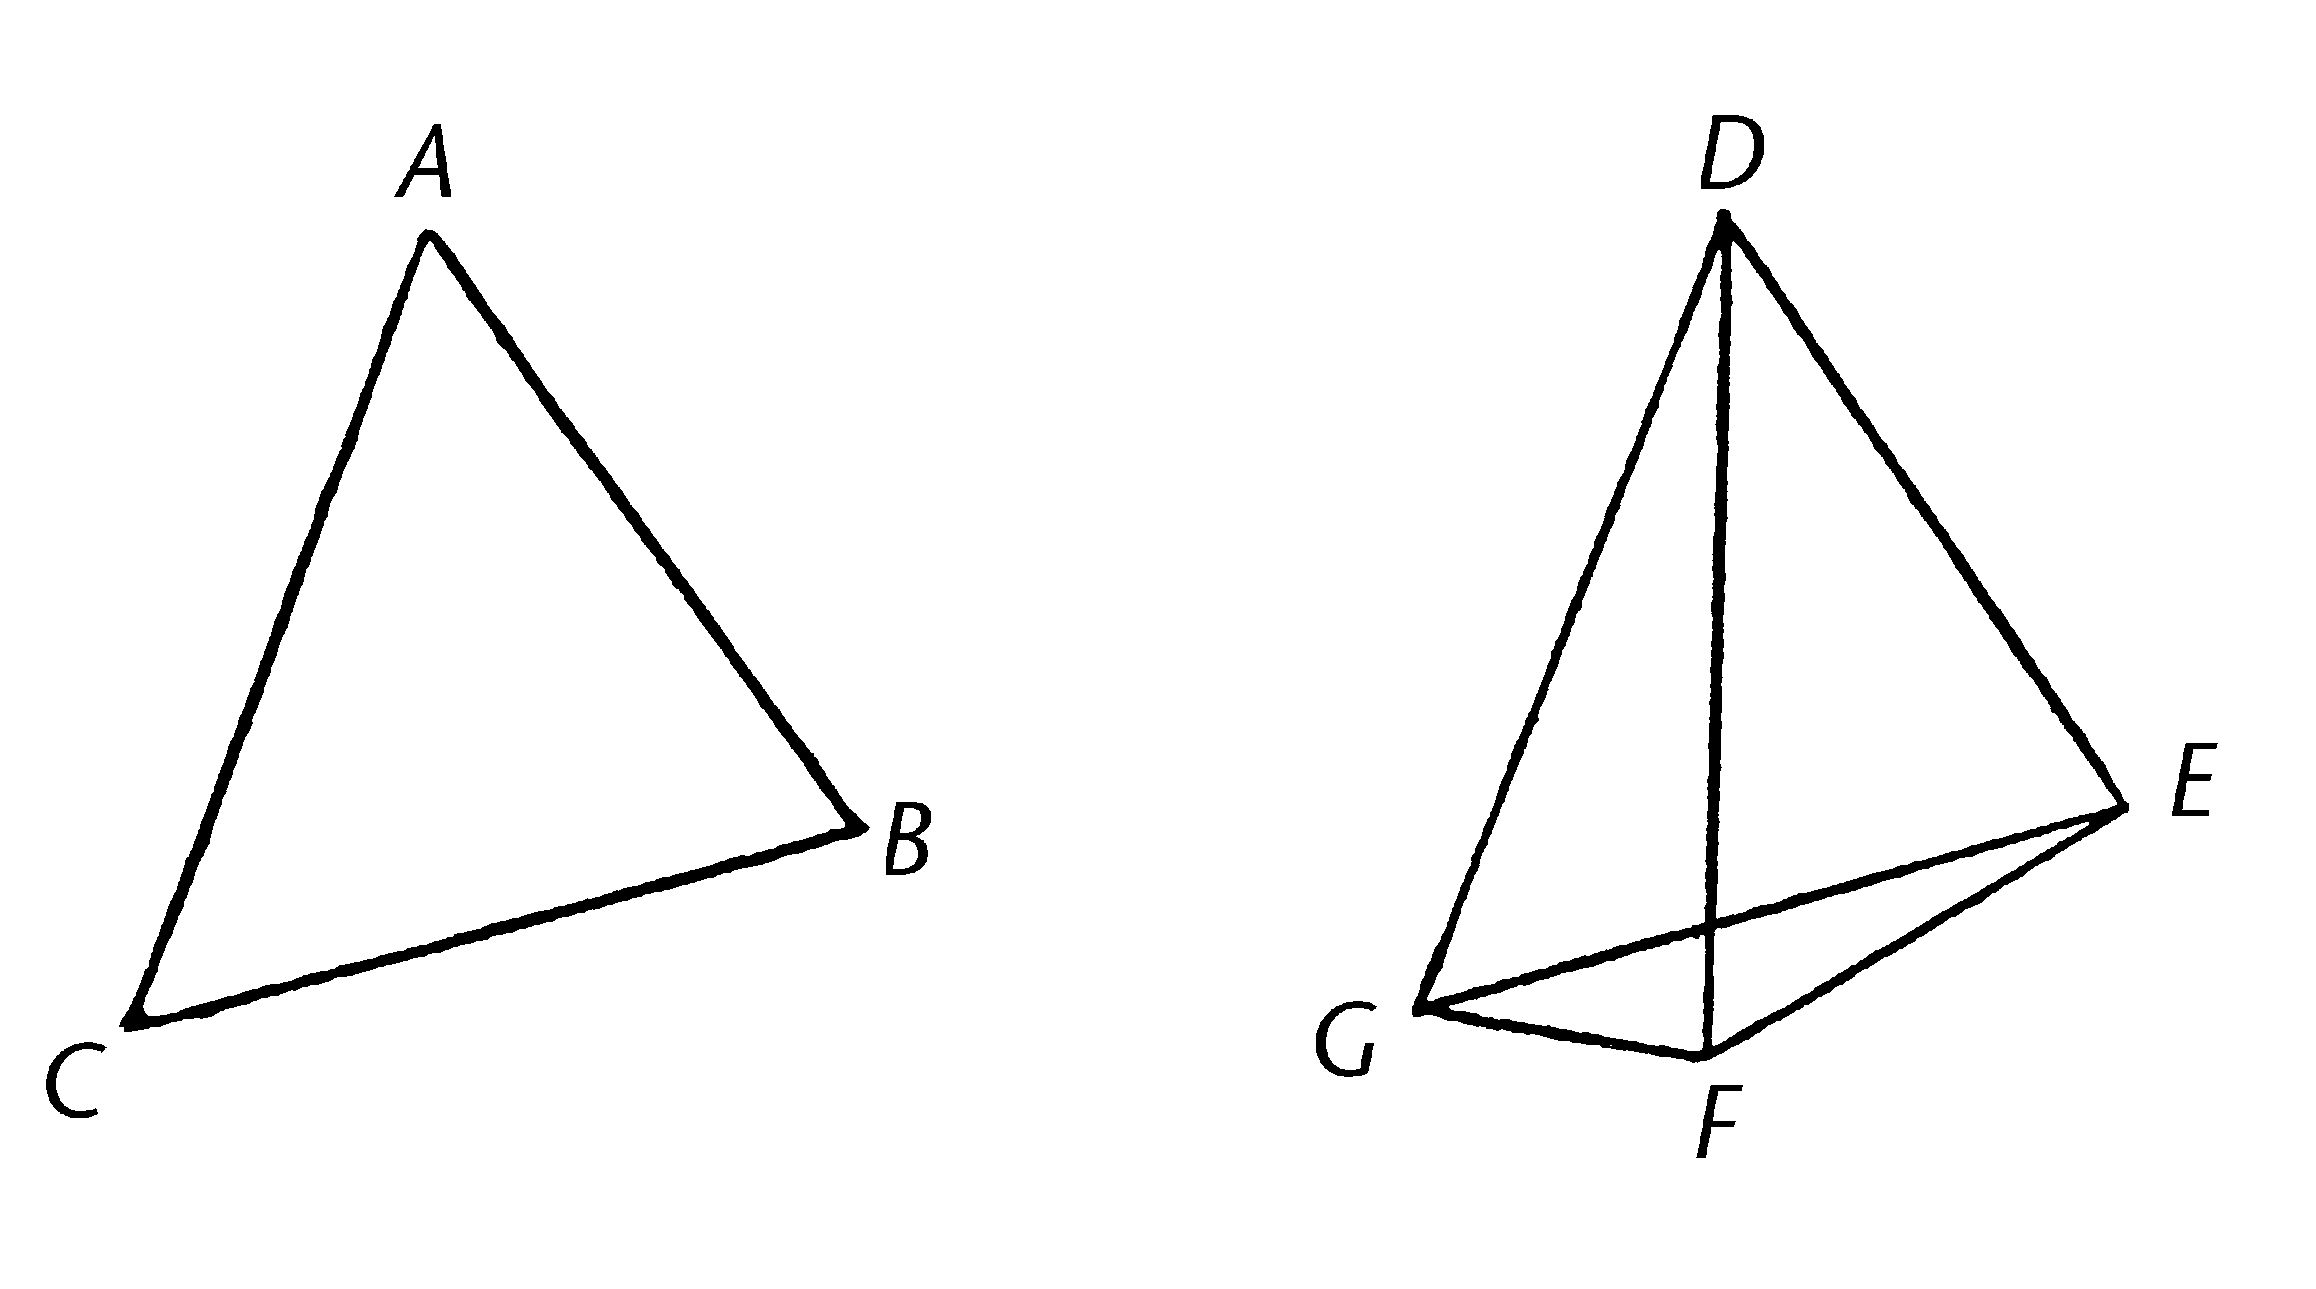
\includegraphics[width=0.5\linewidth]{./image/img499}

ABC,DEF是两个两边AB,AC与DE,DF分别相等的三角形,即AB等于DE,AC等于DF,使A处的角比D处的角大;我说底BC也比底EF长。

因为角BAC大于角EDF,在直线DE的点D上,构建角EDG等于角BAC;【I.23】作DG等于直线AC或DF,且连接EG,FG。

那么,因为AB等于DE, 且AC等于DG,两边BA,AC分别等于两边ED,DG。【I.4】

再一次,因为DF等于DG,角DGF等于角DFG;【I.5】所以叫DFG大于角EGF。

所以角EFG远大于角EGF。

又因为EFG是角EFG比角EGF大的三角形,大角对长边,【I.19】边EG也长于EF。

但是EG等于BC。所以BD也长于EF。

综上所述\ldots\ldots{}

Q.E.D.

问题示例:

\begin{itemize}
\tightlist
\item
  之前,我们在命题7中讨论是否图像仅代表一种示例但存有其它可能性,这里的情况与之相似么?你是否有留意到命题7中只有一种假设,而这个命题的设置里包含了其它情况?
\item
  如果点G落在其它地方,比如说线EF之下,或者EF的延长线上,那么证明会发生怎样的变化?欧几里得有给予我们最难的示例,将其它简单变化过较容易的证明视为没有必要详细说明么?你是否能草绘证明其它可能的情况,来确认此命题的真实性?
\end{itemize}

\hypertarget{ux547dux9898ux4e8cux5341ux4e94}{%
\section{命题二十五}\label{ux547dux9898ux4e8cux5341ux4e94}}

\textbf{如果两个三角形的两边各自对应相等,但是其中一个底边更长,那么它们的夹角更大。}

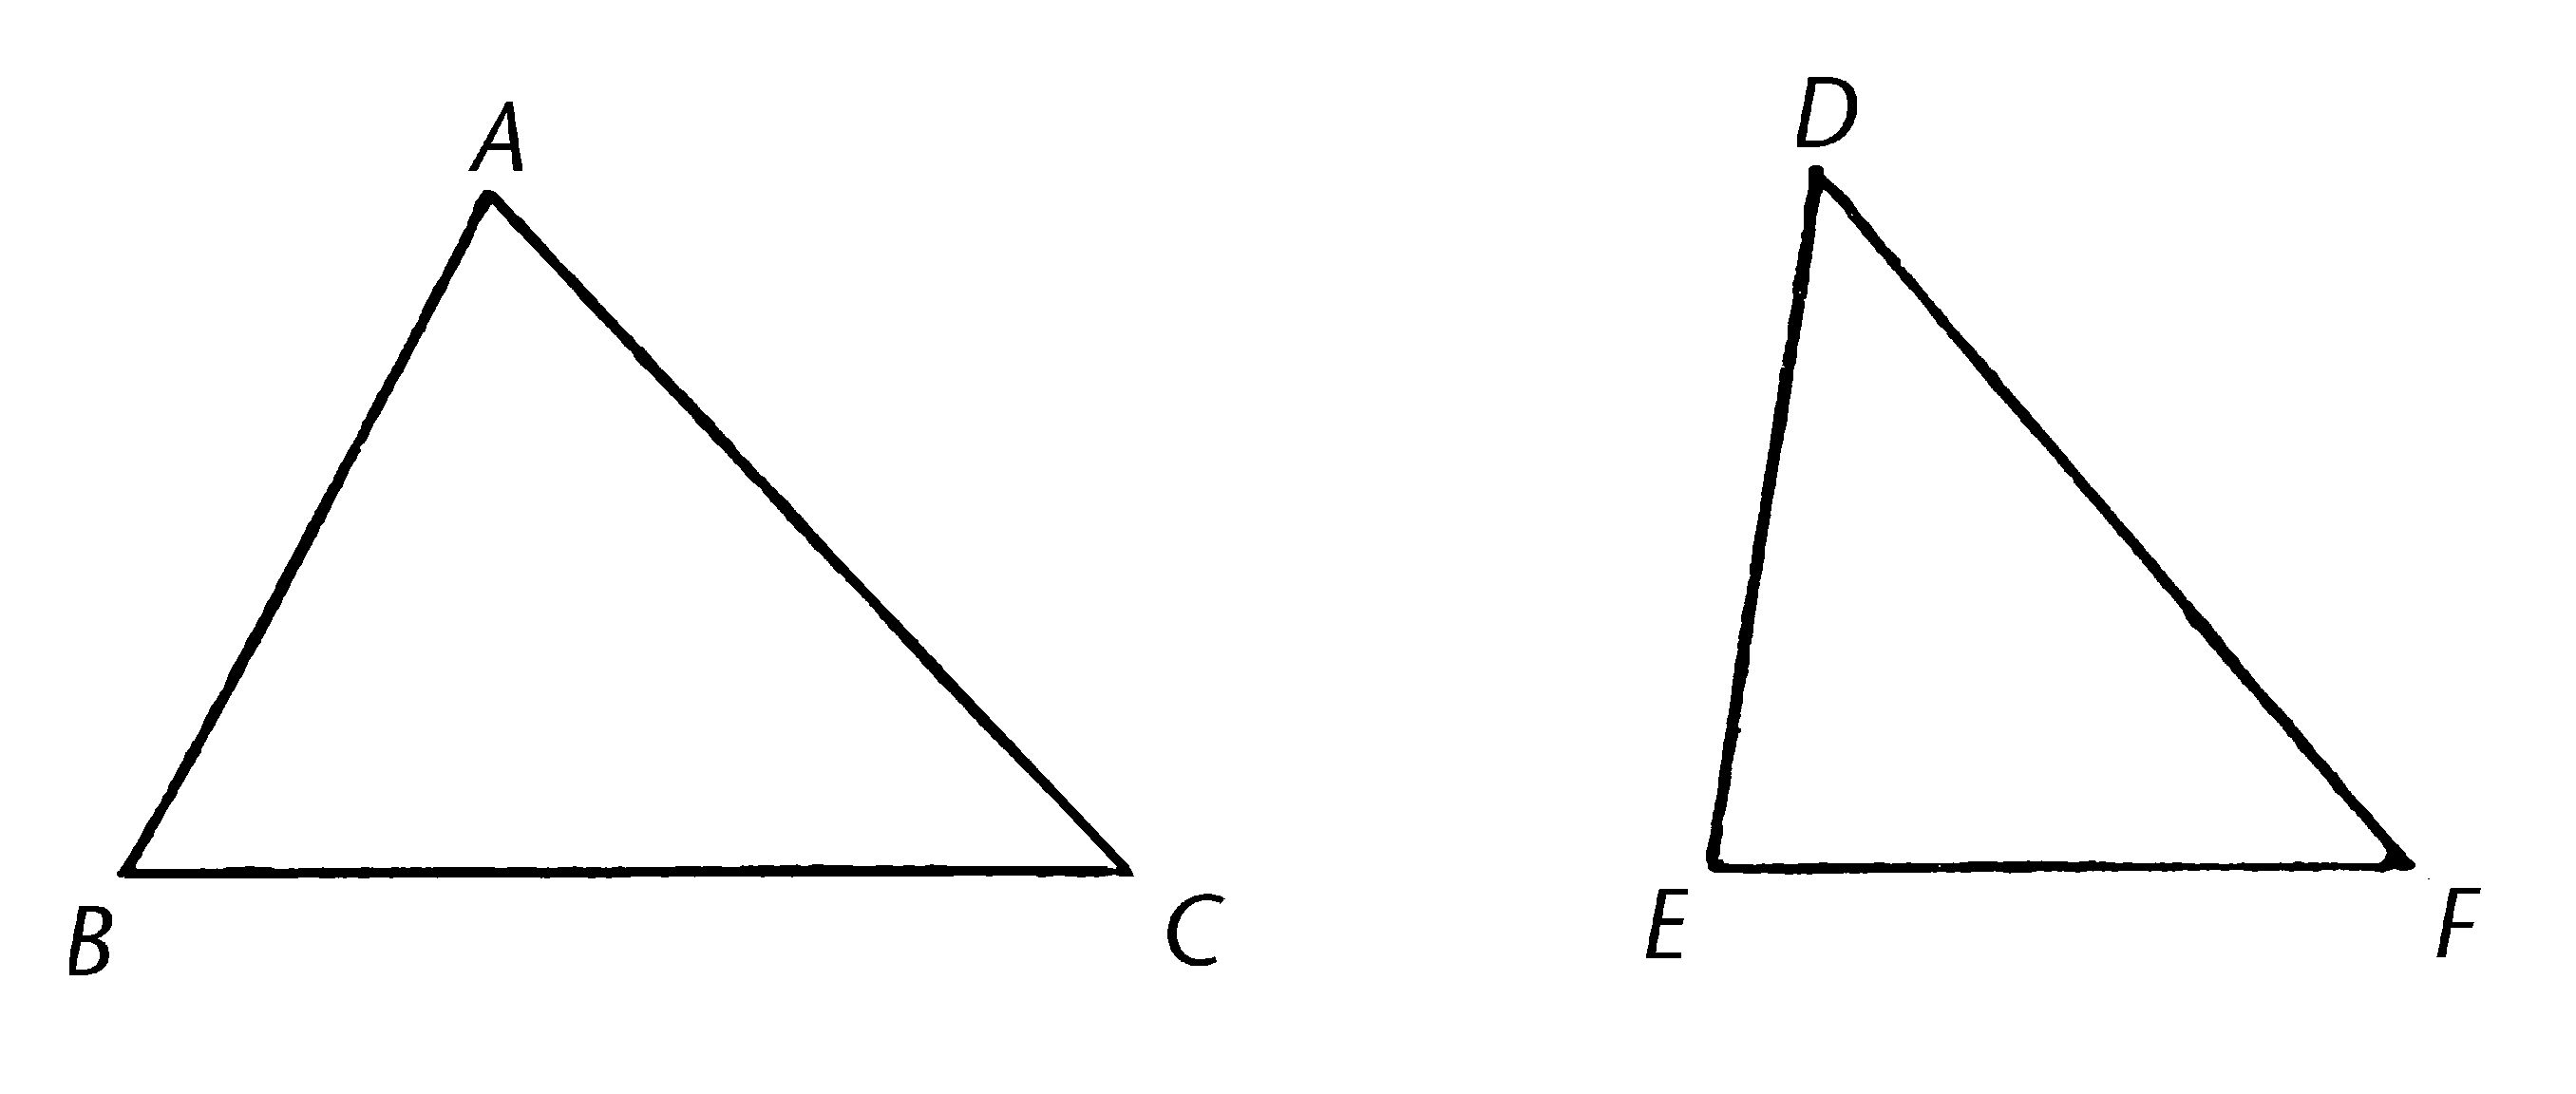
\includegraphics[width=0.5\linewidth]{./image/img502}

ABC,DEF是两个两边AB,AC与DE,DF分别相等的三角形,即AB等于DE,AC等于DF,底BC比底EF长; 我说角BAC也比角EDF大。

因为,如果不是的话,或者相等,或者小于。

现在角BAC不等于角EDF; 否则底BC也应等于底EF【I.4】,但是并没有;所以角BAC不等于角EDF。

再一次,角BAC也不小于角EDF;否则底BC也应小于底EF【I.24】,但是并没有;所以角BAC不小于角EDF。

但是已证明它们也不相等;所以角BAC大于角EDF。

综上所述\ldots\ldots{}

Q.E.D.

\hypertarget{ux547dux9898ux4e8cux5341ux516d}{%
\section{命题二十六}\label{ux547dux9898ux4e8cux5341ux516d}}

\textbf{如果两个三角形中的两角各自对应相等,并且其中一边等于另一边,即或者等角的临边,或者等角的对边,那么它们剩余的边和角也都对应相等。}

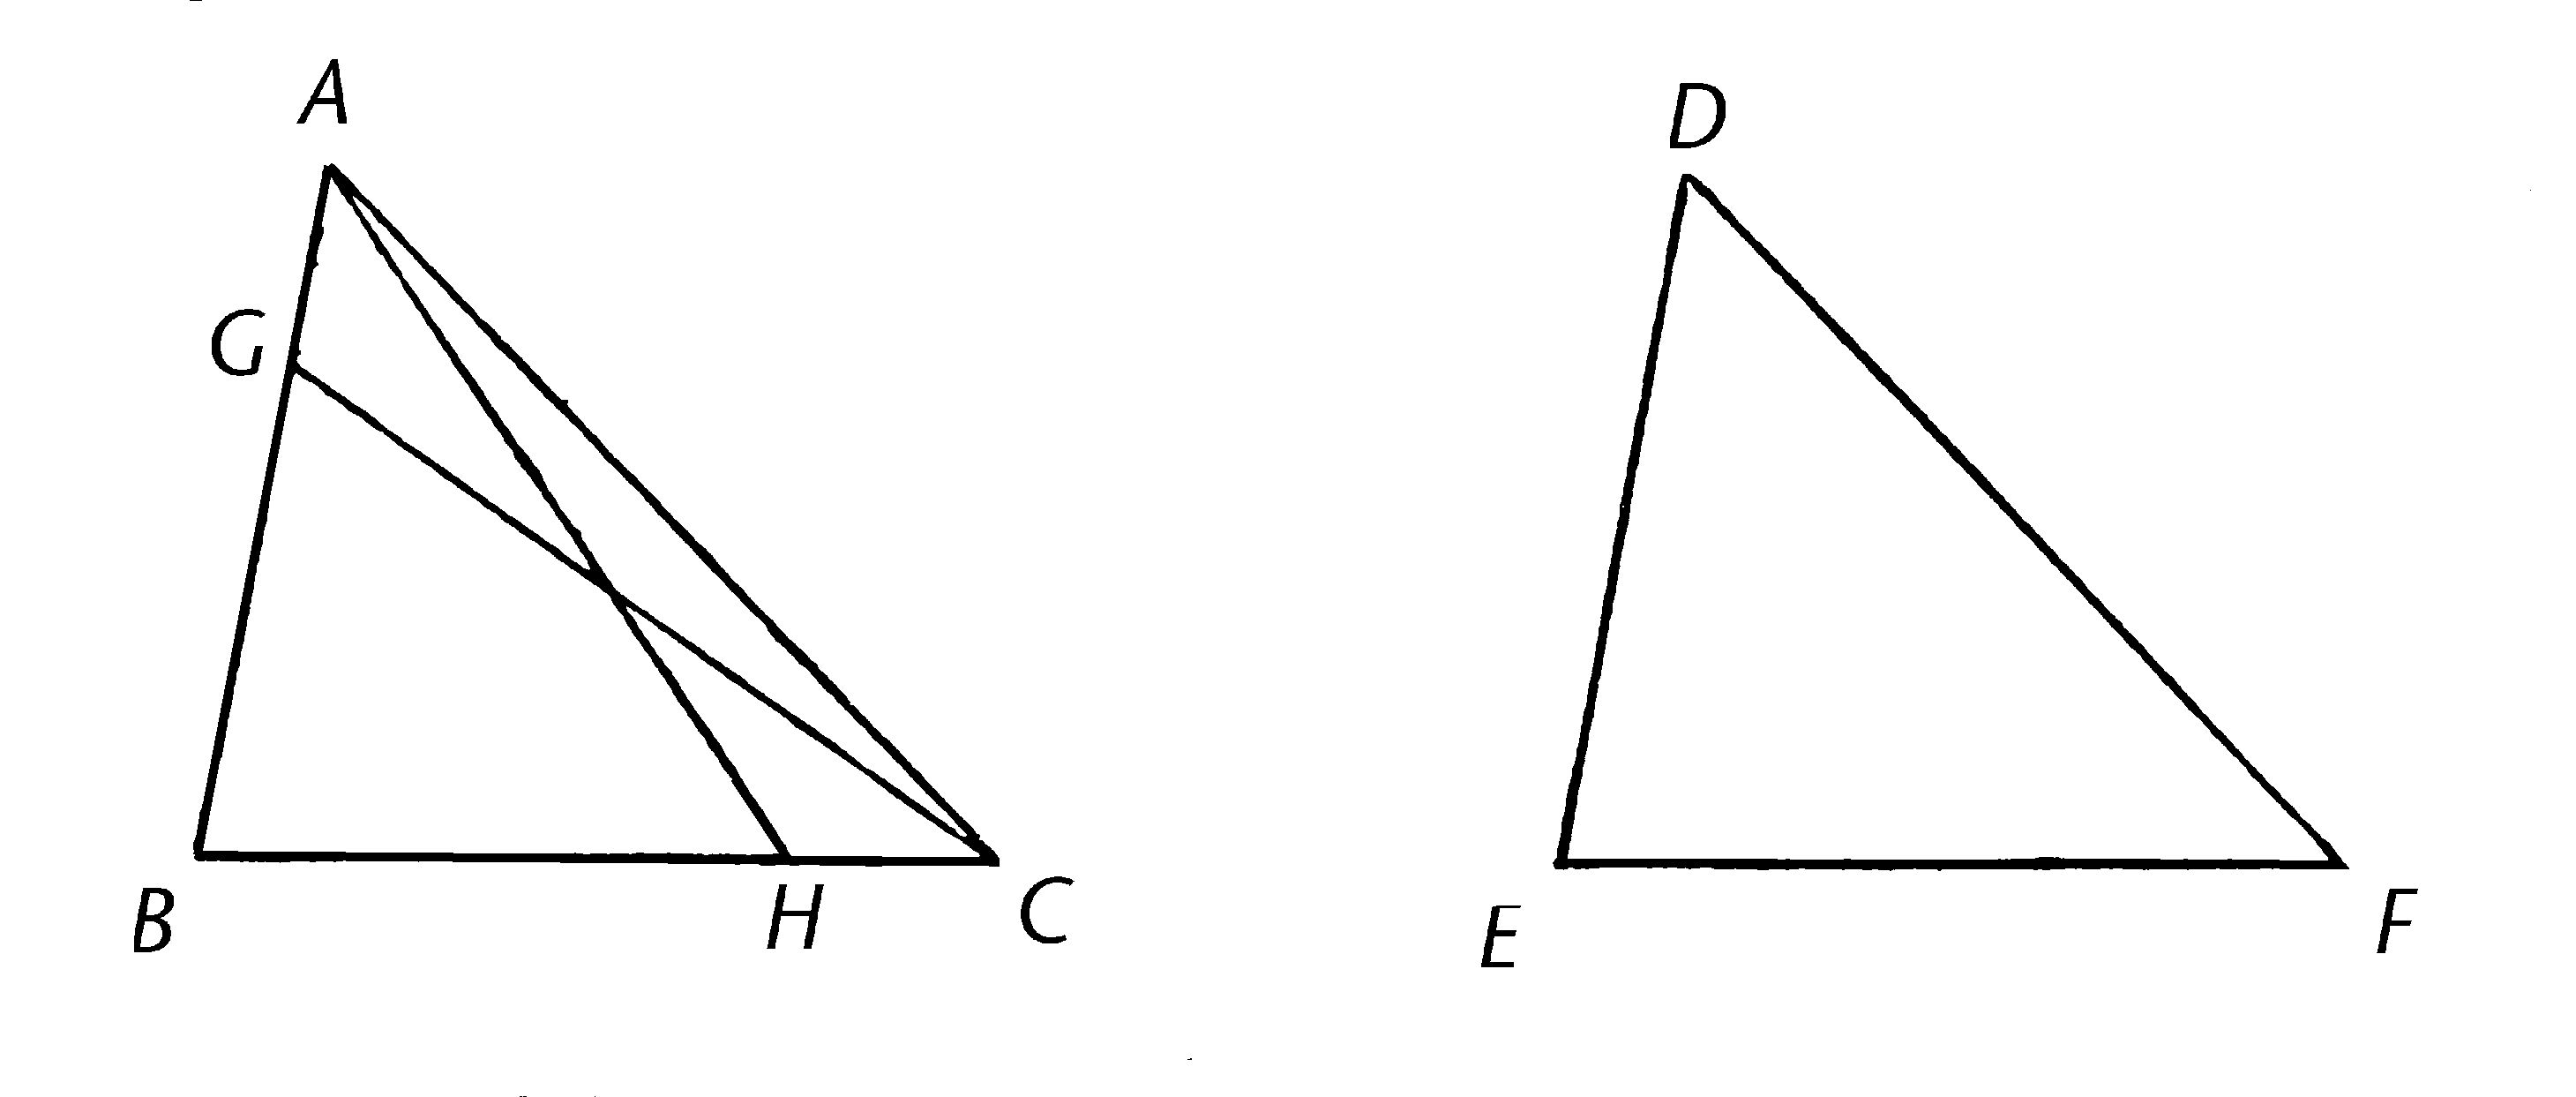
\includegraphics[width=0.5\linewidth]{./image/img504}

ABC,DEF是两个三角形,其中两角ABC,BCA与两角DEF,EFD互等,即角ABC与角DEF,角BCA与角EFD;使它们其中一边也互等,首先使两等角所夹的边相等,即BC与EF;我说它们剩余的边也互等,即AB与DE,AC与DF,且剩余的角互等,即角BAC与角EDF。

因为,如果AB不等于DE,它们其中之一会更长。

使AB更长,并使得BG等于DE;且连接GC。

那么,因为BG等于DE,BC等于EF,两边GB,BC分别等于两边DE,EF;且角GBC等于角DEF;所以底边GC等于底边DF,且三角形GBC等于三角形DEF,且剩余的角也互等,即等边所对的角【I.4】;那么角GCB等于角DFE。

但是由假设角DFE等于角BCA;那么角BCG等于角BCA,小的等于大的:这是不可能的。

所以AB不能不等于DE,即AB等于DE。

但是BC也等于EF;所以两边AB,BC与两边DE,EF互等;且角ABC等于角DEF;所以底边AC等于底边EF, 且剩余的角BAC等于剩余的角EDF。【I.4】

再一次,使等角对应的边相等,即AB与DE;我再说剩余的边互等,即AC与DF,BC与EF,剩余的角BAC等于剩余的角EDF。

因为,如果BC不等于EF,那么其中之一会更长。

使BC更长,如果可能的话,并使得BH等于EF;且连接AH。

那么,因为BH等于EF,AB等于DE,两边AB,BH分别等于两边DE,EF;且它们所夹的角互等;所以底边AH等于底边DF,且三角形ABH等于三角形DEF,且剩余的角也互等,即等边所对的角【I.4】;那么角BHA等于角EFD。

但是角EFD等于角BCA;所以在三角形AHC中,外角BHA等于内对角BCA:这是不可能的。【I.16】

所以BC不能不等于EF:即BC等于EF。

但是AB也等于DE;所以两边AB,BC与两边DE,EF互等;且它们所夹的角互等;所以底边AC等于底边DF, 三角形ABC等于三角形DEF,且剩余的角BAC等于剩余的角EDF。【I.4】

综上所述\ldots\ldots{}

Q,E.D.

问题示例:

\begin{itemize}
\tightlist
\item
  现在,我们扩大了对论证全等的工具收藏。我们被给予两组彼此互等的角。我们证明(1)如果两角之间的边也相等,那么剩余的边和角都相等,然后(2)如果两等角之一对应的临边也相等,那么剩余的边和角也相等。这些新关系的简写形式是什么?
\item
  为什么我们不能说,如果我们有两组等角,则所有的角都互等(允许证明几乎由I.4直接导出)?还是说这里会有一个关于我们在其它地方所学事物的错误应用,还是说它只是看起来``显而易见'',但其实我们尚未证明?在这种情况下,为了知道第三个角也相等,什么是我们需要但缺失的?
\item
  为什么欧几里得等了这么久才论证它们的关系?第一部分仅仅调用了I.4,而第二部分仅仅调用了I.16。是因为他在此之前并不需要它们么?在展开这个体系的时候,在这儿是不是存在一种工作的简省?
  我们完成了这本书的很长一部分,为线,角,三角形和它们之间的关系,部分,构建奠定了基础。现在,我们将前行至关于平行和深入理解区域相等性的工作,如果你有之前作了流程图,这是个审视它的绝妙时机。
\end{itemize}

\hypertarget{ux547dux9898ux4e8cux5341ux4e03}{%
\section{命题二十七}\label{ux547dux9898ux4e8cux5341ux4e03}}

\textbf{如果一条直线落在两条直线上并使得内错角互等,那么两条直线平行。}

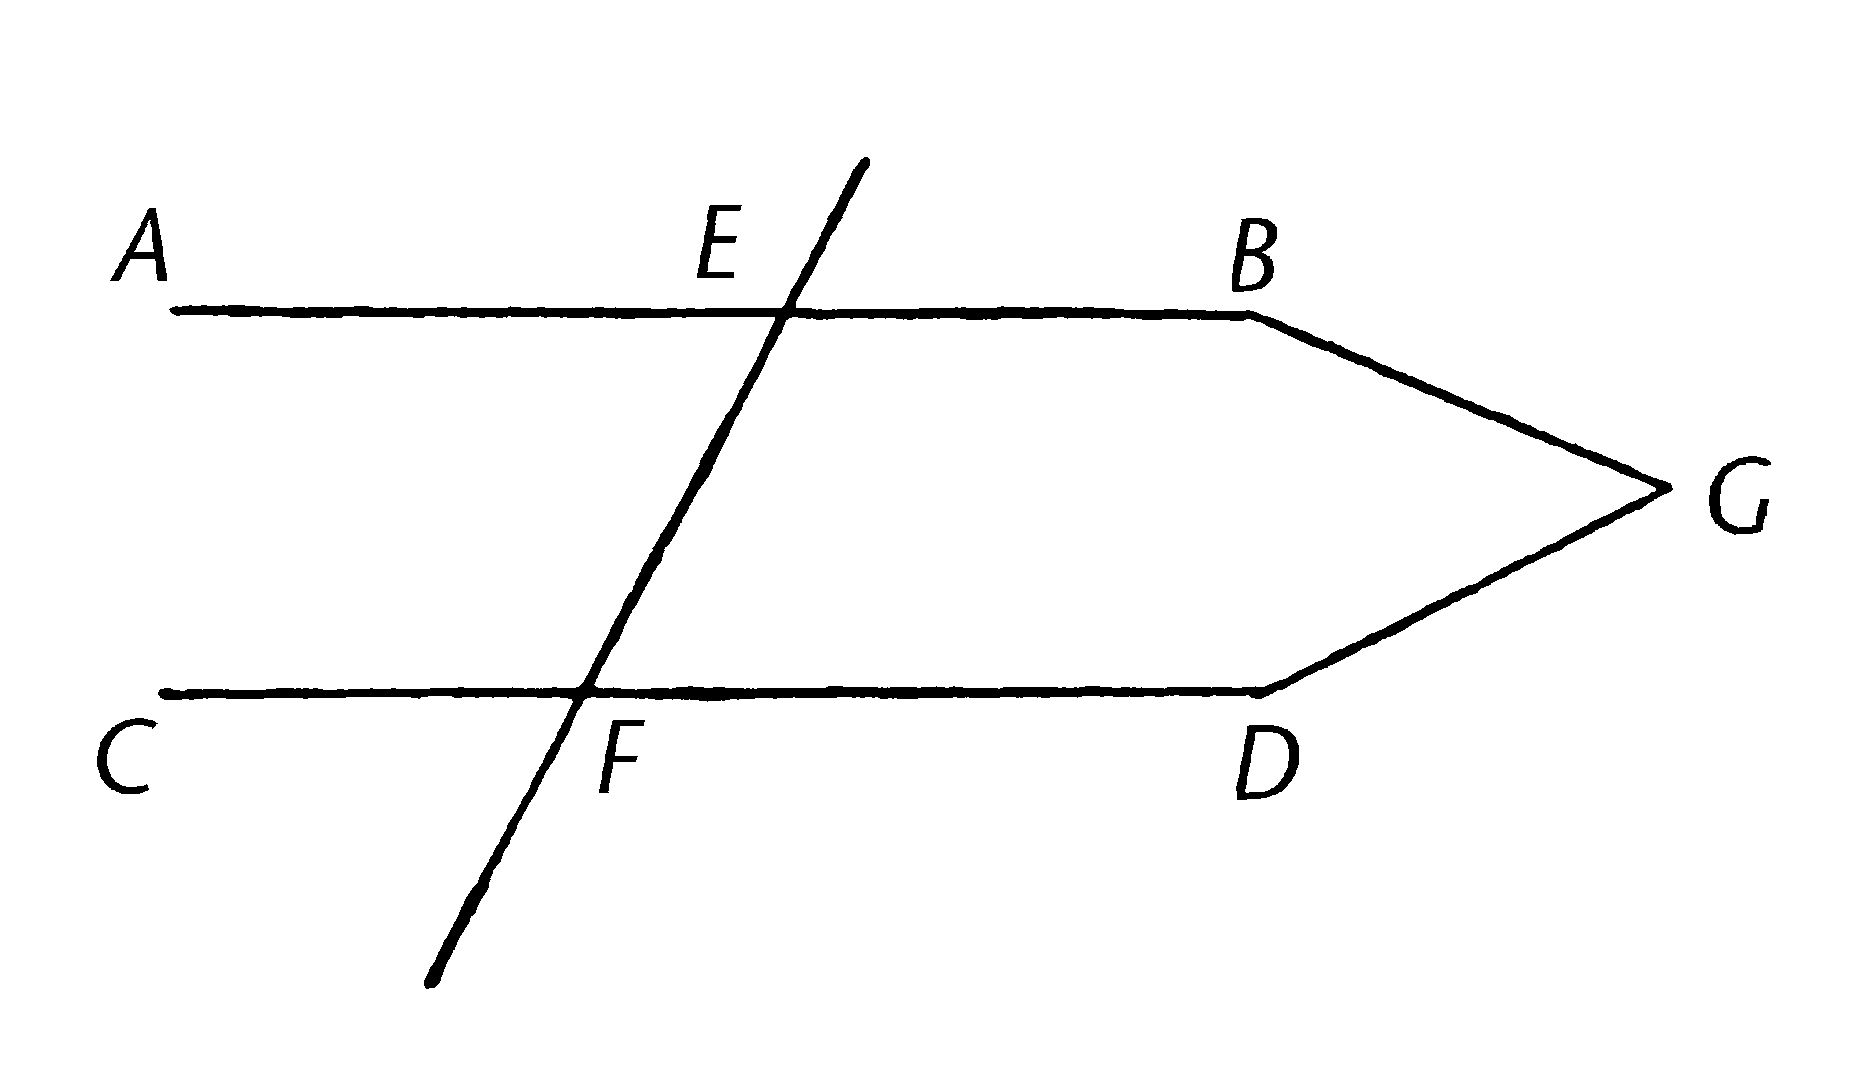
\includegraphics[width=0.5\linewidth]{./image/img508}

作直线EF落于两直线AB,CD上,使得内错角AEF,EFD互等;我说AB平行于CD。

如果不是的话,AB,CD延长时会在B,D或A,C的方向相交。

使它们延长并相交在G,于B,D的方向。

那么,在三角形GEF内,外角AEF等于内错角EFG:这是不可能的。【I.16】

所以AB,CD延长后不会在B,D方向相交。

类似地,可以证明它们也不会在A,C方向相交。

但是两个方向都不相交的直线使平行的【定义23】;所以AB平行于CD。

综上所述\ldots\ldots{}

Q.E.D.

问题示例:

\begin{itemize}
\tightlist
\item
  I.27是我们第一个关于平行的命题,并且它用了归谬法。为什么这个不能直接证明呢?
\item
  定义23说平行线是那些不相交的线;I.27说当内错角相等时,线平行。
\item
  用归谬法,我们假定内错角相等的直线相交。如果它们相交,就被视为与截线构成三角形。
\item
  欧几里得似乎将平行线展示为三角形的一个极端情况?是否有人想过平行线和三角形相关?
\item
  我们能否足够好地画出这个奇怪的假设三角形,来运行证明?当然,我们有一个相反的条件,一个引向归谬法中谬论的设置,但是,如果要确认我们没有被展示着不可能的绘画误导,我们要多小心呢?还是说,这和绘画一点关系都没有,我们只需要保证言语中逻辑步骤的密闭性?
\item
  这个命题和I.16的关系是什么?后者中线相交(给定了三角形)并且证明了内错角不相等。这儿,我们给定了内错角相等并且总结到线是平行的(不相交的)。这个的逻辑关系是什么?我们能从I.16中直接得出么?还是我们必须用归谬法?
\end{itemize}

\hypertarget{ux547dux9898ux4e8cux5341ux516b}{%
\section{命题二十八}\label{ux547dux9898ux4e8cux5341ux516b}}

\textbf{如果一条直线落在两条直线上并使得同位角相等,或者同侧内角和等于两直角,那么两条直线平行。}

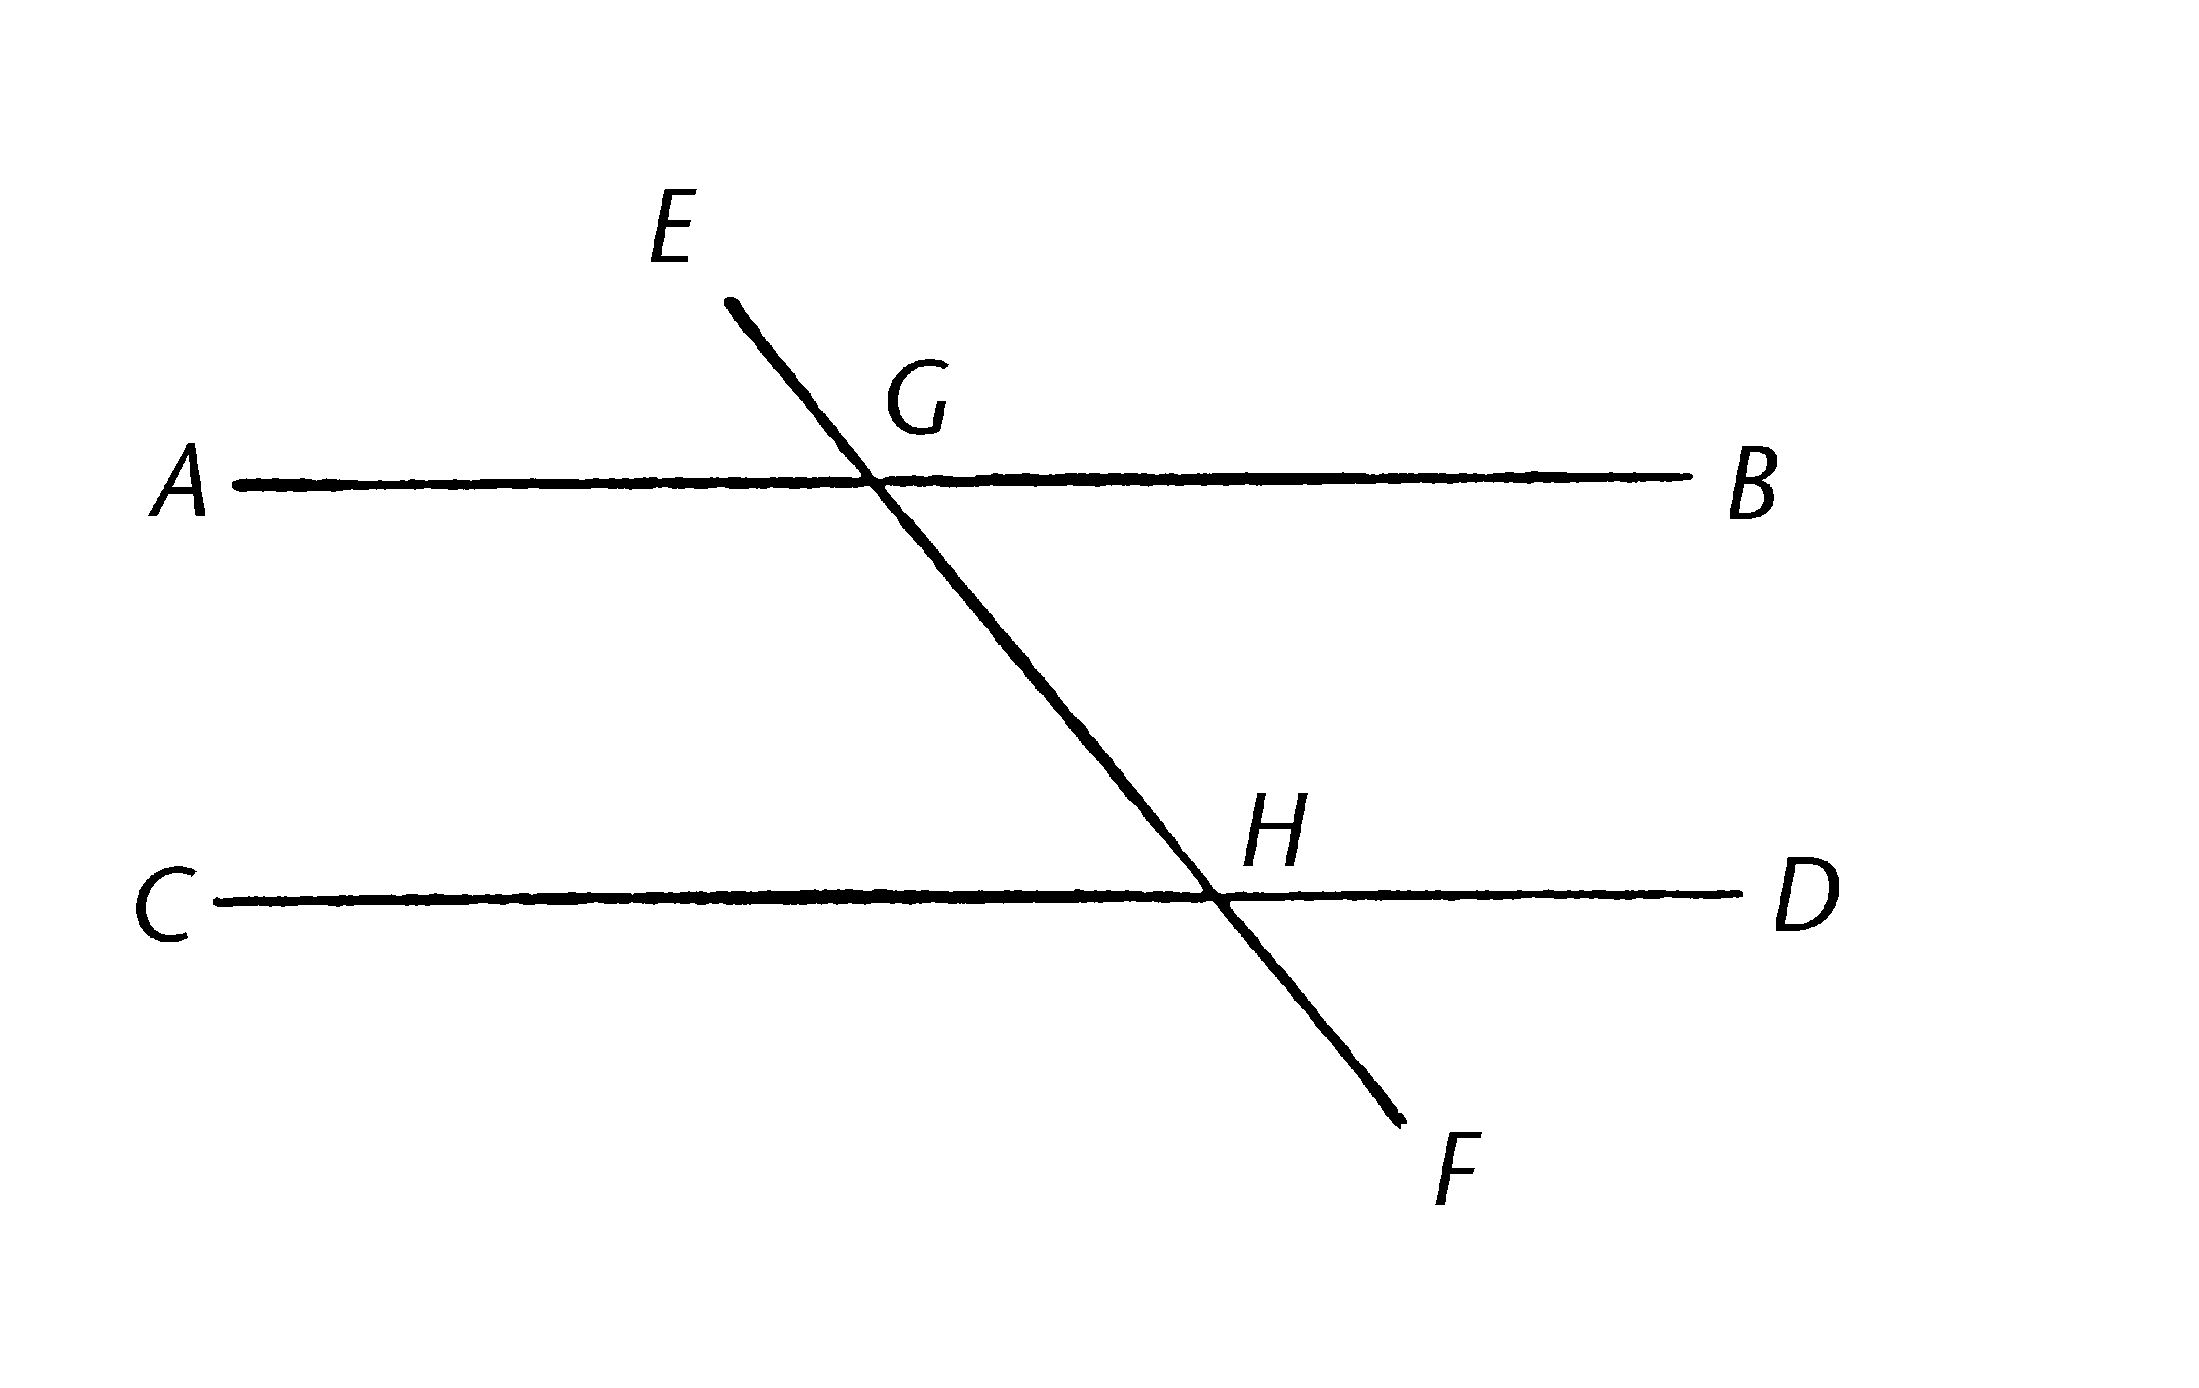
\includegraphics[width=0.5\linewidth]{./image/img511}

作直线EF落于两直线AB,CD上,使得外角EGB等于内错角GHD, 或者同边的内错角,即BGH, GHD等于两直角;我说AB平行于CD。

因为角EGB等于角GHD,当角EGB等于角AGH时【I.15】,角AGH也等于角GHD;并且它们是内错角;所以AB平行于CD【I.27】。

再一次,因为角BGH,GHD等于两直角,且角AGH,BGH也等于两直角【I.13】,角AGH,BGH等于角BGH,GHD。
各自减去角BGH;那么剩余的角AGH等于角GHD;且它们是内错角;所以AB平行于CD【I.27】。

综上所述\ldots\ldots{}

Q.E.D.

【宣棋注:声明中的同位角的原文是the exterior angle 和the exterior angle 这一组角,这里没有直译,而是用了习惯的术语。】

问题示例:

\begin{itemize}
\tightlist
\item
  为什么欧几里得没有将I.28中的两种情况分成两个命题,使三种情况可以通过三个命题来呈现?可能是因为I.27的结论被用于证明I.28中的平行么?
\end{itemize}

\hypertarget{ux547dux9898ux4e8cux5341ux4e5d}{%
\section{命题二十九}\label{ux547dux9898ux4e8cux5341ux4e5d}}

\textbf{落在两平行直线上的直线,会使得内错角互等,同位角互等,同侧内角和等于两直角。}

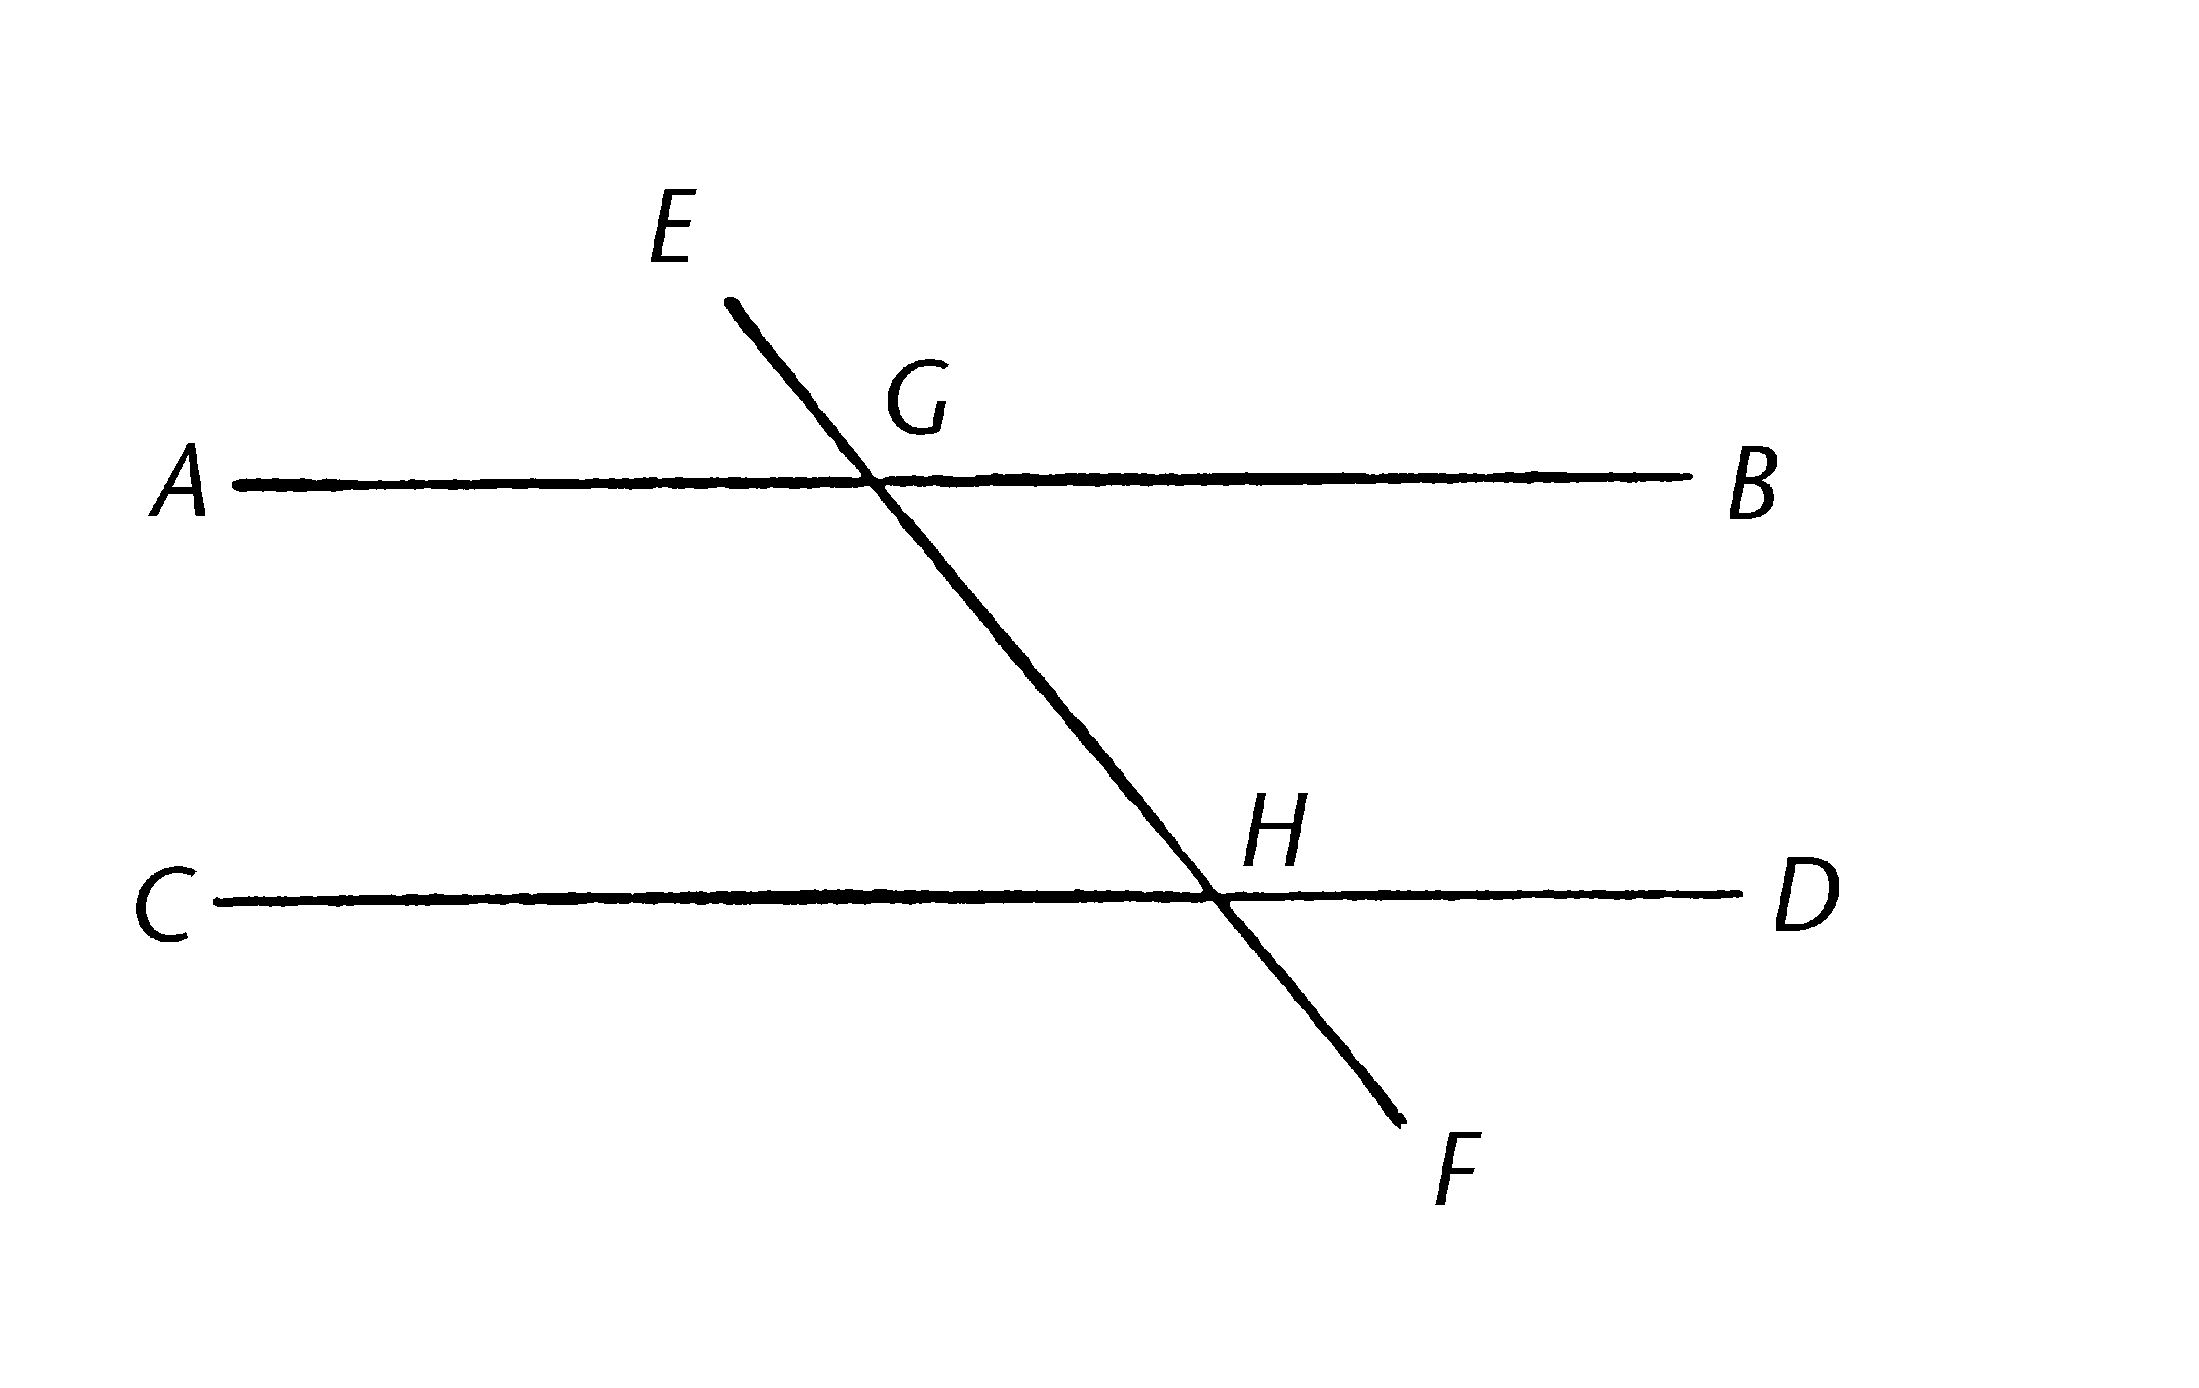
\includegraphics[width=0.5\linewidth]{./image/img511}

作直线EF落于平行直线AB,CD;我说它使得内错角AGH,GHD相等,外角EGB等于内错角GHD,且在同侧的内角,即BGH,GHD等于两直角。

因为,如果角AGH不等于角GHD,那么其中之一会更大。

使角AGH更大。

使各自添加角BGH;所以角AGH,BGH等于两直角【I.13】;所以角BGH.GHD小于两直角。

但是无限延长的直线在角小于两直角的一侧相交【公设5】;

所以AB,CD如果无限延长,就会相交;但是它们不相交,因为它们假设为平行的。所以角AGH不能不等于角GHD,所以它们相等。

再一次,角AGH等于角EGB【I.15】;所以角EGB也等于角GHD【公理1】。

各自添加角BGH;所以角EGB,BGH等于角BGH,GHD【公理2】。

但是角EGB,BGH等于两直角【I.13】;所以角BGH,GHD也等于两直角。

综上所述\ldots\ldots{}

Q.E.D.

问题示例:

\begin{itemize}
\tightlist
\item
  I.29证明了前两个命题的逆命题。为什么我们需要证明它们?
\item
  在确定给定的线平行的逆向条件时,欧几里得第一次调用了公设5,``平行公设''。为什么在这儿的逆条件时,他需要这个公设,但在I.27和I.28中不需要?
\item
  当公设5第一次被提出时,它看起来啰嗦又笨拙。现在,你开始感激它的威力了么?
\item
  公设5使你知道两条延伸的直线会发生什么,通过测量截线落在线上方便绘图的位置的东西。** 这是一个肯定的声明:如果你发现在截线的给定一边上,内角小于两直角,那么线会相交,并且是在这一边。我们没有被要求在脑海里跟随线到无限,以确认它们是否相交,因为我们可能必须做它,如果欧几里得选择了在平行定义基础上的平行假设。
\item
  许多人尝试过改善公设5,或者真正地证明它,但是似乎他们的证明都或多或少暗地里依赖着该假设。你可能被诱惑着开始尝试独立证明这个假设,而且你已经有前29个命题作为工具。在这个棘手的地方,甚至许多伟大的人曾经倒下,但是尽管最终失败了,付出的努力本身会是有趣且富有启发性的。
\end{itemize}

\hypertarget{ux547dux9898ux4e09ux5341}{%
\section{命题三十}\label{ux547dux9898ux4e09ux5341}}

\textbf{与同一直线平行的直线们,也互相平行。}

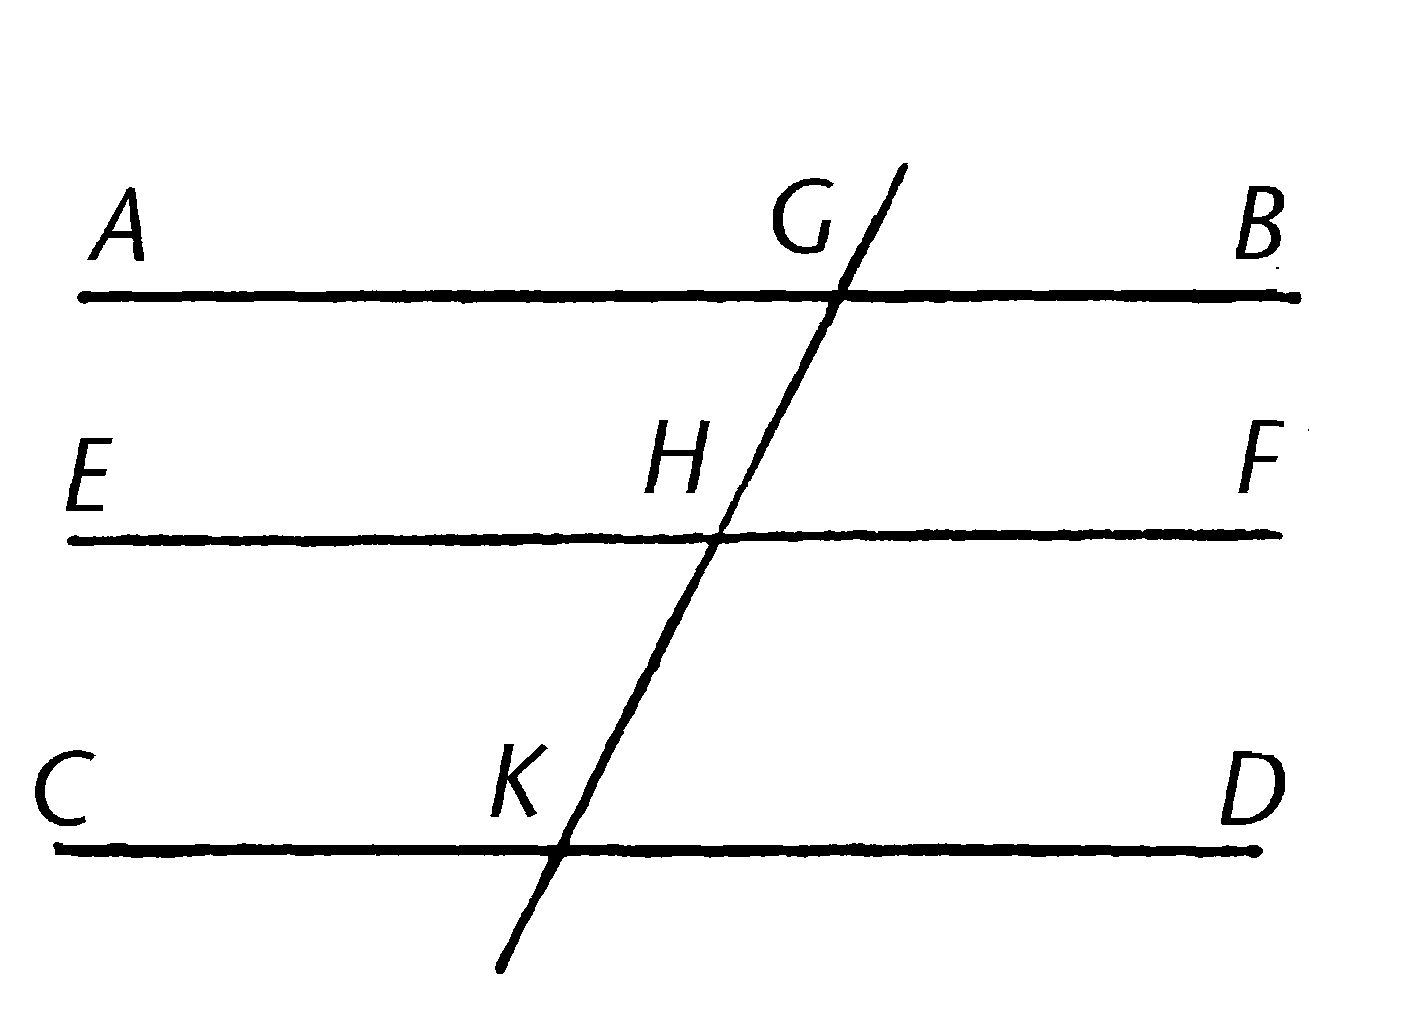
\includegraphics[width=0.3\linewidth]{./image/img515}

使直线AB,CD均平行于EF; 我说AB也平行于CD。

使直线GK落在它们上。

因为直线GK落在了平行直线AB,EF上, 角AGK等于角GHF【I.29】。

再一次,因为直线GK落在了平行直线EF,CD上,角GHF等于角GKD【I.29】。

但是已证明角AGK等于角GHF;所以角AGK也等于角GKD【公理1】; 且它们使内错角。

所以AB平行于CD。

Q.E.D.

【宣棋注:思考为什么这里省略了''综上所述\ldots``?】

\hypertarget{ux547dux9898ux4e09ux5341ux4e00}{%
\section{命题三十一}\label{ux547dux9898ux4e09ux5341ux4e00}}

\textbf{过定点,画一条直线,使平行于另一条直线。}

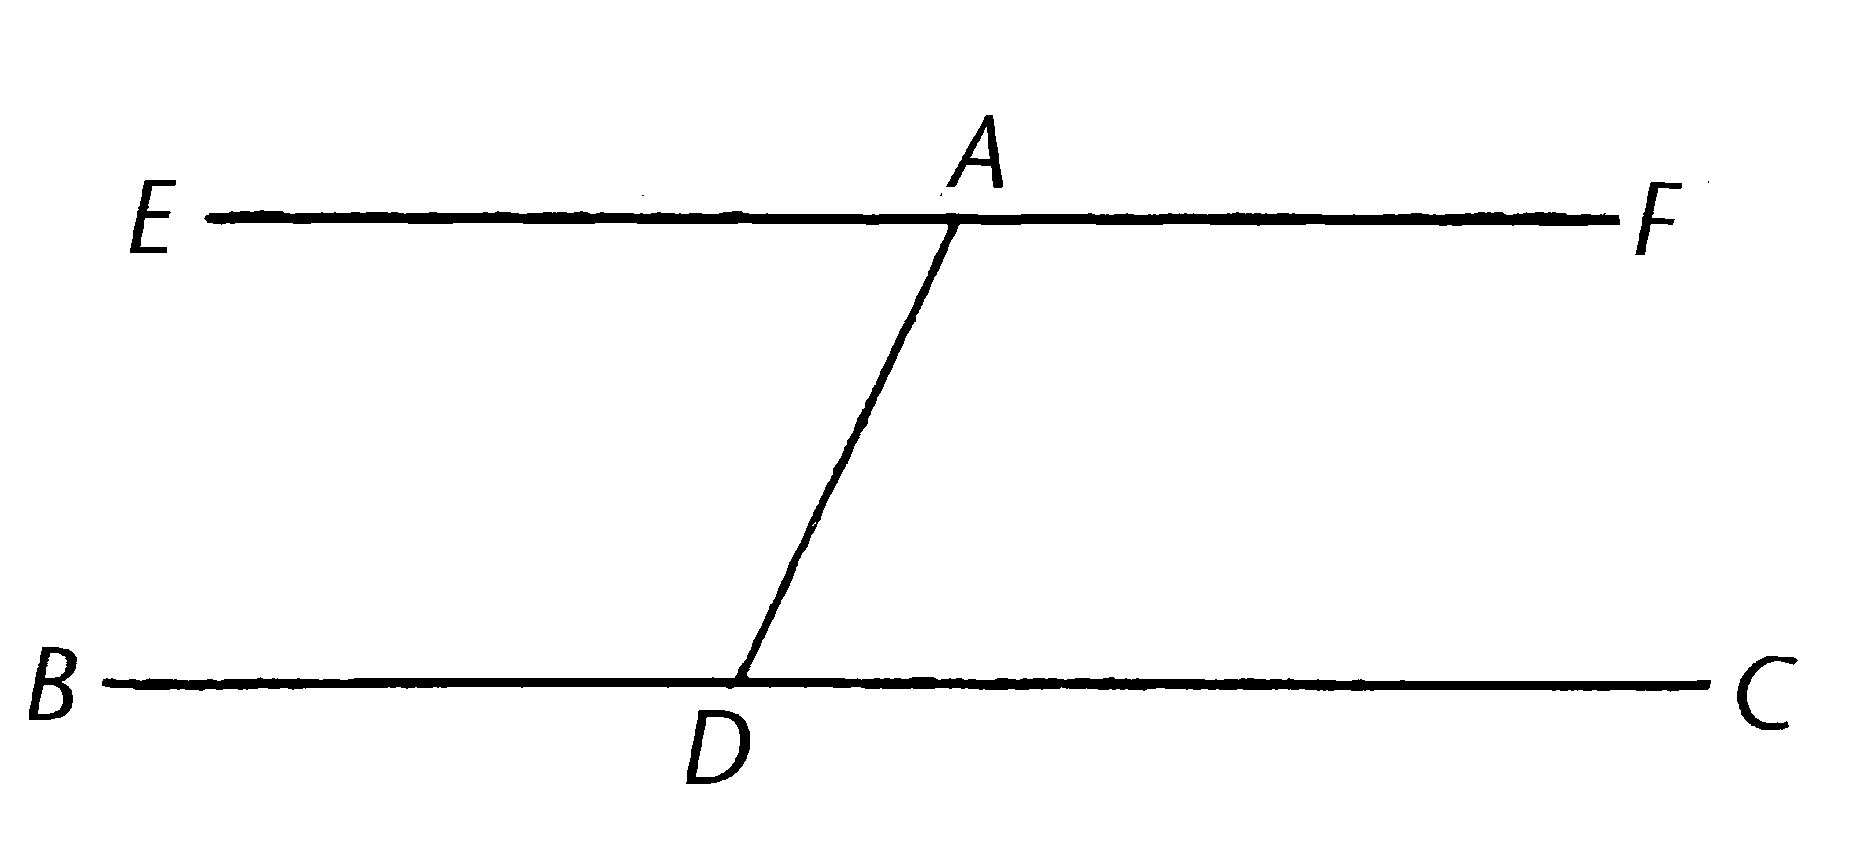
\includegraphics[width=0.3\linewidth]{./image/img517}

使点A为给定点,BC为给定直线;那么需要从点A画直线平行于直线BC。

在BC上任意取点D,且连接AD;在直线DA的点A上,构建角DAE,使等于角ADC【I.23】;且在EA上延长直线AF。

那么,因为直线AF落在两直线BC,EF上使得内错角EAD,ADC互等,那么EAF平行于BC【I.27】。

所以过点A,画直线EAF平行于给定直线BC。

Q.E.F.

问题示例:

\begin{itemize}
\tightlist
\item
  这是否暗示或者奠定了:过任意一点,只能有一条直线平行于给定直线?这能告诉我们关于平行的什么呢?因为这个命题似乎只调用了那些涉及公设五之前部分的命题,这个命题能被用来替换公设五么?或者说I.30的思考(依赖于公设五)对于``只有一种平行''的性质是必须的?
\end{itemize}

\hypertarget{ux547dux9898ux4e09ux5341ux4e8c}{%
\section{命题三十二}\label{ux547dux9898ux4e09ux5341ux4e8c}}

\textbf{在任意三角形中,如果延长一边,那么外角等于两内对角之和,且三个内角的和等于两直角。}

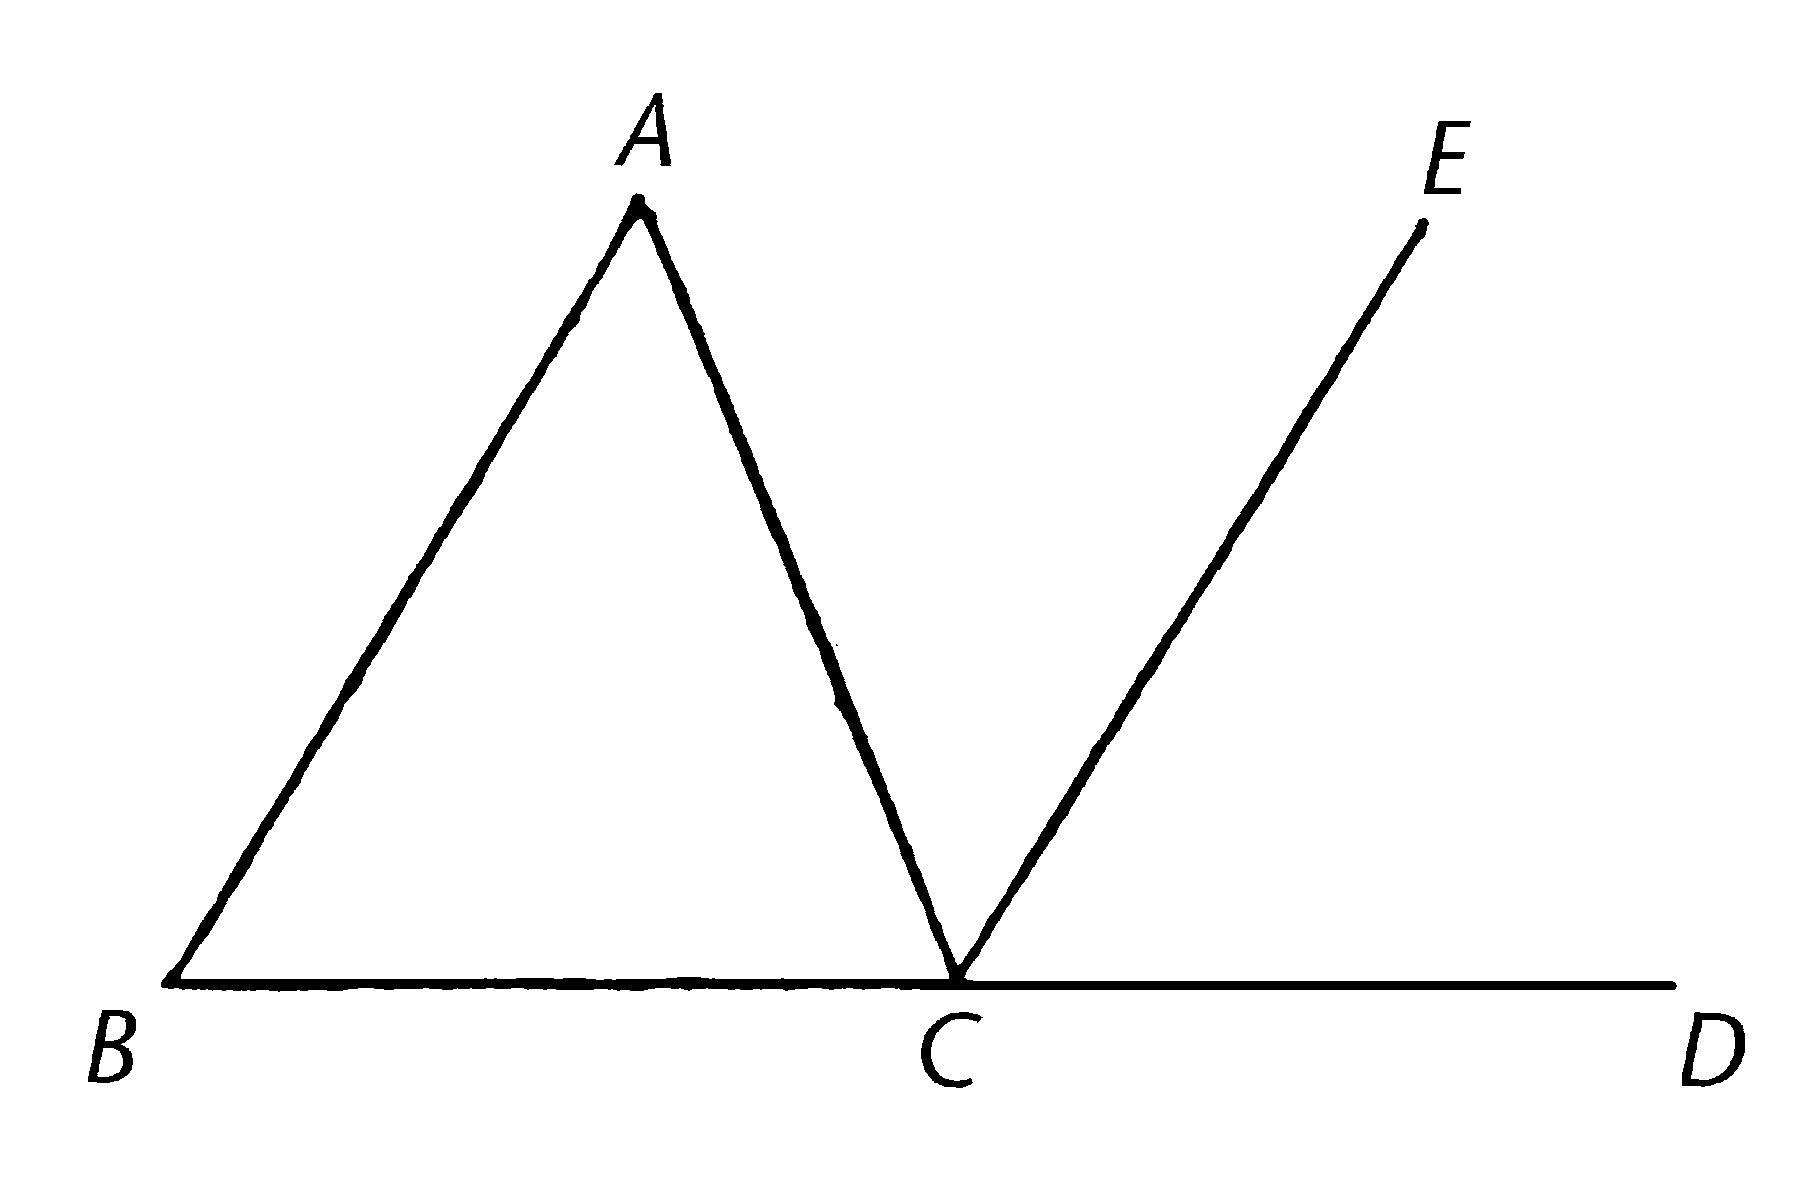
\includegraphics[width=0.3\linewidth]{./image/img519}

给定三角形ABC,并延长其中一边BC至D;我说外角ACD等于两个内对角CAB,ABC,且三角形三个内角ABC,BCA,CAB等于两直角。

过点C画CE,使平行于直线AB。

那么,因为AB平行于CE,且AC落于它们之上,内错角BAC,ACE互等【I.29】。

再一次,因为AB平行于CE,且直线BD落于它们之上,外角ECD等于内对角ABC【I.29】。

但是已证明角ACE等于角BAC;所以整角ACD等于两内对角BAC,ABC。

各自添加角ACB;所以角ACD,ACB等于三个角ABC,BCA,CAB。

但是角ACD,ACB等于两直角【I.13】; 所以角ABC,BCA,CAB也等于两直角。

综上所述\ldots\ldots{}

Q.E.D.

问题示例:

\begin{itemize}
\tightlist
\item
  回到I.17,我们证明了三角形内任意两角之和小于两直角。为什么欧几里得先证明了这个较弱的形式,而之后(也就是现在)才证明内角和等于两直角?我们有感觉到他试图在不调用公设5的情况下证明尽可能多的的命题吗?为什么会这样呢?
\item
  现在,我们是不是有了更简单证明I.26所需要的内容?但是,再一次,这会不会很重要呢------欧几里得似乎希望能不用那些依赖于公设5的命题来证明I.26?
\end{itemize}

\hypertarget{ux547dux9898ux4e09ux5341ux4e09}{%
\section{命题三十三}\label{ux547dux9898ux4e09ux5341ux4e09}}

\textbf{向同一方向「分别」连接相等且平行线段「端点」的线段也相等且平行。}

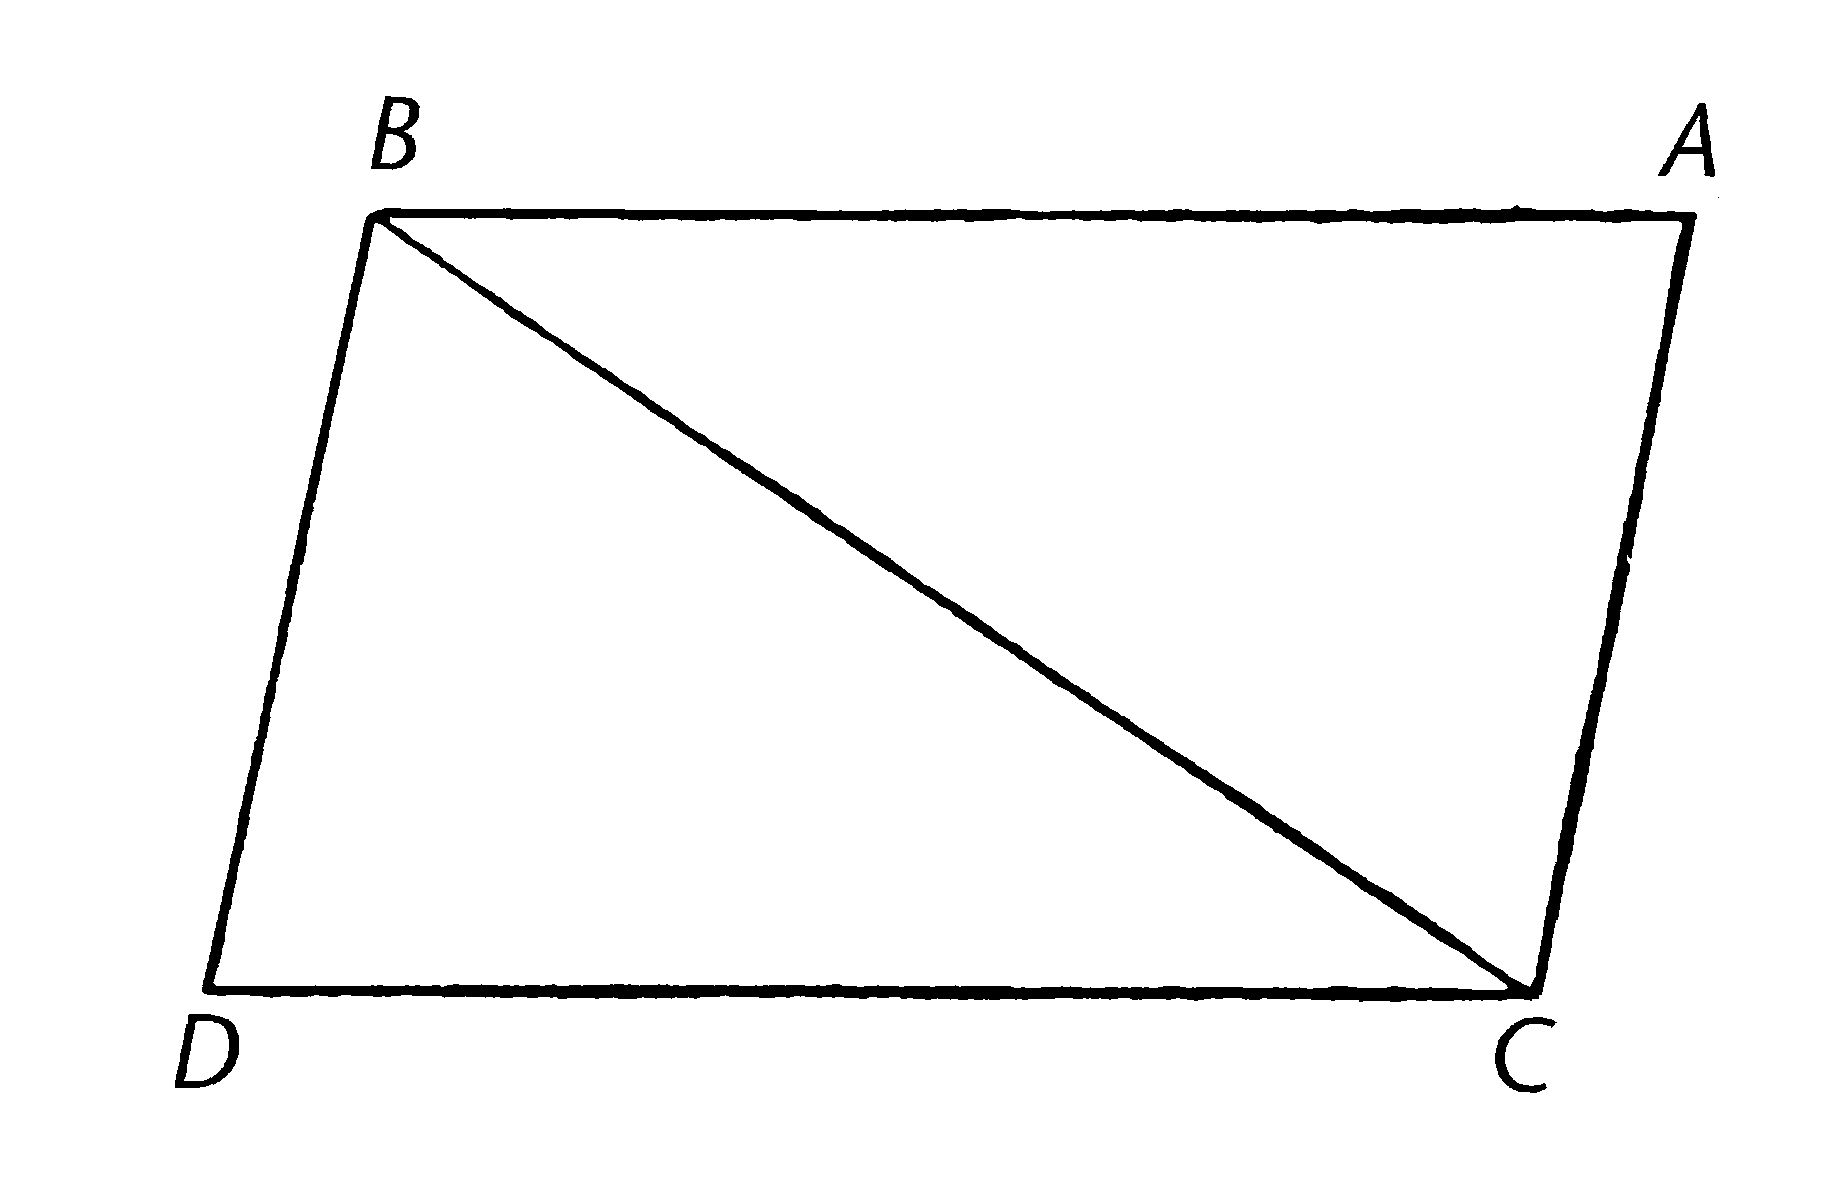
\includegraphics[width=0.3\linewidth]{./image/img521}

使AB,CD相等且平行,并{[}从其端点{]}向同方向分别连接直线AC,BD;我说AC,BD也互相相等且平行。

连接BC。

那么,因为AB平行于CD,且BC落在它们上面,内角ABC,BCD互等【I.29】。

且因为AB等于CD,且BC是共有的,两边AB,BC等于两边DC,CB;且角ABC等于角BCD;所以底边AC等于底边BD,且三角形ABC全等于三角形DCB,且剩余的角各自互等,即等边所对的角【I.4】;所以角ACB等于角CBD。

又因为落在两直线AC,BD上的直线BC使得内错角互等,AC平行于BD【I.27】。

且已证明它们相等。

综上所述\ldots\ldots{}

Q.E.D.

问题示例:

\begin{itemize}
\tightlist
\item
  尽管这个命题并没有声明这是构建一个``平行四边形的区域'',事实上接下来的命题会用这个术语并使我们意识到,我们已经构建了这个图形。命名了一些四边形的定义22却没有提及这个。所以现在我们既有一个隐含的定义,又有一个存在的证明(一个可以被构建的论证以及它的构建)?为什么欧几里得没有在定义22中包含平行四边形?是因为他还没有定义平行线(在定义23中完成)么?还有没有其它原因导致欧几里得推迟了对平行线的处理?
\end{itemize}

\hypertarget{ux547dux9898ux4e09ux5341ux56db}{%
\section{命题三十四}\label{ux547dux9898ux4e09ux5341ux56db}}

\textbf{在平行四边形的区域内,对边及对角互等,且对角线平分该区域。}

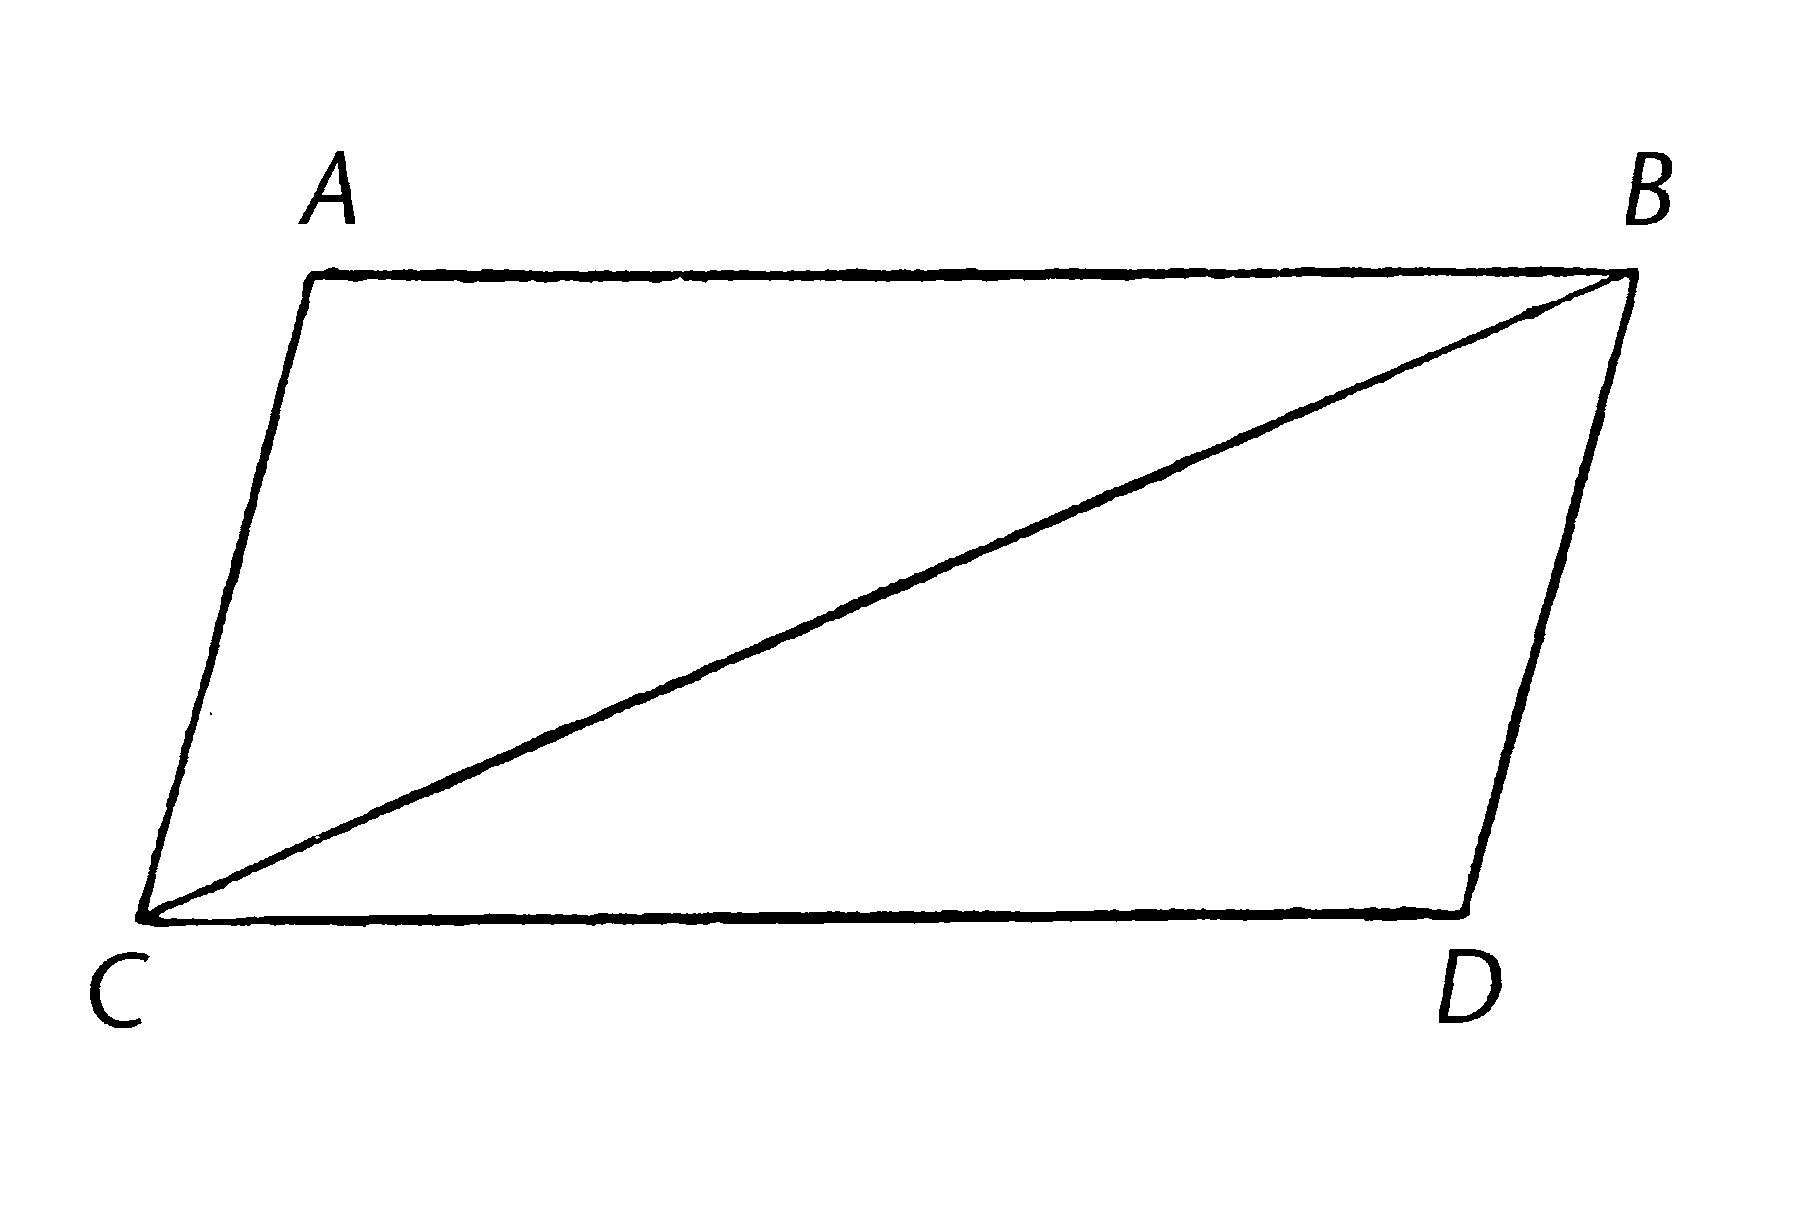
\includegraphics[width=0.3\linewidth]{./image/img523}

给定平行四边形的区域ACDB,且BC是其对角线;我说平行四边形ACDB的对边和角互等,且对角线BC将其平分。

因为AB平行于CD,且直线BC落在它们上,内错角ABC,BCD互等【I.29】。

再一次,因为AC平行于BD,且BC落在它们上,内错角ACB,CBD互等【I.29】。

所以三角形ABC,DCB中两角ABC,BCA分别与两角DCB,CBD互等,且一边互等,即连接两等角并共有的边,BC;所以它们剩余的边和角也各自互等【I.26】;所以边AB等于CD,AC等于BD,且角BAC等于角CDB。

又因为角ABC等于角BCD,且角CBD等于角ACB,整角ABD等于整角ACD【公理2】。

且已证明角BAC等于角CDB。

所以在平行四边形的区域中,对边对角互等。

我说,接下来,对角线将区域平分。

因为AB等于CD,且BC是共有的,两边AB,BC分别等于两边DC,CB;且角ABC等于角BCD;所以底边AC等于DB,且三角形ABC全等于三角形DCB。【I.4】

所以对角线BC平分平行四边形ACDB。

【宣棋注:这里的对角线英文也是``diameter''同圆的直径,翻译成对角线以适应一般习惯。】

问题示例:

\begin{itemize}
\tightlist
\item
  关于我们能在区域相等上知道什么,你是否一直在跟踪它的发展?到目前为止,我们仅仅涉及三角形,I.4明确做的全等三角形(三角形可以被移动并且放置到与他们重合的三角形上),通过应用I.4,I.8和I.26也引到了相同的结论。
\item
  现在我们前行到其它图形,并且很快就要将这个关于重合的黄金法则抛之脑后了。但是这个命题有做比试探更多的事情么?平行四边形被分割成两个全等三角形,通过I.4可知它们相等,所以我们总结到这个平行四边形的区域被平分了。
\item
  我们是否通过另一种方式迈上了新台阶?这是第一次,欧几里得以命题的形式明确地平分一个区域。在证明上,(也就是说不考虑定义17中关于平分圆的声明)我们之前平分了角和线。现在,我们平分了一个区域。但是在I.9通过构建全等的直角三角形来平分角的时候,我们是不是已经隐含着平分了区域?
\item
  在这个命题中,欧几里得谈论了``平行四边形的区域'';这是他用到这个术语area (\ldots\ldots)的唯一一个地方。区域一词并没有出现在其它任何地方(引用这个命题的语句除外)。区域也没有被定义。(定义5是关于面的,面是只有长度和宽度的。)但是这儿,在命题34的第二部分,直径平分区域时,看起来在说图形的尺寸,或者图形里关于区域的关系。所以,什么是区域?是关于它的尺寸和尺寸的比较么?还是更多的关于所占有的空间(内容,图形的本体)?
\item
  这些图形是我们称为空间或者面的那些大的消耗中分理出的部分么?还是说,从一个图形可以等于其它事物的角度看,它们有独立存在的权利,从其它他们可能依附的那些连续事物中?
\end{itemize}

\hypertarget{ux547dux9898ux4e09ux5341ux4e94}{%
\section{命题三十五}\label{ux547dux9898ux4e09ux5341ux4e94}}

\textbf{同底且在同组平行线之间的平行四边形互等。}

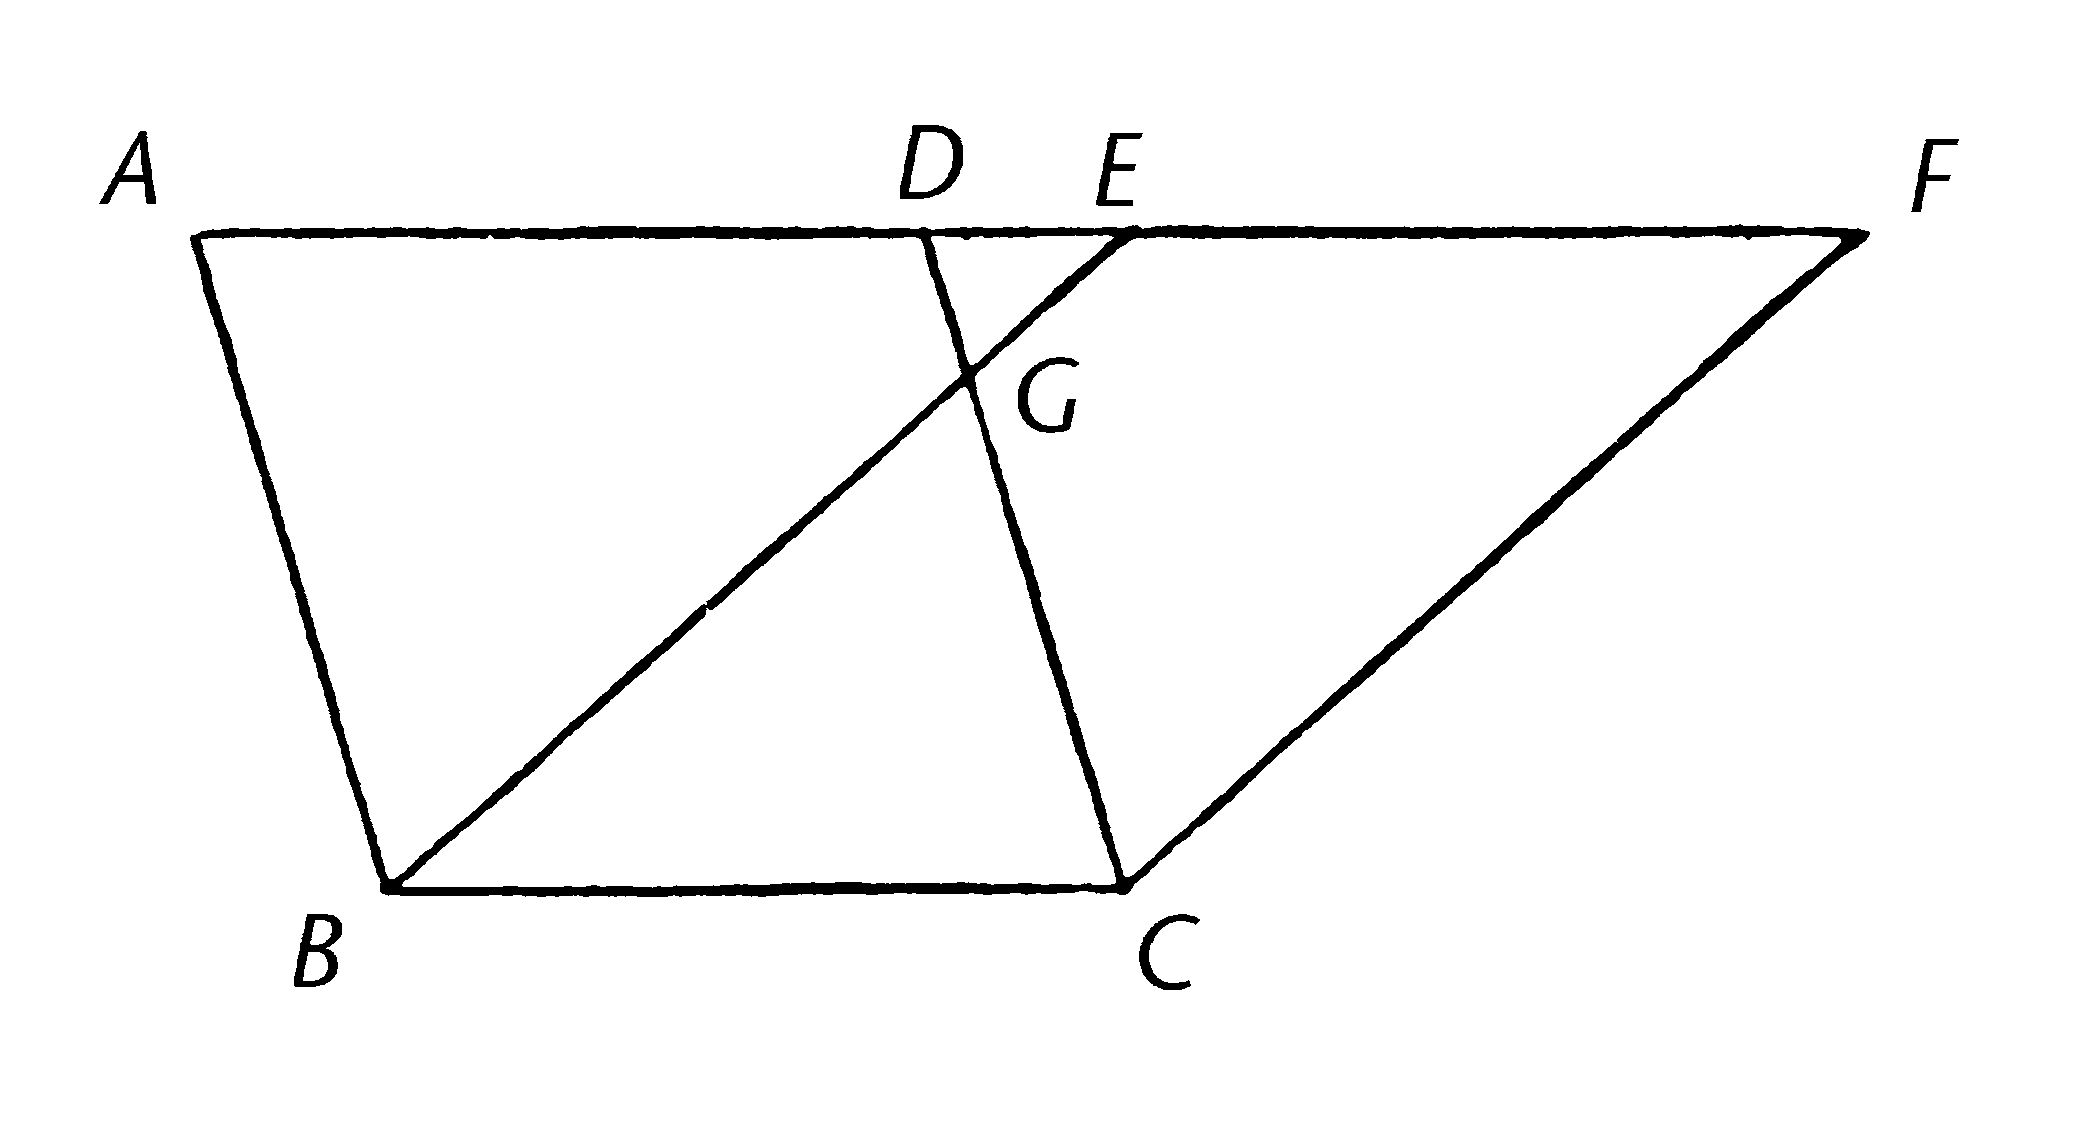
\includegraphics[width=0.5\linewidth]{./image/img526}

ABCD,EBCF是同底边BC上的平行四边形,且在同平行线AF,BC之间;我说ABCD等于平行四边形EBCF。

因为ABCD是平行四边形,AD等于BC。【I.34】

同理可得EF等于BC,所以AD也等于EF【公理1】;且DE是共有的;所以整个AE等于整个DF。【公理2】

但是AB也等于DC【I.34】;所以两边EA,AB分别等于两边FD,DC,且同位外角FDC等于同位内角EAB【I.29】;所以底边EB等于底边FC,且三角形EAB也全等于三角形FDC【I.4】。

各自减去DGE;所以剩余的不规则四边形ABGD等于剩余的不规则四边形EGCF。【公理3】

各自添加三角形GBC;所以整个平行四边形ABCD等于整个平行四边形EBCF。

综上所述\ldots\ldots{}

Q.E.D.

问题示例:

\begin{itemize}
\tightlist
\item
  到目前为止,所有我们被告知相等的事物(比如说公设4中``所有的直角''),以及所有我们已证明相等的事物(各种全等三角形),都是在公理4中命名的那种相等,即彼此重合的事物相等。
\item
  但是我们真的知道相等性是什么吗?欧几里得从未定义过相等性。它是我们应该已经了解的事物么?我们在一开始被告知过这些:公理给予我们一些性质,特别是重合的事物相等。确实我们可以把这个作为相等是什么的定义。
\item
  我们广泛地研究了相等的三角形。现在我们超越了三角形,且在证明平行四边形的相等性。但是,等一下!所有的相等三角形是可以被放置成重合的。这些在命题I.35中声明为相等平行四边形的不可以!
\item
  从一致性和重合性到不同形状图形的相等性的推进是什么?
  现在我们如何理解相等性?我们必须开始用新的思想上关于相等性的定义,来锻造新的图景。是否把这些空间切成能通过I.4证明相等的三角形,还有通过公理证明有用的加减三角形,直到我们能够有逻辑的展示出图形是被相同部分组成的?**这似乎是这个命题运用的方式。这会成为我们新的定义么?给这新的相等性取一个新的名字,会有帮助么?
\item
  不同的形状可以被证明相等,这令人感到惊讶么?想象图像中,EF在右边很远的举例,一个近乎无限长的狭窄的图形。这个图形的周长肯能到达无限,然后我们发现这个区域和一个矮胖的平行四边形相同,可能是个正方形,在同样的底上。是这样的事物使得几何学的研究获得了直觉无法获得的关于真理产生的赞誉么?
\item
  你是否对自己能发现全等三角形有所期待,或许通过对其它三角形的一些简单操作,并得到你的证明?到目前为止,仔细而系统搭建的工具,以及最近以平行假设为基础命题的力量,使得它看起来变得简单了。
\item
  你之前有用挑剔的目光看待你在开发的绘图的构建么?如果EF和AD重合,论证会有什么不同?欧几里得是不是又一次选择了最难的情况?
\item
  证明这个命题,你是否之前有看到过其它你可能在这个绘图中实现的操纵三角形的方式?比如说,通过选择不同的全等三角形,你能够通过在全等三角形上加一个三角形,而不是既加又减来实现它?你能找到一个适用于所有情况的证明么?
\item
  这里是不是还隐藏了另一项发展?我们依据公理:从相等的量添加或减少相等的量后始终相等。当一个对应的部分被添加或者减少时,这些似乎确实值得被称为几何公理,例如在两个全等三角形一角上(放置在对应角上)的一个小三角形。但是这是第一次我们没有添加或者减少相对应的部分么?我们添加或减少的等量是各个图形不同的部分。这个产生相等性是不是一个暗含的假设,还是说这是我们可以假定理解其合法性的事物,且在公理2和3之中已经充分阐释了?**
\end{itemize}

**【宣棋注1:英文中的''trapezium''对应的前文定义22中最后的``trapezia'',所以在这里翻译成不规则四边形,而没有翻译成梯形。】

**【宣棋注2:在英文文本里,三角形全等的原文其实是``triangle \ldots is equal to triangle \ldots'', 而不规则四边形的也是 ``trapezium \ldots is equal to trapezium \ldots{}'',但是这里没有翻译成全等,只是翻译为等于,原因正是在问题示例中所提及的,这种未经证明可以重合放置的相等是同一类的相等么?】

\hypertarget{ux547dux9898ux4e09ux5341ux516d}{%
\section{命题三十六}\label{ux547dux9898ux4e09ux5341ux516d}}

\textbf{等底且在同组平行线之间的平行四边形互等。}

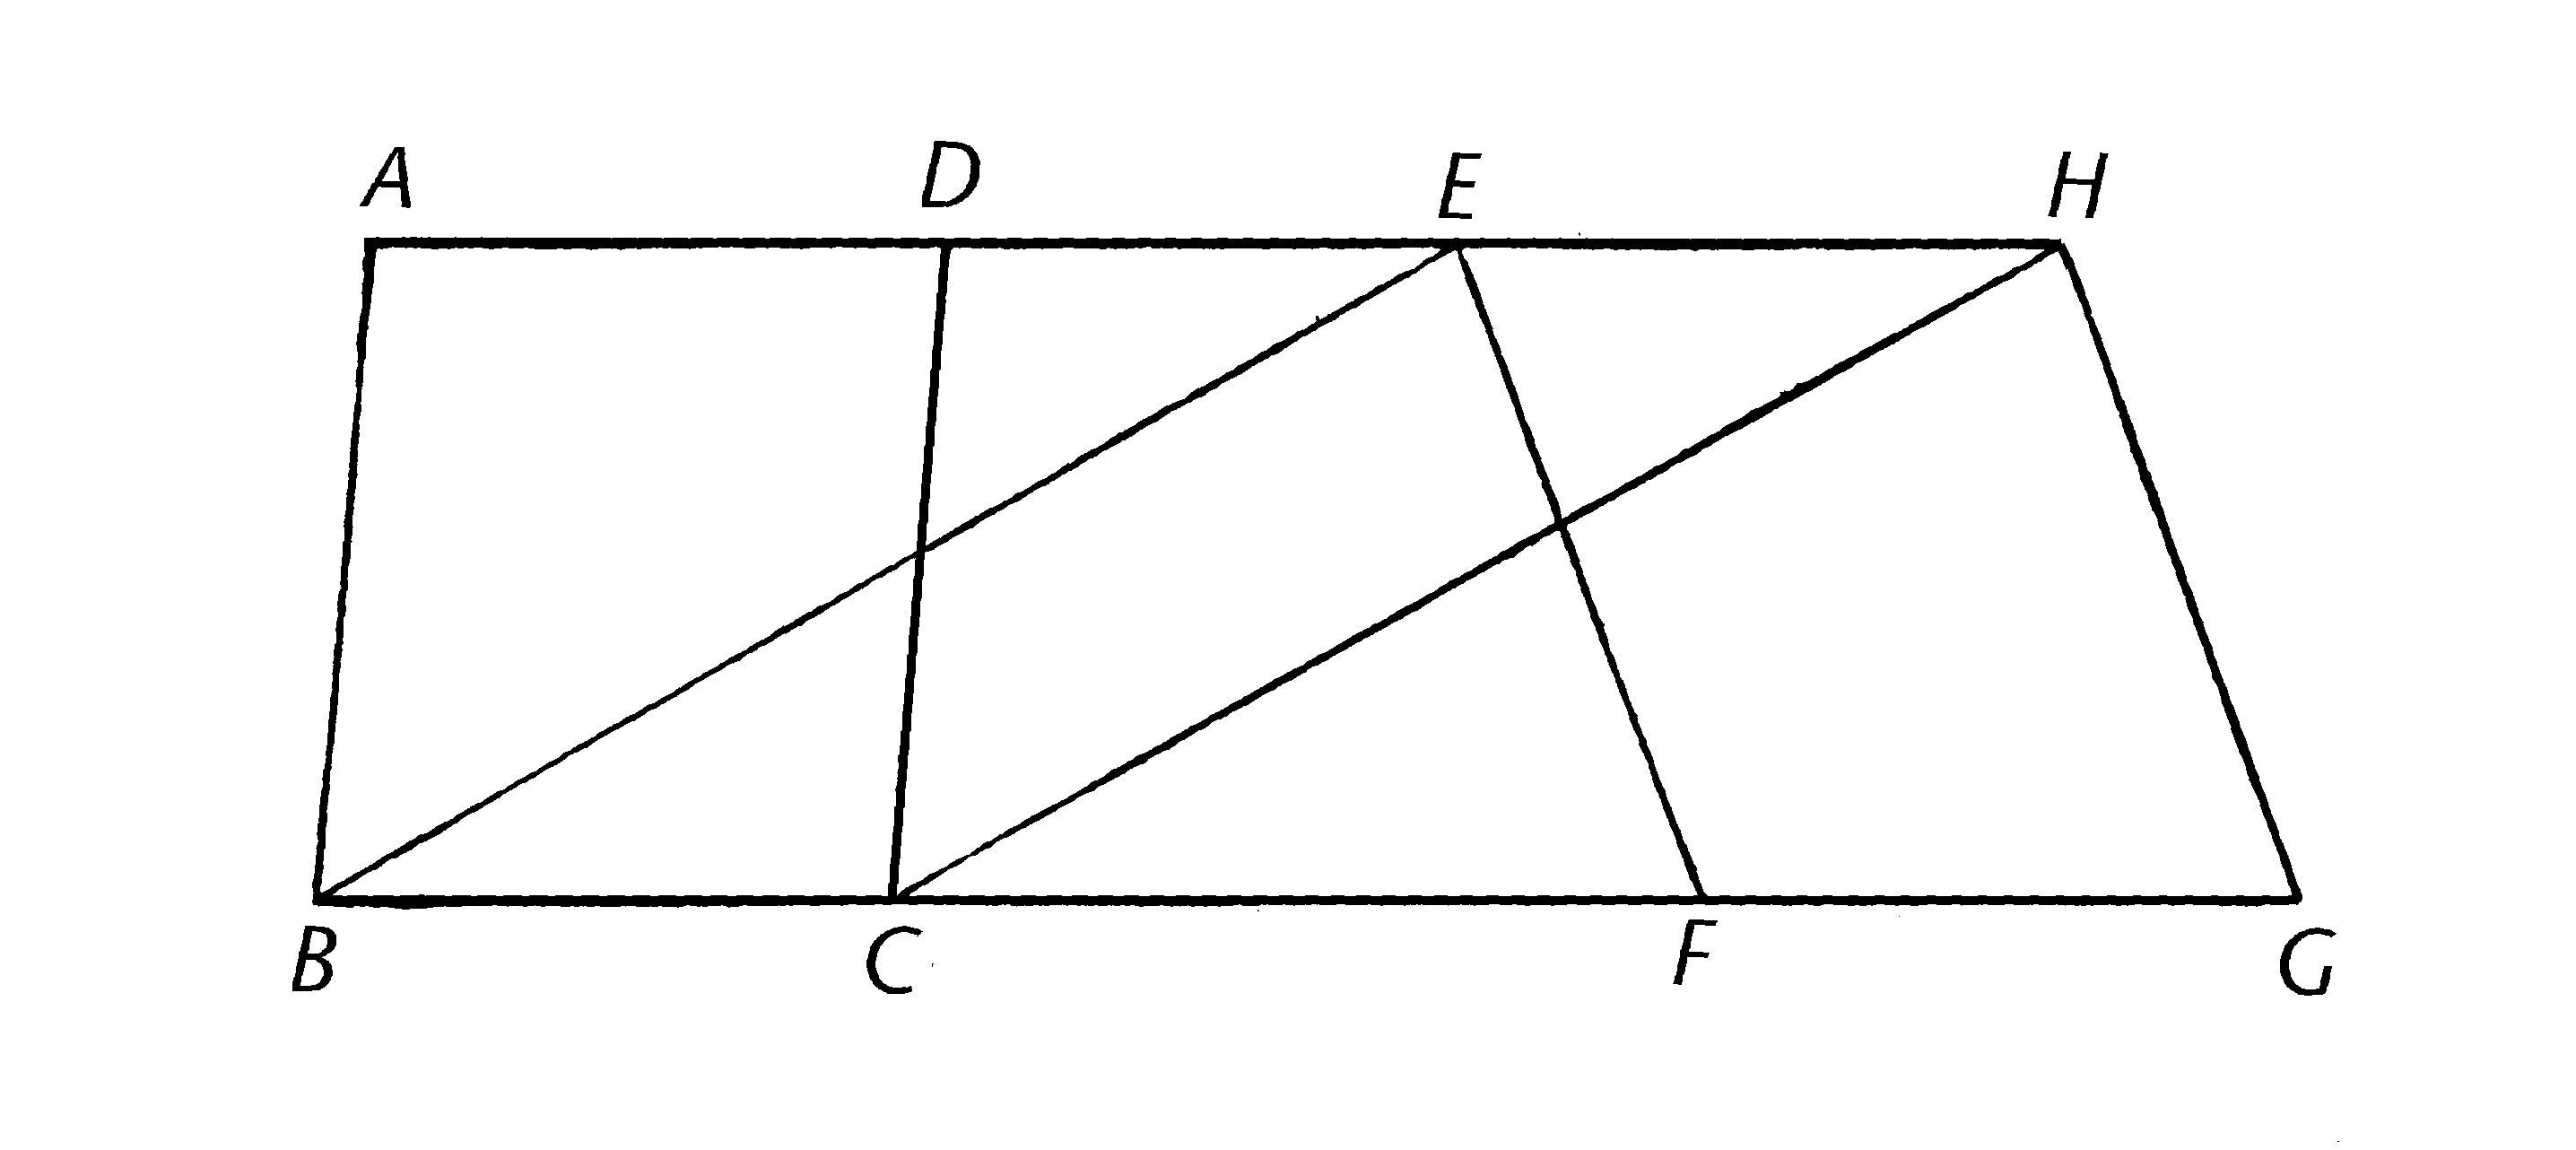
\includegraphics[width=0.5\linewidth]{./image/img530}

ABCD, EFGH是在等底BC, FG上的平行四边形,且在同平行线BC,FG之间;我说平行四边形ABCD等于EFGH。

连接BE,CH。

那么,因为BC等于FG,而FG等于EH,BC也等于EH 。【公理1】

但它们也平行。

连接EB,HC;但向同一方向「分别」连接相等且平行线段「端点」的线段也相等且平行。【I.33】

所以EBCH是平行四边形。【I.34】

且它也等于ABCD;因为它与BC同底,且在相同的平行线BC,AH之间。【I.35】

同理可得,EFGH也等于EBCH【I.35】;所以平行四边形ABCD也等于EFGH。【公理1】

综上所述\ldots\ldots{}

Q.E.D.

问题示例:

\begin{itemize}
\tightlist
\item
  现在平行四边形已经无需同底,只需等底!你是否看到面积的相等性正在日益增长的从重合中脱离?
\end{itemize}

\hypertarget{ux547dux9898ux4e09ux5341ux4e03}{%
\section{命题三十七}\label{ux547dux9898ux4e09ux5341ux4e03}}

\textbf{同底且在同组平行线之间的三角形互等。}

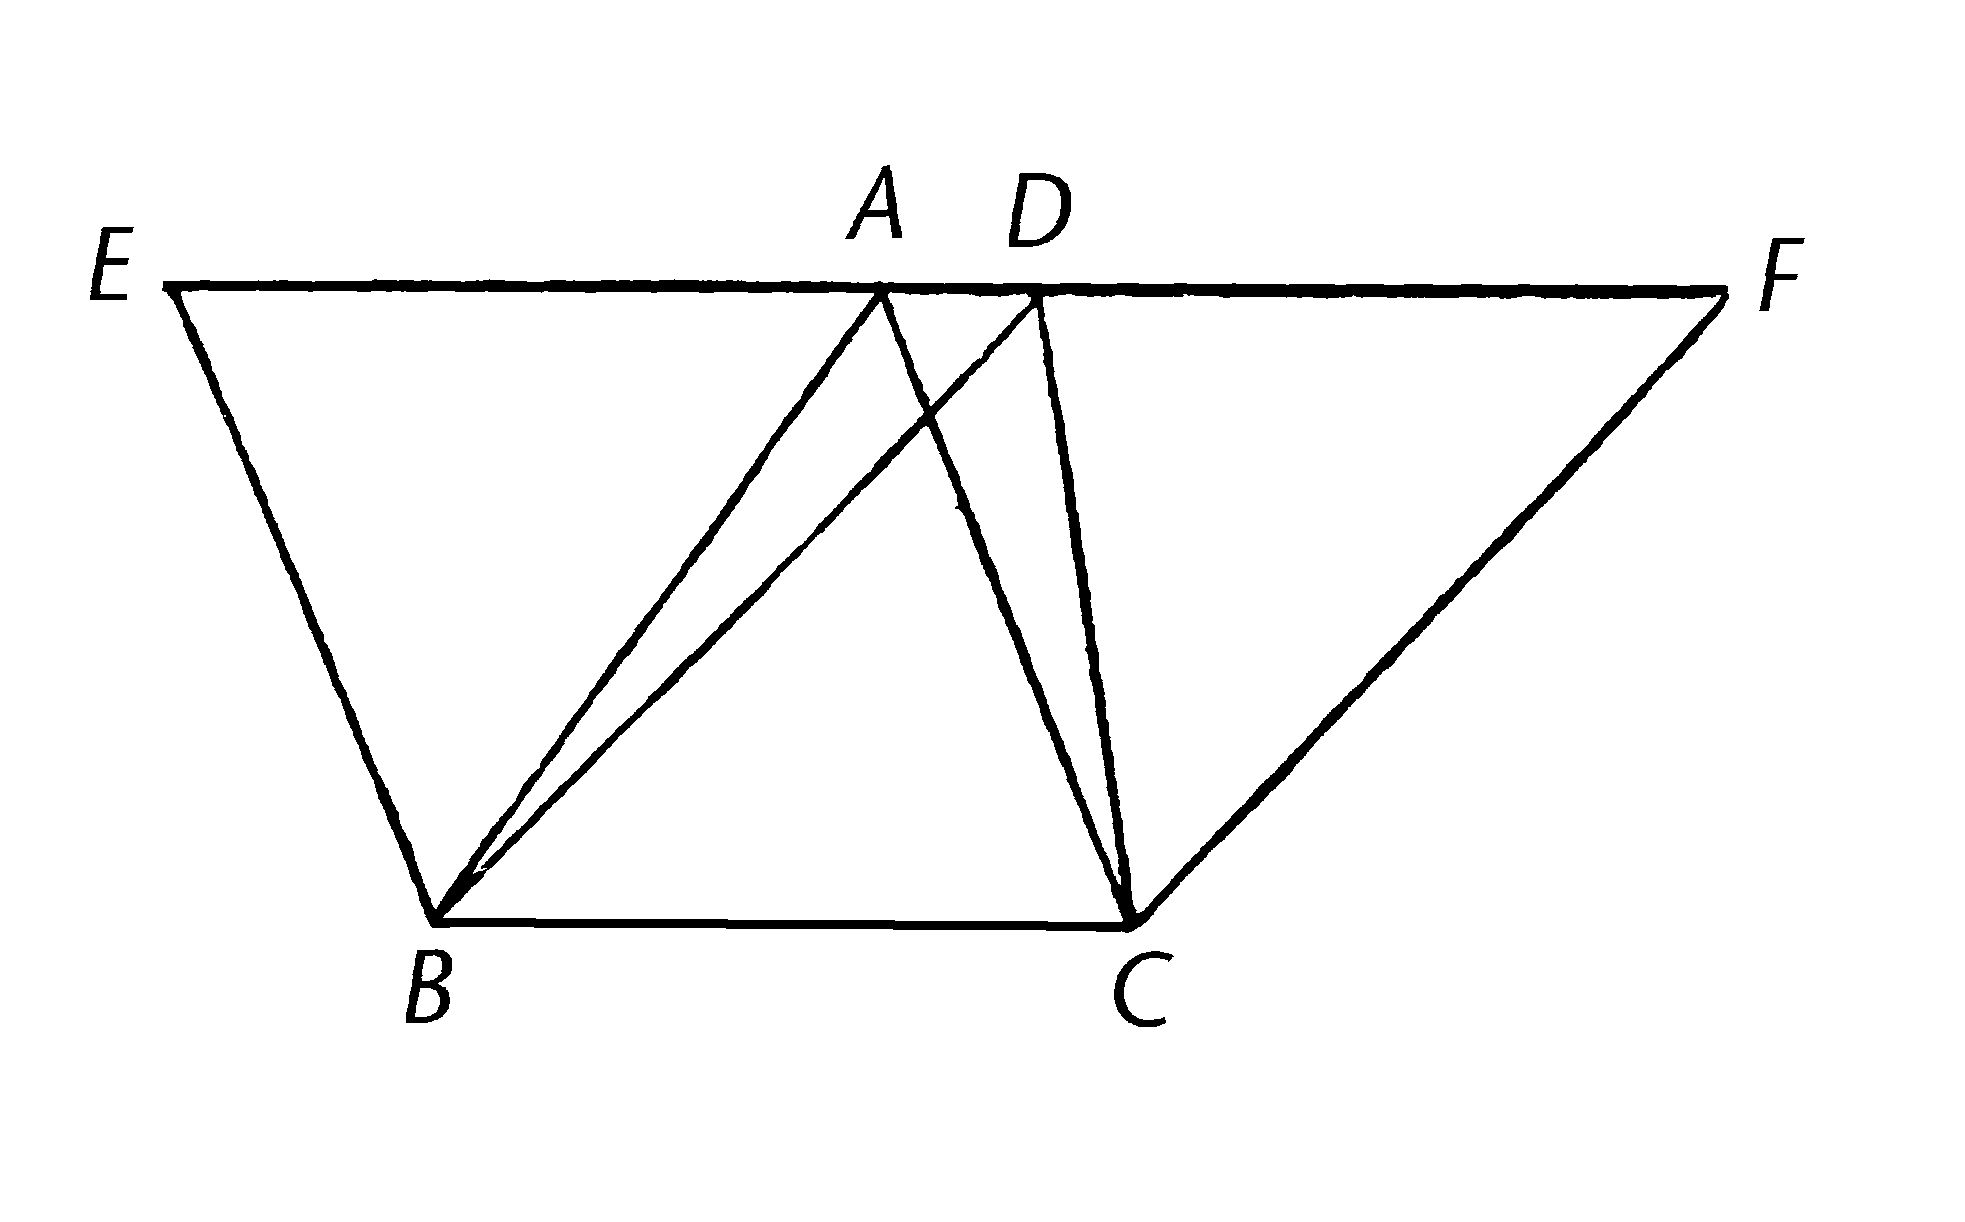
\includegraphics[width=0.5\linewidth]{./image/img532}

ABC,DBC是同底BC上的三角形,且在同平行线AD,BC之间;我说三角形ABC全等于三角形DBC。

向两个方向延长AD至E,F;过B画BE平行于CA【I.31】,且过C画CF平行于BD。【I.31】

那么图形EBCA,DBCF均为平行四边形;且它们相等,因为它们在同底BC上且在同平行线BC,EF间。【I.35】

此外,三角形ABC是平行四边形EBCA的一半;因为对角线AB将之平分。【I.34】

三角形DBC是平行四边形DBCF的一半;因为对角线DC将之平分。【I.34】

「但是相等事物的一半也互等。」

所以三角形ABC全等于三角形DBC。

综上所述\ldots\ldots{}

Q.E.D.

问题示例:

\begin{itemize}
\tightlist
\item
  现在我们发现我们可以对三角形的不同形状做同样的拓展。为什么欧几里得首先处理平行四边形?所有的事物,我们都是用三角形建造的,难道从三角形开始不会更简单一点么?
\item
  部分早期的编辑曾经在这儿加了一个公设并且填写了一个引用(文中的「」)。但是欧几里得似乎并不认为需要标注每一个涉及常理的推导元素。他是以同样的方式作的公理和定义么,只给我们基本的概念?公理会不会列出例子(最基本的或最重要的)来让我们理解用于推导的原理,识别我们大脑推导的方式?这里的主意是让我们有足够的例子,然后领会公理这一类别么?**
\item
  对于一半的例子,额外的解释性公理是不是多余?事实上,你能用归谬法证明它么?
\end{itemize}

\hypertarget{ux547dux9898ux4e09ux5341ux516b}{%
\section{命题三十八}\label{ux547dux9898ux4e09ux5341ux516b}}

\textbf{等底且在同组平行线之间的三角形互等。}

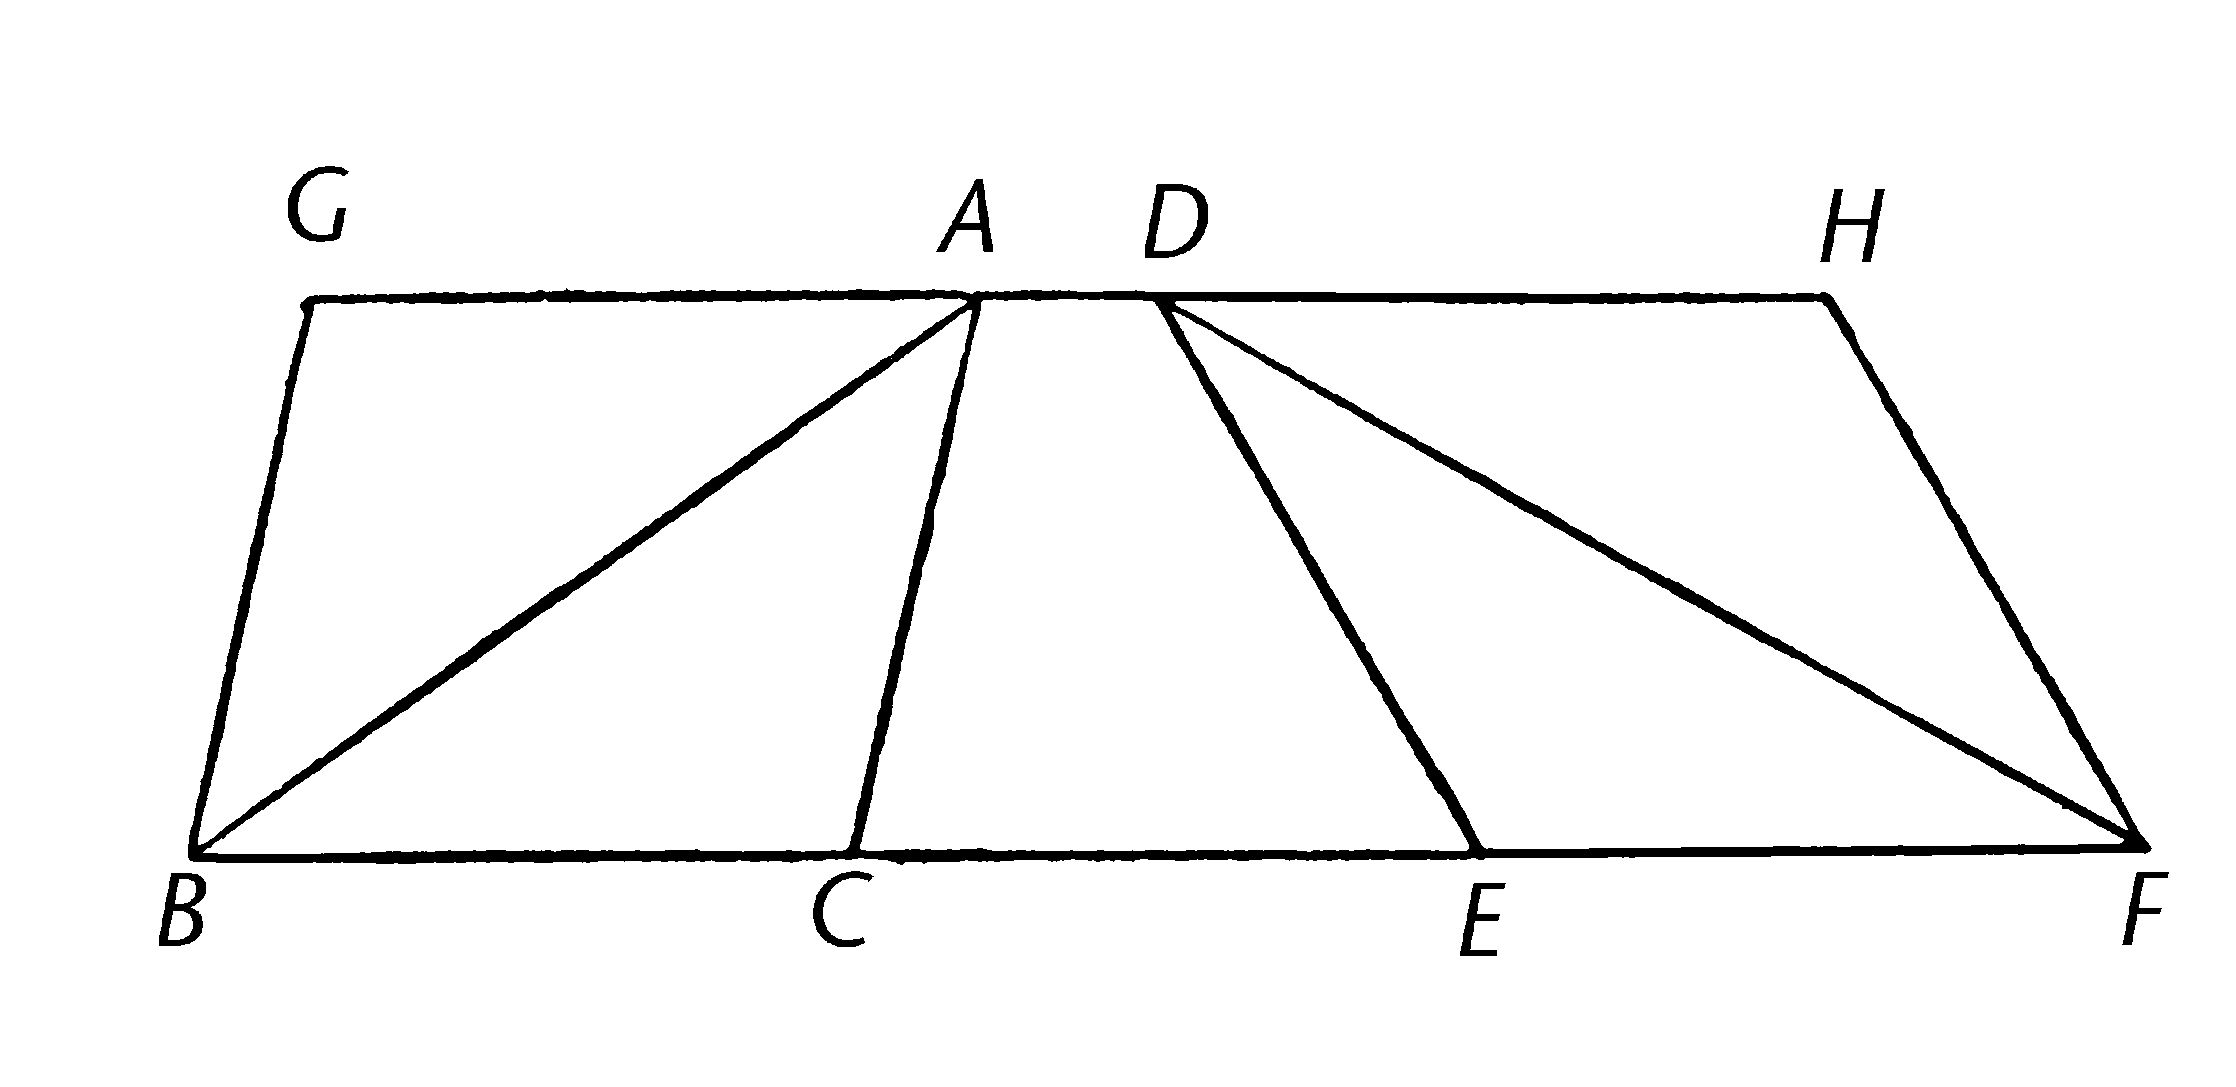
\includegraphics[width=0.5\linewidth]{./image/img534}

ABC,DEF是等底BC,EF上的三角形,且在平行线BF,AD之间;我说三角形ABC全等于三角形DEF。

向两个方向延长AD至E,F;过B画BG平行于CA【I.31】,且过F画FH平行于DE。

那么图形GBCA,DEFH均为平行四边形;且GBCA等于DEFH;因为它们在等底BC,EF上且在同平行线BE,GH之间。【I.36】

此外,三角形ABC是平行四边形GBCA的一半;因为对角线AB将之平分。【I.34】

三角形FED是平行四边形DEFH的一半;因为对角线DF将之平分。【I.34】

「但是相等事物的一半也互等。」

所以三角形ABC全等于三角形DEF。

综上所述\ldots\ldots{}

Q.E.D.

\hypertarget{ux547dux9898ux4e09ux5341ux4e5d}{%
\section{命题三十九}\label{ux547dux9898ux4e09ux5341ux4e5d}}

\textbf{同底的同侧全等三角形在同组平行线之间。}

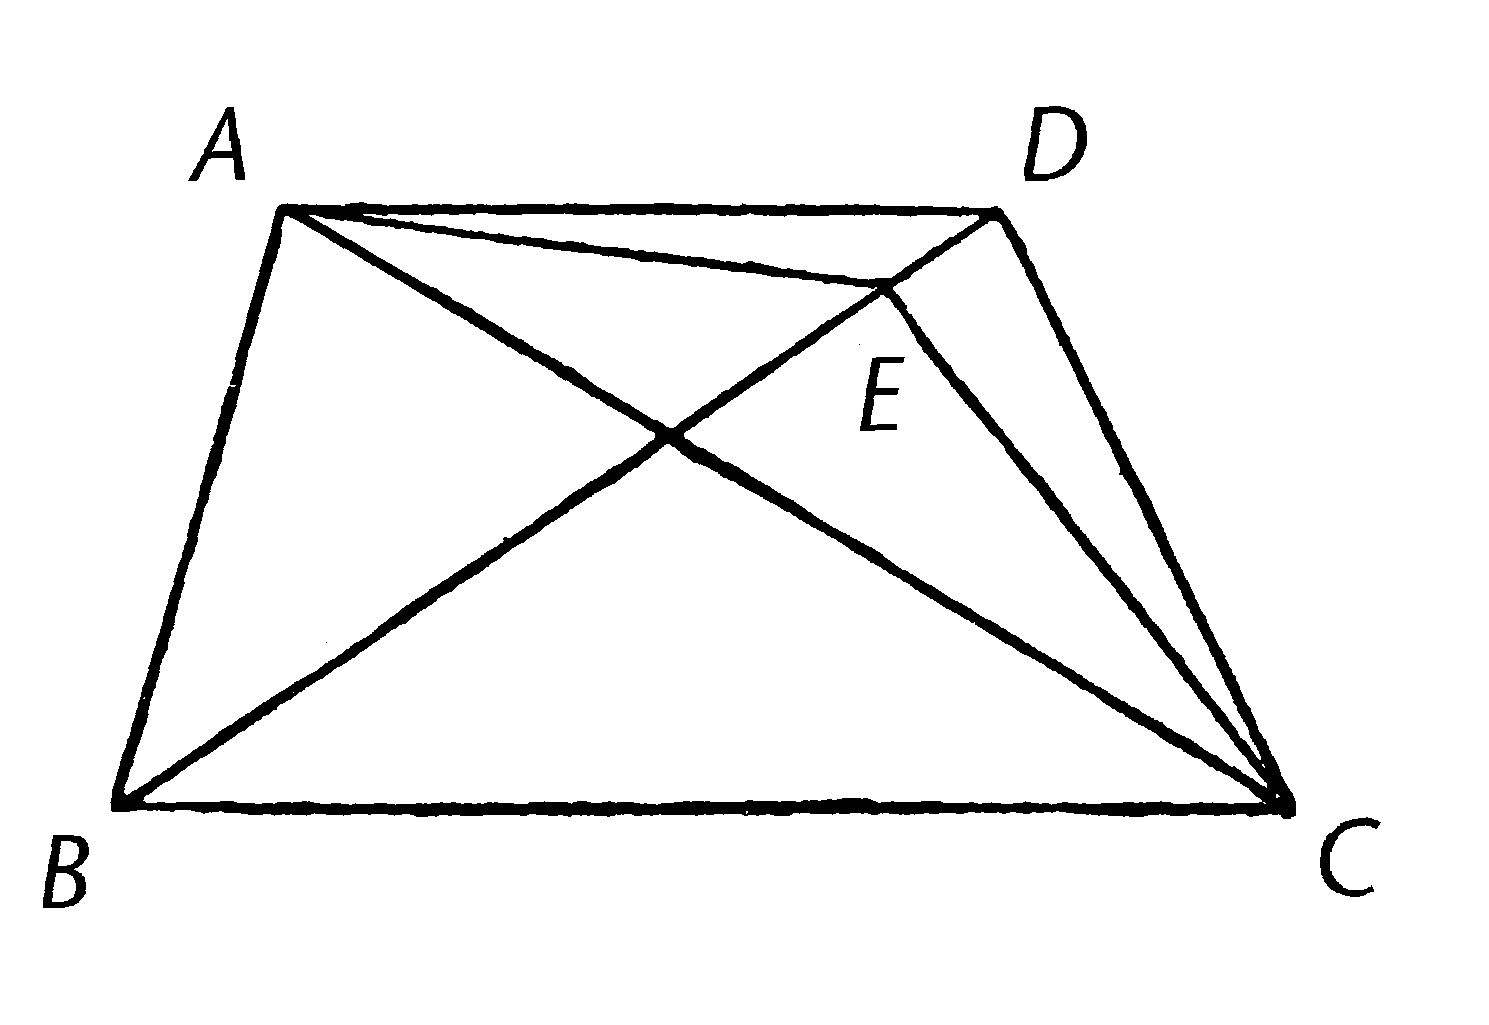
\includegraphics[width=0.4\linewidth]{./image/img536}

ABC,DBC是在同底BC同一侧上的全等三角形;「我说它们也在同平行线之间。」

连接AD;我说AD平行于BC。

因为如果不的话,过点A画AE平行于直线BC【I.31】,且连接EC。所以三角形ABC全等于三角形EBC;因为它们在同底BC上且在同平行线之间。【I.37】

但是ABC全等于DBC;所以DBC也全等于EBC【公理1】,大的等于小的:这是不可能的。

所以AE不平行于BC。

类似地,我们可以证明除AD外没有其它直线平行;所以AD平行于BC。

综上所述\ldots\ldots{}

Q.E.D.

\hypertarget{ux547dux9898ux56dbux5341}{%
\section{「命题四十」*}\label{ux547dux9898ux56dbux5341}}

\textbf{等底的同侧全等三角形在同组平行线之间。}

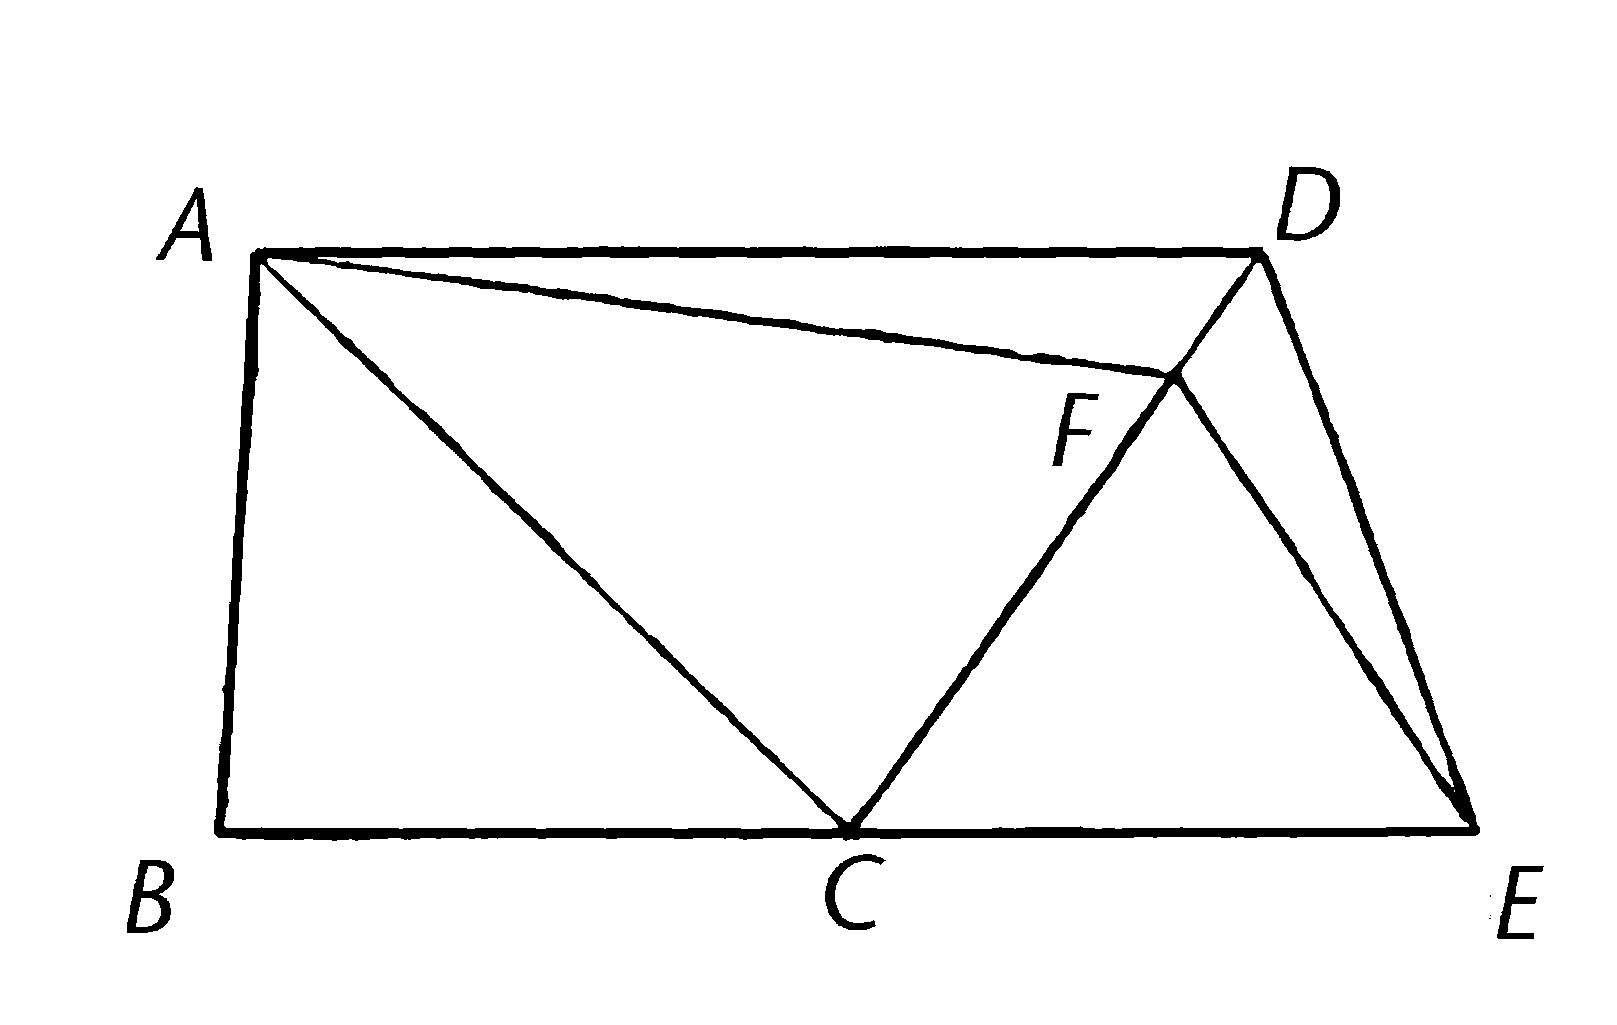
\includegraphics[width=0.4\linewidth]{./image/img538}

ABC,CDE是等底BC,CE同一侧上的全等三角形。我说它们也在同平行线之间。

连接AD;我说AD平行于BE。

如果不是的话,过A画AF平行于BE【I.31】,并连接FE。

所以三角形ABC等于三角形FCE;因为它们在同底BC,CE上且在同平行线BE,AF之间【I.38】。

但是三角形ABC全等于三角形DCE;所以三角形DCE也全等于三角形FCE【公理1】,大于等于小的:这是不可能的。所以AF不平行于BE。

类似地,我们可以证明除AD外没有其它直线平行;所以AD平行于BE。

综上所述\ldots\ldots{}

Q.E.D.

**编者注:整个命题I.40被「」是因为,根据Health的说法,``Heiberg曾证明\ldots 这个命题是补写的'',被一个未知的编辑。

\hypertarget{ux547dux9898ux56dbux5341ux4e00}{%
\section{命题四十一}\label{ux547dux9898ux56dbux5341ux4e00}}

\textbf{如果一个平行四边形和一个三角形共底且在同组平行线之间,那么此平行四边形是三角形的两倍。}

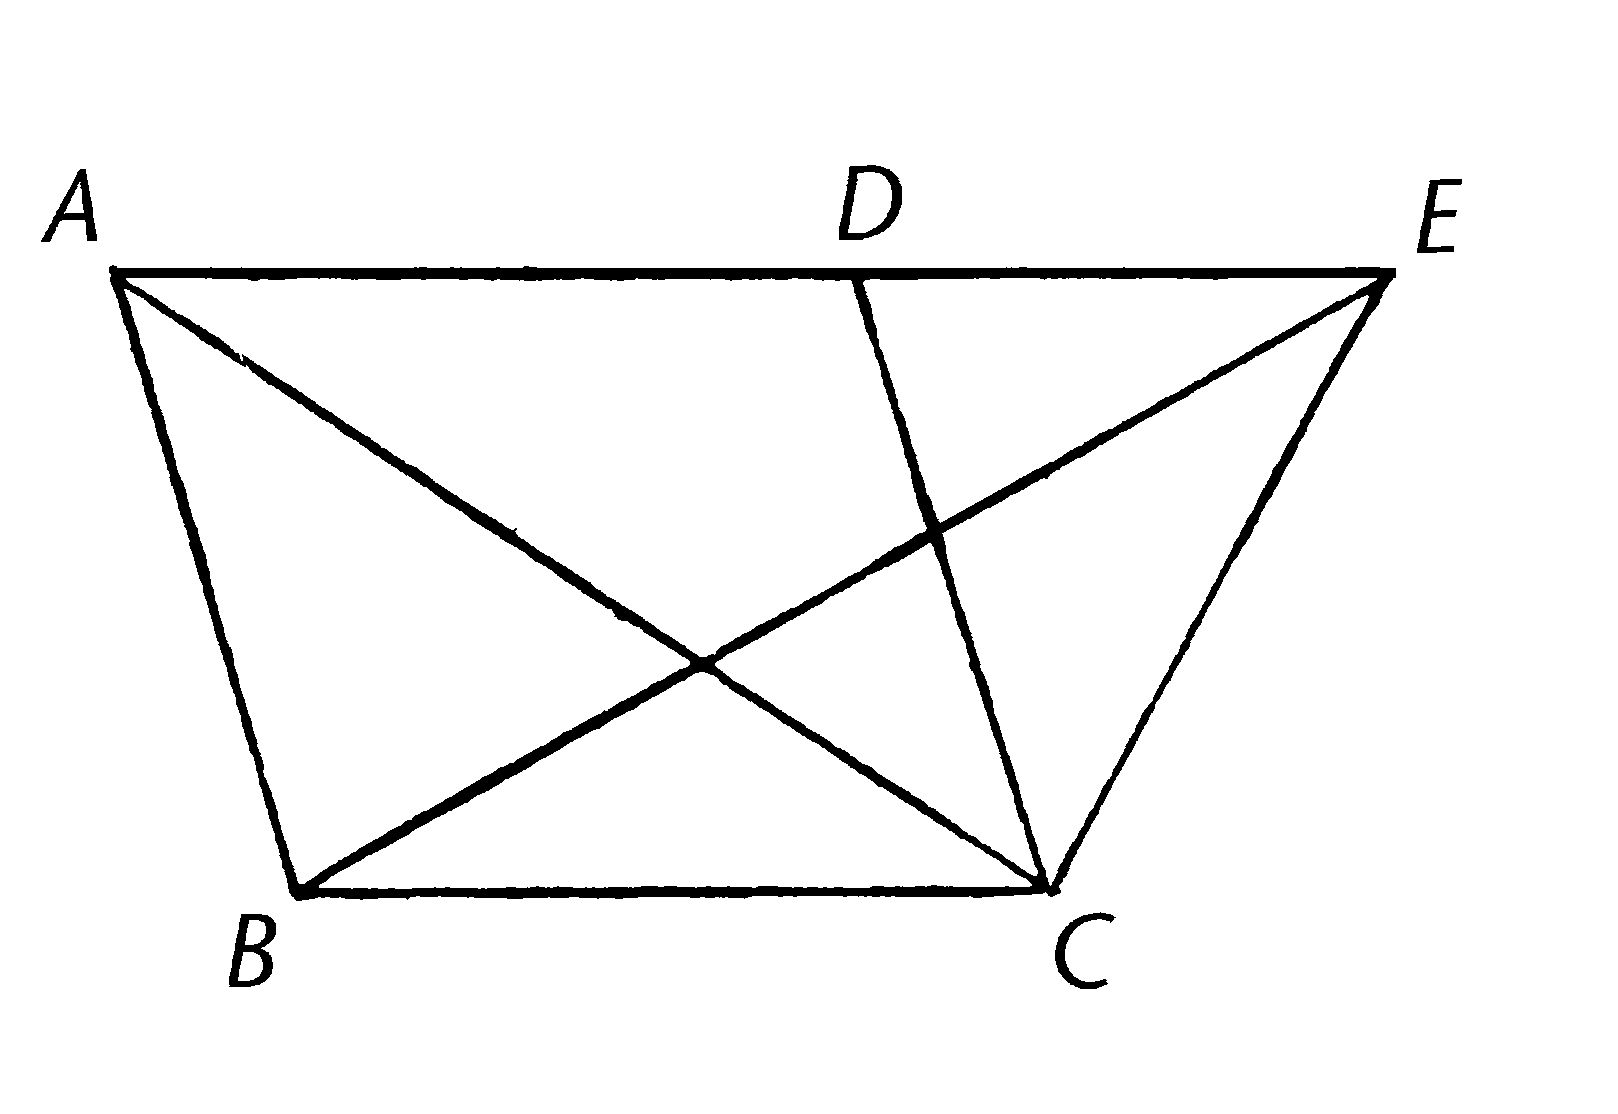
\includegraphics[width=0.4\linewidth]{./image/img540}

平行四边形ABCD和三角形EBC在同底BC上,且在同平行线BC,AE之间;

我说平行四边形ABCD是三角形BEC的两倍。

连接AC。

那么三角形ABC全等于三角形EBC;因为它们在同底BC上且在同平行线BC,AE之间。【I.37】

但是平行四边形ABCD是三角形ABC的两倍;因为对角线AC平分它【I.34】;所以平行四边形ABCD也是三角形EBC的两倍。

综上所述\ldots\ldots{}

Q.E.D.

问题示例:

\begin{itemize}
\tightlist
\item
  我们有没有留意到这个命题比较了不同图形的面积?(平行四边形的面积和三角形的面积) 我们可能没有留意,因为这个轻松的证明,还有在命题I.34中我们已经有了一个关于三角形和平行四边形隐含比较,也就是当我们看到对角线可以平分平行四边形成两个三角形时。但是这个看起来不会招致反对的步骤是我们到达I.45时,大胆而宽广地对不同图形面积等价的引领。
\end{itemize}

\hypertarget{ux547dux9898ux56dbux5341ux4e8c}{%
\section{命题四十二}\label{ux547dux9898ux56dbux5341ux4e8c}}

\textbf{用一个给定的直线角构建一个平行四边形,使之等于给定的三角形。}

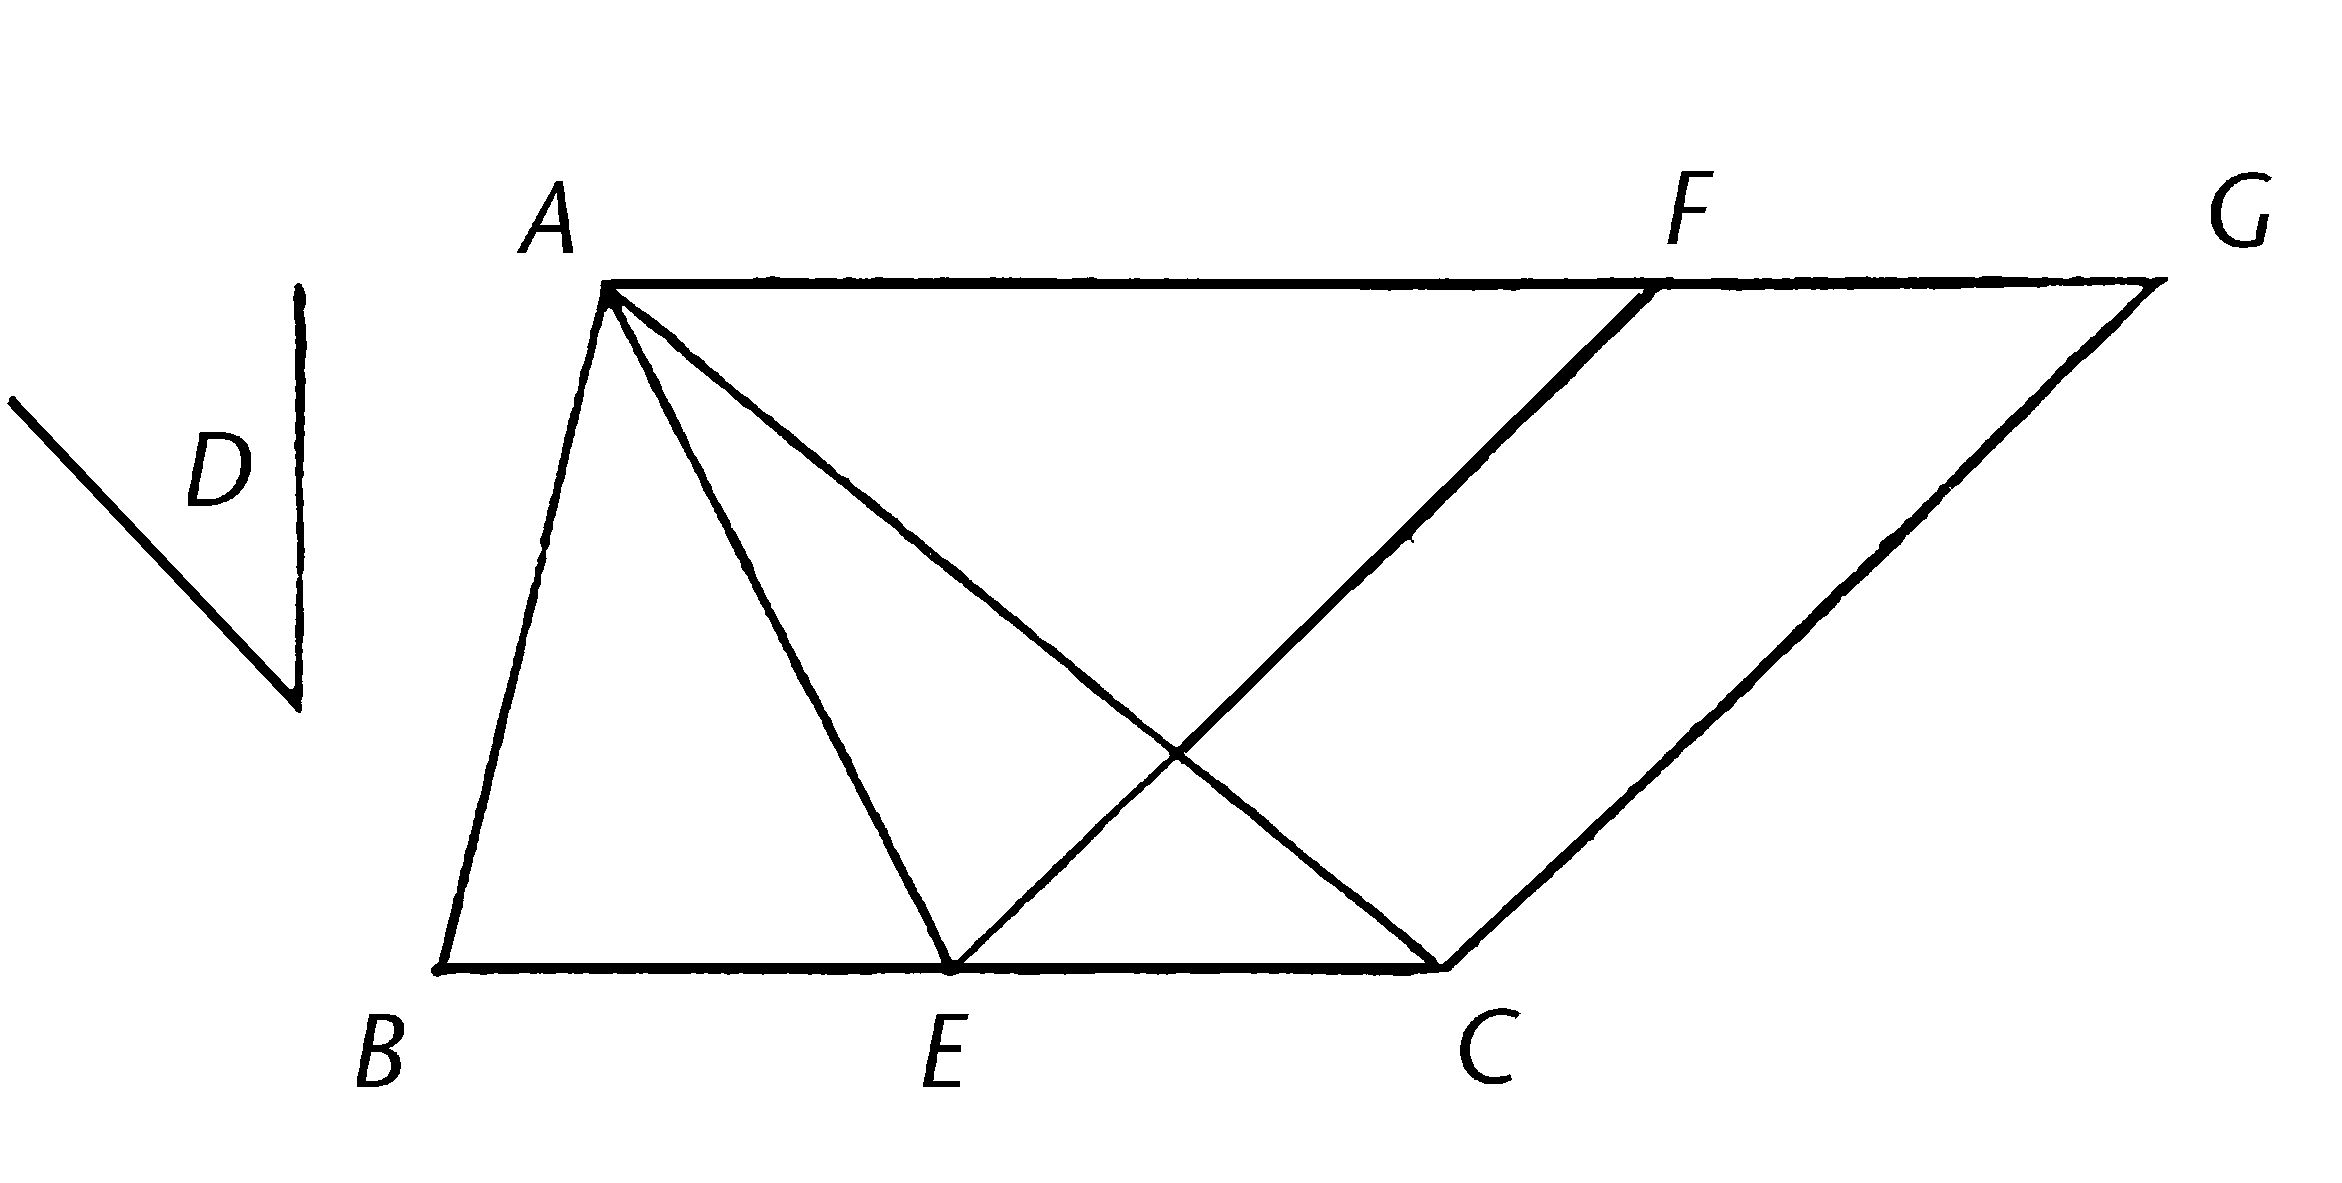
\includegraphics[width=0.5\linewidth]{./image/img542}

ABC是给定三角形,D是给定直线角,那么需要在直线角D上构建平行四边形,使与三角形ABC相等。

平分BC在E,连接AE;在直线EC的点E上,构建等于角D的角CEF【I.23】;过A画AG平行于EC, 过C画CG平行于EF【I.31】。

那么FECG是平行四边形。

又因为BE等于EC,三角形ABE也全等于三角形AEC,因为它们在等边BE,EC且在同平行线BC,AG之间【I.38】;所以三角形ABC使三角形AEC的两倍。

但是平行四边形FECG也是三角形AEC的两倍,因为它们在同底上且在同平行线之间;所以平行四边形FECG等于三角形ABC。

且其中角CEF等于给定角D。

所以构建的平行四边形FECG与给定三角形ABC相等,在与角D相等的角CEF上。

Q.E.F.

问题示例:

\begin{itemize}
\tightlist
\item
  在前一个命题中,我们几乎可以从图像中一眼看到证明。这儿就不能一眼到底了,因为角D不在边上。尽管用我们已经放入工具箱的命题已足以使论证前行,但是注意!在简单应用之前结论的表面下,面积的转换,也就是我们对于面积相等性含义的认知也在发生变化。
\end{itemize}

\hypertarget{ux547dux9898ux56dbux5341ux4e09}{%
\section{命题四十三}\label{ux547dux9898ux56dbux5341ux4e09}}

\textbf{在任意一个平行四边形中,关于对角线的补形互等。}

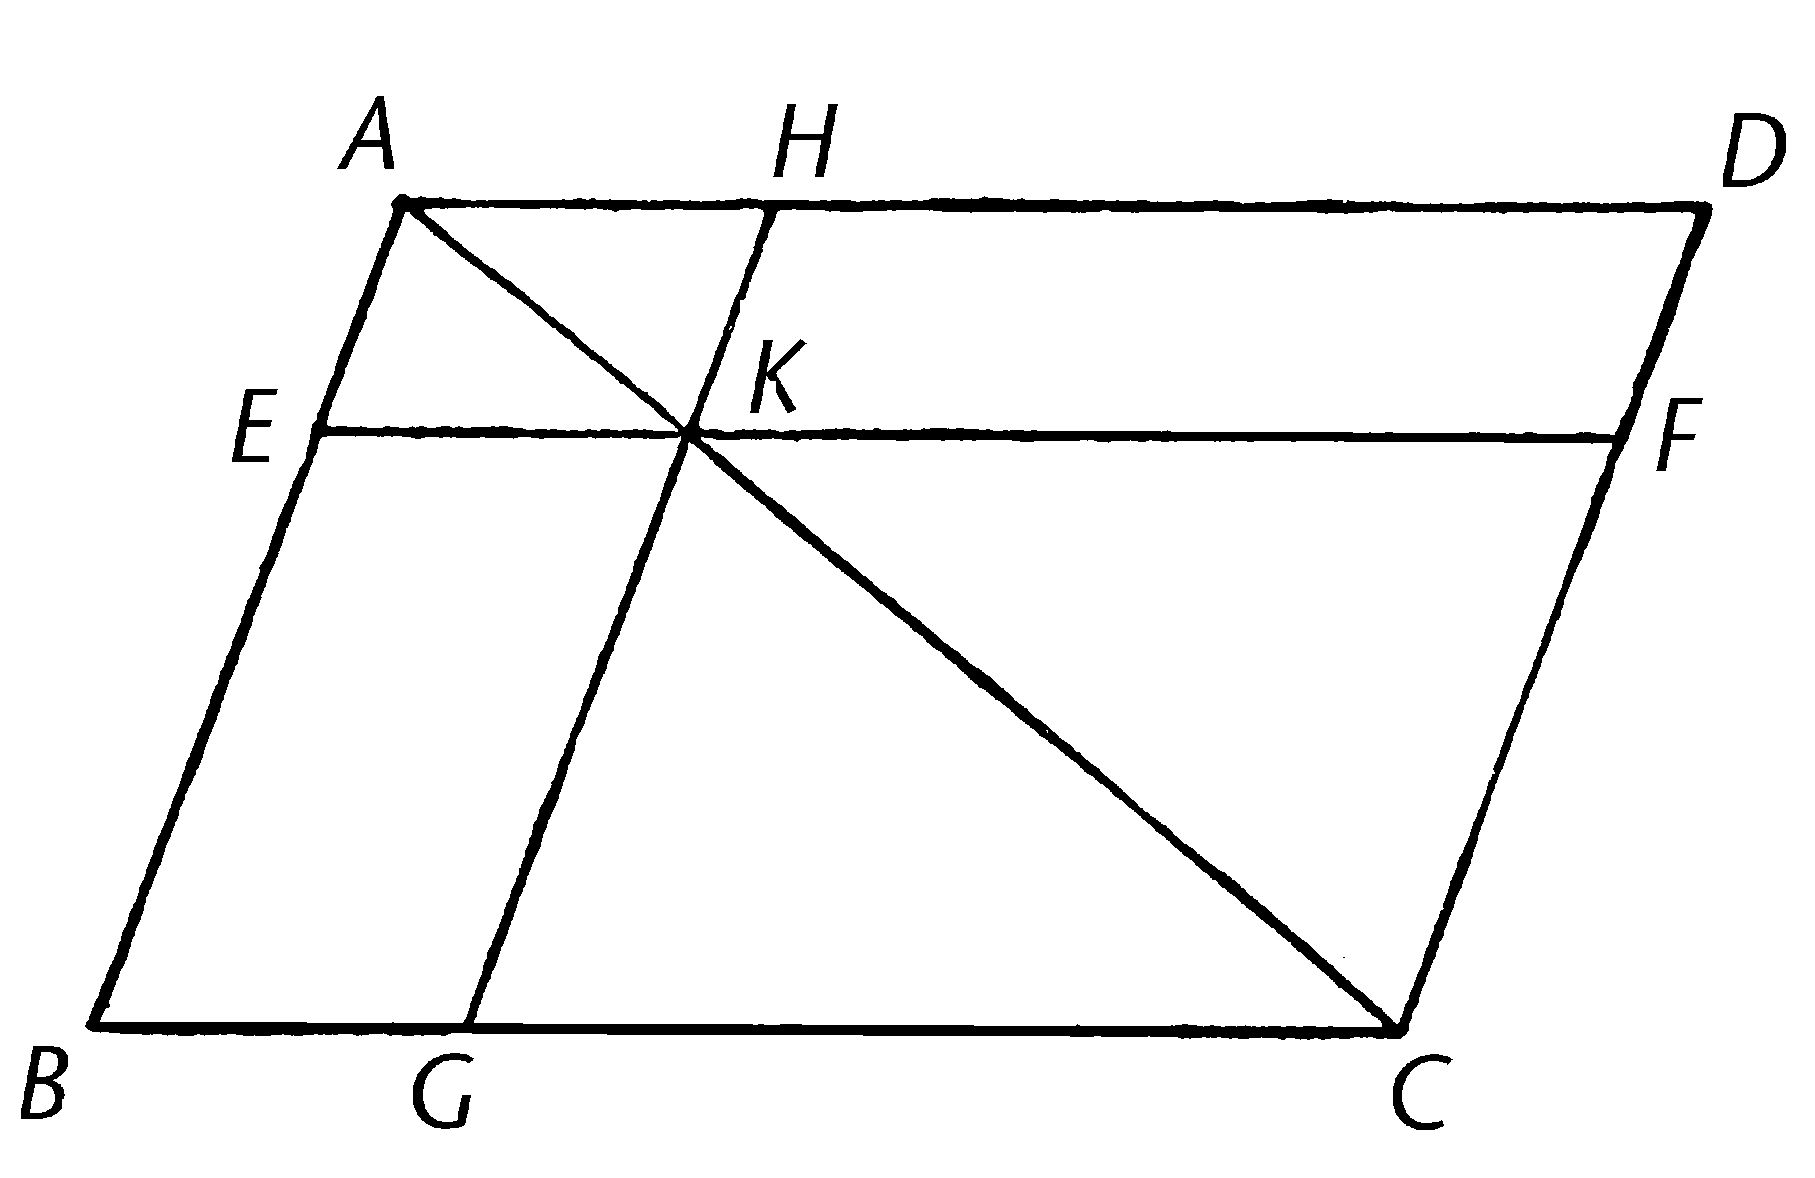
\includegraphics[width=0.3\linewidth]{./image/img544}

ABCD是平行四边形,且AC是它的对角线;在AC上作平行四边形EH,FG,CK,KD是所谓的补形;我说补形BK等于补形KD。

因为ABCD是平行四边形,且AC是其对角线,三角形ABC全等于三角形ACD。【I.34】

再一次,因为EH是平行四边形,且AK是其对角线,三角形AEK全等于三角形AHK。

同理可得,三角形KFC全等于三角形KGC。

现在,因为三角形AEK全等于三角形AHK, 且KFC全等于KGC,三角形AEK和KGC合在一起等于三角形AHK和KFC合在一起。【公理2】

且整个三角形ABC也等于整个ADC;那么剩余的补形BK也等于剩余的补形KD。

综上所述\ldots\ldots{}

Q.E.D.

***编者注:如果,在一个平行四边形中,围绕同一个对角线,还构造了其它的平行四边形,补形是剩余的空间。尽管这些补形的相等性可以在一系列可能的图形的加以证明,这儿及以后,欧几里得关心的是特殊的情况,也就是当围绕对角线的平行四边形有一个共同点K时的情况。这里的``补形''是被剩余空间所塑造的平行四边形,也就是BK和KD。

\hypertarget{ux547dux9898ux56dbux5341ux56db}{%
\section{命题四十四}\label{ux547dux9898ux56dbux5341ux56db}}

\textbf{用给定的线段和直线角作平行四边形,使等于给定的三角形。}

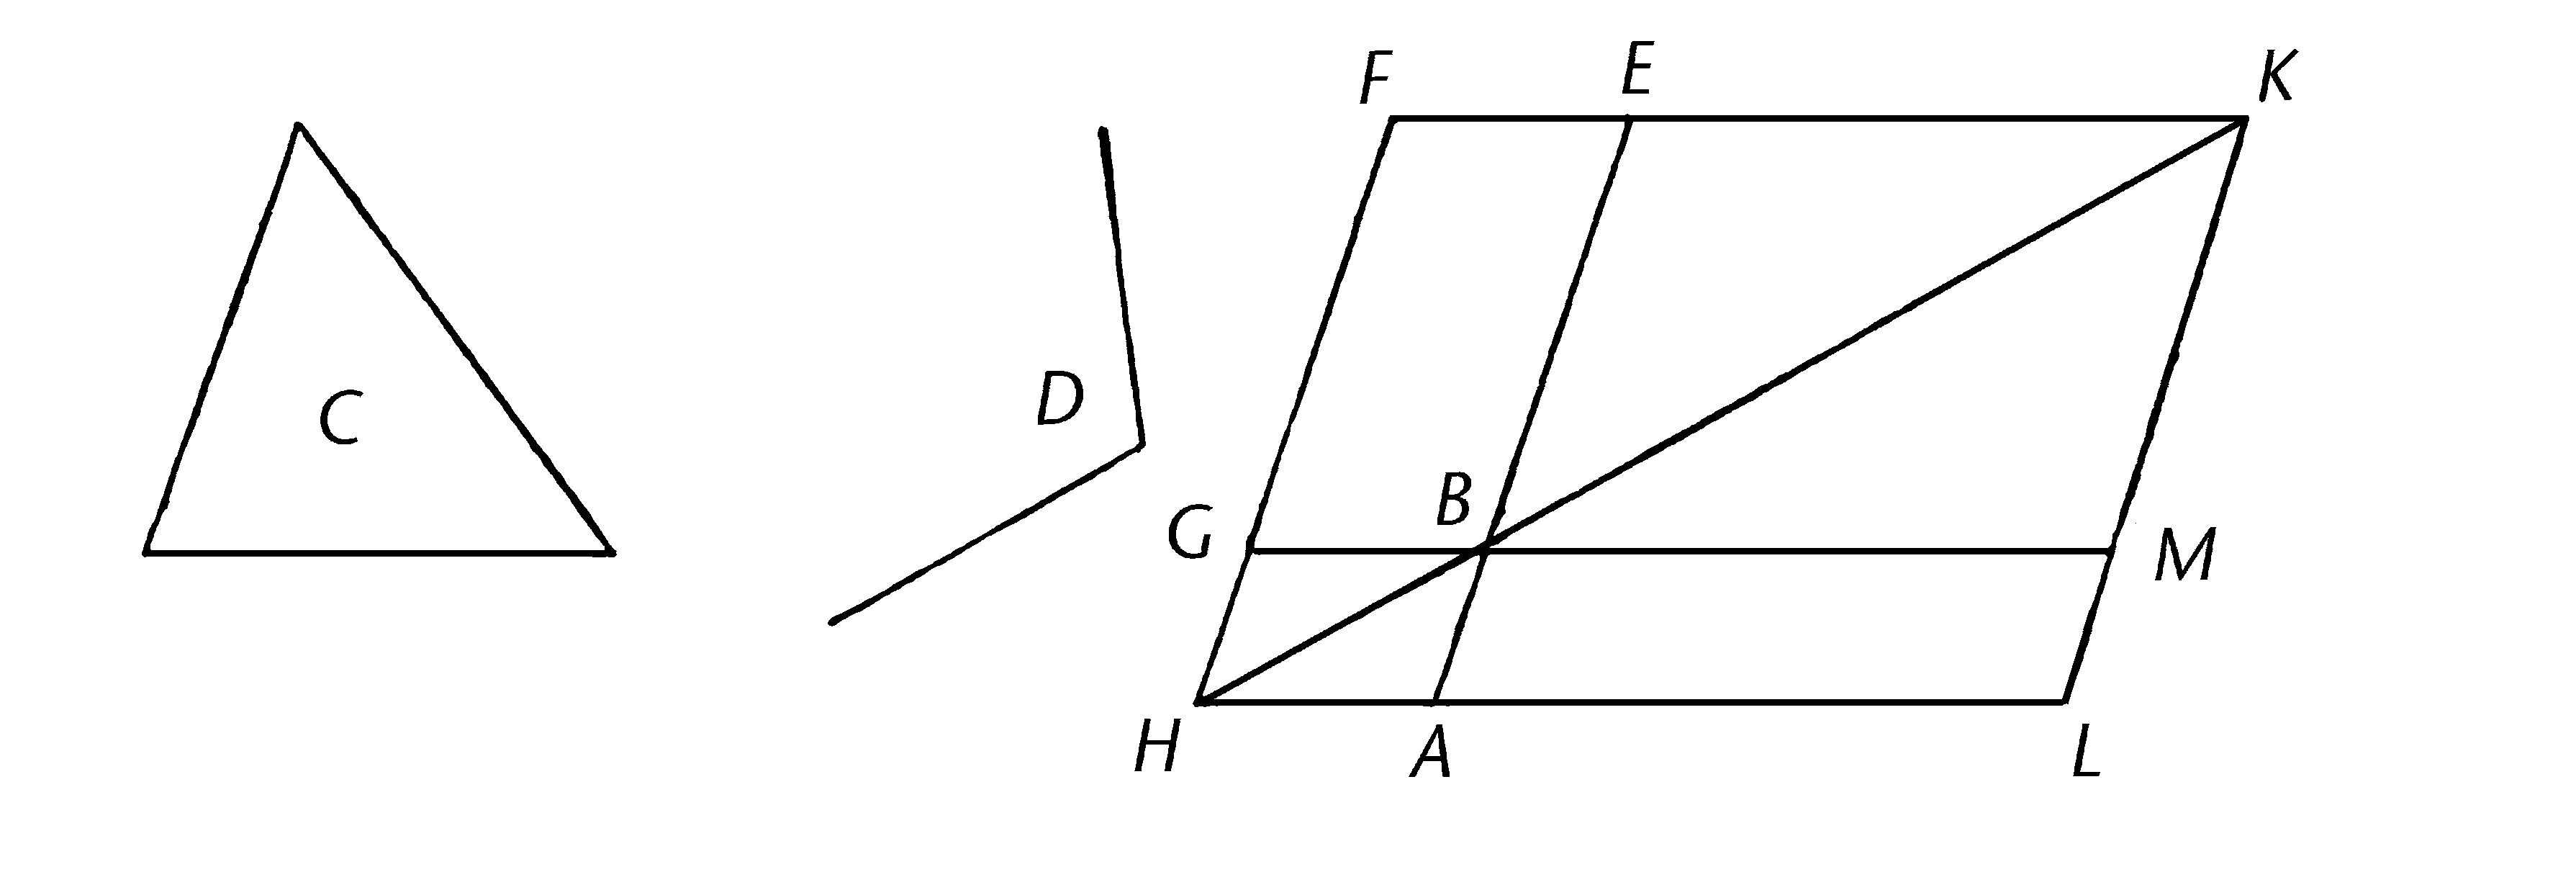
\includegraphics[width=0.5\linewidth]{./image/img546}

AB为给定直线,C为给定三角形,且D是给定直线角;那么需要在给定直线AB上,用与角D相等的角,应用一个平行四边形,使等于给定三角形C。

在等于角D的角EBG上构建平行四边形BEFG,使等于三角形C【I.42】;放置BE在与AB的同条直线上;画FG到H,且过A画AH平行于BG或EF。【I.31】

连接HB。

那么,因为直线HF落在平行AH,EF,角AHF,HFE等于两直角【I.29】。

那么角BHG,GFE小于两直角;且无限延长的直线在角小于两直角的一侧相交【公设5】;所以延长HB,FE会相交。

延长它们并在K相交;过点K,画KL平行于EA或FH,【I.31】且延长HA,GB到点L,M。

那么HLKF是一个平行四边形,HK是它的对角线,且AG,ME是平行四边形,且LB,BF是HK上所谓的补形;所以LB等于BF。【I.43】

但是BF等于三角形C;所以LB也等于C。【公理1】

又因为角GBE等于角ABM,【I.15】而角GBE等于角D,角ABM也等于角D。

所以等于给定三角形C的平行四边形LB在给定直线AB上,且角ABM与角D相等。

Q.E.F.

问题示例:

\begin{itemize}
\tightlist
\item
  欧耶!现在,不仅仅是在给定角上作给定的三角形,还要在给定的直线上!你有开始理所当然的认为欧几里得会用证明来完成它么?这是一个特别巧妙和漂亮的命题。Proclus,经典的欧几里得评论员,称呼这个方法为著名的``面积的应用''(applications of areas),古希腊数学所依赖的最有力方法之一。
\item
  你想要挑战么?在跟随欧几里得的证明之前,你能不能自己弄明白这个论证是如何前行的?(图像以及之前的命题都是你的线索。)
\item
  注意这个命题调用了公设5。公设5是如何成为证明的关键的?欧几里得在多少个命题里直接调用了这个公设?哪些命题间接的依赖它?
\end{itemize}

\hypertarget{ux547dux9898ux56dbux5341ux4e94}{%
\section{命题四十五}\label{ux547dux9898ux56dbux5341ux4e94}}

\textbf{用给定的直线角构建平行四边形,使等于给定的直线图形。}

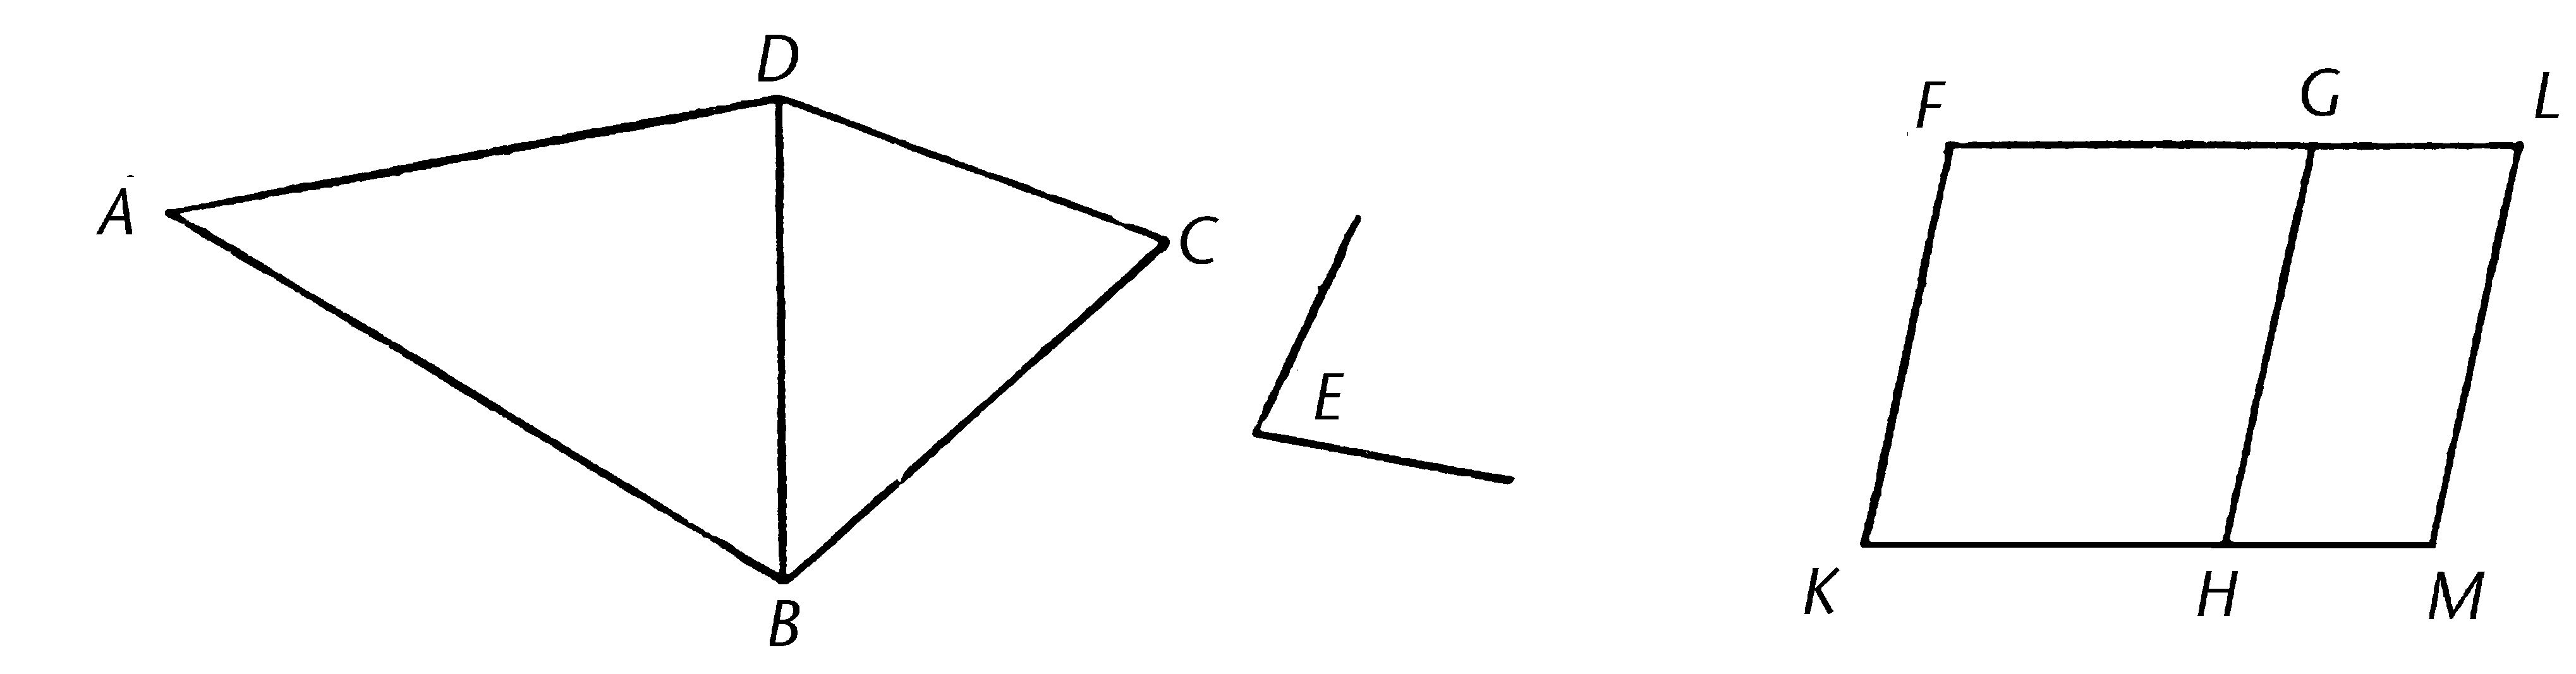
\includegraphics[width=0.5\linewidth]{./image/img549}

ABCD是给定的直线图形且E是给定的直线角;所以需要在给定角E上构建一个等于直线图形ABCD的平行四边形。

连接DB,且构建平行四边形FH并使其等于三角形ABD,其中角HKF等于角E【I.42】使与三角形DBC相等的平行四边形GM安置在直线GH上,其中角GHM等于角E。【I.44】

那么,因为角E 等于HKF,GHM任一,角HKF也等于角GHN。【公理1】

各自添加角KHG;所以角FKH,KHG等于角KHG,GHM。

但是角FKH,KHG等于两直角【I.29】;所以角KHG, GHM也等于两直角。

所以,在直线GH及点H上,未落在同侧的两直线KH,HM使得相邻角等于两直角;所以KH和HM在同一条直线上。【I.14】

又因为直线HG落在平行线KM,FG上,内错角MHG, HGF互等。【I.29】

各自添加角HGL;那么角MHG,HGL等于角HGF,HGL。【公理2】

但是角MHG,HGL等于两直角;所以角HGF,HGL也等于两直角。【公理1】

所以FG与GL在同一条直线上。【I.14】

又因为FK等于且平行于HG【I.34】,且HG与NL也是如此,KF等于且平行于ML【公理1; I。30】且直线KM,FL连接{[}它们的端点{]};所以KM,FL也相等且平行。【I.33】所以KFLM也是平行四边形。

又因为三角形ABD等于平行四边形FH,且DBC等于GM,整个直线图形ABCD等于整个平行四边形KFLM。

所以构建的平行四边形KFLM与给定的直线图形ABCD相等,其中角FKM等于给定角E。

Q.E.F.

问题示例:

\begin{itemize}
\tightlist
\item
  现在,我们用巧妙的命题44来构建一个平行四边形,在给定的角上,使等于``给定的直线图形''。也就是说,一个任意形状的四边形可以被转换成另一个四边形,不仅仅是任意其它一个,甚至可以是一个带有给定角的平行四边形。在早期命题的时候,你有想过这种事物存在的可能么?
\item
  为什么证明KH和HM,FG和GL落在同一条直线上是必需的?
\item
  这个命题可以被延伸到任意直线图形,不限制边数吗?你如何拓展这个证明以涵盖任意多边形?为什么欧几里得认为他只需要展示四边形?
\item
  这是个好的时机来回顾你脑海中的步骤,关于欧几里得引领你转换区域和转换关于区域相等性的想法。证明中步骤是有顺序的,这个顺序几乎可以被机械式地遵循。但是在同一时间,这里的想法也在演变。这两个过程之间的关系是什么?
\item
  也许有的人只是被动地过了一遍步骤,且在最后有一个能被使用的结果,它本身就像是步骤一样机械?在这种情况下失去了什么?会不会有人被告知了一种以某叙事方式考虑区域,但缺失逻辑论证的方法?也就是关于重合的概念如何被拓展到将该区域重排至另一种形状且两者始终相等?在这种情况下失去了什么?
\end{itemize}

\hypertarget{ux547dux9898ux56dbux5341ux516d}{%
\section{命题四十六}\label{ux547dux9898ux56dbux5341ux516d}}

\textbf{在给定的线段上作正方形。}

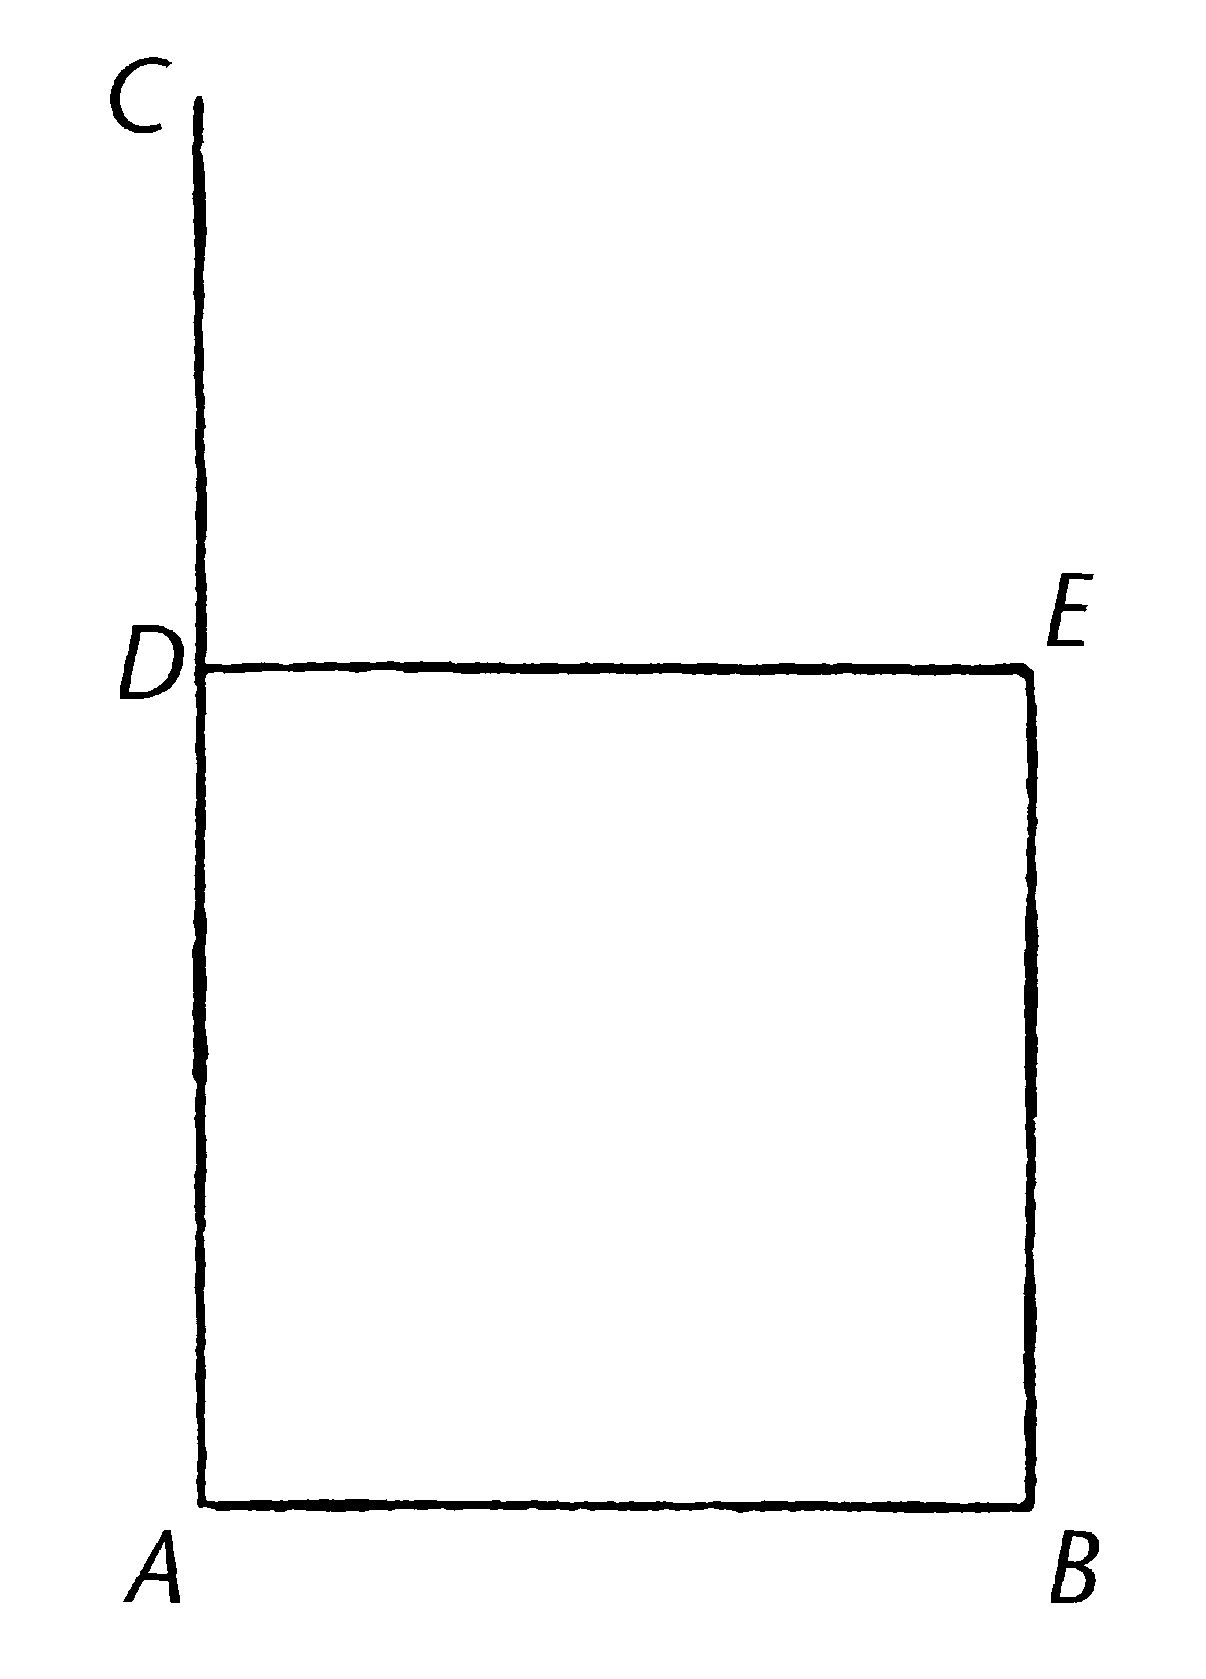
\includegraphics[width=0.2\linewidth]{./image/img552}

AB是给定的直线;那么需要在直线AB上画正方形。

从直线AB的A上画成直角的线AC,【I.11】且令AD等于AB;过点D作DE平行于AB, 过点B作BE平行于AD。【I.31】

那么ADEB是平行四边形;所以AB等于DE, AD等于BE。【I.34】

但是AB等于AD;那么四条直线BA,AD,DE,EB互等;那么平行四边形ADEB是等边的。

接下来,我说它也是全直角的。

因为直线AD落在平行线AB,DE上,角BAD,ADE等于两直角。【I.29】

但是角BAD是直的;所以角ADE也是直的。

且在平行四边形区域,对边及对角互等【I.34】;所以对角ABE,BED也是直的。

所以ADEB是全直角的。

且已证明是等边的。

所以它是一个正方形;且它在直线AB上。

Q.E.F.

问题示例:

\begin{itemize}
\tightlist
\item
  从第一个命题开始,我们就已经有构建还有论证。之前你有注意到构建都是有两部分的么?
\item
  比如说,这里的声明是说构建一个正方形;而且我们确实构建了一个正方形。我们是不是想过可以停在那儿了?为什么在那儿我们没有用Q.E.F.(``已成事实'')?为什么在Q.E.F.之前我们还要继续前行以证明它是一个正方形?这个会在脑海中提醒我们一系列的事情么,当我们作自己的证明时?
\item
  这里是不是有一个提示,只有在我们知道我们所做即所求的时候,关于想法的行动才算完成?我们需要知道我们建造了什么。欧几里得是不是在说``直到你理解你所做之前,你都没有完成我所要求的''?
\end{itemize}

\hypertarget{ux547dux9898ux56dbux5341ux4e03}{%
\section{命题四十七}\label{ux547dux9898ux56dbux5341ux4e03}}

\textbf{在直角三角形中,直角对边上的正方形等于夹直角的两边正方形之和。}

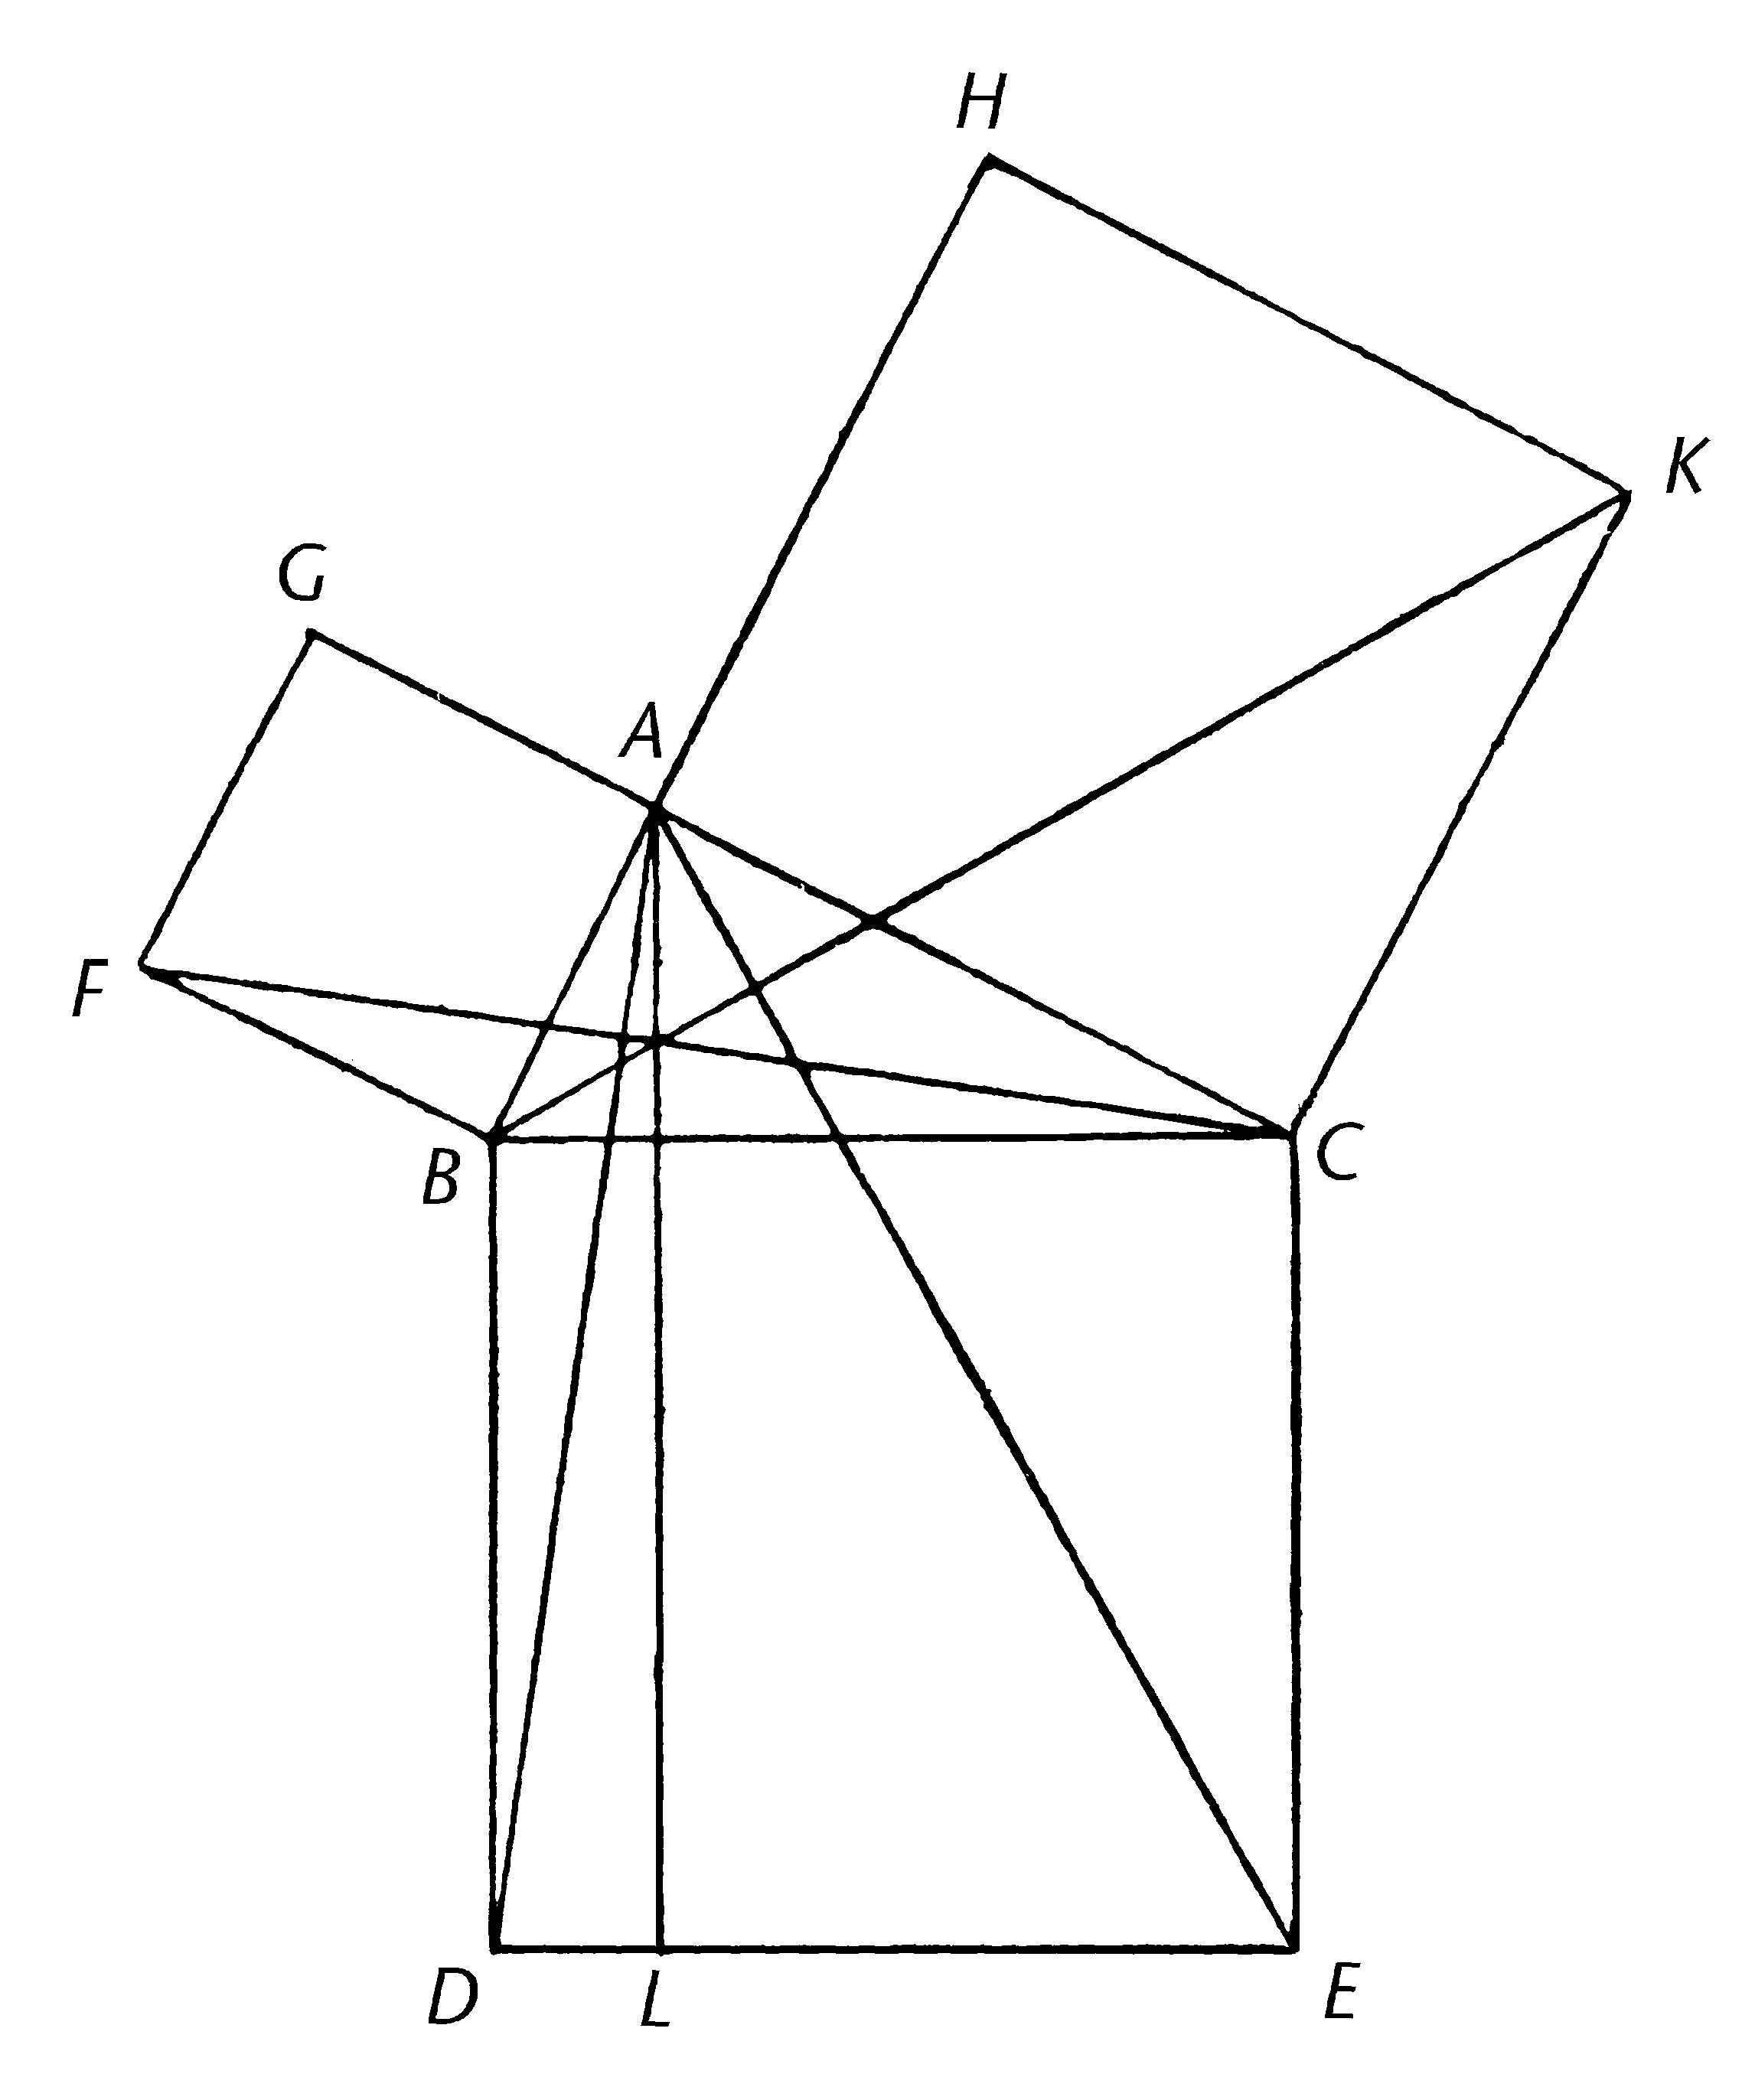
\includegraphics[width=0.3\linewidth]{./image/img555}

ABC是直角三角形且角BAC是直角;我说BC上的正方形等于BA,AC上的正方形们。

在BC上画正方形BDEC,在BA,AC上画正方形GB,HC【I.46】;过点A画AL平行于BD或CE,且连接AD,FC。
那么,因为BAC,BAG均为直角,随之在直线BA即点A上,未在同侧的两直线AC,AG使得相邻角等于两直角;那么CA与AG在同一条直线上【I.14】

同理可得,BA与AH在同一条直线上。

又因为角DBC等于角FBA;均为直角:各自添加角ABC;那么整个角DBA等于整个角FBC。【公理2】

又因为DB等于BC,FB等于BA,两边AB,BD与两边FB,BC互等;且角ABD等于角FBC;所以底边AD等于底边FC,三角形ABD等于三角形FBC。【I.4】

现在平行四边形BL是三角形ABD的两倍,因为它们在同底BD上,且在同平行线BD,AL之间【I.41】。

正方形GB是三角形FBC的两倍,因为它们在同底FB上,且在同平行线FB,GC之间【I.41】。

「但是相等事物的两倍也互等。」

所以平行四边形BL也等于正方形GB。

类似地,如果连接AE,BK,可证明平行四边形CL也等于正方形HC;所以整个正方形BDEC等于两个正方形GB,HC。【公理2】

且正方形BDEC画在BC上,正方形GB,HC在BA,AC上。

所以边BC上的正方形等于边BA,AC上的正方形们。

综上所述\ldots\ldots{}

Q.E.D.

问题示例:

\begin{itemize}
\tightlist
\item
  欧几里得证明正方形的边在直角三角形的边上,这个行为有没有提醒你,不能依赖于绘图显示的情况------它们看起来好像在一条直线上? 被图纸中这样的事物所误导是多么容易的一件事啊!除了这两条连续的直线是否真的在同一条直线上,还需要注意些什么?在绘图或者查看图像的时候,你如何确保足够小心以将此类事情记于心中?
\item
  I.47是关于正方形还是关于边的命题?还是另一种相等性?在这个命题之前,我们的理解是在相同的角度,区域。我们从叠合的区域到不同形状的区域。现在我们有线等于面积。我们有没有更进一步拓展了(用不同的方式)我们关于相等性的认知?
\item
  这个非常著名的命题,为Pythagoras(毕达哥拉斯)提供了一个关于三角形叠合的非常让人满意的应用,并且这个命题引申出了平行线之间三角形和四边形的关系。你是否有感觉到一个峰值,在卷一长期仔细的构建中?我们还有一个命题加入以结尾,但是这个精彩的命题是值得成为《几何原本》基石结尾的。
\end{itemize}

\hypertarget{ux547dux9898ux56dbux5341ux516b}{%
\section{命题四十八}\label{ux547dux9898ux56dbux5341ux516b}}

\textbf{如果在一个三角形中,一边上的正方形等于剩余两边上正方形之和,那么剩余两边所夹角为直角。}

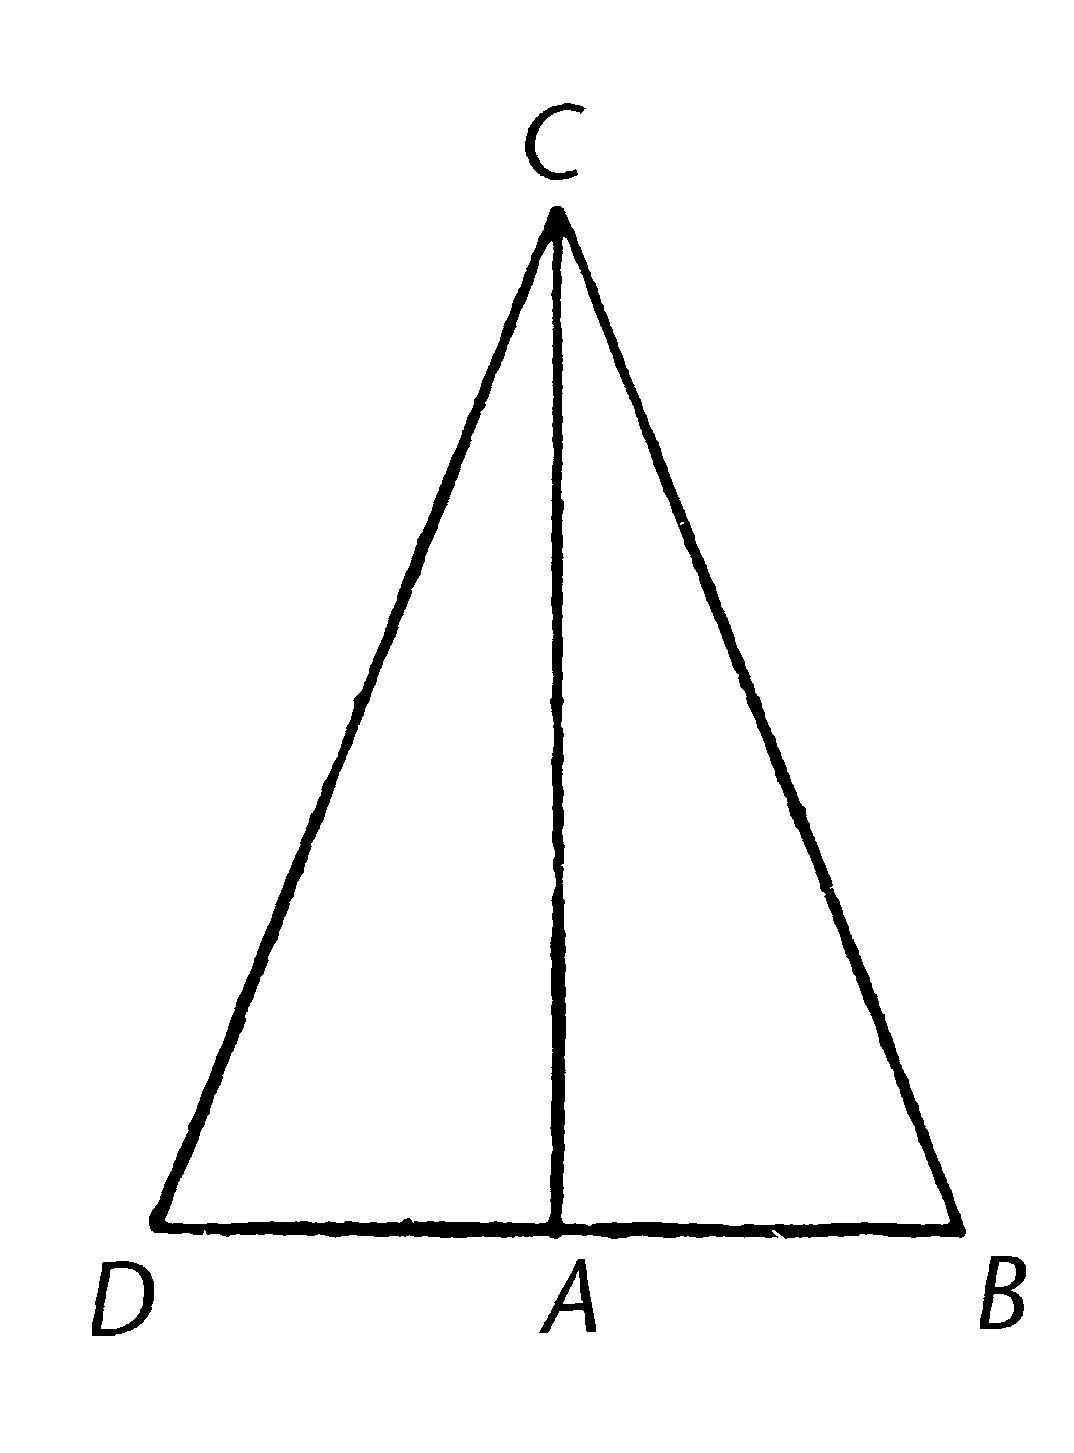
\includegraphics[width=0.2\linewidth]{./image/img558}

在三角形ABC中,是一边BC上的正方形等于边BA,AC上的正方形;我说角BAC是直的。

从直线AC的A上画成直角的线AD,使AD等于BA,连接DC。

因为DA等于AB,DA上的正方形也与AB上的正方形相等。

各自添加正方形AC;那么DA,AC上的正方形等于BA,AC上的正方形。

但是DC上的正方形等于DA,AC上的正方形,因为角DAC是直的【I.47】;BC上的正方形等于BA,AC上的正方形,因为这是我们的假设;所以DC上的正方形等于BC上的正方形,所以边DC等于BC。

又因为DA等于AB,且AC是共有的,两边DA,AC等于两边BA,AC;且边DC等于边BC;那么角DAC等于角BAC。【I.8】

但是角DAC是直的;那么角BAC也是直的。

综上所述\ldots\ldots{}

Q.E.D.

问题示例:

\begin{itemize}
\tightlist
\item
  我们需要证明I.47的逆命题么?是不是有些命题的逆命题需要被证明,而有些不用?还是说有些逆命题为真,有些为假,如果不证明这些逆命题的话你就不能确定?几何的逆命题和逻辑的逆命题是不一样的么?
\item
  卷一是什么形状的?像草?像一棵树?一棵有着另一棵从此树上长出来的树?还是像一只动物,比如说青蛙?还是像鸡蛋孵成了小鸡?到最后了,你如何描绘跟随的这个逻辑体系的特征?从最开始------点是没有部分的------而展开的。
\end{itemize}

\hypertarget{ux7ed3ux675fux8bed}{%
\section*{结束语}\label{ux7ed3ux675fux8bed}}
\addcontentsline{toc}{section}{结束语}

你喜欢这个么?你不希望它结束?这不是必须的!还有12卷书是一样的精彩!它们在一套完整的版本中;详细信息请参阅后文。想读更多的欧几里得?参考:

\begin{itemize}
\item
  Euclid's Elements: All Thirteen Books Complete in One Volume
\item
  The Bones: A handy, where-to-find-it pocket reference companion to Euclid's Elements
\end{itemize}

【宣棋注:以下两本书均为同一出版社的英文版,没有中文版,因此此处省略英文介绍的翻译。简单的介绍:第一本是欧几里得《几何原本》十三册全集,第二本是口袋书,只有各命题的声明和图,没有详细的证明。】

\hypertarget{ux7d22ux5f15ux53caux6c47ux7f16}{%
\chapter*{索引及汇编}\label{ux7d22ux5f15ux53caux6c47ux7f16}}
\addcontentsline{toc}{chapter}{索引及汇编}

宣棋注:此部分的原文是英文和古希腊语词汇对应表,是为了保持翻译的一惯性和流畅性。译者在此同时标注相应中文。在翻译过程中逐渐补充填充此表,不保证完成度,古希腊语由于字体的原因暂缺待补。

原文(英文词/希腊语词源/文本位置) 中文

\begin{itemize}
\tightlist
\item
  A

  \begin{itemize}
  \tightlist
  \item
    Adjacent (ejfexh`'' = in order), I. Def. 10 (p.~4) 相邻角
  \item
    Alternate (ejnallavx), of angles, I. 27 (p.~50)\\
  \item
    Angle

    \begin{itemize}
    \tightlist
    \item
      rectilineal, I. Def. 9 (p.~3) 直线角
    \item
      adjacent, I. Def. 10 (p.~4) 相邻角
    \item
      alternate, I. 27 (p.~50) 内错角
    \item
      exterior and interior (to a figure), I. 16 (p.~34)\\
    \item
      interior and opposite, I. 16 (p.~34) 内对角
    \item
      vertical, I. 15 (p.~33) 对顶角
    \end{itemize}
  \item
    Area (cwrivon), pp.~59-60 区域
  \end{itemize}
\item
  B

  \begin{itemize}
  \tightlist
  \item
    Base

    \begin{itemize}
    \tightlist
    \item
      of triangle, I. 4 (p.~16) 底边
    \end{itemize}
  \item
    Boundary (o\{ro\textasciitilde), I. Defs. 13, 14 (p.~4) 界限
  \end{itemize}
\item
  C

  \begin{itemize}
  \tightlist
  \item
    Circle, definition, I. Def. 15 (p.~5) 圆

    \begin{itemize}
    \tightlist
    \item
      circle (kuvklo\textasciitilde) and circumference (perifevreia) bisected by diameter, I. Def. 17 (p.~5) 圆和圆周
    \end{itemize}
  \item
    Compass and Straightedge, p.~10 圆规和直尺
  \item
    Complement, paraplhvroma, ``(figure) put in to fill up,'' I. 43 (p.~71) 补形
  \item
    Conclusion, sumpevrasma, necessary part of a proposition, pp.~xi, xii 结论
  \item
    Construction, kataskeuh,v one of the formal divisions of a proposition, pp.~xi, xii 构建
  \end{itemize}
\item
  D

  \begin{itemize}
  \tightlist
  \item
    Definition, in sense of ``closer statement'' (diorismov\textasciitilde), one of the formal divi- sions of a proposition, p.~xi 定义
  \item
    Diameter (diavmetro\textasciitilde), of circle or parallelogram, I. Def. 17 (p.~5) 直径
  \item
    Distance (diavsthma), in the sense of ``radius,'' I. Post. 3 (p.~7) 距离
  \item
    Divided Line, see Plato 柏拉图的分割线
  \item
    Drawing, see Compass and Straightedge 绘图
  \end{itemize}
\item
  E

  \begin{itemize}
  \tightlist
  \item
    Elements, definition, p.~xi 原本(元素)
  \item
    Enunciation (provtasi''), one of the formal divisions of a proposition, pp.~xi, xii 声明
  \item
    Equality, in sense different from that of congruence, I. 35 (p.~61). 相等
  \item
    Equilateral triangle, defined, I. Def. 20 (p.~6) constructed, I. 1 (p.~13) 等边三角形
  \item
    Euclid, about, p.~ix 欧几里得
  \item
    Exterior and interior (of angles), I. 16 (p.~34)\\
  \item
    Extremity, pevra\textasciitilde, I. Defs. 3, 13 (pp.~3, 4) 极端(端点)
  \end{itemize}
\item
  F

  \begin{itemize}
  \tightlist
  \item
    Figure (sch`ma), I. Def. 14, (p.~4) 图形
  \end{itemize}
\item
  G

  \begin{itemize}
  \tightlist
  \item
    Guidance for Study of the Propositions, pp.~11--12 学习命题的指引
  \end{itemize}
\item
  I

  \begin{itemize}
  \tightlist
  \item
    Isosceles (ijsoskelhv'') triangle, defined, I. Def. 20 (p.~6) 等腰三角形
  \end{itemize}
\item
  L

  \begin{itemize}
  \tightlist
  \item
    Line, straight (eujqei`a), I. Def. 4 (p.~3) 线
  \end{itemize}
\item
  O

  \begin{itemize}
  \tightlist
  \item
    Oblong, defined, I. Def. 22 (p.~6) 长方形
  \end{itemize}
\item
  P

  \begin{itemize}
  \tightlist
  \item
    Parallelogram, parallelogrammic area 平行四边形,平行四边形的区域

    \begin{itemize}
    \tightlist
    \item
      investigated, I. 33 (p.~58)\\
    \item
      first referred to by name, I. 34 (p.~59)\\
    \end{itemize}
  \item
    Parallel Postulate, see Postulate 5 平行公设
  \item
    Perpendicular (kavqeto''), definition, I. Def. 10 (p.~4) 垂直
  \item
    Plane (or plane surface), defined, I. Def. 7 (p.~3) 平的(或平面)
  \item
    Plato's Divided Line, pp.~xii--xiii 柏拉图的分割线
  \item
    Point, defined, I. Def. 1 (p.~2) 点

    \begin{itemize}
    \tightlist
    \item
      extremity of a line, I. Def. 3 (p.~3) 线的极端
    \end{itemize}
  \item
    Porism, p.~xii 推论
  \item
    Postulate 5, first use, I. 29 (p.~53) 公理
  \item
    Proof (ajpovdeici''), necessary part of proposition, p.~xi 证明
  \item
    Proportion, pp.~i, xiii 命题
  \end{itemize}
\item
  Q

  \begin{itemize}
  \tightlist
  \item
    Q.E.D. (or Q.E.F.), pp.~xii--xiii, 16 已被证明(或已成事实)
  \end{itemize}
\item
  R

  \begin{itemize}
  \tightlist
  \item
    Rectilineal angle, I. Def. 9 (p.~3) 直线角

    \begin{itemize}
    \tightlist
    \item
      rectilineal figure, I. Def. 19 (p.~5) 直线图形
    \end{itemize}
  \item
    Reductio ad absurdum, pp.~21, 23, 37, 51, 65 归谬法
  \item
    Right angle, definition, I. Def. 10 (p.~4) 直角
  \end{itemize}
\item
  S

  \begin{itemize}
  \tightlist
  \item
    Scalene (skalhnov'' or skalhnhv'') triangle, I. Def. 20 (p.~6) 不等边三角形
  \item
    Semicircle, I. Def. 18 (p.~5) 半圆

    \begin{itemize}
    \tightlist
    \item
      centre of, I. Def. 18 (p.~5) 圆心
    \end{itemize}
  \item
    Setting-out (e{[}kqesi''), one of the formal divisions of a proposition, pp.~xi, xii 设置
  \item
    Square, defined, I. Def. 22 (p.~6) 正方形
  \item
    Straight line, definition, I. Def. 4 (p.~3) 直线
  \item
    Straightedge, see Compass 直尺
  \item
    Surface (ejpifavneia), I. Def. 5 (p.~3) 面

    \begin{itemize}
    \tightlist
    \item
      plane surface, see Plane\\
    \end{itemize}
  \end{itemize}
\item
  T

  \begin{itemize}
  \tightlist
  \item
    ``Therefore, etc.'' explained, p.~xi 综上所述
  \item
    Triangle (trivgwnon) 三角形

    \begin{itemize}
    \tightlist
    \item
      several species defined, I. Defs. 20, 21 (p.~6)\\
    \item
      sum of interior angles in, I. 32 (p.~57) 内角和
    \end{itemize}
  \end{itemize}
\item
  V

  \begin{itemize}
  \tightlist
  \item
    Vertical angles, I. 15 (p.~33) 对顶角
  \end{itemize}
\item
  其它

  \begin{itemize}
  \tightlist
  \item
    bisect 一分为二
  \item
    demonstration 论证(和proof的证明区分开来)
  \item
    theorem 定理
  \item
    transverse line 截线
  \item
    cong\ldots{} 全等三角形
  \end{itemize}
\end{itemize}

\hypertarget{ux80ccux9762ux5c01ux76aeux7f16ux8005ux7b80ux4ecb}{%
\chapter*{背面封皮(编者简介)}\label{ux80ccux9762ux5c01ux76aeux7f16ux8005ux7b80ux4ecb}}
\addcontentsline{toc}{chapter}{背面封皮(编者简介)}

\textbf{关于Dana Densmore}

Dana Densmore是绿狮出版社欧几里得《几何原本》十三册书的编辑。她在圣菲的圣约翰学校的本科以及研究生项目教习欧几里得,这本书中的关于讨论的问题示例映现了学生还有她的疑惑。

Densmore是数学和科学古典文本方面的学者,并以关于牛顿的著作《牛顿的自然数学原理:核心理论》所著称。

  \bibliography{book.bib,packages.bib}

\end{document}
